\documentclass[twoside]{book}

% Packages required by doxygen
\usepackage{calc}
\usepackage{doxygen}
\usepackage{graphicx}
\usepackage[utf8]{inputenc}
\usepackage{makeidx}
\usepackage{multicol}
\usepackage{multirow}
\usepackage{textcomp}
\usepackage[table]{xcolor}

% Font selection
\usepackage[T1]{fontenc}
\usepackage{mathptmx}
\usepackage[scaled=.90]{helvet}
\usepackage{courier}
\usepackage{amssymb}
\usepackage{sectsty}
\renewcommand{\familydefault}{\sfdefault}
\allsectionsfont{%
  \fontseries{bc}\selectfont%
  \color{darkgray}%
}
\renewcommand{\DoxyLabelFont}{%
  \fontseries{bc}\selectfont%
  \color{darkgray}%
}

% Page & text layout
\usepackage{geometry}
\geometry{%
  a4paper,%
  top=2.5cm,%
  bottom=2.5cm,%
  left=2.5cm,%
  right=2.5cm%
}
\tolerance=750
\hfuzz=15pt
\hbadness=750
\setlength{\emergencystretch}{15pt}
\setlength{\parindent}{0cm}
\setlength{\parskip}{0.2cm}
\makeatletter
\renewcommand{\paragraph}{%
  \@startsection{paragraph}{4}{0ex}{-1.0ex}{1.0ex}{%
    \normalfont\normalsize\bfseries\SS@parafont%
  }%
}
\renewcommand{\subparagraph}{%
  \@startsection{subparagraph}{5}{0ex}{-1.0ex}{1.0ex}{%
    \normalfont\normalsize\bfseries\SS@subparafont%
  }%
}
\makeatother

% Headers & footers
\usepackage{fancyhdr}
\pagestyle{fancyplain}
\fancyhead[LE]{\fancyplain{}{\bfseries\thepage}}
\fancyhead[CE]{\fancyplain{}{}}
\fancyhead[RE]{\fancyplain{}{\bfseries\leftmark}}
\fancyhead[LO]{\fancyplain{}{\bfseries\rightmark}}
\fancyhead[CO]{\fancyplain{}{}}
\fancyhead[RO]{\fancyplain{}{\bfseries\thepage}}
\fancyfoot[LE]{\fancyplain{}{}}
\fancyfoot[CE]{\fancyplain{}{}}
\fancyfoot[RE]{\fancyplain{}{\bfseries\scriptsize Generated on Sun Aug 9 2015 23\-:26\-:05 for maudio -\/ Mars Audio by Doxygen }}
\fancyfoot[LO]{\fancyplain{}{\bfseries\scriptsize Generated on Sun Aug 9 2015 23\-:26\-:05 for maudio -\/ Mars Audio by Doxygen }}
\fancyfoot[CO]{\fancyplain{}{}}
\fancyfoot[RO]{\fancyplain{}{}}
\renewcommand{\footrulewidth}{0.4pt}
\renewcommand{\chaptermark}[1]{%
  \markboth{#1}{}%
}
\renewcommand{\sectionmark}[1]{%
  \markright{\thesection\ #1}%
}

% Indices & bibliography
\usepackage{natbib}
\usepackage[titles]{tocloft}
\setcounter{tocdepth}{3}
\setcounter{secnumdepth}{5}
\makeindex

% Hyperlinks (required, but should be loaded last)
\usepackage{ifpdf}
\ifpdf
  \usepackage[pdftex,pagebackref=true]{hyperref}
\else
  \usepackage[ps2pdf,pagebackref=true]{hyperref}
\fi
\hypersetup{%
  colorlinks=true,%
  linkcolor=blue,%
  citecolor=blue,%
  unicode%
}

% Custom commands
\newcommand{\clearemptydoublepage}{%
  \newpage{\pagestyle{empty}\cleardoublepage}%
}


%===== C O N T E N T S =====

\begin{document}

% Titlepage & ToC
\hypersetup{pageanchor=false}
\pagenumbering{roman}
\begin{titlepage}
\vspace*{7cm}
\begin{center}%
{\Large maudio -\/ Mars Audio }\\
\vspace*{1cm}
{\large Generated by Doxygen 1.8.6}\\
\vspace*{0.5cm}
{\small Sun Aug 9 2015 23:26:05}\\
\end{center}
\end{titlepage}
\clearemptydoublepage
\tableofcontents
\clearemptydoublepage
\pagenumbering{arabic}
\hypersetup{pageanchor=true}

%--- Begin generated contents ---
\chapter{Namespace Index}
\section{Namespace List}
Here is a list of all namespaces with brief descriptions\-:\begin{DoxyCompactList}
\item\contentsline{section}{\hyperlink{namespacemaudio}{maudio} }{\pageref{namespacemaudio}}{}
\end{DoxyCompactList}

\chapter{Hierarchical Index}
\section{Class Hierarchy}
This inheritance list is sorted roughly, but not completely, alphabetically\-:\begin{DoxyCompactList}
\item \contentsline{section}{maudio\-:\-:action\-\_\-ptr$<$ T $>$}{\pageref{classmaudio_1_1action__ptr}}{}
\item \contentsline{section}{maudio\-:\-:Audio\-Device}{\pageref{classmaudio_1_1AudioDevice}}{}
\item \contentsline{section}{maudio\-:\-:Audio\-Queue}{\pageref{classmaudio_1_1AudioQueue}}{}
\item \contentsline{section}{maudio\-:\-:Config\-Manager}{\pageref{classmaudio_1_1ConfigManager}}{}
\item enable\-\_\-shared\-\_\-from\-\_\-this\begin{DoxyCompactList}
\item \contentsline{section}{maudio\-:\-:Node}{\pageref{classmaudio_1_1Node}}{}
\begin{DoxyCompactList}
\item \contentsline{section}{maudio\-:\-:Action\-Node}{\pageref{classmaudio_1_1ActionNode}}{}
\end{DoxyCompactList}
\end{DoxyCompactList}
\item exception\begin{DoxyCompactList}
\item \contentsline{section}{maudio\-:\-:Bad\-Input\-Exception}{\pageref{classmaudio_1_1BadInputException}}{}
\item \contentsline{section}{maudio\-:\-:Bad\-Output\-Exception}{\pageref{classmaudio_1_1BadOutputException}}{}
\item \contentsline{section}{maudio\-:\-:Channels\-Exception}{\pageref{classmaudio_1_1ChannelsException}}{}
\item \contentsline{section}{maudio\-:\-:Circle\-Exception}{\pageref{classmaudio_1_1CircleException}}{}
\item \contentsline{section}{maudio\-:\-:Internal\-Exception}{\pageref{classmaudio_1_1InternalException}}{}
\item \contentsline{section}{maudio\-:\-:Invalid\-Audio\-Device\-Exception}{\pageref{classmaudio_1_1InvalidAudioDeviceException}}{}
\item \contentsline{section}{maudio\-:\-:Invalid\-Data\-Exception}{\pageref{classmaudio_1_1InvalidDataException}}{}
\item \contentsline{section}{maudio\-:\-:Maudio\-Exception}{\pageref{classmaudio_1_1MaudioException}}{}
\item \contentsline{section}{maudio\-:\-:Out\-Of\-Bounds\-Exception}{\pageref{classmaudio_1_1OutOfBoundsException}}{}
\item \contentsline{section}{maudio\-:\-:Player\-Exception}{\pageref{classmaudio_1_1PlayerException}}{}
\end{DoxyCompactList}
\item \contentsline{section}{maudio\-:\-:File\-Info}{\pageref{classmaudio_1_1FileInfo}}{}
\item \contentsline{section}{maudio\-:\-:I\-Action}{\pageref{classmaudio_1_1IAction}}{}
\begin{DoxyCompactList}
\item \contentsline{section}{maudio\-:\-:Base\-Action}{\pageref{classmaudio_1_1BaseAction}}{}
\begin{DoxyCompactList}
\item \contentsline{section}{maudio\-:\-:Sinus\-Generator}{\pageref{classmaudio_1_1SinusGenerator}}{}
\item \contentsline{section}{maudio\-:\-:Terminal\-Printer}{\pageref{classmaudio_1_1TerminalPrinter}}{}
\item \contentsline{section}{Test\-Plugin}{\pageref{classTestPlugin}}{}
\end{DoxyCompactList}
\end{DoxyCompactList}
\item \contentsline{section}{maudio\-:\-:I\-Audio\-Buffer}{\pageref{classmaudio_1_1IAudioBuffer}}{}
\begin{DoxyCompactList}
\item \contentsline{section}{maudio\-:\-:Audio\-Buffer}{\pageref{classmaudio_1_1AudioBuffer}}{}
\end{DoxyCompactList}
\item \contentsline{section}{maudio\-:\-:I\-Audio\-Info}{\pageref{classmaudio_1_1IAudioInfo}}{}
\begin{DoxyCompactList}
\item \contentsline{section}{maudio\-:\-:Audio\-Info}{\pageref{classmaudio_1_1AudioInfo}}{}
\end{DoxyCompactList}
\item \contentsline{section}{maudio\-:\-:I\-Control}{\pageref{classmaudio_1_1IControl}}{}
\item \contentsline{section}{maudio\-:\-:I\-Keyable\-Property}{\pageref{classmaudio_1_1IKeyableProperty}}{}
\begin{DoxyCompactList}
\item \contentsline{section}{maudio\-:\-:Simple\-Keyable\-Property$<$ T $>$}{\pageref{classmaudio_1_1SimpleKeyableProperty}}{}
\end{DoxyCompactList}
\item \contentsline{section}{maudio\-:\-:I\-Key\-Value\-Store}{\pageref{classmaudio_1_1IKeyValueStore}}{}
\begin{DoxyCompactList}
\item \contentsline{section}{maudio\-:\-:Key\-Value\-Store}{\pageref{classmaudio_1_1KeyValueStore}}{}
\begin{DoxyCompactList}
\item \contentsline{section}{maudio\-:\-:Config}{\pageref{classmaudio_1_1Config}}{}
\item \contentsline{section}{maudio\-:\-:Serializer\-Store}{\pageref{classmaudio_1_1SerializerStore}}{}
\end{DoxyCompactList}
\end{DoxyCompactList}
\item \contentsline{section}{maudio\-:\-:I\-Property}{\pageref{classmaudio_1_1IProperty}}{}
\begin{DoxyCompactList}
\item \contentsline{section}{maudio\-:\-:Simple\-Property$<$ T $>$}{\pageref{classmaudio_1_1SimpleProperty}}{}
\end{DoxyCompactList}
\item \contentsline{section}{maudio\-:\-:I\-Property\-Manager}{\pageref{classmaudio_1_1IPropertyManager}}{}
\begin{DoxyCompactList}
\item \contentsline{section}{maudio\-:\-:Property\-Manager}{\pageref{classmaudio_1_1PropertyManager}}{}
\end{DoxyCompactList}
\item \contentsline{section}{maudio\-:\-:I\-Sample}{\pageref{classmaudio_1_1ISample}}{}
\begin{DoxyCompactList}
\item \contentsline{section}{maudio\-:\-:Sample}{\pageref{classmaudio_1_1Sample}}{}
\end{DoxyCompactList}
\item \contentsline{section}{maudio\-:\-:I\-Socket}{\pageref{classmaudio_1_1ISocket}}{}
\begin{DoxyCompactList}
\item \contentsline{section}{maudio\-:\-:Action\-Node\-:\-:Socket}{\pageref{classmaudio_1_1ActionNode_1_1Socket}}{}
\end{DoxyCompactList}
\item \contentsline{section}{maudio\-:\-:Scene}{\pageref{classmaudio_1_1Scene}}{}
\item \contentsline{section}{maudio\-:\-:Serializer}{\pageref{classmaudio_1_1Serializer}}{}
\begin{DoxyCompactList}
\item \contentsline{section}{maudio\-:\-:T\-X\-T\-Serializer}{\pageref{classmaudio_1_1TXTSerializer}}{}
\end{DoxyCompactList}
\item \contentsline{section}{maudio\-:\-:simple\-\_\-ptr$<$ T $>$}{\pageref{classmaudio_1_1simple__ptr}}{}
\item \contentsline{section}{maudio\-:\-:String}{\pageref{classmaudio_1_1String}}{}
\item \contentsline{section}{maudio\-:\-:Unique\-I\-D}{\pageref{classmaudio_1_1UniqueID}}{}
\begin{DoxyCompactList}
\item \contentsline{section}{maudio\-:\-:Node}{\pageref{classmaudio_1_1Node}}{}
\end{DoxyCompactList}
\end{DoxyCompactList}

\chapter{Class Index}
\section{Class List}
Here are the classes, structs, unions and interfaces with brief descriptions\-:\begin{DoxyCompactList}
\item\contentsline{section}{\hyperlink{classmaudio_1_1action__ptr}{maudio\-::action\-\_\-ptr$<$ T $>$} }{\pageref{classmaudio_1_1action__ptr}}{}
\item\contentsline{section}{\hyperlink{classmaudio_1_1ActionNode}{maudio\-::\-Action\-Node} }{\pageref{classmaudio_1_1ActionNode}}{}
\item\contentsline{section}{\hyperlink{classmaudio_1_1AudioBuffer}{maudio\-::\-Audio\-Buffer} \\*Holds an audio stream in a vector of floats }{\pageref{classmaudio_1_1AudioBuffer}}{}
\item\contentsline{section}{\hyperlink{classmaudio_1_1AudioDevice}{maudio\-::\-Audio\-Device} }{\pageref{classmaudio_1_1AudioDevice}}{}
\item\contentsline{section}{\hyperlink{classmaudio_1_1AudioInfo}{maudio\-::\-Audio\-Info} }{\pageref{classmaudio_1_1AudioInfo}}{}
\item\contentsline{section}{\hyperlink{classmaudio_1_1AudioQueue}{maudio\-::\-Audio\-Queue} }{\pageref{classmaudio_1_1AudioQueue}}{}
\item\contentsline{section}{\hyperlink{classmaudio_1_1BadInputException}{maudio\-::\-Bad\-Input\-Exception} }{\pageref{classmaudio_1_1BadInputException}}{}
\item\contentsline{section}{\hyperlink{classmaudio_1_1BadOutputException}{maudio\-::\-Bad\-Output\-Exception} }{\pageref{classmaudio_1_1BadOutputException}}{}
\item\contentsline{section}{\hyperlink{classmaudio_1_1BaseAction}{maudio\-::\-Base\-Action} }{\pageref{classmaudio_1_1BaseAction}}{}
\item\contentsline{section}{\hyperlink{classmaudio_1_1ChannelsException}{maudio\-::\-Channels\-Exception} }{\pageref{classmaudio_1_1ChannelsException}}{}
\item\contentsline{section}{\hyperlink{classmaudio_1_1CircleException}{maudio\-::\-Circle\-Exception} }{\pageref{classmaudio_1_1CircleException}}{}
\item\contentsline{section}{\hyperlink{classmaudio_1_1Config}{maudio\-::\-Config} }{\pageref{classmaudio_1_1Config}}{}
\item\contentsline{section}{\hyperlink{classmaudio_1_1ConfigManager}{maudio\-::\-Config\-Manager} }{\pageref{classmaudio_1_1ConfigManager}}{}
\item\contentsline{section}{\hyperlink{classmaudio_1_1FileInfo}{maudio\-::\-File\-Info} }{\pageref{classmaudio_1_1FileInfo}}{}
\item\contentsline{section}{\hyperlink{classmaudio_1_1IAction}{maudio\-::\-I\-Action} }{\pageref{classmaudio_1_1IAction}}{}
\item\contentsline{section}{\hyperlink{classmaudio_1_1IAudioBuffer}{maudio\-::\-I\-Audio\-Buffer} \\*Holds an audio stream in a vector of floats }{\pageref{classmaudio_1_1IAudioBuffer}}{}
\item\contentsline{section}{\hyperlink{classmaudio_1_1IAudioInfo}{maudio\-::\-I\-Audio\-Info} }{\pageref{classmaudio_1_1IAudioInfo}}{}
\item\contentsline{section}{\hyperlink{classmaudio_1_1IControl}{maudio\-::\-I\-Control} }{\pageref{classmaudio_1_1IControl}}{}
\item\contentsline{section}{\hyperlink{classmaudio_1_1IKeyableProperty}{maudio\-::\-I\-Keyable\-Property} }{\pageref{classmaudio_1_1IKeyableProperty}}{}
\item\contentsline{section}{\hyperlink{classmaudio_1_1IKeyValueStore}{maudio\-::\-I\-Key\-Value\-Store} }{\pageref{classmaudio_1_1IKeyValueStore}}{}
\item\contentsline{section}{\hyperlink{classmaudio_1_1InternalException}{maudio\-::\-Internal\-Exception} }{\pageref{classmaudio_1_1InternalException}}{}
\item\contentsline{section}{\hyperlink{classmaudio_1_1InvalidAudioDeviceException}{maudio\-::\-Invalid\-Audio\-Device\-Exception} }{\pageref{classmaudio_1_1InvalidAudioDeviceException}}{}
\item\contentsline{section}{\hyperlink{classmaudio_1_1InvalidDataException}{maudio\-::\-Invalid\-Data\-Exception} }{\pageref{classmaudio_1_1InvalidDataException}}{}
\item\contentsline{section}{\hyperlink{classmaudio_1_1IProperty}{maudio\-::\-I\-Property} }{\pageref{classmaudio_1_1IProperty}}{}
\item\contentsline{section}{\hyperlink{classmaudio_1_1IPropertyManager}{maudio\-::\-I\-Property\-Manager} }{\pageref{classmaudio_1_1IPropertyManager}}{}
\item\contentsline{section}{\hyperlink{classmaudio_1_1ISample}{maudio\-::\-I\-Sample} \\*Holds a sample of audio }{\pageref{classmaudio_1_1ISample}}{}
\item\contentsline{section}{\hyperlink{classmaudio_1_1ISocket}{maudio\-::\-I\-Socket} }{\pageref{classmaudio_1_1ISocket}}{}
\item\contentsline{section}{\hyperlink{classmaudio_1_1KeyValueStore}{maudio\-::\-Key\-Value\-Store} }{\pageref{classmaudio_1_1KeyValueStore}}{}
\item\contentsline{section}{\hyperlink{classmaudio_1_1MaudioException}{maudio\-::\-Maudio\-Exception} }{\pageref{classmaudio_1_1MaudioException}}{}
\item\contentsline{section}{\hyperlink{classmaudio_1_1Node}{maudio\-::\-Node} }{\pageref{classmaudio_1_1Node}}{}
\item\contentsline{section}{\hyperlink{classmaudio_1_1OutOfBoundsException}{maudio\-::\-Out\-Of\-Bounds\-Exception} }{\pageref{classmaudio_1_1OutOfBoundsException}}{}
\item\contentsline{section}{\hyperlink{classmaudio_1_1PlayerException}{maudio\-::\-Player\-Exception} }{\pageref{classmaudio_1_1PlayerException}}{}
\item\contentsline{section}{\hyperlink{classmaudio_1_1PropertyManager}{maudio\-::\-Property\-Manager} }{\pageref{classmaudio_1_1PropertyManager}}{}
\item\contentsline{section}{\hyperlink{classmaudio_1_1Sample}{maudio\-::\-Sample} \\*Holds a sample of audio }{\pageref{classmaudio_1_1Sample}}{}
\item\contentsline{section}{\hyperlink{classmaudio_1_1Scene}{maudio\-::\-Scene} }{\pageref{classmaudio_1_1Scene}}{}
\item\contentsline{section}{\hyperlink{classmaudio_1_1Serializer}{maudio\-::\-Serializer} }{\pageref{classmaudio_1_1Serializer}}{}
\item\contentsline{section}{\hyperlink{classmaudio_1_1SerializerStore}{maudio\-::\-Serializer\-Store} }{\pageref{classmaudio_1_1SerializerStore}}{}
\item\contentsline{section}{\hyperlink{classmaudio_1_1simple__ptr}{maudio\-::simple\-\_\-ptr$<$ T $>$} }{\pageref{classmaudio_1_1simple__ptr}}{}
\item\contentsline{section}{\hyperlink{classmaudio_1_1SimpleKeyableProperty}{maudio\-::\-Simple\-Keyable\-Property$<$ T $>$} }{\pageref{classmaudio_1_1SimpleKeyableProperty}}{}
\item\contentsline{section}{\hyperlink{classmaudio_1_1SimpleProperty}{maudio\-::\-Simple\-Property$<$ T $>$} }{\pageref{classmaudio_1_1SimpleProperty}}{}
\item\contentsline{section}{\hyperlink{classmaudio_1_1SinusGenerator}{maudio\-::\-Sinus\-Generator} }{\pageref{classmaudio_1_1SinusGenerator}}{}
\item\contentsline{section}{\hyperlink{classmaudio_1_1ActionNode_1_1Socket}{maudio\-::\-Action\-Node\-::\-Socket} }{\pageref{classmaudio_1_1ActionNode_1_1Socket}}{}
\item\contentsline{section}{\hyperlink{classmaudio_1_1String}{maudio\-::\-String} \\*\hyperlink{classmaudio_1_1String}{String} class that takes ownership of char $\ast$ on assignment }{\pageref{classmaudio_1_1String}}{}
\item\contentsline{section}{\hyperlink{classmaudio_1_1TerminalPrinter}{maudio\-::\-Terminal\-Printer} }{\pageref{classmaudio_1_1TerminalPrinter}}{}
\item\contentsline{section}{\hyperlink{classTestPlugin}{Test\-Plugin} }{\pageref{classTestPlugin}}{}
\item\contentsline{section}{\hyperlink{classmaudio_1_1TXTSerializer}{maudio\-::\-T\-X\-T\-Serializer} }{\pageref{classmaudio_1_1TXTSerializer}}{}
\item\contentsline{section}{\hyperlink{classmaudio_1_1UniqueID}{maudio\-::\-Unique\-I\-D} }{\pageref{classmaudio_1_1UniqueID}}{}
\end{DoxyCompactList}

\chapter{File Index}
\section{File List}
Here is a list of all files with brief descriptions\-:\begin{DoxyCompactList}
\item\contentsline{section}{/home/mars/\-Projekte/maudio/src/core/actions/\hyperlink{core_2actions_2BaseAction_8cpp}{Base\-Action.\-cpp} }{\pageref{core_2actions_2BaseAction_8cpp}}{}
\item\contentsline{section}{/home/mars/\-Projekte/maudio/src/core/actions/\hyperlink{core_2actions_2SinusGenerator_8cpp}{Sinus\-Generator.\-cpp} }{\pageref{core_2actions_2SinusGenerator_8cpp}}{}
\item\contentsline{section}{/home/mars/\-Projekte/maudio/src/core/actions/\hyperlink{core_2actions_2TerminalPrinter_8cpp}{Terminal\-Printer.\-cpp} }{\pageref{core_2actions_2TerminalPrinter_8cpp}}{}
\item\contentsline{section}{/home/mars/\-Projekte/maudio/src/core/audiodata/\hyperlink{core_2audiodata_2AudioBuffer_8cpp}{Audio\-Buffer.\-cpp} }{\pageref{core_2audiodata_2AudioBuffer_8cpp}}{}
\item\contentsline{section}{/home/mars/\-Projekte/maudio/src/core/audiodata/\hyperlink{core_2audiodata_2AudioQueue_8cpp}{Audio\-Queue.\-cpp} }{\pageref{core_2audiodata_2AudioQueue_8cpp}}{}
\item\contentsline{section}{/home/mars/\-Projekte/maudio/src/core/audiodata/\hyperlink{core_2audiodata_2Sample_8cpp}{Sample.\-cpp} }{\pageref{core_2audiodata_2Sample_8cpp}}{}
\item\contentsline{section}{/home/mars/\-Projekte/maudio/src/core/deprecated/audiosink/\hyperlink{BaseAudioSink_8cpp}{Base\-Audio\-Sink.\-cpp} }{\pageref{BaseAudioSink_8cpp}}{}
\item\contentsline{section}{/home/mars/\-Projekte/maudio/src/core/deprecated/audiosink/\hyperlink{Performance_8cpp}{Performance.\-cpp} }{\pageref{Performance_8cpp}}{}
\item\contentsline{section}{/home/mars/\-Projekte/maudio/src/core/deprecated/audiosink/\hyperlink{core_2deprecated_2audiosink_2TerminalPrinter_8cpp}{Terminal\-Printer.\-cpp} }{\pageref{core_2deprecated_2audiosink_2TerminalPrinter_8cpp}}{}
\item\contentsline{section}{/home/mars/\-Projekte/maudio/src/core/deprecated/audiosource/\hyperlink{BaseAudioSource_8cpp}{Base\-Audio\-Source.\-cpp} }{\pageref{BaseAudioSource_8cpp}}{}
\item\contentsline{section}{/home/mars/\-Projekte/maudio/src/core/deprecated/audiosource/\hyperlink{core_2deprecated_2audiosource_2SinusGenerator_8cpp}{Sinus\-Generator.\-cpp} }{\pageref{core_2deprecated_2audiosource_2SinusGenerator_8cpp}}{}
\item\contentsline{section}{/home/mars/\-Projekte/maudio/src/core/deprecated/manipulator/\hyperlink{BaseManipulator_8cpp}{Base\-Manipulator.\-cpp} }{\pageref{BaseManipulator_8cpp}}{}
\item\contentsline{section}{/home/mars/\-Projekte/maudio/src/core/deprecated/manipulator/\hyperlink{Mixer_8cpp}{Mixer.\-cpp} }{\pageref{Mixer_8cpp}}{}
\item\contentsline{section}{/home/mars/\-Projekte/maudio/src/core/deprecated/manipulator/\hyperlink{Resampler_8cpp}{Resampler.\-cpp} }{\pageref{Resampler_8cpp}}{}
\item\contentsline{section}{/home/mars/\-Projekte/maudio/src/core/node/\hyperlink{core_2node_2ActionNode_8cpp}{Action\-Node.\-cpp} }{\pageref{core_2node_2ActionNode_8cpp}}{}
\item\contentsline{section}{/home/mars/\-Projekte/maudio/src/core/node/\hyperlink{core_2node_2Node_8cpp}{Node.\-cpp} }{\pageref{core_2node_2Node_8cpp}}{}
\item\contentsline{section}{/home/mars/\-Projekte/maudio/src/core/node/\hyperlink{core_2node_2Scene_8cpp}{Scene.\-cpp} }{\pageref{core_2node_2Scene_8cpp}}{}
\item\contentsline{section}{/home/mars/\-Projekte/maudio/src/core/pluginmanager/\hyperlink{PluginManager_8cpp}{Plugin\-Manager.\-cpp} }{\pageref{PluginManager_8cpp}}{}
\item\contentsline{section}{/home/mars/\-Projekte/maudio/src/core/property/\hyperlink{core_2property_2PropertyManager_8cpp}{Property\-Manager.\-cpp} }{\pageref{core_2property_2PropertyManager_8cpp}}{}
\item\contentsline{section}{/home/mars/\-Projekte/maudio/src/core/property/\hyperlink{core_2property_2SimpleKeyableProperty_8cpp}{Simple\-Keyable\-Property.\-cpp} }{\pageref{core_2property_2SimpleKeyableProperty_8cpp}}{}
\item\contentsline{section}{/home/mars/\-Projekte/maudio/src/core/property/\hyperlink{core_2property_2SimpleProperty_8cpp}{Simple\-Property.\-cpp} }{\pageref{core_2property_2SimpleProperty_8cpp}}{}
\item\contentsline{section}{/home/mars/\-Projekte/maudio/src/core/serializer/\hyperlink{core_2serializer_2SerializerStore_8cpp}{Serializer\-Store.\-cpp} }{\pageref{core_2serializer_2SerializerStore_8cpp}}{}
\item\contentsline{section}{/home/mars/\-Projekte/maudio/src/core/serializer/\hyperlink{core_2serializer_2TXTSerializer_8cpp}{T\-X\-T\-Serializer.\-cpp} }{\pageref{core_2serializer_2TXTSerializer_8cpp}}{}
\item\contentsline{section}{/home/mars/\-Projekte/maudio/src/core/store/\hyperlink{core_2store_2Config_8cpp}{Config.\-cpp} }{\pageref{core_2store_2Config_8cpp}}{}
\item\contentsline{section}{/home/mars/\-Projekte/maudio/src/core/store/\hyperlink{core_2store_2ConfigManager_8cpp}{Config\-Manager.\-cpp} }{\pageref{core_2store_2ConfigManager_8cpp}}{}
\item\contentsline{section}{/home/mars/\-Projekte/maudio/src/core/store/\hyperlink{core_2store_2KeyValueStore_8cpp}{Key\-Value\-Store.\-cpp} }{\pageref{core_2store_2KeyValueStore_8cpp}}{}
\item\contentsline{section}{/home/mars/\-Projekte/maudio/src/core/util/\hyperlink{core_2util_2String_8cpp}{String.\-cpp} }{\pageref{core_2util_2String_8cpp}}{}
\item\contentsline{section}{/home/mars/\-Projekte/maudio/src/core/util/\hyperlink{core_2util_2UniqueID_8cpp}{Unique\-I\-D.\-cpp} }{\pageref{core_2util_2UniqueID_8cpp}}{}
\item\contentsline{section}{/home/mars/\-Projekte/maudio/src/core/util/\hyperlink{core_2util_2Util_8cpp}{Util.\-cpp} }{\pageref{core_2util_2Util_8cpp}}{}
\item\contentsline{section}{/home/mars/\-Projekte/maudio/src/extended/audiosink/\hyperlink{FileWriter_8cpp}{File\-Writer.\-cpp} }{\pageref{FileWriter_8cpp}}{}
\item\contentsline{section}{/home/mars/\-Projekte/maudio/src/extended/audiosink/\hyperlink{Player_8cpp}{Player.\-cpp} }{\pageref{Player_8cpp}}{}
\item\contentsline{section}{/home/mars/\-Projekte/maudio/src/extended/audiosource/\hyperlink{BulkReader_8cpp}{Bulk\-Reader.\-cpp} }{\pageref{BulkReader_8cpp}}{}
\item\contentsline{section}{/home/mars/\-Projekte/maudio/src/extended/audiosource/\hyperlink{StreamReader_8cpp}{Stream\-Reader.\-cpp} }{\pageref{StreamReader_8cpp}}{}
\item\contentsline{section}{/home/mars/\-Projekte/maudio/src/extended/util/\hyperlink{AudioDevice_8cpp}{Audio\-Device.\-cpp} }{\pageref{AudioDevice_8cpp}}{}
\item\contentsline{section}{/home/mars/\-Projekte/maudio/src/extended/util/\hyperlink{AudioDevice_8hpp}{Audio\-Device.\-hpp} }{\pageref{AudioDevice_8hpp}}{}
\item\contentsline{section}{/home/mars/\-Projekte/maudio/src/plugins/include/\hyperlink{maudio_8hpp}{maudio.\-hpp} }{\pageref{maudio_8hpp}}{}
\item\contentsline{section}{/home/mars/\-Projekte/maudio/src/plugins/include/core/actions/\hyperlink{plugins_2include_2core_2actions_2BaseAction_8cpp}{Base\-Action.\-cpp} }{\pageref{plugins_2include_2core_2actions_2BaseAction_8cpp}}{}
\item\contentsline{section}{/home/mars/\-Projekte/maudio/src/plugins/include/core/actions/\hyperlink{BaseAction_8hpp}{Base\-Action.\-hpp} }{\pageref{BaseAction_8hpp}}{}
\item\contentsline{section}{/home/mars/\-Projekte/maudio/src/plugins/include/core/actions/\hyperlink{plugins_2include_2core_2actions_2SinusGenerator_8cpp}{Sinus\-Generator.\-cpp} }{\pageref{plugins_2include_2core_2actions_2SinusGenerator_8cpp}}{}
\item\contentsline{section}{/home/mars/\-Projekte/maudio/src/plugins/include/core/actions/\hyperlink{SinusGenerator_8hpp}{Sinus\-Generator.\-hpp} }{\pageref{SinusGenerator_8hpp}}{}
\item\contentsline{section}{/home/mars/\-Projekte/maudio/src/plugins/include/core/actions/\hyperlink{plugins_2include_2core_2actions_2TerminalPrinter_8cpp}{Terminal\-Printer.\-cpp} }{\pageref{plugins_2include_2core_2actions_2TerminalPrinter_8cpp}}{}
\item\contentsline{section}{/home/mars/\-Projekte/maudio/src/plugins/include/core/actions/\hyperlink{TerminalPrinter_8hpp}{Terminal\-Printer.\-hpp} }{\pageref{TerminalPrinter_8hpp}}{}
\item\contentsline{section}{/home/mars/\-Projekte/maudio/src/plugins/include/core/audiodata/\hyperlink{plugins_2include_2core_2audiodata_2AudioBuffer_8cpp}{Audio\-Buffer.\-cpp} }{\pageref{plugins_2include_2core_2audiodata_2AudioBuffer_8cpp}}{}
\item\contentsline{section}{/home/mars/\-Projekte/maudio/src/plugins/include/core/audiodata/\hyperlink{AudioBuffer_8hpp}{Audio\-Buffer.\-hpp} }{\pageref{AudioBuffer_8hpp}}{}
\item\contentsline{section}{/home/mars/\-Projekte/maudio/src/plugins/include/core/audiodata/\hyperlink{AudioInfo_8hpp}{Audio\-Info.\-hpp} }{\pageref{AudioInfo_8hpp}}{}
\item\contentsline{section}{/home/mars/\-Projekte/maudio/src/plugins/include/core/audiodata/\hyperlink{plugins_2include_2core_2audiodata_2AudioQueue_8cpp}{Audio\-Queue.\-cpp} }{\pageref{plugins_2include_2core_2audiodata_2AudioQueue_8cpp}}{}
\item\contentsline{section}{/home/mars/\-Projekte/maudio/src/plugins/include/core/audiodata/\hyperlink{AudioQueue_8hpp}{Audio\-Queue.\-hpp} }{\pageref{AudioQueue_8hpp}}{}
\item\contentsline{section}{/home/mars/\-Projekte/maudio/src/plugins/include/core/audiodata/\hyperlink{FileInfo_8hpp}{File\-Info.\-hpp} }{\pageref{FileInfo_8hpp}}{}
\item\contentsline{section}{/home/mars/\-Projekte/maudio/src/plugins/include/core/audiodata/\hyperlink{IAudioBuffer_8hpp}{I\-Audio\-Buffer.\-hpp} }{\pageref{IAudioBuffer_8hpp}}{}
\item\contentsline{section}{/home/mars/\-Projekte/maudio/src/plugins/include/core/audiodata/\hyperlink{IAudioInfo_8hpp}{I\-Audio\-Info.\-hpp} }{\pageref{IAudioInfo_8hpp}}{}
\item\contentsline{section}{/home/mars/\-Projekte/maudio/src/plugins/include/core/audiodata/\hyperlink{ISample_8hpp}{I\-Sample.\-hpp} }{\pageref{ISample_8hpp}}{}
\item\contentsline{section}{/home/mars/\-Projekte/maudio/src/plugins/include/core/audiodata/\hyperlink{plugins_2include_2core_2audiodata_2Sample_8cpp}{Sample.\-cpp} }{\pageref{plugins_2include_2core_2audiodata_2Sample_8cpp}}{}
\item\contentsline{section}{/home/mars/\-Projekte/maudio/src/plugins/include/core/audiodata/\hyperlink{Sample_8hpp}{Sample.\-hpp} }{\pageref{Sample_8hpp}}{}
\item\contentsline{section}{/home/mars/\-Projekte/maudio/src/plugins/include/core/node/\hyperlink{plugins_2include_2core_2node_2ActionNode_8cpp}{Action\-Node.\-cpp} }{\pageref{plugins_2include_2core_2node_2ActionNode_8cpp}}{}
\item\contentsline{section}{/home/mars/\-Projekte/maudio/src/plugins/include/core/node/\hyperlink{ActionNode_8hpp}{Action\-Node.\-hpp} }{\pageref{ActionNode_8hpp}}{}
\item\contentsline{section}{/home/mars/\-Projekte/maudio/src/plugins/include/core/node/\hyperlink{IAction_8hpp}{I\-Action.\-hpp} }{\pageref{IAction_8hpp}}{}
\item\contentsline{section}{/home/mars/\-Projekte/maudio/src/plugins/include/core/node/\hyperlink{IControl_8hpp}{I\-Control.\-hpp} }{\pageref{IControl_8hpp}}{}
\item\contentsline{section}{/home/mars/\-Projekte/maudio/src/plugins/include/core/node/\hyperlink{ISocket_8hpp}{I\-Socket.\-hpp} }{\pageref{ISocket_8hpp}}{}
\item\contentsline{section}{/home/mars/\-Projekte/maudio/src/plugins/include/core/node/\hyperlink{plugins_2include_2core_2node_2Node_8cpp}{Node.\-cpp} }{\pageref{plugins_2include_2core_2node_2Node_8cpp}}{}
\item\contentsline{section}{/home/mars/\-Projekte/maudio/src/plugins/include/core/node/\hyperlink{Node_8hpp}{Node.\-hpp} }{\pageref{Node_8hpp}}{}
\item\contentsline{section}{/home/mars/\-Projekte/maudio/src/plugins/include/core/node/\hyperlink{plugins_2include_2core_2node_2Scene_8cpp}{Scene.\-cpp} }{\pageref{plugins_2include_2core_2node_2Scene_8cpp}}{}
\item\contentsline{section}{/home/mars/\-Projekte/maudio/src/plugins/include/core/node/\hyperlink{Scene_8hpp}{Scene.\-hpp} }{\pageref{Scene_8hpp}}{}
\item\contentsline{section}{/home/mars/\-Projekte/maudio/src/plugins/include/core/property/\hyperlink{IKeyableProperty_8hpp}{I\-Keyable\-Property.\-hpp} }{\pageref{IKeyableProperty_8hpp}}{}
\item\contentsline{section}{/home/mars/\-Projekte/maudio/src/plugins/include/core/property/\hyperlink{IProperty_8hpp}{I\-Property.\-hpp} }{\pageref{IProperty_8hpp}}{}
\item\contentsline{section}{/home/mars/\-Projekte/maudio/src/plugins/include/core/property/\hyperlink{IPropertyManager_8hpp}{I\-Property\-Manager.\-hpp} }{\pageref{IPropertyManager_8hpp}}{}
\item\contentsline{section}{/home/mars/\-Projekte/maudio/src/plugins/include/core/property/\hyperlink{plugins_2include_2core_2property_2PropertyManager_8cpp}{Property\-Manager.\-cpp} }{\pageref{plugins_2include_2core_2property_2PropertyManager_8cpp}}{}
\item\contentsline{section}{/home/mars/\-Projekte/maudio/src/plugins/include/core/property/\hyperlink{PropertyManager_8hpp}{Property\-Manager.\-hpp} }{\pageref{PropertyManager_8hpp}}{}
\item\contentsline{section}{/home/mars/\-Projekte/maudio/src/plugins/include/core/property/\hyperlink{plugins_2include_2core_2property_2SimpleKeyableProperty_8cpp}{Simple\-Keyable\-Property.\-cpp} }{\pageref{plugins_2include_2core_2property_2SimpleKeyableProperty_8cpp}}{}
\item\contentsline{section}{/home/mars/\-Projekte/maudio/src/plugins/include/core/property/\hyperlink{SimpleKeyableProperty_8hpp}{Simple\-Keyable\-Property.\-hpp} }{\pageref{SimpleKeyableProperty_8hpp}}{}
\item\contentsline{section}{/home/mars/\-Projekte/maudio/src/plugins/include/core/property/\hyperlink{plugins_2include_2core_2property_2SimpleProperty_8cpp}{Simple\-Property.\-cpp} }{\pageref{plugins_2include_2core_2property_2SimpleProperty_8cpp}}{}
\item\contentsline{section}{/home/mars/\-Projekte/maudio/src/plugins/include/core/property/\hyperlink{SimpleProperty_8hpp}{Simple\-Property.\-hpp} }{\pageref{SimpleProperty_8hpp}}{}
\item\contentsline{section}{/home/mars/\-Projekte/maudio/src/plugins/include/core/serializer/\hyperlink{Serializer_8hpp}{Serializer.\-hpp} }{\pageref{Serializer_8hpp}}{}
\item\contentsline{section}{/home/mars/\-Projekte/maudio/src/plugins/include/core/serializer/\hyperlink{plugins_2include_2core_2serializer_2SerializerStore_8cpp}{Serializer\-Store.\-cpp} }{\pageref{plugins_2include_2core_2serializer_2SerializerStore_8cpp}}{}
\item\contentsline{section}{/home/mars/\-Projekte/maudio/src/plugins/include/core/serializer/\hyperlink{SerializerStore_8hpp}{Serializer\-Store.\-hpp} }{\pageref{SerializerStore_8hpp}}{}
\item\contentsline{section}{/home/mars/\-Projekte/maudio/src/plugins/include/core/serializer/\hyperlink{plugins_2include_2core_2serializer_2TXTSerializer_8cpp}{T\-X\-T\-Serializer.\-cpp} }{\pageref{plugins_2include_2core_2serializer_2TXTSerializer_8cpp}}{}
\item\contentsline{section}{/home/mars/\-Projekte/maudio/src/plugins/include/core/serializer/\hyperlink{TXTSerializer_8hpp}{T\-X\-T\-Serializer.\-hpp} }{\pageref{TXTSerializer_8hpp}}{}
\item\contentsline{section}{/home/mars/\-Projekte/maudio/src/plugins/include/core/store/\hyperlink{plugins_2include_2core_2store_2Config_8cpp}{Config.\-cpp} }{\pageref{plugins_2include_2core_2store_2Config_8cpp}}{}
\item\contentsline{section}{/home/mars/\-Projekte/maudio/src/plugins/include/core/store/\hyperlink{Config_8hpp}{Config.\-hpp} }{\pageref{Config_8hpp}}{}
\item\contentsline{section}{/home/mars/\-Projekte/maudio/src/plugins/include/core/store/\hyperlink{plugins_2include_2core_2store_2ConfigManager_8cpp}{Config\-Manager.\-cpp} }{\pageref{plugins_2include_2core_2store_2ConfigManager_8cpp}}{}
\item\contentsline{section}{/home/mars/\-Projekte/maudio/src/plugins/include/core/store/\hyperlink{ConfigManager_8hpp}{Config\-Manager.\-hpp} }{\pageref{ConfigManager_8hpp}}{}
\item\contentsline{section}{/home/mars/\-Projekte/maudio/src/plugins/include/core/store/\hyperlink{IKeyValueStore_8hpp}{I\-Key\-Value\-Store.\-hpp} }{\pageref{IKeyValueStore_8hpp}}{}
\item\contentsline{section}{/home/mars/\-Projekte/maudio/src/plugins/include/core/store/\hyperlink{plugins_2include_2core_2store_2KeyValueStore_8cpp}{Key\-Value\-Store.\-cpp} }{\pageref{plugins_2include_2core_2store_2KeyValueStore_8cpp}}{}
\item\contentsline{section}{/home/mars/\-Projekte/maudio/src/plugins/include/core/store/\hyperlink{KeyValueStore_8hpp}{Key\-Value\-Store.\-hpp} }{\pageref{KeyValueStore_8hpp}}{}
\item\contentsline{section}{/home/mars/\-Projekte/maudio/src/plugins/include/core/util/\hyperlink{action__ptr_8hpp}{action\-\_\-ptr.\-hpp} }{\pageref{action__ptr_8hpp}}{}
\item\contentsline{section}{/home/mars/\-Projekte/maudio/src/plugins/include/core/util/\hyperlink{AudioException_8hpp}{Audio\-Exception.\-hpp} }{\pageref{AudioException_8hpp}}{}
\item\contentsline{section}{/home/mars/\-Projekte/maudio/src/plugins/include/core/util/\hyperlink{simple__ptr_8hpp}{simple\-\_\-ptr.\-hpp} }{\pageref{simple__ptr_8hpp}}{}
\item\contentsline{section}{/home/mars/\-Projekte/maudio/src/plugins/include/core/util/\hyperlink{plugins_2include_2core_2util_2String_8cpp}{String.\-cpp} }{\pageref{plugins_2include_2core_2util_2String_8cpp}}{}
\item\contentsline{section}{/home/mars/\-Projekte/maudio/src/plugins/include/core/util/\hyperlink{String_8hpp}{String.\-hpp} }{\pageref{String_8hpp}}{}
\item\contentsline{section}{/home/mars/\-Projekte/maudio/src/plugins/include/core/util/\hyperlink{plugins_2include_2core_2util_2UniqueID_8cpp}{Unique\-I\-D.\-cpp} }{\pageref{plugins_2include_2core_2util_2UniqueID_8cpp}}{}
\item\contentsline{section}{/home/mars/\-Projekte/maudio/src/plugins/include/core/util/\hyperlink{UniqueID_8hpp}{Unique\-I\-D.\-hpp} }{\pageref{UniqueID_8hpp}}{}
\item\contentsline{section}{/home/mars/\-Projekte/maudio/src/plugins/include/core/util/\hyperlink{plugins_2include_2core_2util_2Util_8cpp}{Util.\-cpp} }{\pageref{plugins_2include_2core_2util_2Util_8cpp}}{}
\item\contentsline{section}{/home/mars/\-Projekte/maudio/src/plugins/include/core/util/\hyperlink{Util_8hpp}{Util.\-hpp} }{\pageref{Util_8hpp}}{}
\item\contentsline{section}{/home/mars/\-Projekte/maudio/src/plugins/testplugin/\hyperlink{plugin_8cpp}{plugin.\-cpp} }{\pageref{plugin_8cpp}}{}
\end{DoxyCompactList}

\chapter{Namespace Documentation}
\hypertarget{namespacemaudio}{\section{maudio Namespace Reference}
\label{namespacemaudio}\index{maudio@{maudio}}
}
\subsection*{Classes}
\begin{DoxyCompactItemize}
\item 
class \hyperlink{classmaudio_1_1AudioDevice}{Audio\-Device}
\item 
class \hyperlink{classmaudio_1_1BaseAction}{Base\-Action}
\item 
class \hyperlink{classmaudio_1_1SinusGenerator}{Sinus\-Generator}
\item 
class \hyperlink{classmaudio_1_1TerminalPrinter}{Terminal\-Printer}
\item 
class \hyperlink{classmaudio_1_1AudioBuffer}{Audio\-Buffer}
\begin{DoxyCompactList}\small\item\em holds an audio stream in a vector of floats \end{DoxyCompactList}\item 
class \hyperlink{classmaudio_1_1AudioInfo}{Audio\-Info}
\item 
class \hyperlink{classmaudio_1_1AudioQueue}{Audio\-Queue}
\item 
class \hyperlink{classmaudio_1_1FileInfo}{File\-Info}
\item 
class \hyperlink{classmaudio_1_1IAudioBuffer}{I\-Audio\-Buffer}
\begin{DoxyCompactList}\small\item\em holds an audio stream in a vector of floats \end{DoxyCompactList}\item 
class \hyperlink{classmaudio_1_1IAudioInfo}{I\-Audio\-Info}
\item 
class \hyperlink{classmaudio_1_1ISample}{I\-Sample}
\begin{DoxyCompactList}\small\item\em Holds a sample of audio. \end{DoxyCompactList}\item 
class \hyperlink{classmaudio_1_1Sample}{Sample}
\begin{DoxyCompactList}\small\item\em Holds a sample of audio. \end{DoxyCompactList}\item 
class \hyperlink{classmaudio_1_1ActionNode}{Action\-Node}
\item 
class \hyperlink{classmaudio_1_1IAction}{I\-Action}
\item 
class \hyperlink{classmaudio_1_1IControl}{I\-Control}
\item 
class \hyperlink{classmaudio_1_1ISocket}{I\-Socket}
\item 
class \hyperlink{classmaudio_1_1Node}{Node}
\item 
class \hyperlink{classmaudio_1_1Scene}{Scene}
\item 
class \hyperlink{classmaudio_1_1IKeyableProperty}{I\-Keyable\-Property}
\item 
class \hyperlink{classmaudio_1_1IProperty}{I\-Property}
\item 
class \hyperlink{classmaudio_1_1IPropertyManager}{I\-Property\-Manager}
\item 
class \hyperlink{classmaudio_1_1PropertyManager}{Property\-Manager}
\item 
class \hyperlink{classmaudio_1_1SimpleKeyableProperty}{Simple\-Keyable\-Property}
\item 
class \hyperlink{classmaudio_1_1SimpleProperty}{Simple\-Property}
\item 
class \hyperlink{classmaudio_1_1Serializer}{Serializer}
\item 
class \hyperlink{classmaudio_1_1SerializerStore}{Serializer\-Store}
\item 
class \hyperlink{classmaudio_1_1TXTSerializer}{T\-X\-T\-Serializer}
\item 
class \hyperlink{classmaudio_1_1Config}{Config}
\item 
class \hyperlink{classmaudio_1_1ConfigManager}{Config\-Manager}
\item 
class \hyperlink{classmaudio_1_1IKeyValueStore}{I\-Key\-Value\-Store}
\item 
class \hyperlink{classmaudio_1_1KeyValueStore}{Key\-Value\-Store}
\item 
class \hyperlink{classmaudio_1_1action__ptr}{action\-\_\-ptr}
\item 
class \hyperlink{classmaudio_1_1MaudioException}{Maudio\-Exception}
\item 
class \hyperlink{classmaudio_1_1OutOfBoundsException}{Out\-Of\-Bounds\-Exception}
\item 
class \hyperlink{classmaudio_1_1ChannelsException}{Channels\-Exception}
\item 
class \hyperlink{classmaudio_1_1BadOutputException}{Bad\-Output\-Exception}
\item 
class \hyperlink{classmaudio_1_1BadInputException}{Bad\-Input\-Exception}
\item 
class \hyperlink{classmaudio_1_1CircleException}{Circle\-Exception}
\item 
class \hyperlink{classmaudio_1_1PlayerException}{Player\-Exception}
\item 
class \hyperlink{classmaudio_1_1InvalidDataException}{Invalid\-Data\-Exception}
\item 
class \hyperlink{classmaudio_1_1InternalException}{Internal\-Exception}
\item 
class \hyperlink{classmaudio_1_1InvalidAudioDeviceException}{Invalid\-Audio\-Device\-Exception}
\item 
class \hyperlink{classmaudio_1_1simple__ptr}{simple\-\_\-ptr}
\item 
class \hyperlink{classmaudio_1_1String}{String}
\begin{DoxyCompactList}\small\item\em \hyperlink{classmaudio_1_1String}{String} class that takes ownership of char $\ast$ on assignment. \end{DoxyCompactList}\item 
class \hyperlink{classmaudio_1_1UniqueID}{Unique\-I\-D}
\end{DoxyCompactItemize}
\subsection*{Typedefs}
\begin{DoxyCompactItemize}
\item 
typedef \hyperlink{classmaudio_1_1SimpleKeyableProperty}{Simple\-Keyable\-Property}\\*
$<$ bool $>$ \hyperlink{namespacemaudio_af68f7cbd0c3bf9f5129f9277e9f9a110}{Keyable\-Bool\-Property}
\item 
typedef \hyperlink{classmaudio_1_1SimpleKeyableProperty}{Simple\-Keyable\-Property}\\*
$<$ int $>$ \hyperlink{namespacemaudio_a8a917c57304d346d99654ef2ad50301e}{Keyable\-Int\-Property}
\item 
typedef \hyperlink{classmaudio_1_1SimpleKeyableProperty}{Simple\-Keyable\-Property}\\*
$<$ unsigned int $>$ \hyperlink{namespacemaudio_a203aa8c73c37bdb4da0e1636d470de5b}{Keyable\-U\-Int\-Property}
\item 
typedef \hyperlink{classmaudio_1_1SimpleKeyableProperty}{Simple\-Keyable\-Property}\\*
$<$ long $>$ \hyperlink{namespacemaudio_a9b05d4e46fdca4bf9572c77653abaab4}{Keyable\-Long\-Property}
\item 
typedef \hyperlink{classmaudio_1_1SimpleKeyableProperty}{Simple\-Keyable\-Property}\\*
$<$ unsigned long $>$ \hyperlink{namespacemaudio_a751b31106fc695d66e4e92c892238a8f}{Keyable\-U\-Long\-Property}
\item 
typedef \hyperlink{classmaudio_1_1SimpleKeyableProperty}{Simple\-Keyable\-Property}\\*
$<$ float $>$ \hyperlink{namespacemaudio_a55b4e79de26364f071a7f27c6266afd9}{Keyable\-Float\-Property}
\item 
typedef \hyperlink{classmaudio_1_1SimpleKeyableProperty}{Simple\-Keyable\-Property}\\*
$<$ double $>$ \hyperlink{namespacemaudio_a82d8d5304e29a8853cfdcec6702ea8c4}{Keyable\-Double\-Property}
\item 
typedef \hyperlink{classmaudio_1_1SimpleKeyableProperty}{Simple\-Keyable\-Property}\\*
$<$ std\-::string $>$ \hyperlink{namespacemaudio_a39666a5b0615d797ffb9206a4024f234}{Keyable\-String\-Property}
\item 
typedef \hyperlink{classmaudio_1_1SimpleProperty}{Simple\-Property}$<$ bool $>$ \hyperlink{namespacemaudio_a7765d14406acfae1163f970c3d1c09fa}{Bool\-Property}
\item 
typedef \hyperlink{classmaudio_1_1SimpleProperty}{Simple\-Property}$<$ int $>$ \hyperlink{namespacemaudio_aa573bfbf875a5e5678fa6d934084cc47}{Int\-Property}
\item 
typedef \hyperlink{classmaudio_1_1SimpleProperty}{Simple\-Property}\\*
$<$ unsigned int $>$ \hyperlink{namespacemaudio_a627db6d6ab669540c7aed4c1ac62f6ab}{U\-Int\-Property}
\item 
typedef \hyperlink{classmaudio_1_1SimpleProperty}{Simple\-Property}$<$ long $>$ \hyperlink{namespacemaudio_af2bf8df1a7c9b8e1c1b3efc6619bc11e}{Long\-Property}
\item 
typedef \hyperlink{classmaudio_1_1SimpleProperty}{Simple\-Property}\\*
$<$ unsigned long $>$ \hyperlink{namespacemaudio_af8219a4ace76031cdefd1a8ac5cbf301}{U\-Long\-Property}
\item 
typedef \hyperlink{classmaudio_1_1SimpleProperty}{Simple\-Property}$<$ float $>$ \hyperlink{namespacemaudio_a16d55dea341845809a721d83bfac26de}{Float\-Property}
\item 
typedef \hyperlink{classmaudio_1_1SimpleProperty}{Simple\-Property}$<$ double $>$ \hyperlink{namespacemaudio_a6fddf715e71e9788beac91a457c79bc1}{Double\-Property}
\item 
typedef \hyperlink{classmaudio_1_1SimpleProperty}{Simple\-Property}\\*
$<$ std\-::string $>$ \hyperlink{namespacemaudio_aeff9567f322e0c11390c5f9627c43eeb}{String\-Property}
\end{DoxyCompactItemize}
\subsection*{Functions}
\begin{DoxyCompactItemize}
\item 
std\-::ostream \& \hyperlink{namespacemaudio_a7070d9eae8ae41622f27a9be934553db}{operator$<$$<$} (std\-::ostream \&out, \hyperlink{classmaudio_1_1String}{String} \&str)
\item 
double \hyperlink{namespacemaudio_a624b3ae26d22ed10aff2ea4ca30cccb9}{Position\-To\-Seconds} (unsigned long pos, unsigned int samplerate)
\item 
unsigned long \hyperlink{namespacemaudio_a7758f1350eec63d5e2c53b53c7b94e98}{Seconds\-To\-Position} (double pos, unsigned int samplerate)
\item 
{\footnotesize template$<$$>$ }\\bool \hyperlink{namespacemaudio_a2d654491da7fc170d7a7964ce0b731d4}{string\-\_\-to} (const std\-::string \&str)
\item 
{\footnotesize template$<$$>$ }\\int \hyperlink{namespacemaudio_abd2a2d0df80160032ac8d0aa1c3f9127}{string\-\_\-to} (const std\-::string \&str)
\item 
{\footnotesize template$<$$>$ }\\unsigned int \hyperlink{namespacemaudio_ae6b161f5d6e32d4ce9a01f7a0864974e}{string\-\_\-to} (const std\-::string \&str)
\item 
{\footnotesize template$<$$>$ }\\long \hyperlink{namespacemaudio_a2bc6a8185dba9ec28cca07e799e7fdff}{string\-\_\-to} (const std\-::string \&str)
\item 
{\footnotesize template$<$$>$ }\\unsigned long \hyperlink{namespacemaudio_a7950b9c78e70dbbc482d9928003a8e5e}{string\-\_\-to} (const std\-::string \&str)
\item 
{\footnotesize template$<$$>$ }\\long long \hyperlink{namespacemaudio_a207327b34ea75267d1ba8ebc4ba6e2b7}{string\-\_\-to} (const std\-::string \&str)
\item 
{\footnotesize template$<$$>$ }\\unsigned long long \hyperlink{namespacemaudio_a8432fa28659444f95bb169913702efad}{string\-\_\-to} (const std\-::string \&str)
\item 
{\footnotesize template$<$$>$ }\\float \hyperlink{namespacemaudio_a889748e3ebd5e89966743120836fa6af}{string\-\_\-to} (const std\-::string \&str)
\item 
{\footnotesize template$<$$>$ }\\double \hyperlink{namespacemaudio_a96c3aecf18a9fa43d1ecb41f445482d0}{string\-\_\-to} (const std\-::string \&str)
\item 
{\footnotesize template$<$$>$ }\\long double \hyperlink{namespacemaudio_a4a4fa78ac676b4969728895f284ce4a6}{string\-\_\-to} (const std\-::string \&str)
\item 
{\footnotesize template$<$$>$ }\\const char $\ast$ \hyperlink{namespacemaudio_afc2d89a574edb3650b6b2bb642225238}{string\-\_\-to} (const std\-::string \&str)
\item 
{\footnotesize template$<$$>$ }\\std\-::string \hyperlink{namespacemaudio_a99d2dbf8effeebcb3951e6172884a436}{string\-\_\-to} (const std\-::string \&str)
\item 
const char $\ast$ \hyperlink{namespacemaudio_a90a237e15fa1fb5e77bb319c524a5556}{to\-\_\-chararray} (bool value)
\item 
const char $\ast$ \hyperlink{namespacemaudio_a4bd0aafefbb7c6a2cf4b942b8f7be55c}{to\-\_\-chararray} (int value)
\item 
const char $\ast$ \hyperlink{namespacemaudio_a6db3ff2e1c66db2726185ae353b48d4d}{to\-\_\-chararray} (unsigned int value)
\item 
const char $\ast$ \hyperlink{namespacemaudio_a571f26cfe629a0e28d7339f0b824d45a}{to\-\_\-chararray} (long value)
\item 
const char $\ast$ \hyperlink{namespacemaudio_ae308c72ddbc695da52b13a5011000631}{to\-\_\-chararray} (unsigned long value)
\item 
const char $\ast$ \hyperlink{namespacemaudio_ade6a669f23342847850f5753b38bacfa}{to\-\_\-chararray} (float value)
\item 
const char $\ast$ \hyperlink{namespacemaudio_a5696c3a9795765a0e529d60f340fa77a}{to\-\_\-chararray} (double value)
\item 
const char $\ast$ \hyperlink{namespacemaudio_a152b1c802d96ec4b91fdb6fbe68d5a1b}{to\-\_\-chararray} (long double value)
\item 
const char $\ast$ \hyperlink{namespacemaudio_a6cbaaf1b09f9435f90f19186bf75109b}{to\-\_\-chararray} (const char $\ast$value)
\item 
const char $\ast$ \hyperlink{namespacemaudio_a2a9f7fb212e0b3720b33f931fdd6bbf7}{to\-\_\-chararray} (std\-::string \&value)
\item 
const char $\ast$ \hyperlink{namespacemaudio_a4a5356f1446d1a6438f4ac4e566cee5e}{to\-\_\-chararray} (std\-::string value)
\item 
{\footnotesize template$<$typename T $>$ }\\T \hyperlink{namespacemaudio_aaacffcb867e5c649e955b53ddfaf4ac4}{string\-\_\-to} (const std\-::string \&str)
\end{DoxyCompactItemize}


\subsection{Typedef Documentation}
\hypertarget{namespacemaudio_a7765d14406acfae1163f970c3d1c09fa}{\index{maudio@{maudio}!Bool\-Property@{Bool\-Property}}
\index{Bool\-Property@{Bool\-Property}!maudio@{maudio}}
\subsubsection[{Bool\-Property}]{\setlength{\rightskip}{0pt plus 5cm}typedef {\bf Simple\-Property}$<$bool$>$ {\bf maudio\-::\-Bool\-Property}}}\label{namespacemaudio_a7765d14406acfae1163f970c3d1c09fa}
\hypertarget{namespacemaudio_a6fddf715e71e9788beac91a457c79bc1}{\index{maudio@{maudio}!Double\-Property@{Double\-Property}}
\index{Double\-Property@{Double\-Property}!maudio@{maudio}}
\subsubsection[{Double\-Property}]{\setlength{\rightskip}{0pt plus 5cm}typedef {\bf Simple\-Property}$<$double$>$ {\bf maudio\-::\-Double\-Property}}}\label{namespacemaudio_a6fddf715e71e9788beac91a457c79bc1}
\hypertarget{namespacemaudio_a16d55dea341845809a721d83bfac26de}{\index{maudio@{maudio}!Float\-Property@{Float\-Property}}
\index{Float\-Property@{Float\-Property}!maudio@{maudio}}
\subsubsection[{Float\-Property}]{\setlength{\rightskip}{0pt plus 5cm}typedef {\bf Simple\-Property}$<$float$>$ {\bf maudio\-::\-Float\-Property}}}\label{namespacemaudio_a16d55dea341845809a721d83bfac26de}
\hypertarget{namespacemaudio_aa573bfbf875a5e5678fa6d934084cc47}{\index{maudio@{maudio}!Int\-Property@{Int\-Property}}
\index{Int\-Property@{Int\-Property}!maudio@{maudio}}
\subsubsection[{Int\-Property}]{\setlength{\rightskip}{0pt plus 5cm}typedef {\bf Simple\-Property}$<$int$>$ {\bf maudio\-::\-Int\-Property}}}\label{namespacemaudio_aa573bfbf875a5e5678fa6d934084cc47}
\hypertarget{namespacemaudio_af68f7cbd0c3bf9f5129f9277e9f9a110}{\index{maudio@{maudio}!Keyable\-Bool\-Property@{Keyable\-Bool\-Property}}
\index{Keyable\-Bool\-Property@{Keyable\-Bool\-Property}!maudio@{maudio}}
\subsubsection[{Keyable\-Bool\-Property}]{\setlength{\rightskip}{0pt plus 5cm}typedef {\bf Simple\-Keyable\-Property}$<$bool$>$ {\bf maudio\-::\-Keyable\-Bool\-Property}}}\label{namespacemaudio_af68f7cbd0c3bf9f5129f9277e9f9a110}
\hypertarget{namespacemaudio_a82d8d5304e29a8853cfdcec6702ea8c4}{\index{maudio@{maudio}!Keyable\-Double\-Property@{Keyable\-Double\-Property}}
\index{Keyable\-Double\-Property@{Keyable\-Double\-Property}!maudio@{maudio}}
\subsubsection[{Keyable\-Double\-Property}]{\setlength{\rightskip}{0pt plus 5cm}typedef {\bf Simple\-Keyable\-Property}$<$double$>$ {\bf maudio\-::\-Keyable\-Double\-Property}}}\label{namespacemaudio_a82d8d5304e29a8853cfdcec6702ea8c4}
\hypertarget{namespacemaudio_a55b4e79de26364f071a7f27c6266afd9}{\index{maudio@{maudio}!Keyable\-Float\-Property@{Keyable\-Float\-Property}}
\index{Keyable\-Float\-Property@{Keyable\-Float\-Property}!maudio@{maudio}}
\subsubsection[{Keyable\-Float\-Property}]{\setlength{\rightskip}{0pt plus 5cm}typedef {\bf Simple\-Keyable\-Property}$<$float$>$ {\bf maudio\-::\-Keyable\-Float\-Property}}}\label{namespacemaudio_a55b4e79de26364f071a7f27c6266afd9}
\hypertarget{namespacemaudio_a8a917c57304d346d99654ef2ad50301e}{\index{maudio@{maudio}!Keyable\-Int\-Property@{Keyable\-Int\-Property}}
\index{Keyable\-Int\-Property@{Keyable\-Int\-Property}!maudio@{maudio}}
\subsubsection[{Keyable\-Int\-Property}]{\setlength{\rightskip}{0pt plus 5cm}typedef {\bf Simple\-Keyable\-Property}$<$int$>$ {\bf maudio\-::\-Keyable\-Int\-Property}}}\label{namespacemaudio_a8a917c57304d346d99654ef2ad50301e}
\hypertarget{namespacemaudio_a9b05d4e46fdca4bf9572c77653abaab4}{\index{maudio@{maudio}!Keyable\-Long\-Property@{Keyable\-Long\-Property}}
\index{Keyable\-Long\-Property@{Keyable\-Long\-Property}!maudio@{maudio}}
\subsubsection[{Keyable\-Long\-Property}]{\setlength{\rightskip}{0pt plus 5cm}typedef {\bf Simple\-Keyable\-Property}$<$long$>$ {\bf maudio\-::\-Keyable\-Long\-Property}}}\label{namespacemaudio_a9b05d4e46fdca4bf9572c77653abaab4}
\hypertarget{namespacemaudio_a39666a5b0615d797ffb9206a4024f234}{\index{maudio@{maudio}!Keyable\-String\-Property@{Keyable\-String\-Property}}
\index{Keyable\-String\-Property@{Keyable\-String\-Property}!maudio@{maudio}}
\subsubsection[{Keyable\-String\-Property}]{\setlength{\rightskip}{0pt plus 5cm}typedef {\bf Simple\-Keyable\-Property}$<$std\-::string$>$ {\bf maudio\-::\-Keyable\-String\-Property}}}\label{namespacemaudio_a39666a5b0615d797ffb9206a4024f234}
\hypertarget{namespacemaudio_a203aa8c73c37bdb4da0e1636d470de5b}{\index{maudio@{maudio}!Keyable\-U\-Int\-Property@{Keyable\-U\-Int\-Property}}
\index{Keyable\-U\-Int\-Property@{Keyable\-U\-Int\-Property}!maudio@{maudio}}
\subsubsection[{Keyable\-U\-Int\-Property}]{\setlength{\rightskip}{0pt plus 5cm}typedef {\bf Simple\-Keyable\-Property}$<$unsigned int$>$ {\bf maudio\-::\-Keyable\-U\-Int\-Property}}}\label{namespacemaudio_a203aa8c73c37bdb4da0e1636d470de5b}
\hypertarget{namespacemaudio_a751b31106fc695d66e4e92c892238a8f}{\index{maudio@{maudio}!Keyable\-U\-Long\-Property@{Keyable\-U\-Long\-Property}}
\index{Keyable\-U\-Long\-Property@{Keyable\-U\-Long\-Property}!maudio@{maudio}}
\subsubsection[{Keyable\-U\-Long\-Property}]{\setlength{\rightskip}{0pt plus 5cm}typedef {\bf Simple\-Keyable\-Property}$<$unsigned long$>$ {\bf maudio\-::\-Keyable\-U\-Long\-Property}}}\label{namespacemaudio_a751b31106fc695d66e4e92c892238a8f}
\hypertarget{namespacemaudio_af2bf8df1a7c9b8e1c1b3efc6619bc11e}{\index{maudio@{maudio}!Long\-Property@{Long\-Property}}
\index{Long\-Property@{Long\-Property}!maudio@{maudio}}
\subsubsection[{Long\-Property}]{\setlength{\rightskip}{0pt plus 5cm}typedef {\bf Simple\-Property}$<$long$>$ {\bf maudio\-::\-Long\-Property}}}\label{namespacemaudio_af2bf8df1a7c9b8e1c1b3efc6619bc11e}
\hypertarget{namespacemaudio_aeff9567f322e0c11390c5f9627c43eeb}{\index{maudio@{maudio}!String\-Property@{String\-Property}}
\index{String\-Property@{String\-Property}!maudio@{maudio}}
\subsubsection[{String\-Property}]{\setlength{\rightskip}{0pt plus 5cm}typedef {\bf Simple\-Property}$<$std\-::string$>$ {\bf maudio\-::\-String\-Property}}}\label{namespacemaudio_aeff9567f322e0c11390c5f9627c43eeb}
\hypertarget{namespacemaudio_a627db6d6ab669540c7aed4c1ac62f6ab}{\index{maudio@{maudio}!U\-Int\-Property@{U\-Int\-Property}}
\index{U\-Int\-Property@{U\-Int\-Property}!maudio@{maudio}}
\subsubsection[{U\-Int\-Property}]{\setlength{\rightskip}{0pt plus 5cm}typedef {\bf Simple\-Property}$<$unsigned int$>$ {\bf maudio\-::\-U\-Int\-Property}}}\label{namespacemaudio_a627db6d6ab669540c7aed4c1ac62f6ab}
\hypertarget{namespacemaudio_af8219a4ace76031cdefd1a8ac5cbf301}{\index{maudio@{maudio}!U\-Long\-Property@{U\-Long\-Property}}
\index{U\-Long\-Property@{U\-Long\-Property}!maudio@{maudio}}
\subsubsection[{U\-Long\-Property}]{\setlength{\rightskip}{0pt plus 5cm}typedef {\bf Simple\-Property}$<$unsigned long$>$ {\bf maudio\-::\-U\-Long\-Property}}}\label{namespacemaudio_af8219a4ace76031cdefd1a8ac5cbf301}


\subsection{Function Documentation}
\hypertarget{namespacemaudio_a7070d9eae8ae41622f27a9be934553db}{\index{maudio@{maudio}!operator$<$$<$@{operator$<$$<$}}
\index{operator$<$$<$@{operator$<$$<$}!maudio@{maudio}}
\subsubsection[{operator$<$$<$}]{\setlength{\rightskip}{0pt plus 5cm}std\-::ostream \& maudio\-::operator$<$$<$ (
\begin{DoxyParamCaption}
\item[{std\-::ostream \&}]{out, }
\item[{String \&}]{str}
\end{DoxyParamCaption}
)}}\label{namespacemaudio_a7070d9eae8ae41622f27a9be934553db}
\hypertarget{namespacemaudio_a624b3ae26d22ed10aff2ea4ca30cccb9}{\index{maudio@{maudio}!Position\-To\-Seconds@{Position\-To\-Seconds}}
\index{Position\-To\-Seconds@{Position\-To\-Seconds}!maudio@{maudio}}
\subsubsection[{Position\-To\-Seconds}]{\setlength{\rightskip}{0pt plus 5cm}double maudio\-::\-Position\-To\-Seconds (
\begin{DoxyParamCaption}
\item[{unsigned long}]{pos, }
\item[{unsigned int}]{samplerate}
\end{DoxyParamCaption}
)}}\label{namespacemaudio_a624b3ae26d22ed10aff2ea4ca30cccb9}
\hypertarget{namespacemaudio_a7758f1350eec63d5e2c53b53c7b94e98}{\index{maudio@{maudio}!Seconds\-To\-Position@{Seconds\-To\-Position}}
\index{Seconds\-To\-Position@{Seconds\-To\-Position}!maudio@{maudio}}
\subsubsection[{Seconds\-To\-Position}]{\setlength{\rightskip}{0pt plus 5cm}unsigned long maudio\-::\-Seconds\-To\-Position (
\begin{DoxyParamCaption}
\item[{double}]{pos, }
\item[{unsigned int}]{samplerate}
\end{DoxyParamCaption}
)}}\label{namespacemaudio_a7758f1350eec63d5e2c53b53c7b94e98}
\hypertarget{namespacemaudio_aaacffcb867e5c649e955b53ddfaf4ac4}{\index{maudio@{maudio}!string\-\_\-to@{string\-\_\-to}}
\index{string\-\_\-to@{string\-\_\-to}!maudio@{maudio}}
\subsubsection[{string\-\_\-to}]{\setlength{\rightskip}{0pt plus 5cm}template$<$typename T $>$ T maudio\-::string\-\_\-to (
\begin{DoxyParamCaption}
\item[{const std\-::string \&}]{str}
\end{DoxyParamCaption}
)}}\label{namespacemaudio_aaacffcb867e5c649e955b53ddfaf4ac4}
\hypertarget{namespacemaudio_a2d654491da7fc170d7a7964ce0b731d4}{\index{maudio@{maudio}!string\-\_\-to@{string\-\_\-to}}
\index{string\-\_\-to@{string\-\_\-to}!maudio@{maudio}}
\subsubsection[{string\-\_\-to}]{\setlength{\rightskip}{0pt plus 5cm}template$<$$>$ bool maudio\-::string\-\_\-to (
\begin{DoxyParamCaption}
\item[{const std\-::string \&}]{str}
\end{DoxyParamCaption}
)}}\label{namespacemaudio_a2d654491da7fc170d7a7964ce0b731d4}
\hypertarget{namespacemaudio_abd2a2d0df80160032ac8d0aa1c3f9127}{\index{maudio@{maudio}!string\-\_\-to@{string\-\_\-to}}
\index{string\-\_\-to@{string\-\_\-to}!maudio@{maudio}}
\subsubsection[{string\-\_\-to}]{\setlength{\rightskip}{0pt plus 5cm}template$<$$>$ int maudio\-::string\-\_\-to (
\begin{DoxyParamCaption}
\item[{const std\-::string \&}]{str}
\end{DoxyParamCaption}
)}}\label{namespacemaudio_abd2a2d0df80160032ac8d0aa1c3f9127}
\hypertarget{namespacemaudio_ae6b161f5d6e32d4ce9a01f7a0864974e}{\index{maudio@{maudio}!string\-\_\-to@{string\-\_\-to}}
\index{string\-\_\-to@{string\-\_\-to}!maudio@{maudio}}
\subsubsection[{string\-\_\-to}]{\setlength{\rightskip}{0pt plus 5cm}template$<$$>$ unsigned int maudio\-::string\-\_\-to (
\begin{DoxyParamCaption}
\item[{const std\-::string \&}]{str}
\end{DoxyParamCaption}
)}}\label{namespacemaudio_ae6b161f5d6e32d4ce9a01f7a0864974e}
\hypertarget{namespacemaudio_a2bc6a8185dba9ec28cca07e799e7fdff}{\index{maudio@{maudio}!string\-\_\-to@{string\-\_\-to}}
\index{string\-\_\-to@{string\-\_\-to}!maudio@{maudio}}
\subsubsection[{string\-\_\-to}]{\setlength{\rightskip}{0pt plus 5cm}template$<$$>$ long maudio\-::string\-\_\-to (
\begin{DoxyParamCaption}
\item[{const std\-::string \&}]{str}
\end{DoxyParamCaption}
)}}\label{namespacemaudio_a2bc6a8185dba9ec28cca07e799e7fdff}
\hypertarget{namespacemaudio_a7950b9c78e70dbbc482d9928003a8e5e}{\index{maudio@{maudio}!string\-\_\-to@{string\-\_\-to}}
\index{string\-\_\-to@{string\-\_\-to}!maudio@{maudio}}
\subsubsection[{string\-\_\-to}]{\setlength{\rightskip}{0pt plus 5cm}template$<$$>$ unsigned long maudio\-::string\-\_\-to (
\begin{DoxyParamCaption}
\item[{const std\-::string \&}]{str}
\end{DoxyParamCaption}
)}}\label{namespacemaudio_a7950b9c78e70dbbc482d9928003a8e5e}
\hypertarget{namespacemaudio_a207327b34ea75267d1ba8ebc4ba6e2b7}{\index{maudio@{maudio}!string\-\_\-to@{string\-\_\-to}}
\index{string\-\_\-to@{string\-\_\-to}!maudio@{maudio}}
\subsubsection[{string\-\_\-to}]{\setlength{\rightskip}{0pt plus 5cm}template$<$$>$ long long maudio\-::string\-\_\-to (
\begin{DoxyParamCaption}
\item[{const std\-::string \&}]{str}
\end{DoxyParamCaption}
)}}\label{namespacemaudio_a207327b34ea75267d1ba8ebc4ba6e2b7}
\hypertarget{namespacemaudio_a8432fa28659444f95bb169913702efad}{\index{maudio@{maudio}!string\-\_\-to@{string\-\_\-to}}
\index{string\-\_\-to@{string\-\_\-to}!maudio@{maudio}}
\subsubsection[{string\-\_\-to}]{\setlength{\rightskip}{0pt plus 5cm}template$<$$>$ unsigned long long maudio\-::string\-\_\-to (
\begin{DoxyParamCaption}
\item[{const std\-::string \&}]{str}
\end{DoxyParamCaption}
)}}\label{namespacemaudio_a8432fa28659444f95bb169913702efad}
\hypertarget{namespacemaudio_a889748e3ebd5e89966743120836fa6af}{\index{maudio@{maudio}!string\-\_\-to@{string\-\_\-to}}
\index{string\-\_\-to@{string\-\_\-to}!maudio@{maudio}}
\subsubsection[{string\-\_\-to}]{\setlength{\rightskip}{0pt plus 5cm}template$<$$>$ float maudio\-::string\-\_\-to (
\begin{DoxyParamCaption}
\item[{const std\-::string \&}]{str}
\end{DoxyParamCaption}
)}}\label{namespacemaudio_a889748e3ebd5e89966743120836fa6af}
\hypertarget{namespacemaudio_a96c3aecf18a9fa43d1ecb41f445482d0}{\index{maudio@{maudio}!string\-\_\-to@{string\-\_\-to}}
\index{string\-\_\-to@{string\-\_\-to}!maudio@{maudio}}
\subsubsection[{string\-\_\-to}]{\setlength{\rightskip}{0pt plus 5cm}template$<$$>$ double maudio\-::string\-\_\-to (
\begin{DoxyParamCaption}
\item[{const std\-::string \&}]{str}
\end{DoxyParamCaption}
)}}\label{namespacemaudio_a96c3aecf18a9fa43d1ecb41f445482d0}
\hypertarget{namespacemaudio_a4a4fa78ac676b4969728895f284ce4a6}{\index{maudio@{maudio}!string\-\_\-to@{string\-\_\-to}}
\index{string\-\_\-to@{string\-\_\-to}!maudio@{maudio}}
\subsubsection[{string\-\_\-to}]{\setlength{\rightskip}{0pt plus 5cm}template$<$$>$ long double maudio\-::string\-\_\-to (
\begin{DoxyParamCaption}
\item[{const std\-::string \&}]{str}
\end{DoxyParamCaption}
)}}\label{namespacemaudio_a4a4fa78ac676b4969728895f284ce4a6}
\hypertarget{namespacemaudio_afc2d89a574edb3650b6b2bb642225238}{\index{maudio@{maudio}!string\-\_\-to@{string\-\_\-to}}
\index{string\-\_\-to@{string\-\_\-to}!maudio@{maudio}}
\subsubsection[{string\-\_\-to}]{\setlength{\rightskip}{0pt plus 5cm}template$<$$>$ const char $\ast$ maudio\-::string\-\_\-to (
\begin{DoxyParamCaption}
\item[{const std\-::string \&}]{str}
\end{DoxyParamCaption}
)}}\label{namespacemaudio_afc2d89a574edb3650b6b2bb642225238}
\hypertarget{namespacemaudio_a99d2dbf8effeebcb3951e6172884a436}{\index{maudio@{maudio}!string\-\_\-to@{string\-\_\-to}}
\index{string\-\_\-to@{string\-\_\-to}!maudio@{maudio}}
\subsubsection[{string\-\_\-to}]{\setlength{\rightskip}{0pt plus 5cm}template$<$$>$ std\-::string maudio\-::string\-\_\-to (
\begin{DoxyParamCaption}
\item[{const std\-::string \&}]{str}
\end{DoxyParamCaption}
)}}\label{namespacemaudio_a99d2dbf8effeebcb3951e6172884a436}
\hypertarget{namespacemaudio_a90a237e15fa1fb5e77bb319c524a5556}{\index{maudio@{maudio}!to\-\_\-chararray@{to\-\_\-chararray}}
\index{to\-\_\-chararray@{to\-\_\-chararray}!maudio@{maudio}}
\subsubsection[{to\-\_\-chararray}]{\setlength{\rightskip}{0pt plus 5cm}const char $\ast$ maudio\-::to\-\_\-chararray (
\begin{DoxyParamCaption}
\item[{bool}]{value}
\end{DoxyParamCaption}
)}}\label{namespacemaudio_a90a237e15fa1fb5e77bb319c524a5556}
\hypertarget{namespacemaudio_a4bd0aafefbb7c6a2cf4b942b8f7be55c}{\index{maudio@{maudio}!to\-\_\-chararray@{to\-\_\-chararray}}
\index{to\-\_\-chararray@{to\-\_\-chararray}!maudio@{maudio}}
\subsubsection[{to\-\_\-chararray}]{\setlength{\rightskip}{0pt plus 5cm}const char $\ast$ maudio\-::to\-\_\-chararray (
\begin{DoxyParamCaption}
\item[{int}]{value}
\end{DoxyParamCaption}
)}}\label{namespacemaudio_a4bd0aafefbb7c6a2cf4b942b8f7be55c}
\hypertarget{namespacemaudio_a6db3ff2e1c66db2726185ae353b48d4d}{\index{maudio@{maudio}!to\-\_\-chararray@{to\-\_\-chararray}}
\index{to\-\_\-chararray@{to\-\_\-chararray}!maudio@{maudio}}
\subsubsection[{to\-\_\-chararray}]{\setlength{\rightskip}{0pt plus 5cm}const char $\ast$ maudio\-::to\-\_\-chararray (
\begin{DoxyParamCaption}
\item[{unsigned int}]{value}
\end{DoxyParamCaption}
)}}\label{namespacemaudio_a6db3ff2e1c66db2726185ae353b48d4d}
\hypertarget{namespacemaudio_a571f26cfe629a0e28d7339f0b824d45a}{\index{maudio@{maudio}!to\-\_\-chararray@{to\-\_\-chararray}}
\index{to\-\_\-chararray@{to\-\_\-chararray}!maudio@{maudio}}
\subsubsection[{to\-\_\-chararray}]{\setlength{\rightskip}{0pt plus 5cm}const char $\ast$ maudio\-::to\-\_\-chararray (
\begin{DoxyParamCaption}
\item[{long}]{value}
\end{DoxyParamCaption}
)}}\label{namespacemaudio_a571f26cfe629a0e28d7339f0b824d45a}
\hypertarget{namespacemaudio_ae308c72ddbc695da52b13a5011000631}{\index{maudio@{maudio}!to\-\_\-chararray@{to\-\_\-chararray}}
\index{to\-\_\-chararray@{to\-\_\-chararray}!maudio@{maudio}}
\subsubsection[{to\-\_\-chararray}]{\setlength{\rightskip}{0pt plus 5cm}const char $\ast$ maudio\-::to\-\_\-chararray (
\begin{DoxyParamCaption}
\item[{unsigned long}]{value}
\end{DoxyParamCaption}
)}}\label{namespacemaudio_ae308c72ddbc695da52b13a5011000631}
\hypertarget{namespacemaudio_ade6a669f23342847850f5753b38bacfa}{\index{maudio@{maudio}!to\-\_\-chararray@{to\-\_\-chararray}}
\index{to\-\_\-chararray@{to\-\_\-chararray}!maudio@{maudio}}
\subsubsection[{to\-\_\-chararray}]{\setlength{\rightskip}{0pt plus 5cm}const char $\ast$ maudio\-::to\-\_\-chararray (
\begin{DoxyParamCaption}
\item[{float}]{value}
\end{DoxyParamCaption}
)}}\label{namespacemaudio_ade6a669f23342847850f5753b38bacfa}
\hypertarget{namespacemaudio_a5696c3a9795765a0e529d60f340fa77a}{\index{maudio@{maudio}!to\-\_\-chararray@{to\-\_\-chararray}}
\index{to\-\_\-chararray@{to\-\_\-chararray}!maudio@{maudio}}
\subsubsection[{to\-\_\-chararray}]{\setlength{\rightskip}{0pt plus 5cm}const char $\ast$ maudio\-::to\-\_\-chararray (
\begin{DoxyParamCaption}
\item[{double}]{value}
\end{DoxyParamCaption}
)}}\label{namespacemaudio_a5696c3a9795765a0e529d60f340fa77a}
\hypertarget{namespacemaudio_a152b1c802d96ec4b91fdb6fbe68d5a1b}{\index{maudio@{maudio}!to\-\_\-chararray@{to\-\_\-chararray}}
\index{to\-\_\-chararray@{to\-\_\-chararray}!maudio@{maudio}}
\subsubsection[{to\-\_\-chararray}]{\setlength{\rightskip}{0pt plus 5cm}const char $\ast$ maudio\-::to\-\_\-chararray (
\begin{DoxyParamCaption}
\item[{long double}]{value}
\end{DoxyParamCaption}
)}}\label{namespacemaudio_a152b1c802d96ec4b91fdb6fbe68d5a1b}
\hypertarget{namespacemaudio_a6cbaaf1b09f9435f90f19186bf75109b}{\index{maudio@{maudio}!to\-\_\-chararray@{to\-\_\-chararray}}
\index{to\-\_\-chararray@{to\-\_\-chararray}!maudio@{maudio}}
\subsubsection[{to\-\_\-chararray}]{\setlength{\rightskip}{0pt plus 5cm}const char $\ast$ maudio\-::to\-\_\-chararray (
\begin{DoxyParamCaption}
\item[{const char $\ast$}]{value}
\end{DoxyParamCaption}
)}}\label{namespacemaudio_a6cbaaf1b09f9435f90f19186bf75109b}
\hypertarget{namespacemaudio_a2a9f7fb212e0b3720b33f931fdd6bbf7}{\index{maudio@{maudio}!to\-\_\-chararray@{to\-\_\-chararray}}
\index{to\-\_\-chararray@{to\-\_\-chararray}!maudio@{maudio}}
\subsubsection[{to\-\_\-chararray}]{\setlength{\rightskip}{0pt plus 5cm}const char $\ast$ maudio\-::to\-\_\-chararray (
\begin{DoxyParamCaption}
\item[{std\-::string \&}]{value}
\end{DoxyParamCaption}
)}}\label{namespacemaudio_a2a9f7fb212e0b3720b33f931fdd6bbf7}
\hypertarget{namespacemaudio_a4a5356f1446d1a6438f4ac4e566cee5e}{\index{maudio@{maudio}!to\-\_\-chararray@{to\-\_\-chararray}}
\index{to\-\_\-chararray@{to\-\_\-chararray}!maudio@{maudio}}
\subsubsection[{to\-\_\-chararray}]{\setlength{\rightskip}{0pt plus 5cm}const char $\ast$ maudio\-::to\-\_\-chararray (
\begin{DoxyParamCaption}
\item[{std\-::string}]{value}
\end{DoxyParamCaption}
)}}\label{namespacemaudio_a4a5356f1446d1a6438f4ac4e566cee5e}

\chapter{Class Documentation}
\hypertarget{classmaudio_1_1action__ptr}{\section{maudio\-:\-:action\-\_\-ptr$<$ T $>$ Class Template Reference}
\label{classmaudio_1_1action__ptr}\index{maudio\-::action\-\_\-ptr$<$ T $>$@{maudio\-::action\-\_\-ptr$<$ T $>$}}
}


{\ttfamily \#include $<$action\-\_\-ptr.\-hpp$>$}

\subsection*{Public Member Functions}
\begin{DoxyCompactItemize}
\item 
\hyperlink{classmaudio_1_1action__ptr_a414e095e0ed17c0dbd2e6a01bf41871d}{action\-\_\-ptr} (T $\ast$data=N\-U\-L\-L, \hyperlink{classmaudio_1_1ISocket}{I\-Socket} $\ast$deleter=N\-U\-L\-L)
\item 
\hyperlink{classmaudio_1_1action__ptr_a592119f0639e725d792f80efb59a8d9e}{action\-\_\-ptr} (\hyperlink{classmaudio_1_1action__ptr}{action\-\_\-ptr}$<$ T $>$ \&data)
\item 
\hyperlink{classmaudio_1_1action__ptr_a99095fe491a5591227e9b2dd1dbd9853}{$\sim$action\-\_\-ptr} ()
\item 
void \hyperlink{classmaudio_1_1action__ptr_a5b4213219b56589176b545cb2e9436cd}{reset} (T $\ast$data=N\-U\-L\-L, \hyperlink{classmaudio_1_1ISocket}{I\-Socket} $\ast$deleter=N\-U\-L\-L)
\item 
void \hyperlink{classmaudio_1_1action__ptr_acc40c7d3547f0d26f94e8407c9a1685a}{reset} (\hyperlink{classmaudio_1_1action__ptr}{action\-\_\-ptr}$<$ T $>$ \&data)
\item 
T $\ast$ \hyperlink{classmaudio_1_1action__ptr_a420e3d1263ca387a9d60978a0baca963}{release} ()
\item 
T $\ast$ \hyperlink{classmaudio_1_1action__ptr_ac0422ef083b546e0cd5986e7af6ff952}{get} ()
\item 
T $\ast$ \hyperlink{classmaudio_1_1action__ptr_a0e0eed18b2a7b92c500d9635f7b51954}{operator-\/$>$} ()
\item 
T \& \hyperlink{classmaudio_1_1action__ptr_adfb525b54d0ae061b525193f7d57836d}{operator$\ast$} ()
\item 
void \hyperlink{classmaudio_1_1action__ptr_aaed11cbe3e07dedd7a8d69eedc6919b0}{operator=} (T \&data)
\item 
void \hyperlink{classmaudio_1_1action__ptr_a157e3c595bfc376454f1391b0c890476}{operator=} (\hyperlink{classmaudio_1_1action__ptr}{action\-\_\-ptr}$<$ T $>$ \&data)
\item 
bool \hyperlink{classmaudio_1_1action__ptr_acd03033288a6546eb0d20bb4d37471e1}{operator==} (\hyperlink{classmaudio_1_1action__ptr}{action\-\_\-ptr}$<$ T $>$ \&data)
\item 
\hyperlink{classmaudio_1_1action__ptr_a110db4abbd9d04b9b4713616bcdf6a8a}{operator bool} ()
\item 
{\footnotesize template$<$$>$ }\\void \hyperlink{classmaudio_1_1action__ptr_a530efd1c7751635b2b5339716e3b745f}{reset} (\hyperlink{classmaudio_1_1IAudioBuffer}{I\-Audio\-Buffer} $\ast$data, \hyperlink{classmaudio_1_1ISocket}{I\-Socket} $\ast$deleter)
\item 
{\footnotesize template$<$$>$ }\\void \hyperlink{classmaudio_1_1action__ptr_a0d4c4636362cc43b86b207b6feef5add}{reset} (\hyperlink{classmaudio_1_1IAudioInfo}{I\-Audio\-Info} $\ast$data, \hyperlink{classmaudio_1_1ISocket}{I\-Socket} $\ast$deleter)
\item 
{\footnotesize template$<$$>$ }\\void \hyperlink{classmaudio_1_1action__ptr_a607f59345b453378e36ba91b5171687b}{reset} (\hyperlink{classmaudio_1_1ISample}{I\-Sample} $\ast$data, \hyperlink{classmaudio_1_1ISocket}{I\-Socket} $\ast$deleter)
\end{DoxyCompactItemize}


\subsection{Detailed Description}
\subsubsection*{template$<$typename T$>$class maudio\-::action\-\_\-ptr$<$ T $>$}

Takes ownership over a pointer, acts like a pointer, but deletes it when it goes out of scope. Similar to stl smart pointers but has less overhead. Best way to handle returned raw pointers. Warning\-: its not thread save! 

\subsection{Constructor \& Destructor Documentation}
\hypertarget{classmaudio_1_1action__ptr_a414e095e0ed17c0dbd2e6a01bf41871d}{\index{maudio\-::action\-\_\-ptr@{maudio\-::action\-\_\-ptr}!action\-\_\-ptr@{action\-\_\-ptr}}
\index{action\-\_\-ptr@{action\-\_\-ptr}!maudio::action_ptr@{maudio\-::action\-\_\-ptr}}
\subsubsection[{action\-\_\-ptr}]{\setlength{\rightskip}{0pt plus 5cm}template$<$typename T $>$ {\bf maudio\-::action\-\_\-ptr}$<$ T $>$\-::{\bf action\-\_\-ptr} (
\begin{DoxyParamCaption}
\item[{T $\ast$}]{data = {\ttfamily NULL}, }
\item[{{\bf I\-Socket} $\ast$}]{deleter = {\ttfamily NULL}}
\end{DoxyParamCaption}
)}}\label{classmaudio_1_1action__ptr_a414e095e0ed17c0dbd2e6a01bf41871d}
\hypertarget{classmaudio_1_1action__ptr_a592119f0639e725d792f80efb59a8d9e}{\index{maudio\-::action\-\_\-ptr@{maudio\-::action\-\_\-ptr}!action\-\_\-ptr@{action\-\_\-ptr}}
\index{action\-\_\-ptr@{action\-\_\-ptr}!maudio::action_ptr@{maudio\-::action\-\_\-ptr}}
\subsubsection[{action\-\_\-ptr}]{\setlength{\rightskip}{0pt plus 5cm}template$<$typename T $>$ {\bf maudio\-::action\-\_\-ptr}$<$ T $>$\-::{\bf action\-\_\-ptr} (
\begin{DoxyParamCaption}
\item[{{\bf action\-\_\-ptr}$<$ T $>$ \&}]{data}
\end{DoxyParamCaption}
)}}\label{classmaudio_1_1action__ptr_a592119f0639e725d792f80efb59a8d9e}
\hypertarget{classmaudio_1_1action__ptr_a99095fe491a5591227e9b2dd1dbd9853}{\index{maudio\-::action\-\_\-ptr@{maudio\-::action\-\_\-ptr}!$\sim$action\-\_\-ptr@{$\sim$action\-\_\-ptr}}
\index{$\sim$action\-\_\-ptr@{$\sim$action\-\_\-ptr}!maudio::action_ptr@{maudio\-::action\-\_\-ptr}}
\subsubsection[{$\sim$action\-\_\-ptr}]{\setlength{\rightskip}{0pt plus 5cm}template$<$typename T $>$ {\bf maudio\-::action\-\_\-ptr}$<$ T $>$\-::$\sim${\bf action\-\_\-ptr} (
\begin{DoxyParamCaption}
{}
\end{DoxyParamCaption}
)}}\label{classmaudio_1_1action__ptr_a99095fe491a5591227e9b2dd1dbd9853}


\subsection{Member Function Documentation}
\hypertarget{classmaudio_1_1action__ptr_ac0422ef083b546e0cd5986e7af6ff952}{\index{maudio\-::action\-\_\-ptr@{maudio\-::action\-\_\-ptr}!get@{get}}
\index{get@{get}!maudio::action_ptr@{maudio\-::action\-\_\-ptr}}
\subsubsection[{get}]{\setlength{\rightskip}{0pt plus 5cm}template$<$typename T $>$ T $\ast$ {\bf maudio\-::action\-\_\-ptr}$<$ T $>$\-::get (
\begin{DoxyParamCaption}
{}
\end{DoxyParamCaption}
)}}\label{classmaudio_1_1action__ptr_ac0422ef083b546e0cd5986e7af6ff952}
\hypertarget{classmaudio_1_1action__ptr_a110db4abbd9d04b9b4713616bcdf6a8a}{\index{maudio\-::action\-\_\-ptr@{maudio\-::action\-\_\-ptr}!operator bool@{operator bool}}
\index{operator bool@{operator bool}!maudio::action_ptr@{maudio\-::action\-\_\-ptr}}
\subsubsection[{operator bool}]{\setlength{\rightskip}{0pt plus 5cm}template$<$typename T $>$ {\bf maudio\-::action\-\_\-ptr}$<$ T $>$\-::operator bool (
\begin{DoxyParamCaption}
{}
\end{DoxyParamCaption}
)}}\label{classmaudio_1_1action__ptr_a110db4abbd9d04b9b4713616bcdf6a8a}
\hypertarget{classmaudio_1_1action__ptr_adfb525b54d0ae061b525193f7d57836d}{\index{maudio\-::action\-\_\-ptr@{maudio\-::action\-\_\-ptr}!operator$\ast$@{operator$\ast$}}
\index{operator$\ast$@{operator$\ast$}!maudio::action_ptr@{maudio\-::action\-\_\-ptr}}
\subsubsection[{operator$\ast$}]{\setlength{\rightskip}{0pt plus 5cm}template$<$typename T $>$ T \& {\bf maudio\-::action\-\_\-ptr}$<$ T $>$\-::operator$\ast$ (
\begin{DoxyParamCaption}
{}
\end{DoxyParamCaption}
)}}\label{classmaudio_1_1action__ptr_adfb525b54d0ae061b525193f7d57836d}
\hypertarget{classmaudio_1_1action__ptr_a0e0eed18b2a7b92c500d9635f7b51954}{\index{maudio\-::action\-\_\-ptr@{maudio\-::action\-\_\-ptr}!operator-\/$>$@{operator-\/$>$}}
\index{operator-\/$>$@{operator-\/$>$}!maudio::action_ptr@{maudio\-::action\-\_\-ptr}}
\subsubsection[{operator-\/$>$}]{\setlength{\rightskip}{0pt plus 5cm}template$<$typename T $>$ T $\ast$ {\bf maudio\-::action\-\_\-ptr}$<$ T $>$\-::operator-\/$>$ (
\begin{DoxyParamCaption}
{}
\end{DoxyParamCaption}
)}}\label{classmaudio_1_1action__ptr_a0e0eed18b2a7b92c500d9635f7b51954}
\hypertarget{classmaudio_1_1action__ptr_aaed11cbe3e07dedd7a8d69eedc6919b0}{\index{maudio\-::action\-\_\-ptr@{maudio\-::action\-\_\-ptr}!operator=@{operator=}}
\index{operator=@{operator=}!maudio::action_ptr@{maudio\-::action\-\_\-ptr}}
\subsubsection[{operator=}]{\setlength{\rightskip}{0pt plus 5cm}template$<$typename T $>$ void {\bf maudio\-::action\-\_\-ptr}$<$ T $>$\-::operator= (
\begin{DoxyParamCaption}
\item[{T \&}]{data}
\end{DoxyParamCaption}
)}}\label{classmaudio_1_1action__ptr_aaed11cbe3e07dedd7a8d69eedc6919b0}
\hypertarget{classmaudio_1_1action__ptr_a157e3c595bfc376454f1391b0c890476}{\index{maudio\-::action\-\_\-ptr@{maudio\-::action\-\_\-ptr}!operator=@{operator=}}
\index{operator=@{operator=}!maudio::action_ptr@{maudio\-::action\-\_\-ptr}}
\subsubsection[{operator=}]{\setlength{\rightskip}{0pt plus 5cm}template$<$typename T $>$ void {\bf maudio\-::action\-\_\-ptr}$<$ T $>$\-::operator= (
\begin{DoxyParamCaption}
\item[{{\bf action\-\_\-ptr}$<$ T $>$ \&}]{data}
\end{DoxyParamCaption}
)}}\label{classmaudio_1_1action__ptr_a157e3c595bfc376454f1391b0c890476}
\hypertarget{classmaudio_1_1action__ptr_acd03033288a6546eb0d20bb4d37471e1}{\index{maudio\-::action\-\_\-ptr@{maudio\-::action\-\_\-ptr}!operator==@{operator==}}
\index{operator==@{operator==}!maudio::action_ptr@{maudio\-::action\-\_\-ptr}}
\subsubsection[{operator==}]{\setlength{\rightskip}{0pt plus 5cm}template$<$typename T $>$ bool {\bf maudio\-::action\-\_\-ptr}$<$ T $>$\-::operator== (
\begin{DoxyParamCaption}
\item[{{\bf action\-\_\-ptr}$<$ T $>$ \&}]{data}
\end{DoxyParamCaption}
)}}\label{classmaudio_1_1action__ptr_acd03033288a6546eb0d20bb4d37471e1}
\hypertarget{classmaudio_1_1action__ptr_a420e3d1263ca387a9d60978a0baca963}{\index{maudio\-::action\-\_\-ptr@{maudio\-::action\-\_\-ptr}!release@{release}}
\index{release@{release}!maudio::action_ptr@{maudio\-::action\-\_\-ptr}}
\subsubsection[{release}]{\setlength{\rightskip}{0pt plus 5cm}template$<$typename T $>$ T $\ast$ {\bf maudio\-::action\-\_\-ptr}$<$ T $>$\-::release (
\begin{DoxyParamCaption}
{}
\end{DoxyParamCaption}
)}}\label{classmaudio_1_1action__ptr_a420e3d1263ca387a9d60978a0baca963}
\hypertarget{classmaudio_1_1action__ptr_a5b4213219b56589176b545cb2e9436cd}{\index{maudio\-::action\-\_\-ptr@{maudio\-::action\-\_\-ptr}!reset@{reset}}
\index{reset@{reset}!maudio::action_ptr@{maudio\-::action\-\_\-ptr}}
\subsubsection[{reset}]{\setlength{\rightskip}{0pt plus 5cm}template$<$typename T $>$ void {\bf maudio\-::action\-\_\-ptr}$<$ T $>$\-::reset (
\begin{DoxyParamCaption}
\item[{T $\ast$}]{data = {\ttfamily NULL}, }
\item[{{\bf I\-Socket} $\ast$}]{deleter = {\ttfamily NULL}}
\end{DoxyParamCaption}
)}}\label{classmaudio_1_1action__ptr_a5b4213219b56589176b545cb2e9436cd}
\hypertarget{classmaudio_1_1action__ptr_acc40c7d3547f0d26f94e8407c9a1685a}{\index{maudio\-::action\-\_\-ptr@{maudio\-::action\-\_\-ptr}!reset@{reset}}
\index{reset@{reset}!maudio::action_ptr@{maudio\-::action\-\_\-ptr}}
\subsubsection[{reset}]{\setlength{\rightskip}{0pt plus 5cm}template$<$typename T $>$ void {\bf maudio\-::action\-\_\-ptr}$<$ T $>$\-::reset (
\begin{DoxyParamCaption}
\item[{{\bf action\-\_\-ptr}$<$ T $>$ \&}]{data}
\end{DoxyParamCaption}
)}}\label{classmaudio_1_1action__ptr_acc40c7d3547f0d26f94e8407c9a1685a}
\hypertarget{classmaudio_1_1action__ptr_a530efd1c7751635b2b5339716e3b745f}{\index{maudio\-::action\-\_\-ptr@{maudio\-::action\-\_\-ptr}!reset@{reset}}
\index{reset@{reset}!maudio::action_ptr@{maudio\-::action\-\_\-ptr}}
\subsubsection[{reset}]{\setlength{\rightskip}{0pt plus 5cm}template$<$$>$ void {\bf maudio\-::action\-\_\-ptr}$<$ {\bf I\-Audio\-Buffer} $>$\-::reset (
\begin{DoxyParamCaption}
\item[{{\bf I\-Audio\-Buffer} $\ast$}]{data, }
\item[{{\bf I\-Socket} $\ast$}]{deleter}
\end{DoxyParamCaption}
)}}\label{classmaudio_1_1action__ptr_a530efd1c7751635b2b5339716e3b745f}
\hypertarget{classmaudio_1_1action__ptr_a0d4c4636362cc43b86b207b6feef5add}{\index{maudio\-::action\-\_\-ptr@{maudio\-::action\-\_\-ptr}!reset@{reset}}
\index{reset@{reset}!maudio::action_ptr@{maudio\-::action\-\_\-ptr}}
\subsubsection[{reset}]{\setlength{\rightskip}{0pt plus 5cm}template$<$$>$ void {\bf maudio\-::action\-\_\-ptr}$<$ {\bf I\-Audio\-Info} $>$\-::reset (
\begin{DoxyParamCaption}
\item[{{\bf I\-Audio\-Info} $\ast$}]{data, }
\item[{{\bf I\-Socket} $\ast$}]{deleter}
\end{DoxyParamCaption}
)}}\label{classmaudio_1_1action__ptr_a0d4c4636362cc43b86b207b6feef5add}
\hypertarget{classmaudio_1_1action__ptr_a607f59345b453378e36ba91b5171687b}{\index{maudio\-::action\-\_\-ptr@{maudio\-::action\-\_\-ptr}!reset@{reset}}
\index{reset@{reset}!maudio::action_ptr@{maudio\-::action\-\_\-ptr}}
\subsubsection[{reset}]{\setlength{\rightskip}{0pt plus 5cm}template$<$$>$ void {\bf maudio\-::action\-\_\-ptr}$<$ {\bf I\-Sample} $>$\-::reset (
\begin{DoxyParamCaption}
\item[{{\bf I\-Sample} $\ast$}]{data, }
\item[{{\bf I\-Socket} $\ast$}]{deleter}
\end{DoxyParamCaption}
)}}\label{classmaudio_1_1action__ptr_a607f59345b453378e36ba91b5171687b}


The documentation for this class was generated from the following file\-:\begin{DoxyCompactItemize}
\item 
/home/mars/\-Projekte/maudio/src/plugins/include/core/util/\hyperlink{action__ptr_8hpp}{action\-\_\-ptr.\-hpp}\end{DoxyCompactItemize}

\hypertarget{classmaudio_1_1ActionNode}{\section{maudio\-:\-:Action\-Node Class Reference}
\label{classmaudio_1_1ActionNode}\index{maudio\-::\-Action\-Node@{maudio\-::\-Action\-Node}}
}


{\ttfamily \#include $<$Action\-Node.\-hpp$>$}

Inheritance diagram for maudio\-:\-:Action\-Node\-:\begin{figure}[H]
\begin{center}
\leavevmode
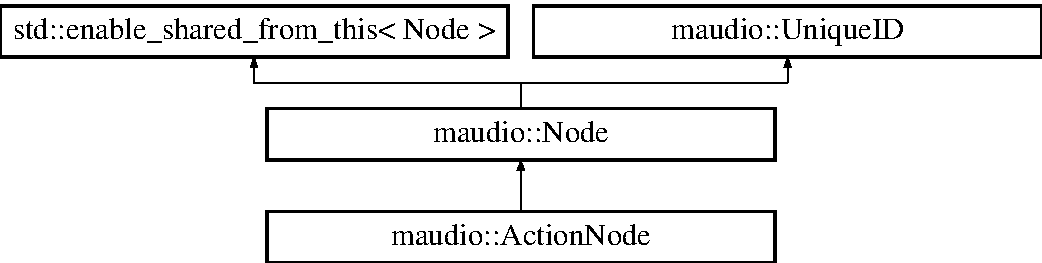
\includegraphics[height=3.000000cm]{classmaudio_1_1ActionNode}
\end{center}
\end{figure}
\subsection*{Classes}
\begin{DoxyCompactItemize}
\item 
class \hyperlink{classmaudio_1_1ActionNode_1_1Socket}{Socket}
\end{DoxyCompactItemize}
\subsection*{Public Member Functions}
\begin{DoxyCompactItemize}
\item 
\hyperlink{classmaudio_1_1ActionNode_a14305cfd931a5fbec4b194153a198f62}{Action\-Node} (\hyperlink{classmaudio_1_1IAction}{I\-Action} $\ast$action)
\item 
\hyperlink{classmaudio_1_1ActionNode_a7d47bb0a6d57b72f5fbe7b59bf1535c0}{Action\-Node} (std\-::unique\-\_\-ptr$<$ \hyperlink{classmaudio_1_1IAction}{I\-Action} $>$ action)
\item 
virtual \hyperlink{classmaudio_1_1ActionNode_a2fa5aaa6854ce58dfc02a04984473d5e}{$\sim$\-Action\-Node} ()
\item 
virtual \hyperlink{classmaudio_1_1IAudioBuffer}{I\-Audio\-Buffer} $\ast$ \hyperlink{classmaudio_1_1ActionNode_a7dad30c2c187519dfb8508a088a2d842}{get} (unsigned long pos, unsigned int length) noexcept
\item 
virtual \hyperlink{classmaudio_1_1IAudioInfo}{I\-Audio\-Info} $\ast$ \hyperlink{classmaudio_1_1ActionNode_a10c712ce5741eeeeb46fc8cadf9687b5}{get\-Info} () noexcept
\item 
virtual void \hyperlink{classmaudio_1_1ActionNode_ad89fda4bd963d3176ad61dfd414596a5}{delete\-Buffer} (\hyperlink{classmaudio_1_1IAudioBuffer}{I\-Audio\-Buffer} $\ast$data) noexcept
\item 
virtual void \hyperlink{classmaudio_1_1ActionNode_a2cedf925663e0c898fae99e826586e9a}{delete\-Info} (\hyperlink{classmaudio_1_1IAudioInfo}{I\-Audio\-Info} $\ast$data) noexcept
\item 
virtual void \hyperlink{classmaudio_1_1ActionNode_ac10ce0b12b802fb444c91999337ac3dc}{delete\-Sample} (\hyperlink{classmaudio_1_1ISample}{I\-Sample} $\ast$data) noexcept
\item 
virtual int \hyperlink{classmaudio_1_1ActionNode_a6e6e10558f7cc555f1dcbe2de6b5cdb2}{Max\-Inputs} () const 
\item 
virtual bool \hyperlink{classmaudio_1_1ActionNode_a7f43a61f1da08dd12688d5480677b8c1}{Has\-Outputs} () const 
\item 
virtual void \hyperlink{classmaudio_1_1ActionNode_aba178721f832128b48adc02550545ce1}{read\-Config} (const \hyperlink{classmaudio_1_1Config}{Config} \&conf)
\item 
virtual \hyperlink{classmaudio_1_1IPropertyManager}{I\-Property\-Manager} $\ast$ \hyperlink{classmaudio_1_1ActionNode_a8f9a10275ff3bf112c7f14e896d14c06}{get\-Properties} ()
\item 
virtual \hyperlink{classmaudio_1_1IControl}{I\-Control} $\ast$ \hyperlink{classmaudio_1_1ActionNode_aa4647a1e40a0ce5f3b19098ed347b5da}{get\-Control} ()
\item 
virtual \hyperlink{classmaudio_1_1IKeyValueStore}{I\-Key\-Value\-Store} $\ast$ \hyperlink{classmaudio_1_1ActionNode_a7aa30b6bf8a68cb222472f4e20d05b13}{serialize} () const 
\item 
virtual void \hyperlink{classmaudio_1_1ActionNode_a7e416ec107ebbcb1ed6c771cf35acab5}{deserialize} (const \hyperlink{classmaudio_1_1IKeyValueStore}{I\-Key\-Value\-Store} $\ast$data)
\end{DoxyCompactItemize}
\subsection*{Protected Member Functions}
\begin{DoxyCompactItemize}
\item 
virtual void \hyperlink{classmaudio_1_1ActionNode_ad2a0d41f2370fa8a32fc4e6ce2bb9eef}{on\-Add} (unsigned int slot)
\item 
virtual void \hyperlink{classmaudio_1_1ActionNode_aaa27a57824ba5e990d935ef117b6ef69}{on\-Remove} (unsigned int slot)
\end{DoxyCompactItemize}
\subsection*{Protected Attributes}
\begin{DoxyCompactItemize}
\item 
std\-::unique\-\_\-ptr$<$ \hyperlink{classmaudio_1_1IAction}{I\-Action} $>$ \hyperlink{classmaudio_1_1ActionNode_adac01f86f3fe16240528288f52729bc6}{m\-Action}
\end{DoxyCompactItemize}


\subsection{Constructor \& Destructor Documentation}
\hypertarget{classmaudio_1_1ActionNode_a14305cfd931a5fbec4b194153a198f62}{\index{maudio\-::\-Action\-Node@{maudio\-::\-Action\-Node}!Action\-Node@{Action\-Node}}
\index{Action\-Node@{Action\-Node}!maudio::ActionNode@{maudio\-::\-Action\-Node}}
\subsubsection[{Action\-Node}]{\setlength{\rightskip}{0pt plus 5cm}maudio\-::\-Action\-Node\-::\-Action\-Node (
\begin{DoxyParamCaption}
\item[{{\bf I\-Action} $\ast$}]{action}
\end{DoxyParamCaption}
)}}\label{classmaudio_1_1ActionNode_a14305cfd931a5fbec4b194153a198f62}
\hypertarget{classmaudio_1_1ActionNode_a7d47bb0a6d57b72f5fbe7b59bf1535c0}{\index{maudio\-::\-Action\-Node@{maudio\-::\-Action\-Node}!Action\-Node@{Action\-Node}}
\index{Action\-Node@{Action\-Node}!maudio::ActionNode@{maudio\-::\-Action\-Node}}
\subsubsection[{Action\-Node}]{\setlength{\rightskip}{0pt plus 5cm}maudio\-::\-Action\-Node\-::\-Action\-Node (
\begin{DoxyParamCaption}
\item[{std\-::unique\-\_\-ptr$<$ {\bf I\-Action} $>$}]{action}
\end{DoxyParamCaption}
)}}\label{classmaudio_1_1ActionNode_a7d47bb0a6d57b72f5fbe7b59bf1535c0}
\hypertarget{classmaudio_1_1ActionNode_a2fa5aaa6854ce58dfc02a04984473d5e}{\index{maudio\-::\-Action\-Node@{maudio\-::\-Action\-Node}!$\sim$\-Action\-Node@{$\sim$\-Action\-Node}}
\index{$\sim$\-Action\-Node@{$\sim$\-Action\-Node}!maudio::ActionNode@{maudio\-::\-Action\-Node}}
\subsubsection[{$\sim$\-Action\-Node}]{\setlength{\rightskip}{0pt plus 5cm}maudio\-::\-Action\-Node\-::$\sim$\-Action\-Node (
\begin{DoxyParamCaption}
{}
\end{DoxyParamCaption}
)\hspace{0.3cm}{\ttfamily [virtual]}}}\label{classmaudio_1_1ActionNode_a2fa5aaa6854ce58dfc02a04984473d5e}


\subsection{Member Function Documentation}
\hypertarget{classmaudio_1_1ActionNode_ad89fda4bd963d3176ad61dfd414596a5}{\index{maudio\-::\-Action\-Node@{maudio\-::\-Action\-Node}!delete\-Buffer@{delete\-Buffer}}
\index{delete\-Buffer@{delete\-Buffer}!maudio::ActionNode@{maudio\-::\-Action\-Node}}
\subsubsection[{delete\-Buffer}]{\setlength{\rightskip}{0pt plus 5cm}void maudio\-::\-Action\-Node\-::delete\-Buffer (
\begin{DoxyParamCaption}
\item[{{\bf I\-Audio\-Buffer} $\ast$}]{data}
\end{DoxyParamCaption}
)\hspace{0.3cm}{\ttfamily [virtual]}, {\ttfamily [noexcept]}}}\label{classmaudio_1_1ActionNode_ad89fda4bd963d3176ad61dfd414596a5}


Implements \hyperlink{classmaudio_1_1Node_a11f8c628cc1d1994ad45e9ea81d5e27c}{maudio\-::\-Node}.

\hypertarget{classmaudio_1_1ActionNode_a2cedf925663e0c898fae99e826586e9a}{\index{maudio\-::\-Action\-Node@{maudio\-::\-Action\-Node}!delete\-Info@{delete\-Info}}
\index{delete\-Info@{delete\-Info}!maudio::ActionNode@{maudio\-::\-Action\-Node}}
\subsubsection[{delete\-Info}]{\setlength{\rightskip}{0pt plus 5cm}void maudio\-::\-Action\-Node\-::delete\-Info (
\begin{DoxyParamCaption}
\item[{{\bf I\-Audio\-Info} $\ast$}]{data}
\end{DoxyParamCaption}
)\hspace{0.3cm}{\ttfamily [virtual]}, {\ttfamily [noexcept]}}}\label{classmaudio_1_1ActionNode_a2cedf925663e0c898fae99e826586e9a}


Implements \hyperlink{classmaudio_1_1Node_af9a851c3aa51799a416f4a42acb15617}{maudio\-::\-Node}.

\hypertarget{classmaudio_1_1ActionNode_ac10ce0b12b802fb444c91999337ac3dc}{\index{maudio\-::\-Action\-Node@{maudio\-::\-Action\-Node}!delete\-Sample@{delete\-Sample}}
\index{delete\-Sample@{delete\-Sample}!maudio::ActionNode@{maudio\-::\-Action\-Node}}
\subsubsection[{delete\-Sample}]{\setlength{\rightskip}{0pt plus 5cm}void maudio\-::\-Action\-Node\-::delete\-Sample (
\begin{DoxyParamCaption}
\item[{{\bf I\-Sample} $\ast$}]{data}
\end{DoxyParamCaption}
)\hspace{0.3cm}{\ttfamily [virtual]}, {\ttfamily [noexcept]}}}\label{classmaudio_1_1ActionNode_ac10ce0b12b802fb444c91999337ac3dc}


Implements \hyperlink{classmaudio_1_1Node_a4a6a5d0dc79d3bee44d3284517bdfe2b}{maudio\-::\-Node}.

\hypertarget{classmaudio_1_1ActionNode_a7e416ec107ebbcb1ed6c771cf35acab5}{\index{maudio\-::\-Action\-Node@{maudio\-::\-Action\-Node}!deserialize@{deserialize}}
\index{deserialize@{deserialize}!maudio::ActionNode@{maudio\-::\-Action\-Node}}
\subsubsection[{deserialize}]{\setlength{\rightskip}{0pt plus 5cm}void maudio\-::\-Action\-Node\-::deserialize (
\begin{DoxyParamCaption}
\item[{const {\bf I\-Key\-Value\-Store} $\ast$}]{data}
\end{DoxyParamCaption}
)\hspace{0.3cm}{\ttfamily [virtual]}}}\label{classmaudio_1_1ActionNode_a7e416ec107ebbcb1ed6c771cf35acab5}


Implements \hyperlink{classmaudio_1_1Node_af6be2a9f71d265bdbd5a230a58c8138c}{maudio\-::\-Node}.

\hypertarget{classmaudio_1_1ActionNode_a7dad30c2c187519dfb8508a088a2d842}{\index{maudio\-::\-Action\-Node@{maudio\-::\-Action\-Node}!get@{get}}
\index{get@{get}!maudio::ActionNode@{maudio\-::\-Action\-Node}}
\subsubsection[{get}]{\setlength{\rightskip}{0pt plus 5cm}{\bf I\-Audio\-Buffer} $\ast$ maudio\-::\-Action\-Node\-::get (
\begin{DoxyParamCaption}
\item[{unsigned long}]{pos, }
\item[{unsigned int}]{length}
\end{DoxyParamCaption}
)\hspace{0.3cm}{\ttfamily [virtual]}, {\ttfamily [noexcept]}}}\label{classmaudio_1_1ActionNode_a7dad30c2c187519dfb8508a088a2d842}


Implements \hyperlink{classmaudio_1_1Node_a19514a2d372ace1179e2b910b13ee26c}{maudio\-::\-Node}.

\hypertarget{classmaudio_1_1ActionNode_aa4647a1e40a0ce5f3b19098ed347b5da}{\index{maudio\-::\-Action\-Node@{maudio\-::\-Action\-Node}!get\-Control@{get\-Control}}
\index{get\-Control@{get\-Control}!maudio::ActionNode@{maudio\-::\-Action\-Node}}
\subsubsection[{get\-Control}]{\setlength{\rightskip}{0pt plus 5cm}{\bf I\-Control} $\ast$ maudio\-::\-Action\-Node\-::get\-Control (
\begin{DoxyParamCaption}
{}
\end{DoxyParamCaption}
)\hspace{0.3cm}{\ttfamily [virtual]}}}\label{classmaudio_1_1ActionNode_aa4647a1e40a0ce5f3b19098ed347b5da}


Implements \hyperlink{classmaudio_1_1Node_a4cf6cb717e8811c64bc018bae9248b9f}{maudio\-::\-Node}.

\hypertarget{classmaudio_1_1ActionNode_a10c712ce5741eeeeb46fc8cadf9687b5}{\index{maudio\-::\-Action\-Node@{maudio\-::\-Action\-Node}!get\-Info@{get\-Info}}
\index{get\-Info@{get\-Info}!maudio::ActionNode@{maudio\-::\-Action\-Node}}
\subsubsection[{get\-Info}]{\setlength{\rightskip}{0pt plus 5cm}{\bf I\-Audio\-Info} $\ast$ maudio\-::\-Action\-Node\-::get\-Info (
\begin{DoxyParamCaption}
{}
\end{DoxyParamCaption}
)\hspace{0.3cm}{\ttfamily [virtual]}, {\ttfamily [noexcept]}}}\label{classmaudio_1_1ActionNode_a10c712ce5741eeeeb46fc8cadf9687b5}


Implements \hyperlink{classmaudio_1_1Node_a7e8a3c69d7d49328dba7f0ab004a6bd4}{maudio\-::\-Node}.

\hypertarget{classmaudio_1_1ActionNode_a8f9a10275ff3bf112c7f14e896d14c06}{\index{maudio\-::\-Action\-Node@{maudio\-::\-Action\-Node}!get\-Properties@{get\-Properties}}
\index{get\-Properties@{get\-Properties}!maudio::ActionNode@{maudio\-::\-Action\-Node}}
\subsubsection[{get\-Properties}]{\setlength{\rightskip}{0pt plus 5cm}{\bf I\-Property\-Manager} $\ast$ maudio\-::\-Action\-Node\-::get\-Properties (
\begin{DoxyParamCaption}
{}
\end{DoxyParamCaption}
)\hspace{0.3cm}{\ttfamily [virtual]}}}\label{classmaudio_1_1ActionNode_a8f9a10275ff3bf112c7f14e896d14c06}


Implements \hyperlink{classmaudio_1_1Node_ac9960215fa9c0201f1fc31f4f206036c}{maudio\-::\-Node}.

\hypertarget{classmaudio_1_1ActionNode_a7f43a61f1da08dd12688d5480677b8c1}{\index{maudio\-::\-Action\-Node@{maudio\-::\-Action\-Node}!Has\-Outputs@{Has\-Outputs}}
\index{Has\-Outputs@{Has\-Outputs}!maudio::ActionNode@{maudio\-::\-Action\-Node}}
\subsubsection[{Has\-Outputs}]{\setlength{\rightskip}{0pt plus 5cm}bool maudio\-::\-Action\-Node\-::\-Has\-Outputs (
\begin{DoxyParamCaption}
{}
\end{DoxyParamCaption}
) const\hspace{0.3cm}{\ttfamily [virtual]}}}\label{classmaudio_1_1ActionNode_a7f43a61f1da08dd12688d5480677b8c1}


Implements \hyperlink{classmaudio_1_1Node_adefc8b35c3242b11730071d72dd8cf83}{maudio\-::\-Node}.

\hypertarget{classmaudio_1_1ActionNode_a6e6e10558f7cc555f1dcbe2de6b5cdb2}{\index{maudio\-::\-Action\-Node@{maudio\-::\-Action\-Node}!Max\-Inputs@{Max\-Inputs}}
\index{Max\-Inputs@{Max\-Inputs}!maudio::ActionNode@{maudio\-::\-Action\-Node}}
\subsubsection[{Max\-Inputs}]{\setlength{\rightskip}{0pt plus 5cm}int maudio\-::\-Action\-Node\-::\-Max\-Inputs (
\begin{DoxyParamCaption}
{}
\end{DoxyParamCaption}
) const\hspace{0.3cm}{\ttfamily [virtual]}}}\label{classmaudio_1_1ActionNode_a6e6e10558f7cc555f1dcbe2de6b5cdb2}


Implements \hyperlink{classmaudio_1_1Node_a2d3df13430b6ee1ba1a08a2bfc04d092}{maudio\-::\-Node}.

\hypertarget{classmaudio_1_1ActionNode_ad2a0d41f2370fa8a32fc4e6ce2bb9eef}{\index{maudio\-::\-Action\-Node@{maudio\-::\-Action\-Node}!on\-Add@{on\-Add}}
\index{on\-Add@{on\-Add}!maudio::ActionNode@{maudio\-::\-Action\-Node}}
\subsubsection[{on\-Add}]{\setlength{\rightskip}{0pt plus 5cm}void maudio\-::\-Action\-Node\-::on\-Add (
\begin{DoxyParamCaption}
\item[{unsigned int}]{slot}
\end{DoxyParamCaption}
)\hspace{0.3cm}{\ttfamily [protected]}, {\ttfamily [virtual]}}}\label{classmaudio_1_1ActionNode_ad2a0d41f2370fa8a32fc4e6ce2bb9eef}


Implements \hyperlink{classmaudio_1_1Node_aef1bcd3c5642c86495259b638ab54290}{maudio\-::\-Node}.

\hypertarget{classmaudio_1_1ActionNode_aaa27a57824ba5e990d935ef117b6ef69}{\index{maudio\-::\-Action\-Node@{maudio\-::\-Action\-Node}!on\-Remove@{on\-Remove}}
\index{on\-Remove@{on\-Remove}!maudio::ActionNode@{maudio\-::\-Action\-Node}}
\subsubsection[{on\-Remove}]{\setlength{\rightskip}{0pt plus 5cm}void maudio\-::\-Action\-Node\-::on\-Remove (
\begin{DoxyParamCaption}
\item[{unsigned int}]{slot}
\end{DoxyParamCaption}
)\hspace{0.3cm}{\ttfamily [protected]}, {\ttfamily [virtual]}}}\label{classmaudio_1_1ActionNode_aaa27a57824ba5e990d935ef117b6ef69}


Implements \hyperlink{classmaudio_1_1Node_a058346c2dddf4e1cb061fadbd433446e}{maudio\-::\-Node}.

\hypertarget{classmaudio_1_1ActionNode_aba178721f832128b48adc02550545ce1}{\index{maudio\-::\-Action\-Node@{maudio\-::\-Action\-Node}!read\-Config@{read\-Config}}
\index{read\-Config@{read\-Config}!maudio::ActionNode@{maudio\-::\-Action\-Node}}
\subsubsection[{read\-Config}]{\setlength{\rightskip}{0pt plus 5cm}void maudio\-::\-Action\-Node\-::read\-Config (
\begin{DoxyParamCaption}
\item[{const {\bf Config} \&}]{conf}
\end{DoxyParamCaption}
)\hspace{0.3cm}{\ttfamily [virtual]}}}\label{classmaudio_1_1ActionNode_aba178721f832128b48adc02550545ce1}


Implements \hyperlink{classmaudio_1_1Node_aab5537a1cda3ec0db8c7a91545066197}{maudio\-::\-Node}.

\hypertarget{classmaudio_1_1ActionNode_a7aa30b6bf8a68cb222472f4e20d05b13}{\index{maudio\-::\-Action\-Node@{maudio\-::\-Action\-Node}!serialize@{serialize}}
\index{serialize@{serialize}!maudio::ActionNode@{maudio\-::\-Action\-Node}}
\subsubsection[{serialize}]{\setlength{\rightskip}{0pt plus 5cm}{\bf I\-Key\-Value\-Store} $\ast$ maudio\-::\-Action\-Node\-::serialize (
\begin{DoxyParamCaption}
{}
\end{DoxyParamCaption}
) const\hspace{0.3cm}{\ttfamily [virtual]}}}\label{classmaudio_1_1ActionNode_a7aa30b6bf8a68cb222472f4e20d05b13}


Implements \hyperlink{classmaudio_1_1Node_a264737e69763b0aa28277c52a772a14f}{maudio\-::\-Node}.



\subsection{Member Data Documentation}
\hypertarget{classmaudio_1_1ActionNode_adac01f86f3fe16240528288f52729bc6}{\index{maudio\-::\-Action\-Node@{maudio\-::\-Action\-Node}!m\-Action@{m\-Action}}
\index{m\-Action@{m\-Action}!maudio::ActionNode@{maudio\-::\-Action\-Node}}
\subsubsection[{m\-Action}]{\setlength{\rightskip}{0pt plus 5cm}std\-::unique\-\_\-ptr$<${\bf I\-Action}$>$ maudio\-::\-Action\-Node\-::m\-Action\hspace{0.3cm}{\ttfamily [protected]}}}\label{classmaudio_1_1ActionNode_adac01f86f3fe16240528288f52729bc6}


The documentation for this class was generated from the following files\-:\begin{DoxyCompactItemize}
\item 
/home/mars/\-Projekte/maudio/src/plugins/include/core/node/\hyperlink{ActionNode_8hpp}{Action\-Node.\-hpp}\item 
/home/mars/\-Projekte/maudio/src/core/node/\hyperlink{core_2node_2ActionNode_8cpp}{Action\-Node.\-cpp}\end{DoxyCompactItemize}

\hypertarget{classmaudio_1_1AudioBuffer}{\section{maudio\-:\-:Audio\-Buffer Class Reference}
\label{classmaudio_1_1AudioBuffer}\index{maudio\-::\-Audio\-Buffer@{maudio\-::\-Audio\-Buffer}}
}


holds an audio stream in a vector of floats  




{\ttfamily \#include $<$Audio\-Buffer.\-hpp$>$}

Inheritance diagram for maudio\-:\-:Audio\-Buffer\-:\begin{figure}[H]
\begin{center}
\leavevmode
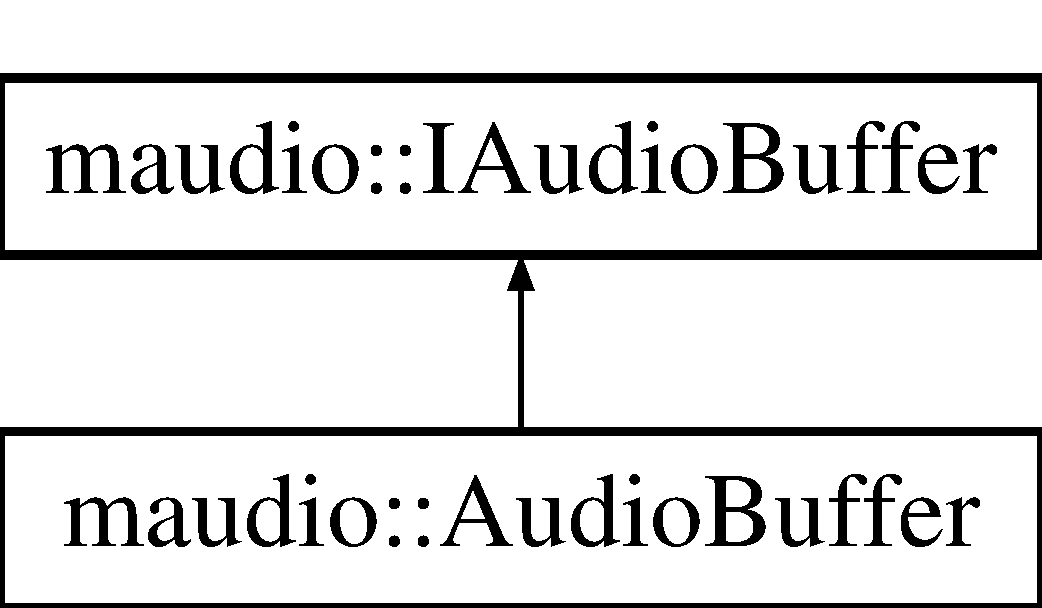
\includegraphics[height=2.000000cm]{classmaudio_1_1AudioBuffer}
\end{center}
\end{figure}
\subsection*{Public Member Functions}
\begin{DoxyCompactItemize}
\item 
\hyperlink{classmaudio_1_1AudioBuffer_aaf9868a32b5d236f05c18eab92dc8fbc}{Audio\-Buffer} (\hyperlink{classmaudio_1_1IAudioInfo}{I\-Audio\-Info} \&info)
\item 
\hyperlink{classmaudio_1_1AudioBuffer_aacc7c601e16cb298852e4cd8bf0b9877}{Audio\-Buffer} (unsigned int channels=1, unsigned long samples=0, unsigned long offset=0, unsigned int samplerate=44100)
\item 
\hyperlink{classmaudio_1_1AudioBuffer_a114fe8fbb88ebbd2bd10d2db87bfb72b}{Audio\-Buffer} (const \hyperlink{classmaudio_1_1AudioBuffer}{Audio\-Buffer} \&data)
\item 
virtual \hyperlink{classmaudio_1_1AudioBuffer_af8297698130918e9edcdfefaccdbd19c}{$\sim$\-Audio\-Buffer} ()
\item 
virtual \hyperlink{classmaudio_1_1ISample}{I\-Sample} $\ast$ \hyperlink{classmaudio_1_1AudioBuffer_a6548ddb981ec41fa92d821a15aa06080}{operator\mbox{[}$\,$\mbox{]}} (unsigned long pos) const 
\item 
virtual void \hyperlink{classmaudio_1_1AudioBuffer_afdd22331a8ac4e0643f2e0732be5b223}{operator=} (const \hyperlink{classmaudio_1_1IAudioBuffer}{I\-Audio\-Buffer} \&data)
\item 
virtual \hyperlink{classmaudio_1_1ISample}{I\-Sample} $\ast$ \hyperlink{classmaudio_1_1AudioBuffer_a93eeb4f2f16bf113e8bc77592d7c4664}{get} (unsigned long pos) const 
\item 
virtual void \hyperlink{classmaudio_1_1AudioBuffer_a3f19c9611c89947bbf27af7f788b8347}{set} (const \hyperlink{classmaudio_1_1ISample}{I\-Sample} \&data, unsigned long pos)
\item 
virtual void \hyperlink{classmaudio_1_1AudioBuffer_aeed134c3a1b7f5446594fa23c8857e8c}{resize} (unsigned long samples)
\item 
virtual const \hyperlink{classmaudio_1_1IAudioInfo}{I\-Audio\-Info} $\ast$ \hyperlink{classmaudio_1_1AudioBuffer_aa5e0294c0de7b4bbcaed0afa9ae22728}{get\-Info} () const 
\item 
virtual const float $\ast$ \hyperlink{classmaudio_1_1AudioBuffer_a6ac54537437e8a3fc4236b9375dc0126}{get\-Raw} () const 
\end{DoxyCompactItemize}


\subsection{Detailed Description}
holds an audio stream in a vector of floats 

\subsection{Constructor \& Destructor Documentation}
\hypertarget{classmaudio_1_1AudioBuffer_aaf9868a32b5d236f05c18eab92dc8fbc}{\index{maudio\-::\-Audio\-Buffer@{maudio\-::\-Audio\-Buffer}!Audio\-Buffer@{Audio\-Buffer}}
\index{Audio\-Buffer@{Audio\-Buffer}!maudio::AudioBuffer@{maudio\-::\-Audio\-Buffer}}
\subsubsection[{Audio\-Buffer}]{\setlength{\rightskip}{0pt plus 5cm}maudio\-::\-Audio\-Buffer\-::\-Audio\-Buffer (
\begin{DoxyParamCaption}
\item[{{\bf I\-Audio\-Info} \&}]{info}
\end{DoxyParamCaption}
)}}\label{classmaudio_1_1AudioBuffer_aaf9868a32b5d236f05c18eab92dc8fbc}
\hypertarget{classmaudio_1_1AudioBuffer_aacc7c601e16cb298852e4cd8bf0b9877}{\index{maudio\-::\-Audio\-Buffer@{maudio\-::\-Audio\-Buffer}!Audio\-Buffer@{Audio\-Buffer}}
\index{Audio\-Buffer@{Audio\-Buffer}!maudio::AudioBuffer@{maudio\-::\-Audio\-Buffer}}
\subsubsection[{Audio\-Buffer}]{\setlength{\rightskip}{0pt plus 5cm}maudio\-::\-Audio\-Buffer\-::\-Audio\-Buffer (
\begin{DoxyParamCaption}
\item[{unsigned int}]{channels = {\ttfamily 1}, }
\item[{unsigned long}]{samples = {\ttfamily 0}, }
\item[{unsigned long}]{offset = {\ttfamily 0}, }
\item[{unsigned int}]{samplerate = {\ttfamily 44100}}
\end{DoxyParamCaption}
)}}\label{classmaudio_1_1AudioBuffer_aacc7c601e16cb298852e4cd8bf0b9877}
\hypertarget{classmaudio_1_1AudioBuffer_a114fe8fbb88ebbd2bd10d2db87bfb72b}{\index{maudio\-::\-Audio\-Buffer@{maudio\-::\-Audio\-Buffer}!Audio\-Buffer@{Audio\-Buffer}}
\index{Audio\-Buffer@{Audio\-Buffer}!maudio::AudioBuffer@{maudio\-::\-Audio\-Buffer}}
\subsubsection[{Audio\-Buffer}]{\setlength{\rightskip}{0pt plus 5cm}maudio\-::\-Audio\-Buffer\-::\-Audio\-Buffer (
\begin{DoxyParamCaption}
\item[{const {\bf Audio\-Buffer} \&}]{data}
\end{DoxyParamCaption}
)}}\label{classmaudio_1_1AudioBuffer_a114fe8fbb88ebbd2bd10d2db87bfb72b}
\hypertarget{classmaudio_1_1AudioBuffer_af8297698130918e9edcdfefaccdbd19c}{\index{maudio\-::\-Audio\-Buffer@{maudio\-::\-Audio\-Buffer}!$\sim$\-Audio\-Buffer@{$\sim$\-Audio\-Buffer}}
\index{$\sim$\-Audio\-Buffer@{$\sim$\-Audio\-Buffer}!maudio::AudioBuffer@{maudio\-::\-Audio\-Buffer}}
\subsubsection[{$\sim$\-Audio\-Buffer}]{\setlength{\rightskip}{0pt plus 5cm}maudio\-::\-Audio\-Buffer\-::$\sim$\-Audio\-Buffer (
\begin{DoxyParamCaption}
{}
\end{DoxyParamCaption}
)\hspace{0.3cm}{\ttfamily [virtual]}}}\label{classmaudio_1_1AudioBuffer_af8297698130918e9edcdfefaccdbd19c}


\subsection{Member Function Documentation}
\hypertarget{classmaudio_1_1AudioBuffer_a93eeb4f2f16bf113e8bc77592d7c4664}{\index{maudio\-::\-Audio\-Buffer@{maudio\-::\-Audio\-Buffer}!get@{get}}
\index{get@{get}!maudio::AudioBuffer@{maudio\-::\-Audio\-Buffer}}
\subsubsection[{get}]{\setlength{\rightskip}{0pt plus 5cm}{\bf I\-Sample} $\ast$ maudio\-::\-Audio\-Buffer\-::get (
\begin{DoxyParamCaption}
\item[{unsigned long}]{pos}
\end{DoxyParamCaption}
) const\hspace{0.3cm}{\ttfamily [virtual]}}}\label{classmaudio_1_1AudioBuffer_a93eeb4f2f16bf113e8bc77592d7c4664}


Implements \hyperlink{classmaudio_1_1IAudioBuffer_aaea60a9702071ae0b12e9e616e72defb}{maudio\-::\-I\-Audio\-Buffer}.

\hypertarget{classmaudio_1_1AudioBuffer_aa5e0294c0de7b4bbcaed0afa9ae22728}{\index{maudio\-::\-Audio\-Buffer@{maudio\-::\-Audio\-Buffer}!get\-Info@{get\-Info}}
\index{get\-Info@{get\-Info}!maudio::AudioBuffer@{maudio\-::\-Audio\-Buffer}}
\subsubsection[{get\-Info}]{\setlength{\rightskip}{0pt plus 5cm}const {\bf I\-Audio\-Info} $\ast$ maudio\-::\-Audio\-Buffer\-::get\-Info (
\begin{DoxyParamCaption}
{}
\end{DoxyParamCaption}
) const\hspace{0.3cm}{\ttfamily [virtual]}}}\label{classmaudio_1_1AudioBuffer_aa5e0294c0de7b4bbcaed0afa9ae22728}


Implements \hyperlink{classmaudio_1_1IAudioBuffer_afd0eb3d169bade19e4508a4eaa2a07b4}{maudio\-::\-I\-Audio\-Buffer}.

\hypertarget{classmaudio_1_1AudioBuffer_a6ac54537437e8a3fc4236b9375dc0126}{\index{maudio\-::\-Audio\-Buffer@{maudio\-::\-Audio\-Buffer}!get\-Raw@{get\-Raw}}
\index{get\-Raw@{get\-Raw}!maudio::AudioBuffer@{maudio\-::\-Audio\-Buffer}}
\subsubsection[{get\-Raw}]{\setlength{\rightskip}{0pt plus 5cm}const float $\ast$ maudio\-::\-Audio\-Buffer\-::get\-Raw (
\begin{DoxyParamCaption}
{}
\end{DoxyParamCaption}
) const\hspace{0.3cm}{\ttfamily [virtual]}}}\label{classmaudio_1_1AudioBuffer_a6ac54537437e8a3fc4236b9375dc0126}


Implements \hyperlink{classmaudio_1_1IAudioBuffer_a60f486dc3d94b4c4f06df698e7848117}{maudio\-::\-I\-Audio\-Buffer}.

\hypertarget{classmaudio_1_1AudioBuffer_afdd22331a8ac4e0643f2e0732be5b223}{\index{maudio\-::\-Audio\-Buffer@{maudio\-::\-Audio\-Buffer}!operator=@{operator=}}
\index{operator=@{operator=}!maudio::AudioBuffer@{maudio\-::\-Audio\-Buffer}}
\subsubsection[{operator=}]{\setlength{\rightskip}{0pt plus 5cm}void maudio\-::\-Audio\-Buffer\-::operator= (
\begin{DoxyParamCaption}
\item[{const {\bf I\-Audio\-Buffer} \&}]{data}
\end{DoxyParamCaption}
)\hspace{0.3cm}{\ttfamily [virtual]}}}\label{classmaudio_1_1AudioBuffer_afdd22331a8ac4e0643f2e0732be5b223}
\hypertarget{classmaudio_1_1AudioBuffer_a6548ddb981ec41fa92d821a15aa06080}{\index{maudio\-::\-Audio\-Buffer@{maudio\-::\-Audio\-Buffer}!operator\mbox{[}$\,$\mbox{]}@{operator[]}}
\index{operator\mbox{[}$\,$\mbox{]}@{operator[]}!maudio::AudioBuffer@{maudio\-::\-Audio\-Buffer}}
\subsubsection[{operator[]}]{\setlength{\rightskip}{0pt plus 5cm}{\bf I\-Sample} $\ast$ maudio\-::\-Audio\-Buffer\-::operator\mbox{[}$\,$\mbox{]} (
\begin{DoxyParamCaption}
\item[{unsigned long}]{pos}
\end{DoxyParamCaption}
) const\hspace{0.3cm}{\ttfamily [virtual]}}}\label{classmaudio_1_1AudioBuffer_a6548ddb981ec41fa92d821a15aa06080}


Implements \hyperlink{classmaudio_1_1IAudioBuffer_a32a5742929553887a22e4d48be0e3763}{maudio\-::\-I\-Audio\-Buffer}.

\hypertarget{classmaudio_1_1AudioBuffer_aeed134c3a1b7f5446594fa23c8857e8c}{\index{maudio\-::\-Audio\-Buffer@{maudio\-::\-Audio\-Buffer}!resize@{resize}}
\index{resize@{resize}!maudio::AudioBuffer@{maudio\-::\-Audio\-Buffer}}
\subsubsection[{resize}]{\setlength{\rightskip}{0pt plus 5cm}void maudio\-::\-Audio\-Buffer\-::resize (
\begin{DoxyParamCaption}
\item[{unsigned long}]{samples}
\end{DoxyParamCaption}
)\hspace{0.3cm}{\ttfamily [virtual]}}}\label{classmaudio_1_1AudioBuffer_aeed134c3a1b7f5446594fa23c8857e8c}


Implements \hyperlink{classmaudio_1_1IAudioBuffer_a50d44964ef18c7dfd483fd0e68294d6b}{maudio\-::\-I\-Audio\-Buffer}.

\hypertarget{classmaudio_1_1AudioBuffer_a3f19c9611c89947bbf27af7f788b8347}{\index{maudio\-::\-Audio\-Buffer@{maudio\-::\-Audio\-Buffer}!set@{set}}
\index{set@{set}!maudio::AudioBuffer@{maudio\-::\-Audio\-Buffer}}
\subsubsection[{set}]{\setlength{\rightskip}{0pt plus 5cm}void maudio\-::\-Audio\-Buffer\-::set (
\begin{DoxyParamCaption}
\item[{const {\bf I\-Sample} \&}]{data, }
\item[{unsigned long}]{pos}
\end{DoxyParamCaption}
)\hspace{0.3cm}{\ttfamily [virtual]}}}\label{classmaudio_1_1AudioBuffer_a3f19c9611c89947bbf27af7f788b8347}


Implements \hyperlink{classmaudio_1_1IAudioBuffer_ab8f8728745907781bc31508d5816ef60}{maudio\-::\-I\-Audio\-Buffer}.



The documentation for this class was generated from the following files\-:\begin{DoxyCompactItemize}
\item 
/home/mars/\-Projekte/maudio/src/plugins/include/core/audiodata/\hyperlink{AudioBuffer_8hpp}{Audio\-Buffer.\-hpp}\item 
/home/mars/\-Projekte/maudio/src/core/audiodata/\hyperlink{core_2audiodata_2AudioBuffer_8cpp}{Audio\-Buffer.\-cpp}\end{DoxyCompactItemize}

\hypertarget{classmaudio_1_1AudioDevice}{\section{maudio\-:\-:Audio\-Device Class Reference}
\label{classmaudio_1_1AudioDevice}\index{maudio\-::\-Audio\-Device@{maudio\-::\-Audio\-Device}}
}


{\ttfamily \#include $<$Audio\-Device.\-hpp$>$}

\subsection*{Public Member Functions}
\begin{DoxyCompactItemize}
\item 
const int \hyperlink{classmaudio_1_1AudioDevice_a44b7c0cbe6d0139ad0934bbf30538418}{get\-I\-D} ()
\item 
const std\-::string \hyperlink{classmaudio_1_1AudioDevice_a19ac6648a7c059936945db5a9a35f67d}{get\-Name} ()
\item 
void \hyperlink{classmaudio_1_1AudioDevice_aa2367abb2cda0eebd2caf79dced76aa9}{play} (std\-::shared\-\_\-ptr$<$ \hyperlink{classmaudio_1_1AudioQueue}{Audio\-Queue} $>$ data)
\item 
void \hyperlink{classmaudio_1_1AudioDevice_a7633b000390e14423c9cb63888a7d1a3}{pause} ()
\item 
void \hyperlink{classmaudio_1_1AudioDevice_a6730776a14eee6866508ef81d0e45fb4}{unpause} ()
\item 
void \hyperlink{classmaudio_1_1AudioDevice_aeb1e37dfc0c375b8d6732ccb0b3de667}{stop} ()
\item 
int \hyperlink{classmaudio_1_1AudioDevice_af9f763b7fb50350dd31b750fc2ed8f42}{get\-Status} ()
\end{DoxyCompactItemize}
\subsection*{Static Public Member Functions}
\begin{DoxyCompactItemize}
\item 
static \hyperlink{classmaudio_1_1AudioDevice}{Audio\-Device} $\ast$ \hyperlink{classmaudio_1_1AudioDevice_ae2586aef95693bd4585d5394675871b7}{open} ()
\item 
static \hyperlink{classmaudio_1_1AudioDevice}{Audio\-Device} $\ast$ \hyperlink{classmaudio_1_1AudioDevice_a33316f60046e8bb1140b0a1806390f8b}{open} (int device)
\item 
static \hyperlink{classmaudio_1_1AudioDevice}{Audio\-Device} $\ast$ \hyperlink{classmaudio_1_1AudioDevice_a13f3baa0b78421ce9e5524bbb91b7d90}{open} (std\-::string \&device)
\item 
static std\-::vector$<$ std\-::string $>$ \hyperlink{classmaudio_1_1AudioDevice_afcfef078937e7b58007eb1bf6882861a}{list\-Devices} ()
\end{DoxyCompactItemize}


\subsection{Member Function Documentation}
\hypertarget{classmaudio_1_1AudioDevice_a44b7c0cbe6d0139ad0934bbf30538418}{\index{maudio\-::\-Audio\-Device@{maudio\-::\-Audio\-Device}!get\-I\-D@{get\-I\-D}}
\index{get\-I\-D@{get\-I\-D}!maudio::AudioDevice@{maudio\-::\-Audio\-Device}}
\subsubsection[{get\-I\-D}]{\setlength{\rightskip}{0pt plus 5cm}const int maudio\-::\-Audio\-Device\-::get\-I\-D (
\begin{DoxyParamCaption}
{}
\end{DoxyParamCaption}
)}}\label{classmaudio_1_1AudioDevice_a44b7c0cbe6d0139ad0934bbf30538418}
\hypertarget{classmaudio_1_1AudioDevice_a19ac6648a7c059936945db5a9a35f67d}{\index{maudio\-::\-Audio\-Device@{maudio\-::\-Audio\-Device}!get\-Name@{get\-Name}}
\index{get\-Name@{get\-Name}!maudio::AudioDevice@{maudio\-::\-Audio\-Device}}
\subsubsection[{get\-Name}]{\setlength{\rightskip}{0pt plus 5cm}const std\-::string maudio\-::\-Audio\-Device\-::get\-Name (
\begin{DoxyParamCaption}
{}
\end{DoxyParamCaption}
)}}\label{classmaudio_1_1AudioDevice_a19ac6648a7c059936945db5a9a35f67d}
\hypertarget{classmaudio_1_1AudioDevice_af9f763b7fb50350dd31b750fc2ed8f42}{\index{maudio\-::\-Audio\-Device@{maudio\-::\-Audio\-Device}!get\-Status@{get\-Status}}
\index{get\-Status@{get\-Status}!maudio::AudioDevice@{maudio\-::\-Audio\-Device}}
\subsubsection[{get\-Status}]{\setlength{\rightskip}{0pt plus 5cm}int maudio\-::\-Audio\-Device\-::get\-Status (
\begin{DoxyParamCaption}
{}
\end{DoxyParamCaption}
)}}\label{classmaudio_1_1AudioDevice_af9f763b7fb50350dd31b750fc2ed8f42}
\hypertarget{classmaudio_1_1AudioDevice_afcfef078937e7b58007eb1bf6882861a}{\index{maudio\-::\-Audio\-Device@{maudio\-::\-Audio\-Device}!list\-Devices@{list\-Devices}}
\index{list\-Devices@{list\-Devices}!maudio::AudioDevice@{maudio\-::\-Audio\-Device}}
\subsubsection[{list\-Devices}]{\setlength{\rightskip}{0pt plus 5cm}std\-::vector$<$ std\-::string $>$ maudio\-::\-Audio\-Device\-::list\-Devices (
\begin{DoxyParamCaption}
{}
\end{DoxyParamCaption}
)\hspace{0.3cm}{\ttfamily [static]}}}\label{classmaudio_1_1AudioDevice_afcfef078937e7b58007eb1bf6882861a}
\hypertarget{classmaudio_1_1AudioDevice_ae2586aef95693bd4585d5394675871b7}{\index{maudio\-::\-Audio\-Device@{maudio\-::\-Audio\-Device}!open@{open}}
\index{open@{open}!maudio::AudioDevice@{maudio\-::\-Audio\-Device}}
\subsubsection[{open}]{\setlength{\rightskip}{0pt plus 5cm}{\bf Audio\-Device} $\ast$ maudio\-::\-Audio\-Device\-::open (
\begin{DoxyParamCaption}
{}
\end{DoxyParamCaption}
)\hspace{0.3cm}{\ttfamily [static]}}}\label{classmaudio_1_1AudioDevice_ae2586aef95693bd4585d5394675871b7}
\hypertarget{classmaudio_1_1AudioDevice_a33316f60046e8bb1140b0a1806390f8b}{\index{maudio\-::\-Audio\-Device@{maudio\-::\-Audio\-Device}!open@{open}}
\index{open@{open}!maudio::AudioDevice@{maudio\-::\-Audio\-Device}}
\subsubsection[{open}]{\setlength{\rightskip}{0pt plus 5cm}{\bf Audio\-Device} $\ast$ maudio\-::\-Audio\-Device\-::open (
\begin{DoxyParamCaption}
\item[{int}]{device}
\end{DoxyParamCaption}
)\hspace{0.3cm}{\ttfamily [static]}}}\label{classmaudio_1_1AudioDevice_a33316f60046e8bb1140b0a1806390f8b}
\hypertarget{classmaudio_1_1AudioDevice_a13f3baa0b78421ce9e5524bbb91b7d90}{\index{maudio\-::\-Audio\-Device@{maudio\-::\-Audio\-Device}!open@{open}}
\index{open@{open}!maudio::AudioDevice@{maudio\-::\-Audio\-Device}}
\subsubsection[{open}]{\setlength{\rightskip}{0pt plus 5cm}{\bf Audio\-Device} $\ast$ maudio\-::\-Audio\-Device\-::open (
\begin{DoxyParamCaption}
\item[{std\-::string \&}]{device}
\end{DoxyParamCaption}
)\hspace{0.3cm}{\ttfamily [static]}}}\label{classmaudio_1_1AudioDevice_a13f3baa0b78421ce9e5524bbb91b7d90}
\hypertarget{classmaudio_1_1AudioDevice_a7633b000390e14423c9cb63888a7d1a3}{\index{maudio\-::\-Audio\-Device@{maudio\-::\-Audio\-Device}!pause@{pause}}
\index{pause@{pause}!maudio::AudioDevice@{maudio\-::\-Audio\-Device}}
\subsubsection[{pause}]{\setlength{\rightskip}{0pt plus 5cm}void maudio\-::\-Audio\-Device\-::pause (
\begin{DoxyParamCaption}
{}
\end{DoxyParamCaption}
)}}\label{classmaudio_1_1AudioDevice_a7633b000390e14423c9cb63888a7d1a3}
\hypertarget{classmaudio_1_1AudioDevice_aa2367abb2cda0eebd2caf79dced76aa9}{\index{maudio\-::\-Audio\-Device@{maudio\-::\-Audio\-Device}!play@{play}}
\index{play@{play}!maudio::AudioDevice@{maudio\-::\-Audio\-Device}}
\subsubsection[{play}]{\setlength{\rightskip}{0pt plus 5cm}void maudio\-::\-Audio\-Device\-::play (
\begin{DoxyParamCaption}
\item[{std\-::shared\-\_\-ptr$<$ {\bf Audio\-Queue} $>$}]{data}
\end{DoxyParamCaption}
)}}\label{classmaudio_1_1AudioDevice_aa2367abb2cda0eebd2caf79dced76aa9}
\hypertarget{classmaudio_1_1AudioDevice_aeb1e37dfc0c375b8d6732ccb0b3de667}{\index{maudio\-::\-Audio\-Device@{maudio\-::\-Audio\-Device}!stop@{stop}}
\index{stop@{stop}!maudio::AudioDevice@{maudio\-::\-Audio\-Device}}
\subsubsection[{stop}]{\setlength{\rightskip}{0pt plus 5cm}void maudio\-::\-Audio\-Device\-::stop (
\begin{DoxyParamCaption}
{}
\end{DoxyParamCaption}
)}}\label{classmaudio_1_1AudioDevice_aeb1e37dfc0c375b8d6732ccb0b3de667}
\hypertarget{classmaudio_1_1AudioDevice_a6730776a14eee6866508ef81d0e45fb4}{\index{maudio\-::\-Audio\-Device@{maudio\-::\-Audio\-Device}!unpause@{unpause}}
\index{unpause@{unpause}!maudio::AudioDevice@{maudio\-::\-Audio\-Device}}
\subsubsection[{unpause}]{\setlength{\rightskip}{0pt plus 5cm}void maudio\-::\-Audio\-Device\-::unpause (
\begin{DoxyParamCaption}
{}
\end{DoxyParamCaption}
)}}\label{classmaudio_1_1AudioDevice_a6730776a14eee6866508ef81d0e45fb4}


The documentation for this class was generated from the following files\-:\begin{DoxyCompactItemize}
\item 
/home/mars/\-Projekte/maudio/src/extended/util/\hyperlink{AudioDevice_8hpp}{Audio\-Device.\-hpp}\item 
/home/mars/\-Projekte/maudio/src/extended/util/\hyperlink{AudioDevice_8cpp}{Audio\-Device.\-cpp}\end{DoxyCompactItemize}

\hypertarget{classmaudio_1_1AudioInfo}{\section{maudio\-:\-:Audio\-Info Class Reference}
\label{classmaudio_1_1AudioInfo}\index{maudio\-::\-Audio\-Info@{maudio\-::\-Audio\-Info}}
}


{\ttfamily \#include $<$Audio\-Info.\-hpp$>$}

Inheritance diagram for maudio\-:\-:Audio\-Info\-:\begin{figure}[H]
\begin{center}
\leavevmode
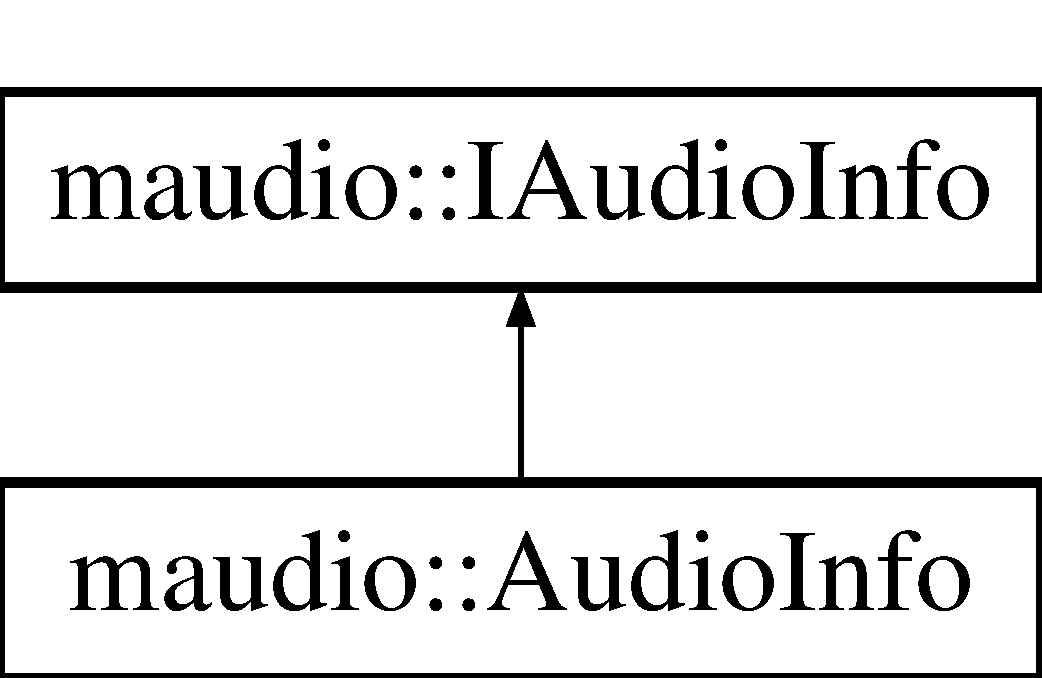
\includegraphics[height=2.000000cm]{classmaudio_1_1AudioInfo}
\end{center}
\end{figure}
\subsection*{Public Member Functions}
\begin{DoxyCompactItemize}
\item 
\hyperlink{classmaudio_1_1AudioInfo_ae955697a3221c6804495b68c3c8b9a1e}{Audio\-Info} ()
\item 
virtual \hyperlink{classmaudio_1_1AudioInfo_a154342e6963bcfe9f763e0db3c938205}{$\sim$\-Audio\-Info} ()
\item 
virtual unsigned long \hyperlink{classmaudio_1_1AudioInfo_aefb17a9c4301d9dcf6e5c04597892dbd}{get\-Samples} () const 
\item 
virtual unsigned long \hyperlink{classmaudio_1_1AudioInfo_ad89ed92138ad9e3e5b098bee69a9bd96}{get\-Offset} () const 
\item 
virtual unsigned int \hyperlink{classmaudio_1_1AudioInfo_a92e76f5173ea34dfdd0ca42ff0662a6f}{get\-Samplerate} () const 
\item 
virtual unsigned int \hyperlink{classmaudio_1_1AudioInfo_af4d1f9d433e4d29e218ec28bee4ed7db}{get\-Channels} () const 
\item 
virtual void \hyperlink{classmaudio_1_1AudioInfo_aa75d37ecf53cca3a0b7cecfb004da207}{set\-Samples} (unsigned long samples)
\item 
virtual void \hyperlink{classmaudio_1_1AudioInfo_aa1db33ccc763532a5d2858c00b65303a}{set\-Offset} (unsigned long offset)
\item 
virtual void \hyperlink{classmaudio_1_1AudioInfo_a5c466cc04ed7611522ad9ab626b101f5}{set\-Samplerate} (unsigned int samplerate)
\item 
virtual void \hyperlink{classmaudio_1_1AudioInfo_addb04eb7024304a625ef9304fa03dee9}{set\-Channels} (unsigned int channels)
\item 
virtual void \hyperlink{classmaudio_1_1AudioInfo_af407534e7d1ab48005dfb6e43127a0d0}{operator=} (const \hyperlink{classmaudio_1_1IAudioInfo}{I\-Audio\-Info} \&info)
\end{DoxyCompactItemize}


\subsection{Constructor \& Destructor Documentation}
\hypertarget{classmaudio_1_1AudioInfo_ae955697a3221c6804495b68c3c8b9a1e}{\index{maudio\-::\-Audio\-Info@{maudio\-::\-Audio\-Info}!Audio\-Info@{Audio\-Info}}
\index{Audio\-Info@{Audio\-Info}!maudio::AudioInfo@{maudio\-::\-Audio\-Info}}
\subsubsection[{Audio\-Info}]{\setlength{\rightskip}{0pt plus 5cm}maudio\-::\-Audio\-Info\-::\-Audio\-Info (
\begin{DoxyParamCaption}
{}
\end{DoxyParamCaption}
)\hspace{0.3cm}{\ttfamily [inline]}}}\label{classmaudio_1_1AudioInfo_ae955697a3221c6804495b68c3c8b9a1e}
\hypertarget{classmaudio_1_1AudioInfo_a154342e6963bcfe9f763e0db3c938205}{\index{maudio\-::\-Audio\-Info@{maudio\-::\-Audio\-Info}!$\sim$\-Audio\-Info@{$\sim$\-Audio\-Info}}
\index{$\sim$\-Audio\-Info@{$\sim$\-Audio\-Info}!maudio::AudioInfo@{maudio\-::\-Audio\-Info}}
\subsubsection[{$\sim$\-Audio\-Info}]{\setlength{\rightskip}{0pt plus 5cm}virtual maudio\-::\-Audio\-Info\-::$\sim$\-Audio\-Info (
\begin{DoxyParamCaption}
{}
\end{DoxyParamCaption}
)\hspace{0.3cm}{\ttfamily [inline]}, {\ttfamily [virtual]}}}\label{classmaudio_1_1AudioInfo_a154342e6963bcfe9f763e0db3c938205}


\subsection{Member Function Documentation}
\hypertarget{classmaudio_1_1AudioInfo_af4d1f9d433e4d29e218ec28bee4ed7db}{\index{maudio\-::\-Audio\-Info@{maudio\-::\-Audio\-Info}!get\-Channels@{get\-Channels}}
\index{get\-Channels@{get\-Channels}!maudio::AudioInfo@{maudio\-::\-Audio\-Info}}
\subsubsection[{get\-Channels}]{\setlength{\rightskip}{0pt plus 5cm}virtual unsigned int maudio\-::\-Audio\-Info\-::get\-Channels (
\begin{DoxyParamCaption}
{}
\end{DoxyParamCaption}
) const\hspace{0.3cm}{\ttfamily [inline]}, {\ttfamily [virtual]}}}\label{classmaudio_1_1AudioInfo_af4d1f9d433e4d29e218ec28bee4ed7db}


Implements \hyperlink{classmaudio_1_1IAudioInfo_a5b412da4d44d7939b4927ec932c74a83}{maudio\-::\-I\-Audio\-Info}.

\hypertarget{classmaudio_1_1AudioInfo_ad89ed92138ad9e3e5b098bee69a9bd96}{\index{maudio\-::\-Audio\-Info@{maudio\-::\-Audio\-Info}!get\-Offset@{get\-Offset}}
\index{get\-Offset@{get\-Offset}!maudio::AudioInfo@{maudio\-::\-Audio\-Info}}
\subsubsection[{get\-Offset}]{\setlength{\rightskip}{0pt plus 5cm}virtual unsigned long maudio\-::\-Audio\-Info\-::get\-Offset (
\begin{DoxyParamCaption}
{}
\end{DoxyParamCaption}
) const\hspace{0.3cm}{\ttfamily [inline]}, {\ttfamily [virtual]}}}\label{classmaudio_1_1AudioInfo_ad89ed92138ad9e3e5b098bee69a9bd96}


Implements \hyperlink{classmaudio_1_1IAudioInfo_ab85da546b049d23c400c8a869ea1e103}{maudio\-::\-I\-Audio\-Info}.

\hypertarget{classmaudio_1_1AudioInfo_a92e76f5173ea34dfdd0ca42ff0662a6f}{\index{maudio\-::\-Audio\-Info@{maudio\-::\-Audio\-Info}!get\-Samplerate@{get\-Samplerate}}
\index{get\-Samplerate@{get\-Samplerate}!maudio::AudioInfo@{maudio\-::\-Audio\-Info}}
\subsubsection[{get\-Samplerate}]{\setlength{\rightskip}{0pt plus 5cm}virtual unsigned int maudio\-::\-Audio\-Info\-::get\-Samplerate (
\begin{DoxyParamCaption}
{}
\end{DoxyParamCaption}
) const\hspace{0.3cm}{\ttfamily [inline]}, {\ttfamily [virtual]}}}\label{classmaudio_1_1AudioInfo_a92e76f5173ea34dfdd0ca42ff0662a6f}


Implements \hyperlink{classmaudio_1_1IAudioInfo_a557f464eb6a2feb2ce24dfae5a85d727}{maudio\-::\-I\-Audio\-Info}.

\hypertarget{classmaudio_1_1AudioInfo_aefb17a9c4301d9dcf6e5c04597892dbd}{\index{maudio\-::\-Audio\-Info@{maudio\-::\-Audio\-Info}!get\-Samples@{get\-Samples}}
\index{get\-Samples@{get\-Samples}!maudio::AudioInfo@{maudio\-::\-Audio\-Info}}
\subsubsection[{get\-Samples}]{\setlength{\rightskip}{0pt plus 5cm}virtual unsigned long maudio\-::\-Audio\-Info\-::get\-Samples (
\begin{DoxyParamCaption}
{}
\end{DoxyParamCaption}
) const\hspace{0.3cm}{\ttfamily [inline]}, {\ttfamily [virtual]}}}\label{classmaudio_1_1AudioInfo_aefb17a9c4301d9dcf6e5c04597892dbd}


Implements \hyperlink{classmaudio_1_1IAudioInfo_a88a698d7169f5c21118b83b8afcd1bf6}{maudio\-::\-I\-Audio\-Info}.

\hypertarget{classmaudio_1_1AudioInfo_af407534e7d1ab48005dfb6e43127a0d0}{\index{maudio\-::\-Audio\-Info@{maudio\-::\-Audio\-Info}!operator=@{operator=}}
\index{operator=@{operator=}!maudio::AudioInfo@{maudio\-::\-Audio\-Info}}
\subsubsection[{operator=}]{\setlength{\rightskip}{0pt plus 5cm}virtual void maudio\-::\-Audio\-Info\-::operator= (
\begin{DoxyParamCaption}
\item[{const {\bf I\-Audio\-Info} \&}]{info}
\end{DoxyParamCaption}
)\hspace{0.3cm}{\ttfamily [inline]}, {\ttfamily [virtual]}}}\label{classmaudio_1_1AudioInfo_af407534e7d1ab48005dfb6e43127a0d0}
\hypertarget{classmaudio_1_1AudioInfo_addb04eb7024304a625ef9304fa03dee9}{\index{maudio\-::\-Audio\-Info@{maudio\-::\-Audio\-Info}!set\-Channels@{set\-Channels}}
\index{set\-Channels@{set\-Channels}!maudio::AudioInfo@{maudio\-::\-Audio\-Info}}
\subsubsection[{set\-Channels}]{\setlength{\rightskip}{0pt plus 5cm}virtual void maudio\-::\-Audio\-Info\-::set\-Channels (
\begin{DoxyParamCaption}
\item[{unsigned int}]{channels}
\end{DoxyParamCaption}
)\hspace{0.3cm}{\ttfamily [inline]}, {\ttfamily [virtual]}}}\label{classmaudio_1_1AudioInfo_addb04eb7024304a625ef9304fa03dee9}


Implements \hyperlink{classmaudio_1_1IAudioInfo_aaae3741d16b6c0dc531084876940a0f4}{maudio\-::\-I\-Audio\-Info}.

\hypertarget{classmaudio_1_1AudioInfo_aa1db33ccc763532a5d2858c00b65303a}{\index{maudio\-::\-Audio\-Info@{maudio\-::\-Audio\-Info}!set\-Offset@{set\-Offset}}
\index{set\-Offset@{set\-Offset}!maudio::AudioInfo@{maudio\-::\-Audio\-Info}}
\subsubsection[{set\-Offset}]{\setlength{\rightskip}{0pt plus 5cm}virtual void maudio\-::\-Audio\-Info\-::set\-Offset (
\begin{DoxyParamCaption}
\item[{unsigned long}]{offset}
\end{DoxyParamCaption}
)\hspace{0.3cm}{\ttfamily [inline]}, {\ttfamily [virtual]}}}\label{classmaudio_1_1AudioInfo_aa1db33ccc763532a5d2858c00b65303a}


Implements \hyperlink{classmaudio_1_1IAudioInfo_a333fc60d8bf76b82bc0a65b8c6a77e4f}{maudio\-::\-I\-Audio\-Info}.

\hypertarget{classmaudio_1_1AudioInfo_a5c466cc04ed7611522ad9ab626b101f5}{\index{maudio\-::\-Audio\-Info@{maudio\-::\-Audio\-Info}!set\-Samplerate@{set\-Samplerate}}
\index{set\-Samplerate@{set\-Samplerate}!maudio::AudioInfo@{maudio\-::\-Audio\-Info}}
\subsubsection[{set\-Samplerate}]{\setlength{\rightskip}{0pt plus 5cm}virtual void maudio\-::\-Audio\-Info\-::set\-Samplerate (
\begin{DoxyParamCaption}
\item[{unsigned int}]{samplerate}
\end{DoxyParamCaption}
)\hspace{0.3cm}{\ttfamily [inline]}, {\ttfamily [virtual]}}}\label{classmaudio_1_1AudioInfo_a5c466cc04ed7611522ad9ab626b101f5}


Implements \hyperlink{classmaudio_1_1IAudioInfo_a2a54df3fc726ccb2b0994bc8e3d15c37}{maudio\-::\-I\-Audio\-Info}.

\hypertarget{classmaudio_1_1AudioInfo_aa75d37ecf53cca3a0b7cecfb004da207}{\index{maudio\-::\-Audio\-Info@{maudio\-::\-Audio\-Info}!set\-Samples@{set\-Samples}}
\index{set\-Samples@{set\-Samples}!maudio::AudioInfo@{maudio\-::\-Audio\-Info}}
\subsubsection[{set\-Samples}]{\setlength{\rightskip}{0pt plus 5cm}virtual void maudio\-::\-Audio\-Info\-::set\-Samples (
\begin{DoxyParamCaption}
\item[{unsigned long}]{samples}
\end{DoxyParamCaption}
)\hspace{0.3cm}{\ttfamily [inline]}, {\ttfamily [virtual]}}}\label{classmaudio_1_1AudioInfo_aa75d37ecf53cca3a0b7cecfb004da207}


Implements \hyperlink{classmaudio_1_1IAudioInfo_ab2b4c49c21fa711f457650cc377271bb}{maudio\-::\-I\-Audio\-Info}.



The documentation for this class was generated from the following file\-:\begin{DoxyCompactItemize}
\item 
/home/mars/\-Projekte/maudio/src/plugins/include/core/audiodata/\hyperlink{AudioInfo_8hpp}{Audio\-Info.\-hpp}\end{DoxyCompactItemize}

\hypertarget{classmaudio_1_1AudioQueue}{\section{maudio\-:\-:Audio\-Queue Class Reference}
\label{classmaudio_1_1AudioQueue}\index{maudio\-::\-Audio\-Queue@{maudio\-::\-Audio\-Queue}}
}


{\ttfamily \#include $<$Audio\-Queue.\-hpp$>$}

\subsection*{Public Member Functions}
\begin{DoxyCompactItemize}
\item 
\hyperlink{classmaudio_1_1AudioQueue_a3f4742df4c99cf2b6f912ad9add036de}{Audio\-Queue} (\hyperlink{classmaudio_1_1AudioInfo}{Audio\-Info} info)
\item 
void \hyperlink{classmaudio_1_1AudioQueue_a474f213d8948670ad4e89bcc4a01dee4}{push} (\hyperlink{classmaudio_1_1Sample}{Sample} data)
\item 
\hyperlink{classmaudio_1_1Sample}{Sample} \hyperlink{classmaudio_1_1AudioQueue_a7da087e1c3dfe44225fecf0d303a8037}{pop} ()
\item 
\hyperlink{classmaudio_1_1Sample}{Sample} \hyperlink{classmaudio_1_1AudioQueue_a641ec6f12f1ea9c1f2aa667e1205c781}{get} (unsigned long pos)
\item 
unsigned int \hyperlink{classmaudio_1_1AudioQueue_acb1a991997faa307caead887653a51c8}{get\-Channels} ()
\item 
unsigned int \hyperlink{classmaudio_1_1AudioQueue_abf78dafaa5176ace2bff357a8c5ffb52}{size} ()
\item 
\hyperlink{classmaudio_1_1AudioInfo}{Audio\-Info} \hyperlink{classmaudio_1_1AudioQueue_a904d256bed1fd4dd8057fc55bdf9e80c}{get\-Audio\-Info} ()
\item 
void \hyperlink{classmaudio_1_1AudioQueue_a618b63633c1ae578dc9ccc379dea4e41}{set\-Audio\-Info} (\hyperlink{classmaudio_1_1AudioInfo}{Audio\-Info} info)
\end{DoxyCompactItemize}


\subsection{Constructor \& Destructor Documentation}
\hypertarget{classmaudio_1_1AudioQueue_a3f4742df4c99cf2b6f912ad9add036de}{\index{maudio\-::\-Audio\-Queue@{maudio\-::\-Audio\-Queue}!Audio\-Queue@{Audio\-Queue}}
\index{Audio\-Queue@{Audio\-Queue}!maudio::AudioQueue@{maudio\-::\-Audio\-Queue}}
\subsubsection[{Audio\-Queue}]{\setlength{\rightskip}{0pt plus 5cm}maudio\-::\-Audio\-Queue\-::\-Audio\-Queue (
\begin{DoxyParamCaption}
\item[{{\bf Audio\-Info}}]{info}
\end{DoxyParamCaption}
)}}\label{classmaudio_1_1AudioQueue_a3f4742df4c99cf2b6f912ad9add036de}


\subsection{Member Function Documentation}
\hypertarget{classmaudio_1_1AudioQueue_a641ec6f12f1ea9c1f2aa667e1205c781}{\index{maudio\-::\-Audio\-Queue@{maudio\-::\-Audio\-Queue}!get@{get}}
\index{get@{get}!maudio::AudioQueue@{maudio\-::\-Audio\-Queue}}
\subsubsection[{get}]{\setlength{\rightskip}{0pt plus 5cm}{\bf Sample} maudio\-::\-Audio\-Queue\-::get (
\begin{DoxyParamCaption}
\item[{unsigned long}]{pos}
\end{DoxyParamCaption}
)}}\label{classmaudio_1_1AudioQueue_a641ec6f12f1ea9c1f2aa667e1205c781}
\hypertarget{classmaudio_1_1AudioQueue_a904d256bed1fd4dd8057fc55bdf9e80c}{\index{maudio\-::\-Audio\-Queue@{maudio\-::\-Audio\-Queue}!get\-Audio\-Info@{get\-Audio\-Info}}
\index{get\-Audio\-Info@{get\-Audio\-Info}!maudio::AudioQueue@{maudio\-::\-Audio\-Queue}}
\subsubsection[{get\-Audio\-Info}]{\setlength{\rightskip}{0pt plus 5cm}{\bf Audio\-Info} maudio\-::\-Audio\-Queue\-::get\-Audio\-Info (
\begin{DoxyParamCaption}
{}
\end{DoxyParamCaption}
)}}\label{classmaudio_1_1AudioQueue_a904d256bed1fd4dd8057fc55bdf9e80c}
\hypertarget{classmaudio_1_1AudioQueue_acb1a991997faa307caead887653a51c8}{\index{maudio\-::\-Audio\-Queue@{maudio\-::\-Audio\-Queue}!get\-Channels@{get\-Channels}}
\index{get\-Channels@{get\-Channels}!maudio::AudioQueue@{maudio\-::\-Audio\-Queue}}
\subsubsection[{get\-Channels}]{\setlength{\rightskip}{0pt plus 5cm}unsigned int maudio\-::\-Audio\-Queue\-::get\-Channels (
\begin{DoxyParamCaption}
{}
\end{DoxyParamCaption}
)}}\label{classmaudio_1_1AudioQueue_acb1a991997faa307caead887653a51c8}
\hypertarget{classmaudio_1_1AudioQueue_a7da087e1c3dfe44225fecf0d303a8037}{\index{maudio\-::\-Audio\-Queue@{maudio\-::\-Audio\-Queue}!pop@{pop}}
\index{pop@{pop}!maudio::AudioQueue@{maudio\-::\-Audio\-Queue}}
\subsubsection[{pop}]{\setlength{\rightskip}{0pt plus 5cm}{\bf Sample} maudio\-::\-Audio\-Queue\-::pop (
\begin{DoxyParamCaption}
{}
\end{DoxyParamCaption}
)}}\label{classmaudio_1_1AudioQueue_a7da087e1c3dfe44225fecf0d303a8037}
\hypertarget{classmaudio_1_1AudioQueue_a474f213d8948670ad4e89bcc4a01dee4}{\index{maudio\-::\-Audio\-Queue@{maudio\-::\-Audio\-Queue}!push@{push}}
\index{push@{push}!maudio::AudioQueue@{maudio\-::\-Audio\-Queue}}
\subsubsection[{push}]{\setlength{\rightskip}{0pt plus 5cm}void maudio\-::\-Audio\-Queue\-::push (
\begin{DoxyParamCaption}
\item[{{\bf Sample}}]{data}
\end{DoxyParamCaption}
)}}\label{classmaudio_1_1AudioQueue_a474f213d8948670ad4e89bcc4a01dee4}
\hypertarget{classmaudio_1_1AudioQueue_a618b63633c1ae578dc9ccc379dea4e41}{\index{maudio\-::\-Audio\-Queue@{maudio\-::\-Audio\-Queue}!set\-Audio\-Info@{set\-Audio\-Info}}
\index{set\-Audio\-Info@{set\-Audio\-Info}!maudio::AudioQueue@{maudio\-::\-Audio\-Queue}}
\subsubsection[{set\-Audio\-Info}]{\setlength{\rightskip}{0pt plus 5cm}void maudio\-::\-Audio\-Queue\-::set\-Audio\-Info (
\begin{DoxyParamCaption}
\item[{{\bf Audio\-Info}}]{info}
\end{DoxyParamCaption}
)}}\label{classmaudio_1_1AudioQueue_a618b63633c1ae578dc9ccc379dea4e41}
\hypertarget{classmaudio_1_1AudioQueue_abf78dafaa5176ace2bff357a8c5ffb52}{\index{maudio\-::\-Audio\-Queue@{maudio\-::\-Audio\-Queue}!size@{size}}
\index{size@{size}!maudio::AudioQueue@{maudio\-::\-Audio\-Queue}}
\subsubsection[{size}]{\setlength{\rightskip}{0pt plus 5cm}unsigned int maudio\-::\-Audio\-Queue\-::size (
\begin{DoxyParamCaption}
{}
\end{DoxyParamCaption}
)}}\label{classmaudio_1_1AudioQueue_abf78dafaa5176ace2bff357a8c5ffb52}


The documentation for this class was generated from the following files\-:\begin{DoxyCompactItemize}
\item 
/home/mars/\-Projekte/maudio/src/plugins/include/core/audiodata/\hyperlink{AudioQueue_8hpp}{Audio\-Queue.\-hpp}\item 
/home/mars/\-Projekte/maudio/src/core/audiodata/\hyperlink{core_2audiodata_2AudioQueue_8cpp}{Audio\-Queue.\-cpp}\end{DoxyCompactItemize}

\hypertarget{classmaudio_1_1BadInputException}{\section{maudio\-:\-:Bad\-Input\-Exception Class Reference}
\label{classmaudio_1_1BadInputException}\index{maudio\-::\-Bad\-Input\-Exception@{maudio\-::\-Bad\-Input\-Exception}}
}


{\ttfamily \#include $<$Audio\-Exception.\-hpp$>$}

Inheritance diagram for maudio\-:\-:Bad\-Input\-Exception\-:\begin{figure}[H]
\begin{center}
\leavevmode
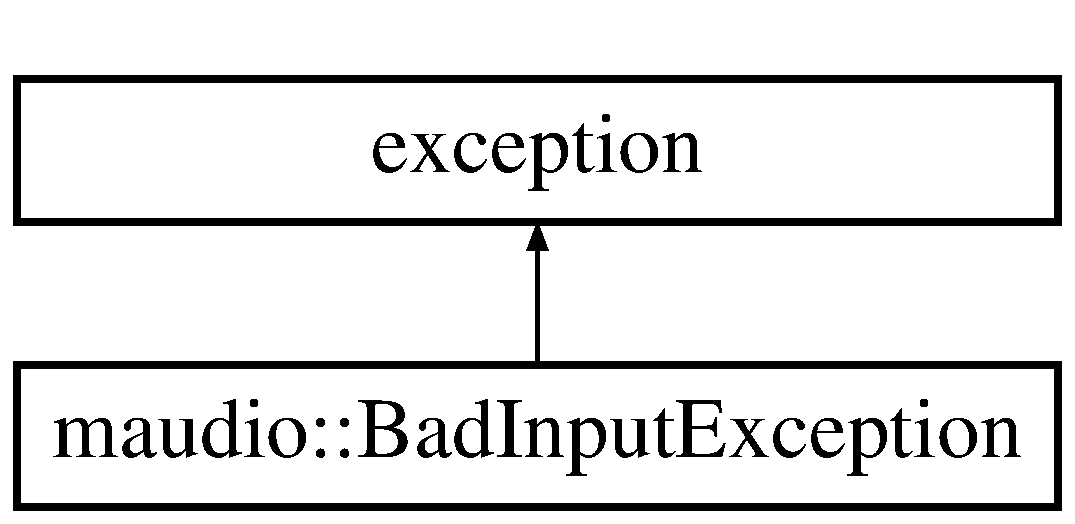
\includegraphics[height=2.000000cm]{classmaudio_1_1BadInputException}
\end{center}
\end{figure}
\subsection*{Public Member Functions}
\begin{DoxyCompactItemize}
\item 
virtual const char $\ast$ \hyperlink{classmaudio_1_1BadInputException_aa783a90827c261838cce43d748dccf05}{what} () const   throw ()
\end{DoxyCompactItemize}


\subsection{Member Function Documentation}
\hypertarget{classmaudio_1_1BadInputException_aa783a90827c261838cce43d748dccf05}{\index{maudio\-::\-Bad\-Input\-Exception@{maudio\-::\-Bad\-Input\-Exception}!what@{what}}
\index{what@{what}!maudio::BadInputException@{maudio\-::\-Bad\-Input\-Exception}}
\subsubsection[{what}]{\setlength{\rightskip}{0pt plus 5cm}virtual const char$\ast$ maudio\-::\-Bad\-Input\-Exception\-::what (
\begin{DoxyParamCaption}
{}
\end{DoxyParamCaption}
) const throw  ) \hspace{0.3cm}{\ttfamily [inline]}, {\ttfamily [virtual]}}}\label{classmaudio_1_1BadInputException_aa783a90827c261838cce43d748dccf05}


The documentation for this class was generated from the following file\-:\begin{DoxyCompactItemize}
\item 
/home/mars/\-Projekte/maudio/src/plugins/include/core/util/\hyperlink{AudioException_8hpp}{Audio\-Exception.\-hpp}\end{DoxyCompactItemize}

\hypertarget{classmaudio_1_1BadOutputException}{\section{maudio\-:\-:Bad\-Output\-Exception Class Reference}
\label{classmaudio_1_1BadOutputException}\index{maudio\-::\-Bad\-Output\-Exception@{maudio\-::\-Bad\-Output\-Exception}}
}


{\ttfamily \#include $<$Audio\-Exception.\-hpp$>$}

Inheritance diagram for maudio\-:\-:Bad\-Output\-Exception\-:\begin{figure}[H]
\begin{center}
\leavevmode
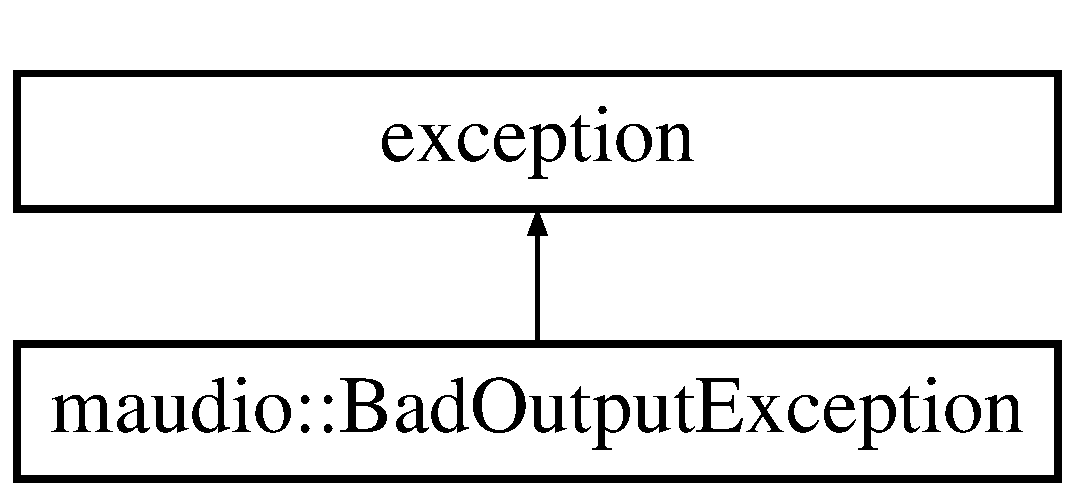
\includegraphics[height=2.000000cm]{classmaudio_1_1BadOutputException}
\end{center}
\end{figure}
\subsection*{Public Member Functions}
\begin{DoxyCompactItemize}
\item 
virtual const char $\ast$ \hyperlink{classmaudio_1_1BadOutputException_ab3d2eda2e4b040716dffa21a61a402b3}{what} () const   throw ()
\end{DoxyCompactItemize}


\subsection{Member Function Documentation}
\hypertarget{classmaudio_1_1BadOutputException_ab3d2eda2e4b040716dffa21a61a402b3}{\index{maudio\-::\-Bad\-Output\-Exception@{maudio\-::\-Bad\-Output\-Exception}!what@{what}}
\index{what@{what}!maudio::BadOutputException@{maudio\-::\-Bad\-Output\-Exception}}
\subsubsection[{what}]{\setlength{\rightskip}{0pt plus 5cm}virtual const char$\ast$ maudio\-::\-Bad\-Output\-Exception\-::what (
\begin{DoxyParamCaption}
{}
\end{DoxyParamCaption}
) const throw  ) \hspace{0.3cm}{\ttfamily [inline]}, {\ttfamily [virtual]}}}\label{classmaudio_1_1BadOutputException_ab3d2eda2e4b040716dffa21a61a402b3}


The documentation for this class was generated from the following file\-:\begin{DoxyCompactItemize}
\item 
/home/mars/\-Projekte/maudio/src/plugins/include/core/util/\hyperlink{AudioException_8hpp}{Audio\-Exception.\-hpp}\end{DoxyCompactItemize}

\hypertarget{classmaudio_1_1BaseAction}{\section{maudio\-:\-:Base\-Action Class Reference}
\label{classmaudio_1_1BaseAction}\index{maudio\-::\-Base\-Action@{maudio\-::\-Base\-Action}}
}


{\ttfamily \#include $<$Base\-Action.\-hpp$>$}

Inheritance diagram for maudio\-:\-:Base\-Action\-:\begin{figure}[H]
\begin{center}
\leavevmode
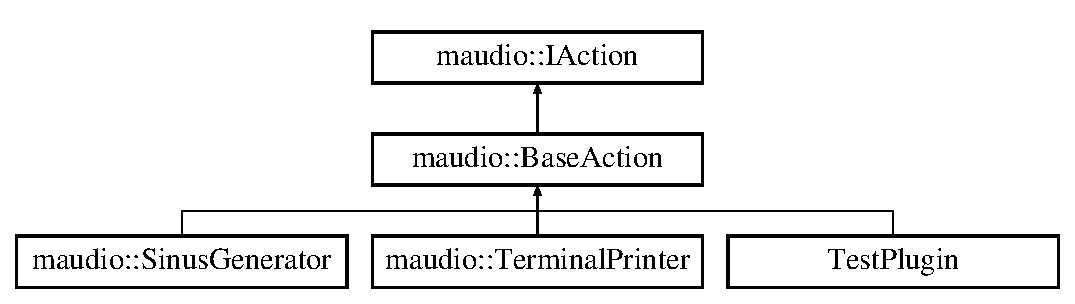
\includegraphics[height=3.000000cm]{classmaudio_1_1BaseAction}
\end{center}
\end{figure}
\subsection*{Public Member Functions}
\begin{DoxyCompactItemize}
\item 
virtual \hyperlink{classmaudio_1_1BaseAction_a98e6cd7921c24d73bf561dfabff89838}{$\sim$\-Base\-Action} ()
\item 
virtual void \hyperlink{classmaudio_1_1BaseAction_a2c5422376581a5d01873833516858753}{delete\-Buffer} (\hyperlink{classmaudio_1_1IAudioBuffer}{I\-Audio\-Buffer} $\ast$data) noexceptfinal
\item 
virtual void \hyperlink{classmaudio_1_1BaseAction_ade1df46a9e5edc1931f3c061f3d51402}{delete\-Info} (\hyperlink{classmaudio_1_1IAudioInfo}{I\-Audio\-Info} $\ast$data) noexceptfinal
\item 
virtual void \hyperlink{classmaudio_1_1BaseAction_a4c1f3d0c024bbdff115ac261bbf1a32c}{delete\-Sample} (\hyperlink{classmaudio_1_1ISample}{I\-Sample} $\ast$data) noexceptfinal
\item 
virtual void \hyperlink{classmaudio_1_1BaseAction_a0e3fe3ae02cdf315fd63944d46419e6e}{add\-Socket} (\hyperlink{classmaudio_1_1ISocket}{I\-Socket} $\ast$socket, int slot) final
\item 
virtual void \hyperlink{classmaudio_1_1BaseAction_aac97bab055f68c49941dbaae9a1ff497}{remove\-Socket} (int slot) final
\item 
virtual int \hyperlink{classmaudio_1_1BaseAction_a25f6c6801b1643bdc0a2bc9bb3534654}{Num\-Inputs} () const final
\item 
virtual \hyperlink{classmaudio_1_1IPropertyManager}{I\-Property\-Manager} $\ast$ \hyperlink{classmaudio_1_1BaseAction_ada21aa4734308191a32a9a2fe1dd4e3d}{get\-Properties} () final
\item 
virtual \hyperlink{classmaudio_1_1IControl}{I\-Control} $\ast$ \hyperlink{classmaudio_1_1BaseAction_a0ecc4f8e47f52d90b0ba7fe2757efe2c}{get\-Control} ()
\end{DoxyCompactItemize}
\subsection*{Protected Attributes}
\begin{DoxyCompactItemize}
\item 
\hyperlink{classmaudio_1_1PropertyManager}{Property\-Manager} \hyperlink{classmaudio_1_1BaseAction_aa18f5dd6b2eb4a522d16df7504494fc3}{m\-Properties}
\item 
std\-::vector$<$ \hyperlink{classmaudio_1_1ISocket}{I\-Socket} $\ast$ $>$ \hyperlink{classmaudio_1_1BaseAction_a5dcde95867364f67871b4f24418d2b00}{m\-Inputs}
\end{DoxyCompactItemize}


\subsection{Constructor \& Destructor Documentation}
\hypertarget{classmaudio_1_1BaseAction_a98e6cd7921c24d73bf561dfabff89838}{\index{maudio\-::\-Base\-Action@{maudio\-::\-Base\-Action}!$\sim$\-Base\-Action@{$\sim$\-Base\-Action}}
\index{$\sim$\-Base\-Action@{$\sim$\-Base\-Action}!maudio::BaseAction@{maudio\-::\-Base\-Action}}
\subsubsection[{$\sim$\-Base\-Action}]{\setlength{\rightskip}{0pt plus 5cm}maudio\-::\-Base\-Action\-::$\sim$\-Base\-Action (
\begin{DoxyParamCaption}
{}
\end{DoxyParamCaption}
)\hspace{0.3cm}{\ttfamily [virtual]}}}\label{classmaudio_1_1BaseAction_a98e6cd7921c24d73bf561dfabff89838}


\subsection{Member Function Documentation}
\hypertarget{classmaudio_1_1BaseAction_a0e3fe3ae02cdf315fd63944d46419e6e}{\index{maudio\-::\-Base\-Action@{maudio\-::\-Base\-Action}!add\-Socket@{add\-Socket}}
\index{add\-Socket@{add\-Socket}!maudio::BaseAction@{maudio\-::\-Base\-Action}}
\subsubsection[{add\-Socket}]{\setlength{\rightskip}{0pt plus 5cm}void maudio\-::\-Base\-Action\-::add\-Socket (
\begin{DoxyParamCaption}
\item[{{\bf I\-Socket} $\ast$}]{socket, }
\item[{int}]{slot}
\end{DoxyParamCaption}
)\hspace{0.3cm}{\ttfamily [final]}, {\ttfamily [virtual]}}}\label{classmaudio_1_1BaseAction_a0e3fe3ae02cdf315fd63944d46419e6e}


Implements \hyperlink{classmaudio_1_1IAction_a0dac443df118fafeb020d2254d3c8c8a}{maudio\-::\-I\-Action}.

\hypertarget{classmaudio_1_1BaseAction_a2c5422376581a5d01873833516858753}{\index{maudio\-::\-Base\-Action@{maudio\-::\-Base\-Action}!delete\-Buffer@{delete\-Buffer}}
\index{delete\-Buffer@{delete\-Buffer}!maudio::BaseAction@{maudio\-::\-Base\-Action}}
\subsubsection[{delete\-Buffer}]{\setlength{\rightskip}{0pt plus 5cm}void maudio\-::\-Base\-Action\-::delete\-Buffer (
\begin{DoxyParamCaption}
\item[{{\bf I\-Audio\-Buffer} $\ast$}]{data}
\end{DoxyParamCaption}
)\hspace{0.3cm}{\ttfamily [final]}, {\ttfamily [virtual]}, {\ttfamily [noexcept]}}}\label{classmaudio_1_1BaseAction_a2c5422376581a5d01873833516858753}


Implements \hyperlink{classmaudio_1_1IAction_a6be8c626cd3043c4114d9cf998fd0388}{maudio\-::\-I\-Action}.

\hypertarget{classmaudio_1_1BaseAction_ade1df46a9e5edc1931f3c061f3d51402}{\index{maudio\-::\-Base\-Action@{maudio\-::\-Base\-Action}!delete\-Info@{delete\-Info}}
\index{delete\-Info@{delete\-Info}!maudio::BaseAction@{maudio\-::\-Base\-Action}}
\subsubsection[{delete\-Info}]{\setlength{\rightskip}{0pt plus 5cm}void maudio\-::\-Base\-Action\-::delete\-Info (
\begin{DoxyParamCaption}
\item[{{\bf I\-Audio\-Info} $\ast$}]{data}
\end{DoxyParamCaption}
)\hspace{0.3cm}{\ttfamily [final]}, {\ttfamily [virtual]}, {\ttfamily [noexcept]}}}\label{classmaudio_1_1BaseAction_ade1df46a9e5edc1931f3c061f3d51402}


Implements \hyperlink{classmaudio_1_1IAction_af02a219faa2361dd14759e1e92003d33}{maudio\-::\-I\-Action}.

\hypertarget{classmaudio_1_1BaseAction_a4c1f3d0c024bbdff115ac261bbf1a32c}{\index{maudio\-::\-Base\-Action@{maudio\-::\-Base\-Action}!delete\-Sample@{delete\-Sample}}
\index{delete\-Sample@{delete\-Sample}!maudio::BaseAction@{maudio\-::\-Base\-Action}}
\subsubsection[{delete\-Sample}]{\setlength{\rightskip}{0pt plus 5cm}void maudio\-::\-Base\-Action\-::delete\-Sample (
\begin{DoxyParamCaption}
\item[{{\bf I\-Sample} $\ast$}]{data}
\end{DoxyParamCaption}
)\hspace{0.3cm}{\ttfamily [final]}, {\ttfamily [virtual]}, {\ttfamily [noexcept]}}}\label{classmaudio_1_1BaseAction_a4c1f3d0c024bbdff115ac261bbf1a32c}


Implements \hyperlink{classmaudio_1_1IAction_ae4bdc7487e1229ded107ff8d42275bd3}{maudio\-::\-I\-Action}.

\hypertarget{classmaudio_1_1BaseAction_a0ecc4f8e47f52d90b0ba7fe2757efe2c}{\index{maudio\-::\-Base\-Action@{maudio\-::\-Base\-Action}!get\-Control@{get\-Control}}
\index{get\-Control@{get\-Control}!maudio::BaseAction@{maudio\-::\-Base\-Action}}
\subsubsection[{get\-Control}]{\setlength{\rightskip}{0pt plus 5cm}{\bf I\-Control} $\ast$ maudio\-::\-Base\-Action\-::get\-Control (
\begin{DoxyParamCaption}
{}
\end{DoxyParamCaption}
)\hspace{0.3cm}{\ttfamily [virtual]}}}\label{classmaudio_1_1BaseAction_a0ecc4f8e47f52d90b0ba7fe2757efe2c}


Implements \hyperlink{classmaudio_1_1IAction_a0103686135171d24dc7901a81ae77ace}{maudio\-::\-I\-Action}.



Reimplemented in \hyperlink{classmaudio_1_1TerminalPrinter_acef99a9118ebb6908166d8e97e7bb3e9}{maudio\-::\-Terminal\-Printer}.

\hypertarget{classmaudio_1_1BaseAction_ada21aa4734308191a32a9a2fe1dd4e3d}{\index{maudio\-::\-Base\-Action@{maudio\-::\-Base\-Action}!get\-Properties@{get\-Properties}}
\index{get\-Properties@{get\-Properties}!maudio::BaseAction@{maudio\-::\-Base\-Action}}
\subsubsection[{get\-Properties}]{\setlength{\rightskip}{0pt plus 5cm}{\bf I\-Property\-Manager} $\ast$ maudio\-::\-Base\-Action\-::get\-Properties (
\begin{DoxyParamCaption}
{}
\end{DoxyParamCaption}
)\hspace{0.3cm}{\ttfamily [final]}, {\ttfamily [virtual]}}}\label{classmaudio_1_1BaseAction_ada21aa4734308191a32a9a2fe1dd4e3d}


Implements \hyperlink{classmaudio_1_1IAction_a59edeb0de77724d42bc51e9b7f7b6d41}{maudio\-::\-I\-Action}.

\hypertarget{classmaudio_1_1BaseAction_a25f6c6801b1643bdc0a2bc9bb3534654}{\index{maudio\-::\-Base\-Action@{maudio\-::\-Base\-Action}!Num\-Inputs@{Num\-Inputs}}
\index{Num\-Inputs@{Num\-Inputs}!maudio::BaseAction@{maudio\-::\-Base\-Action}}
\subsubsection[{Num\-Inputs}]{\setlength{\rightskip}{0pt plus 5cm}int maudio\-::\-Base\-Action\-::\-Num\-Inputs (
\begin{DoxyParamCaption}
{}
\end{DoxyParamCaption}
) const\hspace{0.3cm}{\ttfamily [final]}, {\ttfamily [virtual]}}}\label{classmaudio_1_1BaseAction_a25f6c6801b1643bdc0a2bc9bb3534654}


Implements \hyperlink{classmaudio_1_1IAction_ad850f2f577a12e41c71994479773079f}{maudio\-::\-I\-Action}.

\hypertarget{classmaudio_1_1BaseAction_aac97bab055f68c49941dbaae9a1ff497}{\index{maudio\-::\-Base\-Action@{maudio\-::\-Base\-Action}!remove\-Socket@{remove\-Socket}}
\index{remove\-Socket@{remove\-Socket}!maudio::BaseAction@{maudio\-::\-Base\-Action}}
\subsubsection[{remove\-Socket}]{\setlength{\rightskip}{0pt plus 5cm}void maudio\-::\-Base\-Action\-::remove\-Socket (
\begin{DoxyParamCaption}
\item[{int}]{slot}
\end{DoxyParamCaption}
)\hspace{0.3cm}{\ttfamily [final]}, {\ttfamily [virtual]}}}\label{classmaudio_1_1BaseAction_aac97bab055f68c49941dbaae9a1ff497}


Implements \hyperlink{classmaudio_1_1IAction_aa562ad351f4923aeef7d8a7c0450d74e}{maudio\-::\-I\-Action}.



\subsection{Member Data Documentation}
\hypertarget{classmaudio_1_1BaseAction_a5dcde95867364f67871b4f24418d2b00}{\index{maudio\-::\-Base\-Action@{maudio\-::\-Base\-Action}!m\-Inputs@{m\-Inputs}}
\index{m\-Inputs@{m\-Inputs}!maudio::BaseAction@{maudio\-::\-Base\-Action}}
\subsubsection[{m\-Inputs}]{\setlength{\rightskip}{0pt plus 5cm}std\-::vector$<${\bf I\-Socket} $\ast$$>$ maudio\-::\-Base\-Action\-::m\-Inputs\hspace{0.3cm}{\ttfamily [protected]}}}\label{classmaudio_1_1BaseAction_a5dcde95867364f67871b4f24418d2b00}
\hypertarget{classmaudio_1_1BaseAction_aa18f5dd6b2eb4a522d16df7504494fc3}{\index{maudio\-::\-Base\-Action@{maudio\-::\-Base\-Action}!m\-Properties@{m\-Properties}}
\index{m\-Properties@{m\-Properties}!maudio::BaseAction@{maudio\-::\-Base\-Action}}
\subsubsection[{m\-Properties}]{\setlength{\rightskip}{0pt plus 5cm}{\bf Property\-Manager} maudio\-::\-Base\-Action\-::m\-Properties\hspace{0.3cm}{\ttfamily [protected]}}}\label{classmaudio_1_1BaseAction_aa18f5dd6b2eb4a522d16df7504494fc3}


The documentation for this class was generated from the following files\-:\begin{DoxyCompactItemize}
\item 
/home/mars/\-Projekte/maudio/src/plugins/include/core/actions/\hyperlink{BaseAction_8hpp}{Base\-Action.\-hpp}\item 
/home/mars/\-Projekte/maudio/src/core/actions/\hyperlink{core_2actions_2BaseAction_8cpp}{Base\-Action.\-cpp}\end{DoxyCompactItemize}

\hypertarget{classmaudio_1_1ChannelsException}{\section{maudio\-:\-:Channels\-Exception Class Reference}
\label{classmaudio_1_1ChannelsException}\index{maudio\-::\-Channels\-Exception@{maudio\-::\-Channels\-Exception}}
}


{\ttfamily \#include $<$Audio\-Exception.\-hpp$>$}

Inheritance diagram for maudio\-:\-:Channels\-Exception\-:\begin{figure}[H]
\begin{center}
\leavevmode
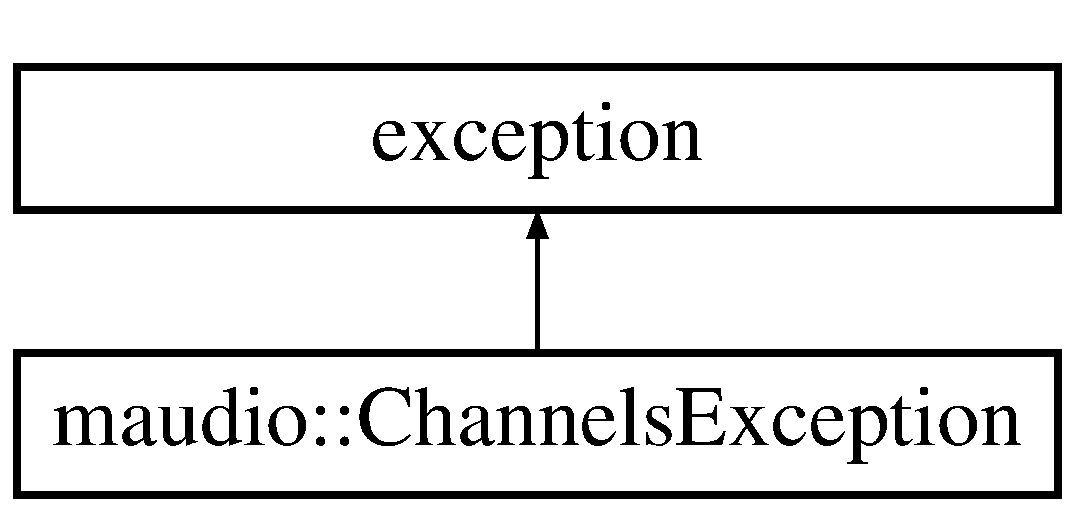
\includegraphics[height=2.000000cm]{classmaudio_1_1ChannelsException}
\end{center}
\end{figure}
\subsection*{Public Member Functions}
\begin{DoxyCompactItemize}
\item 
virtual const char $\ast$ \hyperlink{classmaudio_1_1ChannelsException_a51e467115efd731eaaf8e0c59f3d526b}{what} () const   throw ()
\end{DoxyCompactItemize}


\subsection{Member Function Documentation}
\hypertarget{classmaudio_1_1ChannelsException_a51e467115efd731eaaf8e0c59f3d526b}{\index{maudio\-::\-Channels\-Exception@{maudio\-::\-Channels\-Exception}!what@{what}}
\index{what@{what}!maudio::ChannelsException@{maudio\-::\-Channels\-Exception}}
\subsubsection[{what}]{\setlength{\rightskip}{0pt plus 5cm}virtual const char$\ast$ maudio\-::\-Channels\-Exception\-::what (
\begin{DoxyParamCaption}
{}
\end{DoxyParamCaption}
) const throw  ) \hspace{0.3cm}{\ttfamily [inline]}, {\ttfamily [virtual]}}}\label{classmaudio_1_1ChannelsException_a51e467115efd731eaaf8e0c59f3d526b}


The documentation for this class was generated from the following file\-:\begin{DoxyCompactItemize}
\item 
/home/mars/\-Projekte/maudio/src/plugins/include/core/util/\hyperlink{AudioException_8hpp}{Audio\-Exception.\-hpp}\end{DoxyCompactItemize}

\hypertarget{classmaudio_1_1CircleException}{\section{maudio\-:\-:Circle\-Exception Class Reference}
\label{classmaudio_1_1CircleException}\index{maudio\-::\-Circle\-Exception@{maudio\-::\-Circle\-Exception}}
}


{\ttfamily \#include $<$Audio\-Exception.\-hpp$>$}

Inheritance diagram for maudio\-:\-:Circle\-Exception\-:\begin{figure}[H]
\begin{center}
\leavevmode
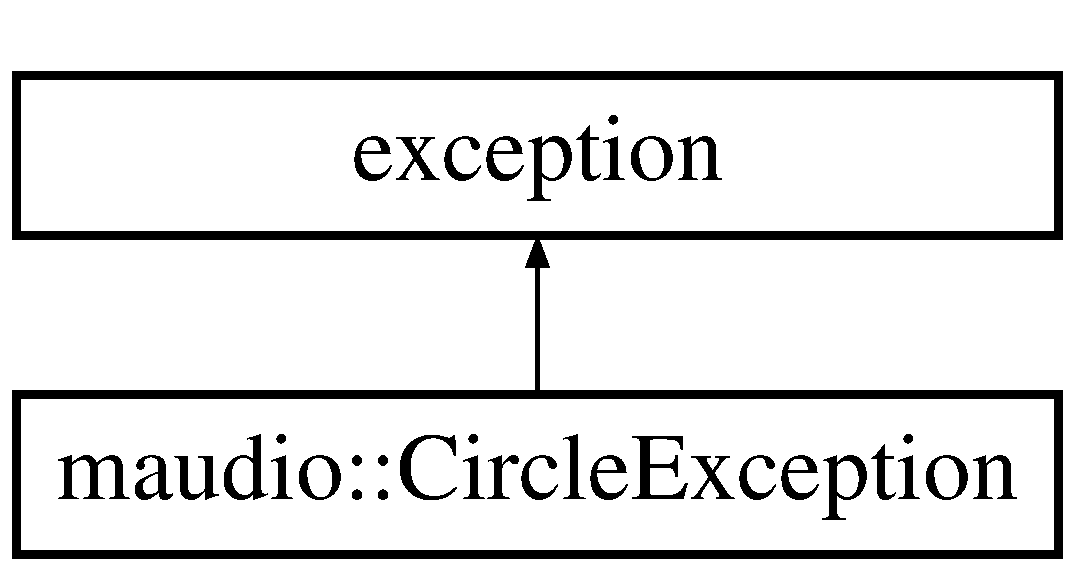
\includegraphics[height=2.000000cm]{classmaudio_1_1CircleException}
\end{center}
\end{figure}
\subsection*{Public Member Functions}
\begin{DoxyCompactItemize}
\item 
virtual const char $\ast$ \hyperlink{classmaudio_1_1CircleException_ab5519a875749b19933ac5a3130d572ad}{what} () const   throw ()
\end{DoxyCompactItemize}


\subsection{Member Function Documentation}
\hypertarget{classmaudio_1_1CircleException_ab5519a875749b19933ac5a3130d572ad}{\index{maudio\-::\-Circle\-Exception@{maudio\-::\-Circle\-Exception}!what@{what}}
\index{what@{what}!maudio::CircleException@{maudio\-::\-Circle\-Exception}}
\subsubsection[{what}]{\setlength{\rightskip}{0pt plus 5cm}virtual const char$\ast$ maudio\-::\-Circle\-Exception\-::what (
\begin{DoxyParamCaption}
{}
\end{DoxyParamCaption}
) const throw  ) \hspace{0.3cm}{\ttfamily [inline]}, {\ttfamily [virtual]}}}\label{classmaudio_1_1CircleException_ab5519a875749b19933ac5a3130d572ad}


The documentation for this class was generated from the following file\-:\begin{DoxyCompactItemize}
\item 
/home/mars/\-Projekte/maudio/src/plugins/include/core/util/\hyperlink{AudioException_8hpp}{Audio\-Exception.\-hpp}\end{DoxyCompactItemize}

\hypertarget{classmaudio_1_1Config}{\section{maudio\-:\-:Config Class Reference}
\label{classmaudio_1_1Config}\index{maudio\-::\-Config@{maudio\-::\-Config}}
}


{\ttfamily \#include $<$Config.\-hpp$>$}

Inheritance diagram for maudio\-:\-:Config\-:\begin{figure}[H]
\begin{center}
\leavevmode
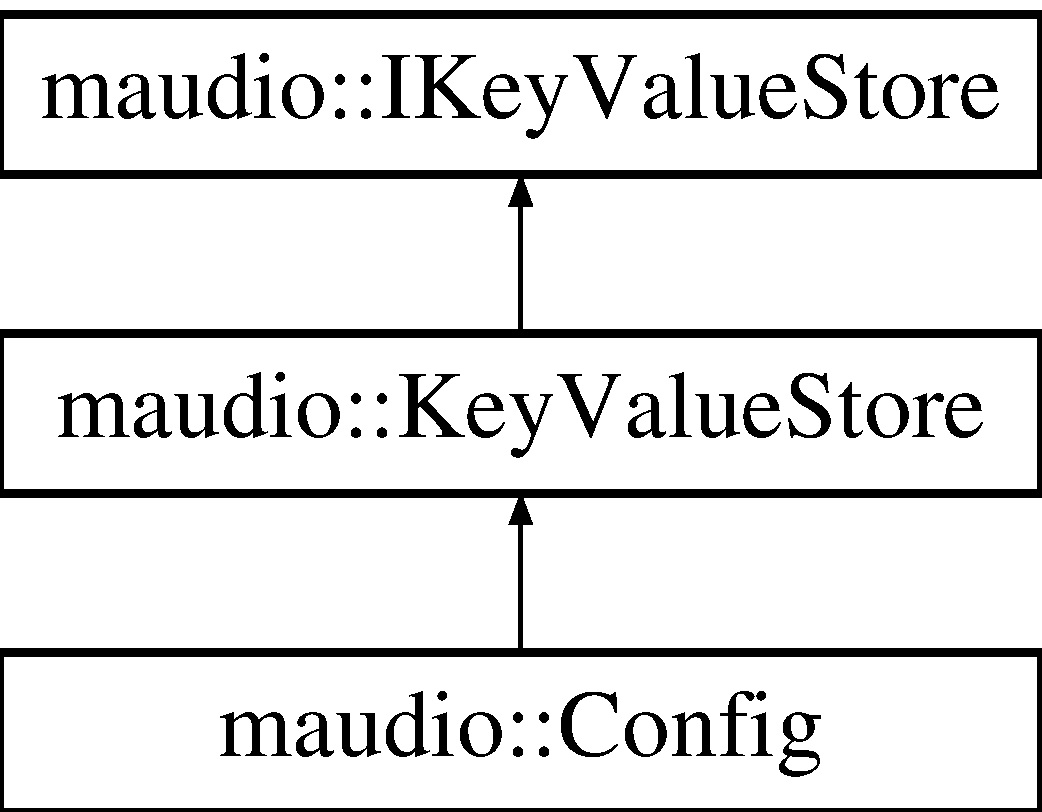
\includegraphics[height=3.000000cm]{classmaudio_1_1Config}
\end{center}
\end{figure}
\subsection*{Public Member Functions}
\begin{DoxyCompactItemize}
\item 
\hyperlink{classmaudio_1_1Config_a78661d78939a884924df4ec3f5af231d}{Config} ()
\item 
\hyperlink{classmaudio_1_1Config_a0abf7bbadd66770632a039bef0cb601a}{$\sim$\-Config} ()
\item 
void \hyperlink{classmaudio_1_1Config_aaa1bfe731a0058dc753cb7edcf048000}{parse\-File} (const std\-::string \&file)
\item 
void \hyperlink{classmaudio_1_1Config_ac30d2dbbee2fdbb63e812a5077eda0ee}{save\-File} () const 
\item 
void \hyperlink{classmaudio_1_1Config_a561024ce11c4b385afe2d7463bdd4d7a}{save\-File} (const std\-::string \&file) const 
\item 
void \hyperlink{classmaudio_1_1Config_aed5be396535c3c85176eea3fc892c0ed}{set\-Defaults} ()
\end{DoxyCompactItemize}
\subsection*{Additional Inherited Members}


\subsection{Constructor \& Destructor Documentation}
\hypertarget{classmaudio_1_1Config_a78661d78939a884924df4ec3f5af231d}{\index{maudio\-::\-Config@{maudio\-::\-Config}!Config@{Config}}
\index{Config@{Config}!maudio::Config@{maudio\-::\-Config}}
\subsubsection[{Config}]{\setlength{\rightskip}{0pt plus 5cm}maudio\-::\-Config\-::\-Config (
\begin{DoxyParamCaption}
{}
\end{DoxyParamCaption}
)}}\label{classmaudio_1_1Config_a78661d78939a884924df4ec3f5af231d}
\hypertarget{classmaudio_1_1Config_a0abf7bbadd66770632a039bef0cb601a}{\index{maudio\-::\-Config@{maudio\-::\-Config}!$\sim$\-Config@{$\sim$\-Config}}
\index{$\sim$\-Config@{$\sim$\-Config}!maudio::Config@{maudio\-::\-Config}}
\subsubsection[{$\sim$\-Config}]{\setlength{\rightskip}{0pt plus 5cm}maudio\-::\-Config\-::$\sim$\-Config (
\begin{DoxyParamCaption}
{}
\end{DoxyParamCaption}
)}}\label{classmaudio_1_1Config_a0abf7bbadd66770632a039bef0cb601a}


\subsection{Member Function Documentation}
\hypertarget{classmaudio_1_1Config_aaa1bfe731a0058dc753cb7edcf048000}{\index{maudio\-::\-Config@{maudio\-::\-Config}!parse\-File@{parse\-File}}
\index{parse\-File@{parse\-File}!maudio::Config@{maudio\-::\-Config}}
\subsubsection[{parse\-File}]{\setlength{\rightskip}{0pt plus 5cm}void maudio\-::\-Config\-::parse\-File (
\begin{DoxyParamCaption}
\item[{const std\-::string \&}]{file}
\end{DoxyParamCaption}
)}}\label{classmaudio_1_1Config_aaa1bfe731a0058dc753cb7edcf048000}
\hypertarget{classmaudio_1_1Config_ac30d2dbbee2fdbb63e812a5077eda0ee}{\index{maudio\-::\-Config@{maudio\-::\-Config}!save\-File@{save\-File}}
\index{save\-File@{save\-File}!maudio::Config@{maudio\-::\-Config}}
\subsubsection[{save\-File}]{\setlength{\rightskip}{0pt plus 5cm}void maudio\-::\-Config\-::save\-File (
\begin{DoxyParamCaption}
{}
\end{DoxyParamCaption}
) const}}\label{classmaudio_1_1Config_ac30d2dbbee2fdbb63e812a5077eda0ee}
\hypertarget{classmaudio_1_1Config_a561024ce11c4b385afe2d7463bdd4d7a}{\index{maudio\-::\-Config@{maudio\-::\-Config}!save\-File@{save\-File}}
\index{save\-File@{save\-File}!maudio::Config@{maudio\-::\-Config}}
\subsubsection[{save\-File}]{\setlength{\rightskip}{0pt plus 5cm}void maudio\-::\-Config\-::save\-File (
\begin{DoxyParamCaption}
\item[{const std\-::string \&}]{file}
\end{DoxyParamCaption}
) const}}\label{classmaudio_1_1Config_a561024ce11c4b385afe2d7463bdd4d7a}
\hypertarget{classmaudio_1_1Config_aed5be396535c3c85176eea3fc892c0ed}{\index{maudio\-::\-Config@{maudio\-::\-Config}!set\-Defaults@{set\-Defaults}}
\index{set\-Defaults@{set\-Defaults}!maudio::Config@{maudio\-::\-Config}}
\subsubsection[{set\-Defaults}]{\setlength{\rightskip}{0pt plus 5cm}void maudio\-::\-Config\-::set\-Defaults (
\begin{DoxyParamCaption}
{}
\end{DoxyParamCaption}
)}}\label{classmaudio_1_1Config_aed5be396535c3c85176eea3fc892c0ed}


The documentation for this class was generated from the following files\-:\begin{DoxyCompactItemize}
\item 
/home/mars/\-Projekte/maudio/src/plugins/include/core/store/\hyperlink{Config_8hpp}{Config.\-hpp}\item 
/home/mars/\-Projekte/maudio/src/core/store/\hyperlink{core_2store_2Config_8cpp}{Config.\-cpp}\end{DoxyCompactItemize}

\hypertarget{classmaudio_1_1ConfigManager}{\section{maudio\-:\-:Config\-Manager Class Reference}
\label{classmaudio_1_1ConfigManager}\index{maudio\-::\-Config\-Manager@{maudio\-::\-Config\-Manager}}
}


{\ttfamily \#include $<$Config\-Manager.\-hpp$>$}

\subsection*{Public Member Functions}
\begin{DoxyCompactItemize}
\item 
void \hyperlink{classmaudio_1_1ConfigManager_ad05c11aa043d94d1738a1f2800c89120}{set\-Config\-Path} (const std\-::string \&path)
\item 
std\-::string \hyperlink{classmaudio_1_1ConfigManager_ad4a53c6161d1a6053b4cbaa1a941d925}{get\-Config\-Path} () const 
\item 
const \hyperlink{classmaudio_1_1Config}{Config} \& \hyperlink{classmaudio_1_1ConfigManager_abe3f974a561904a6f8bac751e74941b0}{get\-Config} () const 
\item 
\hyperlink{classmaudio_1_1Config}{Config} \& \hyperlink{classmaudio_1_1ConfigManager_a332e953e5007f47943395e164840acbe}{manipulate} ()
\end{DoxyCompactItemize}
\subsection*{Static Public Member Functions}
\begin{DoxyCompactItemize}
\item 
static \hyperlink{classmaudio_1_1ConfigManager}{Config\-Manager} $\ast$ \hyperlink{classmaudio_1_1ConfigManager_a8c673f65be30141b3724cefff0fef5b1}{Instance} ()
\end{DoxyCompactItemize}


\subsection{Member Function Documentation}
\hypertarget{classmaudio_1_1ConfigManager_abe3f974a561904a6f8bac751e74941b0}{\index{maudio\-::\-Config\-Manager@{maudio\-::\-Config\-Manager}!get\-Config@{get\-Config}}
\index{get\-Config@{get\-Config}!maudio::ConfigManager@{maudio\-::\-Config\-Manager}}
\subsubsection[{get\-Config}]{\setlength{\rightskip}{0pt plus 5cm}const {\bf Config} \& maudio\-::\-Config\-Manager\-::get\-Config (
\begin{DoxyParamCaption}
{}
\end{DoxyParamCaption}
) const}}\label{classmaudio_1_1ConfigManager_abe3f974a561904a6f8bac751e74941b0}
\hypertarget{classmaudio_1_1ConfigManager_ad4a53c6161d1a6053b4cbaa1a941d925}{\index{maudio\-::\-Config\-Manager@{maudio\-::\-Config\-Manager}!get\-Config\-Path@{get\-Config\-Path}}
\index{get\-Config\-Path@{get\-Config\-Path}!maudio::ConfigManager@{maudio\-::\-Config\-Manager}}
\subsubsection[{get\-Config\-Path}]{\setlength{\rightskip}{0pt plus 5cm}std\-::string maudio\-::\-Config\-Manager\-::get\-Config\-Path (
\begin{DoxyParamCaption}
{}
\end{DoxyParamCaption}
) const}}\label{classmaudio_1_1ConfigManager_ad4a53c6161d1a6053b4cbaa1a941d925}
\hypertarget{classmaudio_1_1ConfigManager_a8c673f65be30141b3724cefff0fef5b1}{\index{maudio\-::\-Config\-Manager@{maudio\-::\-Config\-Manager}!Instance@{Instance}}
\index{Instance@{Instance}!maudio::ConfigManager@{maudio\-::\-Config\-Manager}}
\subsubsection[{Instance}]{\setlength{\rightskip}{0pt plus 5cm}{\bf Config\-Manager} $\ast$ maudio\-::\-Config\-Manager\-::\-Instance (
\begin{DoxyParamCaption}
{}
\end{DoxyParamCaption}
)\hspace{0.3cm}{\ttfamily [static]}}}\label{classmaudio_1_1ConfigManager_a8c673f65be30141b3724cefff0fef5b1}
\hypertarget{classmaudio_1_1ConfigManager_a332e953e5007f47943395e164840acbe}{\index{maudio\-::\-Config\-Manager@{maudio\-::\-Config\-Manager}!manipulate@{manipulate}}
\index{manipulate@{manipulate}!maudio::ConfigManager@{maudio\-::\-Config\-Manager}}
\subsubsection[{manipulate}]{\setlength{\rightskip}{0pt plus 5cm}{\bf Config} \& maudio\-::\-Config\-Manager\-::manipulate (
\begin{DoxyParamCaption}
{}
\end{DoxyParamCaption}
)}}\label{classmaudio_1_1ConfigManager_a332e953e5007f47943395e164840acbe}
\hypertarget{classmaudio_1_1ConfigManager_ad05c11aa043d94d1738a1f2800c89120}{\index{maudio\-::\-Config\-Manager@{maudio\-::\-Config\-Manager}!set\-Config\-Path@{set\-Config\-Path}}
\index{set\-Config\-Path@{set\-Config\-Path}!maudio::ConfigManager@{maudio\-::\-Config\-Manager}}
\subsubsection[{set\-Config\-Path}]{\setlength{\rightskip}{0pt plus 5cm}void maudio\-::\-Config\-Manager\-::set\-Config\-Path (
\begin{DoxyParamCaption}
\item[{const std\-::string \&}]{path}
\end{DoxyParamCaption}
)}}\label{classmaudio_1_1ConfigManager_ad05c11aa043d94d1738a1f2800c89120}


The documentation for this class was generated from the following files\-:\begin{DoxyCompactItemize}
\item 
/home/mars/\-Projekte/maudio/src/plugins/include/core/store/\hyperlink{ConfigManager_8hpp}{Config\-Manager.\-hpp}\item 
/home/mars/\-Projekte/maudio/src/core/store/\hyperlink{core_2store_2ConfigManager_8cpp}{Config\-Manager.\-cpp}\end{DoxyCompactItemize}

\hypertarget{classmaudio_1_1FileInfo}{\section{maudio\-:\-:File\-Info Class Reference}
\label{classmaudio_1_1FileInfo}\index{maudio\-::\-File\-Info@{maudio\-::\-File\-Info}}
}


{\ttfamily \#include $<$File\-Info.\-hpp$>$}

\subsection*{Public Attributes}
\begin{DoxyCompactItemize}
\item 
std\-::string \hyperlink{classmaudio_1_1FileInfo_af6ae1285091042123f8a085e8409519a}{File\-Name}
\item 
std\-::string \hyperlink{classmaudio_1_1FileInfo_a75de1fe16dda2fa2b740e5840befa136}{Title}
\item 
std\-::string \hyperlink{classmaudio_1_1FileInfo_a14deaeaf7ce3f6199df91949f9b203fa}{Copyright}
\item 
std\-::string \hyperlink{classmaudio_1_1FileInfo_afcac65260e528fdcfd9edcc03546e050}{Software}
\item 
std\-::string \hyperlink{classmaudio_1_1FileInfo_ac7d8160fd99886cf9965320a6205f8a2}{Artist}
\item 
std\-::string \hyperlink{classmaudio_1_1FileInfo_a261b363a280a559f2798cdd4c68c61b2}{Comment}
\item 
std\-::string \hyperlink{classmaudio_1_1FileInfo_a5e87a7861359ae6561feb6dedd44706f}{Date}
\item 
std\-::string \hyperlink{classmaudio_1_1FileInfo_a7401b31fcb454d8643a52df46f952462}{Album}
\item 
std\-::string \hyperlink{classmaudio_1_1FileInfo_a66338e82866dc97e0e1f4de4b17dd376}{License}
\item 
std\-::string \hyperlink{classmaudio_1_1FileInfo_ad3861dc761b16bf86695827542b4d02d}{Tracknumber}
\item 
std\-::string \hyperlink{classmaudio_1_1FileInfo_a719ece71b50358f453939384bbeced83}{Genre}
\end{DoxyCompactItemize}


\subsection{Member Data Documentation}
\hypertarget{classmaudio_1_1FileInfo_a7401b31fcb454d8643a52df46f952462}{\index{maudio\-::\-File\-Info@{maudio\-::\-File\-Info}!Album@{Album}}
\index{Album@{Album}!maudio::FileInfo@{maudio\-::\-File\-Info}}
\subsubsection[{Album}]{\setlength{\rightskip}{0pt plus 5cm}std\-::string maudio\-::\-File\-Info\-::\-Album}}\label{classmaudio_1_1FileInfo_a7401b31fcb454d8643a52df46f952462}
\hypertarget{classmaudio_1_1FileInfo_ac7d8160fd99886cf9965320a6205f8a2}{\index{maudio\-::\-File\-Info@{maudio\-::\-File\-Info}!Artist@{Artist}}
\index{Artist@{Artist}!maudio::FileInfo@{maudio\-::\-File\-Info}}
\subsubsection[{Artist}]{\setlength{\rightskip}{0pt plus 5cm}std\-::string maudio\-::\-File\-Info\-::\-Artist}}\label{classmaudio_1_1FileInfo_ac7d8160fd99886cf9965320a6205f8a2}
\hypertarget{classmaudio_1_1FileInfo_a261b363a280a559f2798cdd4c68c61b2}{\index{maudio\-::\-File\-Info@{maudio\-::\-File\-Info}!Comment@{Comment}}
\index{Comment@{Comment}!maudio::FileInfo@{maudio\-::\-File\-Info}}
\subsubsection[{Comment}]{\setlength{\rightskip}{0pt plus 5cm}std\-::string maudio\-::\-File\-Info\-::\-Comment}}\label{classmaudio_1_1FileInfo_a261b363a280a559f2798cdd4c68c61b2}
\hypertarget{classmaudio_1_1FileInfo_a14deaeaf7ce3f6199df91949f9b203fa}{\index{maudio\-::\-File\-Info@{maudio\-::\-File\-Info}!Copyright@{Copyright}}
\index{Copyright@{Copyright}!maudio::FileInfo@{maudio\-::\-File\-Info}}
\subsubsection[{Copyright}]{\setlength{\rightskip}{0pt plus 5cm}std\-::string maudio\-::\-File\-Info\-::\-Copyright}}\label{classmaudio_1_1FileInfo_a14deaeaf7ce3f6199df91949f9b203fa}
\hypertarget{classmaudio_1_1FileInfo_a5e87a7861359ae6561feb6dedd44706f}{\index{maudio\-::\-File\-Info@{maudio\-::\-File\-Info}!Date@{Date}}
\index{Date@{Date}!maudio::FileInfo@{maudio\-::\-File\-Info}}
\subsubsection[{Date}]{\setlength{\rightskip}{0pt plus 5cm}std\-::string maudio\-::\-File\-Info\-::\-Date}}\label{classmaudio_1_1FileInfo_a5e87a7861359ae6561feb6dedd44706f}
\hypertarget{classmaudio_1_1FileInfo_af6ae1285091042123f8a085e8409519a}{\index{maudio\-::\-File\-Info@{maudio\-::\-File\-Info}!File\-Name@{File\-Name}}
\index{File\-Name@{File\-Name}!maudio::FileInfo@{maudio\-::\-File\-Info}}
\subsubsection[{File\-Name}]{\setlength{\rightskip}{0pt plus 5cm}std\-::string maudio\-::\-File\-Info\-::\-File\-Name}}\label{classmaudio_1_1FileInfo_af6ae1285091042123f8a085e8409519a}
\hypertarget{classmaudio_1_1FileInfo_a719ece71b50358f453939384bbeced83}{\index{maudio\-::\-File\-Info@{maudio\-::\-File\-Info}!Genre@{Genre}}
\index{Genre@{Genre}!maudio::FileInfo@{maudio\-::\-File\-Info}}
\subsubsection[{Genre}]{\setlength{\rightskip}{0pt plus 5cm}std\-::string maudio\-::\-File\-Info\-::\-Genre}}\label{classmaudio_1_1FileInfo_a719ece71b50358f453939384bbeced83}
\hypertarget{classmaudio_1_1FileInfo_a66338e82866dc97e0e1f4de4b17dd376}{\index{maudio\-::\-File\-Info@{maudio\-::\-File\-Info}!License@{License}}
\index{License@{License}!maudio::FileInfo@{maudio\-::\-File\-Info}}
\subsubsection[{License}]{\setlength{\rightskip}{0pt plus 5cm}std\-::string maudio\-::\-File\-Info\-::\-License}}\label{classmaudio_1_1FileInfo_a66338e82866dc97e0e1f4de4b17dd376}
\hypertarget{classmaudio_1_1FileInfo_afcac65260e528fdcfd9edcc03546e050}{\index{maudio\-::\-File\-Info@{maudio\-::\-File\-Info}!Software@{Software}}
\index{Software@{Software}!maudio::FileInfo@{maudio\-::\-File\-Info}}
\subsubsection[{Software}]{\setlength{\rightskip}{0pt plus 5cm}std\-::string maudio\-::\-File\-Info\-::\-Software}}\label{classmaudio_1_1FileInfo_afcac65260e528fdcfd9edcc03546e050}
\hypertarget{classmaudio_1_1FileInfo_a75de1fe16dda2fa2b740e5840befa136}{\index{maudio\-::\-File\-Info@{maudio\-::\-File\-Info}!Title@{Title}}
\index{Title@{Title}!maudio::FileInfo@{maudio\-::\-File\-Info}}
\subsubsection[{Title}]{\setlength{\rightskip}{0pt plus 5cm}std\-::string maudio\-::\-File\-Info\-::\-Title}}\label{classmaudio_1_1FileInfo_a75de1fe16dda2fa2b740e5840befa136}
\hypertarget{classmaudio_1_1FileInfo_ad3861dc761b16bf86695827542b4d02d}{\index{maudio\-::\-File\-Info@{maudio\-::\-File\-Info}!Tracknumber@{Tracknumber}}
\index{Tracknumber@{Tracknumber}!maudio::FileInfo@{maudio\-::\-File\-Info}}
\subsubsection[{Tracknumber}]{\setlength{\rightskip}{0pt plus 5cm}std\-::string maudio\-::\-File\-Info\-::\-Tracknumber}}\label{classmaudio_1_1FileInfo_ad3861dc761b16bf86695827542b4d02d}


The documentation for this class was generated from the following file\-:\begin{DoxyCompactItemize}
\item 
/home/mars/\-Projekte/maudio/src/plugins/include/core/audiodata/\hyperlink{FileInfo_8hpp}{File\-Info.\-hpp}\end{DoxyCompactItemize}

\hypertarget{classmaudio_1_1IAction}{\section{maudio\-:\-:I\-Action Class Reference}
\label{classmaudio_1_1IAction}\index{maudio\-::\-I\-Action@{maudio\-::\-I\-Action}}
}


{\ttfamily \#include $<$I\-Action.\-hpp$>$}

Inheritance diagram for maudio\-:\-:I\-Action\-:\begin{figure}[H]
\begin{center}
\leavevmode
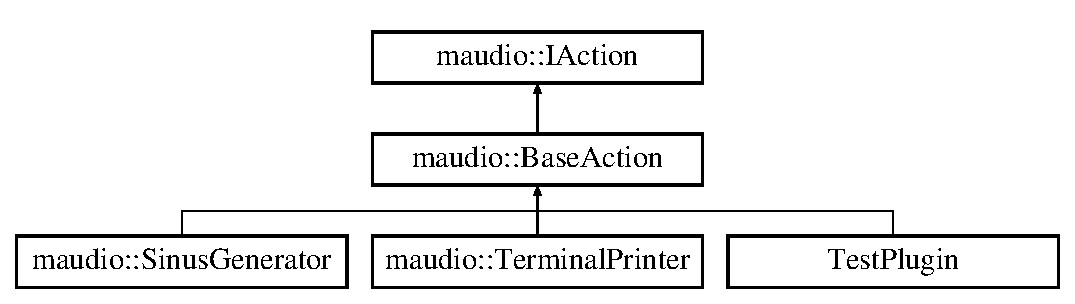
\includegraphics[height=3.000000cm]{classmaudio_1_1IAction}
\end{center}
\end{figure}
\subsection*{Public Member Functions}
\begin{DoxyCompactItemize}
\item 
virtual \hyperlink{classmaudio_1_1IAction_af416e7ca1070c5b5b48e223664831056}{$\sim$\-I\-Action} ()
\item 
virtual \hyperlink{classmaudio_1_1IAudioBuffer}{I\-Audio\-Buffer} $\ast$ \hyperlink{classmaudio_1_1IAction_adcd159456456b1104af6d4f31336fe59}{get} (unsigned long pos, unsigned int length) noexcept=0
\item 
virtual \hyperlink{classmaudio_1_1IAudioInfo}{I\-Audio\-Info} $\ast$ \hyperlink{classmaudio_1_1IAction_abf9d7d1a4d66fd1b48d946d672bfe7a0}{get\-Info} () noexcept=0
\item 
virtual void \hyperlink{classmaudio_1_1IAction_a6be8c626cd3043c4114d9cf998fd0388}{delete\-Buffer} (\hyperlink{classmaudio_1_1IAudioBuffer}{I\-Audio\-Buffer} $\ast$data) noexcept=0
\item 
virtual void \hyperlink{classmaudio_1_1IAction_af02a219faa2361dd14759e1e92003d33}{delete\-Info} (\hyperlink{classmaudio_1_1IAudioInfo}{I\-Audio\-Info} $\ast$data) noexcept=0
\item 
virtual void \hyperlink{classmaudio_1_1IAction_ae4bdc7487e1229ded107ff8d42275bd3}{delete\-Sample} (\hyperlink{classmaudio_1_1ISample}{I\-Sample} $\ast$data) noexcept=0
\item 
virtual void \hyperlink{classmaudio_1_1IAction_a0dac443df118fafeb020d2254d3c8c8a}{add\-Socket} (\hyperlink{classmaudio_1_1ISocket}{I\-Socket} $\ast$socket, int slot)=0
\item 
virtual void \hyperlink{classmaudio_1_1IAction_aa562ad351f4923aeef7d8a7c0450d74e}{remove\-Socket} (int slot)=0
\item 
virtual int \hyperlink{classmaudio_1_1IAction_ad850f2f577a12e41c71994479773079f}{Num\-Inputs} () const =0
\item 
virtual int \hyperlink{classmaudio_1_1IAction_a3c8825e7f38e0de769af7d81ccf6cf5e}{Max\-Inputs} () const =0
\item 
virtual bool \hyperlink{classmaudio_1_1IAction_a148ec76547dc1ac21e47b4b5d10c152a}{Has\-Outputs} () const =0
\item 
virtual void \hyperlink{classmaudio_1_1IAction_a610804d37c46509f3eaa1aebceab7e35}{read\-Config} (const \hyperlink{classmaudio_1_1IKeyValueStore}{I\-Key\-Value\-Store} \&conf)=0
\item 
virtual \hyperlink{classmaudio_1_1IPropertyManager}{I\-Property\-Manager} $\ast$ \hyperlink{classmaudio_1_1IAction_a59edeb0de77724d42bc51e9b7f7b6d41}{get\-Properties} ()=0
\item 
virtual \hyperlink{classmaudio_1_1IControl}{I\-Control} $\ast$ \hyperlink{classmaudio_1_1IAction_a0103686135171d24dc7901a81ae77ace}{get\-Control} ()=0
\end{DoxyCompactItemize}


\subsection{Constructor \& Destructor Documentation}
\hypertarget{classmaudio_1_1IAction_af416e7ca1070c5b5b48e223664831056}{\index{maudio\-::\-I\-Action@{maudio\-::\-I\-Action}!$\sim$\-I\-Action@{$\sim$\-I\-Action}}
\index{$\sim$\-I\-Action@{$\sim$\-I\-Action}!maudio::IAction@{maudio\-::\-I\-Action}}
\subsubsection[{$\sim$\-I\-Action}]{\setlength{\rightskip}{0pt plus 5cm}virtual maudio\-::\-I\-Action\-::$\sim$\-I\-Action (
\begin{DoxyParamCaption}
{}
\end{DoxyParamCaption}
)\hspace{0.3cm}{\ttfamily [inline]}, {\ttfamily [virtual]}}}\label{classmaudio_1_1IAction_af416e7ca1070c5b5b48e223664831056}


\subsection{Member Function Documentation}
\hypertarget{classmaudio_1_1IAction_a0dac443df118fafeb020d2254d3c8c8a}{\index{maudio\-::\-I\-Action@{maudio\-::\-I\-Action}!add\-Socket@{add\-Socket}}
\index{add\-Socket@{add\-Socket}!maudio::IAction@{maudio\-::\-I\-Action}}
\subsubsection[{add\-Socket}]{\setlength{\rightskip}{0pt plus 5cm}virtual void maudio\-::\-I\-Action\-::add\-Socket (
\begin{DoxyParamCaption}
\item[{{\bf I\-Socket} $\ast$}]{socket, }
\item[{int}]{slot}
\end{DoxyParamCaption}
)\hspace{0.3cm}{\ttfamily [pure virtual]}}}\label{classmaudio_1_1IAction_a0dac443df118fafeb020d2254d3c8c8a}


Implemented in \hyperlink{classmaudio_1_1BaseAction_a0e3fe3ae02cdf315fd63944d46419e6e}{maudio\-::\-Base\-Action}.

\hypertarget{classmaudio_1_1IAction_a6be8c626cd3043c4114d9cf998fd0388}{\index{maudio\-::\-I\-Action@{maudio\-::\-I\-Action}!delete\-Buffer@{delete\-Buffer}}
\index{delete\-Buffer@{delete\-Buffer}!maudio::IAction@{maudio\-::\-I\-Action}}
\subsubsection[{delete\-Buffer}]{\setlength{\rightskip}{0pt plus 5cm}virtual void maudio\-::\-I\-Action\-::delete\-Buffer (
\begin{DoxyParamCaption}
\item[{{\bf I\-Audio\-Buffer} $\ast$}]{data}
\end{DoxyParamCaption}
)\hspace{0.3cm}{\ttfamily [pure virtual]}, {\ttfamily [noexcept]}}}\label{classmaudio_1_1IAction_a6be8c626cd3043c4114d9cf998fd0388}


Implemented in \hyperlink{classmaudio_1_1BaseAction_a2c5422376581a5d01873833516858753}{maudio\-::\-Base\-Action}.

\hypertarget{classmaudio_1_1IAction_af02a219faa2361dd14759e1e92003d33}{\index{maudio\-::\-I\-Action@{maudio\-::\-I\-Action}!delete\-Info@{delete\-Info}}
\index{delete\-Info@{delete\-Info}!maudio::IAction@{maudio\-::\-I\-Action}}
\subsubsection[{delete\-Info}]{\setlength{\rightskip}{0pt plus 5cm}virtual void maudio\-::\-I\-Action\-::delete\-Info (
\begin{DoxyParamCaption}
\item[{{\bf I\-Audio\-Info} $\ast$}]{data}
\end{DoxyParamCaption}
)\hspace{0.3cm}{\ttfamily [pure virtual]}, {\ttfamily [noexcept]}}}\label{classmaudio_1_1IAction_af02a219faa2361dd14759e1e92003d33}


Implemented in \hyperlink{classmaudio_1_1BaseAction_ade1df46a9e5edc1931f3c061f3d51402}{maudio\-::\-Base\-Action}.

\hypertarget{classmaudio_1_1IAction_ae4bdc7487e1229ded107ff8d42275bd3}{\index{maudio\-::\-I\-Action@{maudio\-::\-I\-Action}!delete\-Sample@{delete\-Sample}}
\index{delete\-Sample@{delete\-Sample}!maudio::IAction@{maudio\-::\-I\-Action}}
\subsubsection[{delete\-Sample}]{\setlength{\rightskip}{0pt plus 5cm}virtual void maudio\-::\-I\-Action\-::delete\-Sample (
\begin{DoxyParamCaption}
\item[{{\bf I\-Sample} $\ast$}]{data}
\end{DoxyParamCaption}
)\hspace{0.3cm}{\ttfamily [pure virtual]}, {\ttfamily [noexcept]}}}\label{classmaudio_1_1IAction_ae4bdc7487e1229ded107ff8d42275bd3}


Implemented in \hyperlink{classmaudio_1_1BaseAction_a4c1f3d0c024bbdff115ac261bbf1a32c}{maudio\-::\-Base\-Action}.

\hypertarget{classmaudio_1_1IAction_adcd159456456b1104af6d4f31336fe59}{\index{maudio\-::\-I\-Action@{maudio\-::\-I\-Action}!get@{get}}
\index{get@{get}!maudio::IAction@{maudio\-::\-I\-Action}}
\subsubsection[{get}]{\setlength{\rightskip}{0pt plus 5cm}virtual {\bf I\-Audio\-Buffer}$\ast$ maudio\-::\-I\-Action\-::get (
\begin{DoxyParamCaption}
\item[{unsigned long}]{pos, }
\item[{unsigned int}]{length}
\end{DoxyParamCaption}
)\hspace{0.3cm}{\ttfamily [pure virtual]}, {\ttfamily [noexcept]}}}\label{classmaudio_1_1IAction_adcd159456456b1104af6d4f31336fe59}


Implemented in \hyperlink{classmaudio_1_1SinusGenerator_a461fdc87ced846928ea651173122713a}{maudio\-::\-Sinus\-Generator}, \hyperlink{classmaudio_1_1TerminalPrinter_a27f779bcd81b68ffad732a6da669f8fe}{maudio\-::\-Terminal\-Printer}, and \hyperlink{classTestPlugin_af45a5a7d4f61db9503d96ecc1c590251}{Test\-Plugin}.

\hypertarget{classmaudio_1_1IAction_a0103686135171d24dc7901a81ae77ace}{\index{maudio\-::\-I\-Action@{maudio\-::\-I\-Action}!get\-Control@{get\-Control}}
\index{get\-Control@{get\-Control}!maudio::IAction@{maudio\-::\-I\-Action}}
\subsubsection[{get\-Control}]{\setlength{\rightskip}{0pt plus 5cm}virtual {\bf I\-Control}$\ast$ maudio\-::\-I\-Action\-::get\-Control (
\begin{DoxyParamCaption}
{}
\end{DoxyParamCaption}
)\hspace{0.3cm}{\ttfamily [pure virtual]}}}\label{classmaudio_1_1IAction_a0103686135171d24dc7901a81ae77ace}


Implemented in \hyperlink{classmaudio_1_1BaseAction_a0ecc4f8e47f52d90b0ba7fe2757efe2c}{maudio\-::\-Base\-Action}, and \hyperlink{classmaudio_1_1TerminalPrinter_acef99a9118ebb6908166d8e97e7bb3e9}{maudio\-::\-Terminal\-Printer}.

\hypertarget{classmaudio_1_1IAction_abf9d7d1a4d66fd1b48d946d672bfe7a0}{\index{maudio\-::\-I\-Action@{maudio\-::\-I\-Action}!get\-Info@{get\-Info}}
\index{get\-Info@{get\-Info}!maudio::IAction@{maudio\-::\-I\-Action}}
\subsubsection[{get\-Info}]{\setlength{\rightskip}{0pt plus 5cm}virtual {\bf I\-Audio\-Info}$\ast$ maudio\-::\-I\-Action\-::get\-Info (
\begin{DoxyParamCaption}
{}
\end{DoxyParamCaption}
)\hspace{0.3cm}{\ttfamily [pure virtual]}, {\ttfamily [noexcept]}}}\label{classmaudio_1_1IAction_abf9d7d1a4d66fd1b48d946d672bfe7a0}


Implemented in \hyperlink{classmaudio_1_1SinusGenerator_ab3ac1d0f6d84658262026bbebcbd808f}{maudio\-::\-Sinus\-Generator}, \hyperlink{classmaudio_1_1TerminalPrinter_ae0d8b73356c360bfdd10d32ec829af85}{maudio\-::\-Terminal\-Printer}, and \hyperlink{classTestPlugin_a07aa6acf3be682c3552c88282a97ceaa}{Test\-Plugin}.

\hypertarget{classmaudio_1_1IAction_a59edeb0de77724d42bc51e9b7f7b6d41}{\index{maudio\-::\-I\-Action@{maudio\-::\-I\-Action}!get\-Properties@{get\-Properties}}
\index{get\-Properties@{get\-Properties}!maudio::IAction@{maudio\-::\-I\-Action}}
\subsubsection[{get\-Properties}]{\setlength{\rightskip}{0pt plus 5cm}virtual {\bf I\-Property\-Manager}$\ast$ maudio\-::\-I\-Action\-::get\-Properties (
\begin{DoxyParamCaption}
{}
\end{DoxyParamCaption}
)\hspace{0.3cm}{\ttfamily [pure virtual]}}}\label{classmaudio_1_1IAction_a59edeb0de77724d42bc51e9b7f7b6d41}


Implemented in \hyperlink{classmaudio_1_1BaseAction_ada21aa4734308191a32a9a2fe1dd4e3d}{maudio\-::\-Base\-Action}.

\hypertarget{classmaudio_1_1IAction_a148ec76547dc1ac21e47b4b5d10c152a}{\index{maudio\-::\-I\-Action@{maudio\-::\-I\-Action}!Has\-Outputs@{Has\-Outputs}}
\index{Has\-Outputs@{Has\-Outputs}!maudio::IAction@{maudio\-::\-I\-Action}}
\subsubsection[{Has\-Outputs}]{\setlength{\rightskip}{0pt plus 5cm}virtual bool maudio\-::\-I\-Action\-::\-Has\-Outputs (
\begin{DoxyParamCaption}
{}
\end{DoxyParamCaption}
) const\hspace{0.3cm}{\ttfamily [pure virtual]}}}\label{classmaudio_1_1IAction_a148ec76547dc1ac21e47b4b5d10c152a}


Implemented in \hyperlink{classTestPlugin_a2eb2cacb18c097fe26cc1a7640eebac3}{Test\-Plugin}, \hyperlink{classmaudio_1_1SinusGenerator_a0e39f15f11221f97fb034a42df608889}{maudio\-::\-Sinus\-Generator}, and \hyperlink{classmaudio_1_1TerminalPrinter_a3fdb9711d0d767e9acd0d01b3c7644da}{maudio\-::\-Terminal\-Printer}.

\hypertarget{classmaudio_1_1IAction_a3c8825e7f38e0de769af7d81ccf6cf5e}{\index{maudio\-::\-I\-Action@{maudio\-::\-I\-Action}!Max\-Inputs@{Max\-Inputs}}
\index{Max\-Inputs@{Max\-Inputs}!maudio::IAction@{maudio\-::\-I\-Action}}
\subsubsection[{Max\-Inputs}]{\setlength{\rightskip}{0pt plus 5cm}virtual int maudio\-::\-I\-Action\-::\-Max\-Inputs (
\begin{DoxyParamCaption}
{}
\end{DoxyParamCaption}
) const\hspace{0.3cm}{\ttfamily [pure virtual]}}}\label{classmaudio_1_1IAction_a3c8825e7f38e0de769af7d81ccf6cf5e}


Implemented in \hyperlink{classmaudio_1_1SinusGenerator_aee038f2dd2415a96ce1902be978f4ad4}{maudio\-::\-Sinus\-Generator}, \hyperlink{classTestPlugin_ad4faa8dad53c62e372e5837d8aa59ecb}{Test\-Plugin}, and \hyperlink{classmaudio_1_1TerminalPrinter_af895f464f3d51be9d44750e96dabf8f1}{maudio\-::\-Terminal\-Printer}.

\hypertarget{classmaudio_1_1IAction_ad850f2f577a12e41c71994479773079f}{\index{maudio\-::\-I\-Action@{maudio\-::\-I\-Action}!Num\-Inputs@{Num\-Inputs}}
\index{Num\-Inputs@{Num\-Inputs}!maudio::IAction@{maudio\-::\-I\-Action}}
\subsubsection[{Num\-Inputs}]{\setlength{\rightskip}{0pt plus 5cm}virtual int maudio\-::\-I\-Action\-::\-Num\-Inputs (
\begin{DoxyParamCaption}
{}
\end{DoxyParamCaption}
) const\hspace{0.3cm}{\ttfamily [pure virtual]}}}\label{classmaudio_1_1IAction_ad850f2f577a12e41c71994479773079f}


Implemented in \hyperlink{classmaudio_1_1BaseAction_a25f6c6801b1643bdc0a2bc9bb3534654}{maudio\-::\-Base\-Action}.

\hypertarget{classmaudio_1_1IAction_a610804d37c46509f3eaa1aebceab7e35}{\index{maudio\-::\-I\-Action@{maudio\-::\-I\-Action}!read\-Config@{read\-Config}}
\index{read\-Config@{read\-Config}!maudio::IAction@{maudio\-::\-I\-Action}}
\subsubsection[{read\-Config}]{\setlength{\rightskip}{0pt plus 5cm}virtual void maudio\-::\-I\-Action\-::read\-Config (
\begin{DoxyParamCaption}
\item[{const {\bf I\-Key\-Value\-Store} \&}]{conf}
\end{DoxyParamCaption}
)\hspace{0.3cm}{\ttfamily [pure virtual]}}}\label{classmaudio_1_1IAction_a610804d37c46509f3eaa1aebceab7e35}


Implemented in \hyperlink{classTestPlugin_acd8d80abecd3967547e401cba0e1b660}{Test\-Plugin}, \hyperlink{classmaudio_1_1SinusGenerator_a9a901592dba8df35ac74ddd85cbb1482}{maudio\-::\-Sinus\-Generator}, and \hyperlink{classmaudio_1_1TerminalPrinter_a3888206cd622627b441ca00cca6d87e2}{maudio\-::\-Terminal\-Printer}.

\hypertarget{classmaudio_1_1IAction_aa562ad351f4923aeef7d8a7c0450d74e}{\index{maudio\-::\-I\-Action@{maudio\-::\-I\-Action}!remove\-Socket@{remove\-Socket}}
\index{remove\-Socket@{remove\-Socket}!maudio::IAction@{maudio\-::\-I\-Action}}
\subsubsection[{remove\-Socket}]{\setlength{\rightskip}{0pt plus 5cm}virtual void maudio\-::\-I\-Action\-::remove\-Socket (
\begin{DoxyParamCaption}
\item[{int}]{slot}
\end{DoxyParamCaption}
)\hspace{0.3cm}{\ttfamily [pure virtual]}}}\label{classmaudio_1_1IAction_aa562ad351f4923aeef7d8a7c0450d74e}


Implemented in \hyperlink{classmaudio_1_1BaseAction_aac97bab055f68c49941dbaae9a1ff497}{maudio\-::\-Base\-Action}.



The documentation for this class was generated from the following file\-:\begin{DoxyCompactItemize}
\item 
/home/mars/\-Projekte/maudio/src/plugins/include/core/node/\hyperlink{IAction_8hpp}{I\-Action.\-hpp}\end{DoxyCompactItemize}

\hypertarget{classmaudio_1_1IAudioBuffer}{\section{maudio\-:\-:I\-Audio\-Buffer Class Reference}
\label{classmaudio_1_1IAudioBuffer}\index{maudio\-::\-I\-Audio\-Buffer@{maudio\-::\-I\-Audio\-Buffer}}
}


holds an audio stream in a vector of floats  




{\ttfamily \#include $<$I\-Audio\-Buffer.\-hpp$>$}

Inheritance diagram for maudio\-:\-:I\-Audio\-Buffer\-:\begin{figure}[H]
\begin{center}
\leavevmode
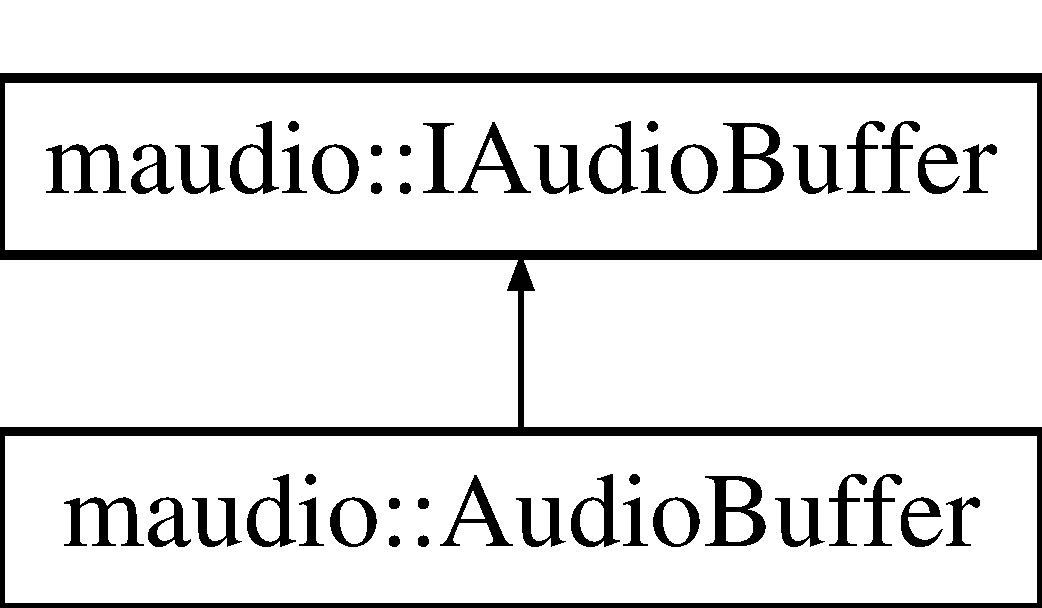
\includegraphics[height=2.000000cm]{classmaudio_1_1IAudioBuffer}
\end{center}
\end{figure}
\subsection*{Public Member Functions}
\begin{DoxyCompactItemize}
\item 
virtual \hyperlink{classmaudio_1_1IAudioBuffer_aaec85fcb95eec6f7cf3913300131015c}{$\sim$\-I\-Audio\-Buffer} ()
\item 
virtual \hyperlink{classmaudio_1_1ISample}{I\-Sample} $\ast$ \hyperlink{classmaudio_1_1IAudioBuffer_a32a5742929553887a22e4d48be0e3763}{operator\mbox{[}$\,$\mbox{]}} (unsigned long pos) const =0
\item 
virtual \hyperlink{classmaudio_1_1ISample}{I\-Sample} $\ast$ \hyperlink{classmaudio_1_1IAudioBuffer_aaea60a9702071ae0b12e9e616e72defb}{get} (unsigned long pos) const =0
\item 
virtual void \hyperlink{classmaudio_1_1IAudioBuffer_ab8f8728745907781bc31508d5816ef60}{set} (const \hyperlink{classmaudio_1_1ISample}{I\-Sample} \&data, unsigned long pos)=0
\item 
virtual void \hyperlink{classmaudio_1_1IAudioBuffer_a50d44964ef18c7dfd483fd0e68294d6b}{resize} (unsigned long samples)=0
\item 
virtual const \hyperlink{classmaudio_1_1IAudioInfo}{I\-Audio\-Info} $\ast$ \hyperlink{classmaudio_1_1IAudioBuffer_afd0eb3d169bade19e4508a4eaa2a07b4}{get\-Info} () const =0
\item 
virtual const float $\ast$ \hyperlink{classmaudio_1_1IAudioBuffer_a60f486dc3d94b4c4f06df698e7848117}{get\-Raw} () const =0
\end{DoxyCompactItemize}


\subsection{Detailed Description}
holds an audio stream in a vector of floats 

\subsection{Constructor \& Destructor Documentation}
\hypertarget{classmaudio_1_1IAudioBuffer_aaec85fcb95eec6f7cf3913300131015c}{\index{maudio\-::\-I\-Audio\-Buffer@{maudio\-::\-I\-Audio\-Buffer}!$\sim$\-I\-Audio\-Buffer@{$\sim$\-I\-Audio\-Buffer}}
\index{$\sim$\-I\-Audio\-Buffer@{$\sim$\-I\-Audio\-Buffer}!maudio::IAudioBuffer@{maudio\-::\-I\-Audio\-Buffer}}
\subsubsection[{$\sim$\-I\-Audio\-Buffer}]{\setlength{\rightskip}{0pt plus 5cm}virtual maudio\-::\-I\-Audio\-Buffer\-::$\sim$\-I\-Audio\-Buffer (
\begin{DoxyParamCaption}
{}
\end{DoxyParamCaption}
)\hspace{0.3cm}{\ttfamily [inline]}, {\ttfamily [virtual]}}}\label{classmaudio_1_1IAudioBuffer_aaec85fcb95eec6f7cf3913300131015c}


\subsection{Member Function Documentation}
\hypertarget{classmaudio_1_1IAudioBuffer_aaea60a9702071ae0b12e9e616e72defb}{\index{maudio\-::\-I\-Audio\-Buffer@{maudio\-::\-I\-Audio\-Buffer}!get@{get}}
\index{get@{get}!maudio::IAudioBuffer@{maudio\-::\-I\-Audio\-Buffer}}
\subsubsection[{get}]{\setlength{\rightskip}{0pt plus 5cm}virtual {\bf I\-Sample}$\ast$ maudio\-::\-I\-Audio\-Buffer\-::get (
\begin{DoxyParamCaption}
\item[{unsigned long}]{pos}
\end{DoxyParamCaption}
) const\hspace{0.3cm}{\ttfamily [pure virtual]}}}\label{classmaudio_1_1IAudioBuffer_aaea60a9702071ae0b12e9e616e72defb}


Implemented in \hyperlink{classmaudio_1_1AudioBuffer_a93eeb4f2f16bf113e8bc77592d7c4664}{maudio\-::\-Audio\-Buffer}.

\hypertarget{classmaudio_1_1IAudioBuffer_afd0eb3d169bade19e4508a4eaa2a07b4}{\index{maudio\-::\-I\-Audio\-Buffer@{maudio\-::\-I\-Audio\-Buffer}!get\-Info@{get\-Info}}
\index{get\-Info@{get\-Info}!maudio::IAudioBuffer@{maudio\-::\-I\-Audio\-Buffer}}
\subsubsection[{get\-Info}]{\setlength{\rightskip}{0pt plus 5cm}virtual const {\bf I\-Audio\-Info}$\ast$ maudio\-::\-I\-Audio\-Buffer\-::get\-Info (
\begin{DoxyParamCaption}
{}
\end{DoxyParamCaption}
) const\hspace{0.3cm}{\ttfamily [pure virtual]}}}\label{classmaudio_1_1IAudioBuffer_afd0eb3d169bade19e4508a4eaa2a07b4}


Implemented in \hyperlink{classmaudio_1_1AudioBuffer_aa5e0294c0de7b4bbcaed0afa9ae22728}{maudio\-::\-Audio\-Buffer}.

\hypertarget{classmaudio_1_1IAudioBuffer_a60f486dc3d94b4c4f06df698e7848117}{\index{maudio\-::\-I\-Audio\-Buffer@{maudio\-::\-I\-Audio\-Buffer}!get\-Raw@{get\-Raw}}
\index{get\-Raw@{get\-Raw}!maudio::IAudioBuffer@{maudio\-::\-I\-Audio\-Buffer}}
\subsubsection[{get\-Raw}]{\setlength{\rightskip}{0pt plus 5cm}virtual const float$\ast$ maudio\-::\-I\-Audio\-Buffer\-::get\-Raw (
\begin{DoxyParamCaption}
{}
\end{DoxyParamCaption}
) const\hspace{0.3cm}{\ttfamily [pure virtual]}}}\label{classmaudio_1_1IAudioBuffer_a60f486dc3d94b4c4f06df698e7848117}


Implemented in \hyperlink{classmaudio_1_1AudioBuffer_a6ac54537437e8a3fc4236b9375dc0126}{maudio\-::\-Audio\-Buffer}.

\hypertarget{classmaudio_1_1IAudioBuffer_a32a5742929553887a22e4d48be0e3763}{\index{maudio\-::\-I\-Audio\-Buffer@{maudio\-::\-I\-Audio\-Buffer}!operator\mbox{[}$\,$\mbox{]}@{operator[]}}
\index{operator\mbox{[}$\,$\mbox{]}@{operator[]}!maudio::IAudioBuffer@{maudio\-::\-I\-Audio\-Buffer}}
\subsubsection[{operator[]}]{\setlength{\rightskip}{0pt plus 5cm}virtual {\bf I\-Sample}$\ast$ maudio\-::\-I\-Audio\-Buffer\-::operator\mbox{[}$\,$\mbox{]} (
\begin{DoxyParamCaption}
\item[{unsigned long}]{pos}
\end{DoxyParamCaption}
) const\hspace{0.3cm}{\ttfamily [pure virtual]}}}\label{classmaudio_1_1IAudioBuffer_a32a5742929553887a22e4d48be0e3763}


Implemented in \hyperlink{classmaudio_1_1AudioBuffer_a6548ddb981ec41fa92d821a15aa06080}{maudio\-::\-Audio\-Buffer}.

\hypertarget{classmaudio_1_1IAudioBuffer_a50d44964ef18c7dfd483fd0e68294d6b}{\index{maudio\-::\-I\-Audio\-Buffer@{maudio\-::\-I\-Audio\-Buffer}!resize@{resize}}
\index{resize@{resize}!maudio::IAudioBuffer@{maudio\-::\-I\-Audio\-Buffer}}
\subsubsection[{resize}]{\setlength{\rightskip}{0pt plus 5cm}virtual void maudio\-::\-I\-Audio\-Buffer\-::resize (
\begin{DoxyParamCaption}
\item[{unsigned long}]{samples}
\end{DoxyParamCaption}
)\hspace{0.3cm}{\ttfamily [pure virtual]}}}\label{classmaudio_1_1IAudioBuffer_a50d44964ef18c7dfd483fd0e68294d6b}


Implemented in \hyperlink{classmaudio_1_1AudioBuffer_aeed134c3a1b7f5446594fa23c8857e8c}{maudio\-::\-Audio\-Buffer}.

\hypertarget{classmaudio_1_1IAudioBuffer_ab8f8728745907781bc31508d5816ef60}{\index{maudio\-::\-I\-Audio\-Buffer@{maudio\-::\-I\-Audio\-Buffer}!set@{set}}
\index{set@{set}!maudio::IAudioBuffer@{maudio\-::\-I\-Audio\-Buffer}}
\subsubsection[{set}]{\setlength{\rightskip}{0pt plus 5cm}virtual void maudio\-::\-I\-Audio\-Buffer\-::set (
\begin{DoxyParamCaption}
\item[{const {\bf I\-Sample} \&}]{data, }
\item[{unsigned long}]{pos}
\end{DoxyParamCaption}
)\hspace{0.3cm}{\ttfamily [pure virtual]}}}\label{classmaudio_1_1IAudioBuffer_ab8f8728745907781bc31508d5816ef60}


Implemented in \hyperlink{classmaudio_1_1AudioBuffer_a3f19c9611c89947bbf27af7f788b8347}{maudio\-::\-Audio\-Buffer}.



The documentation for this class was generated from the following file\-:\begin{DoxyCompactItemize}
\item 
/home/mars/\-Projekte/maudio/src/plugins/include/core/audiodata/\hyperlink{IAudioBuffer_8hpp}{I\-Audio\-Buffer.\-hpp}\end{DoxyCompactItemize}

\hypertarget{classmaudio_1_1IAudioInfo}{\section{maudio\-:\-:I\-Audio\-Info Class Reference}
\label{classmaudio_1_1IAudioInfo}\index{maudio\-::\-I\-Audio\-Info@{maudio\-::\-I\-Audio\-Info}}
}


{\ttfamily \#include $<$I\-Audio\-Info.\-hpp$>$}

Inheritance diagram for maudio\-:\-:I\-Audio\-Info\-:\begin{figure}[H]
\begin{center}
\leavevmode
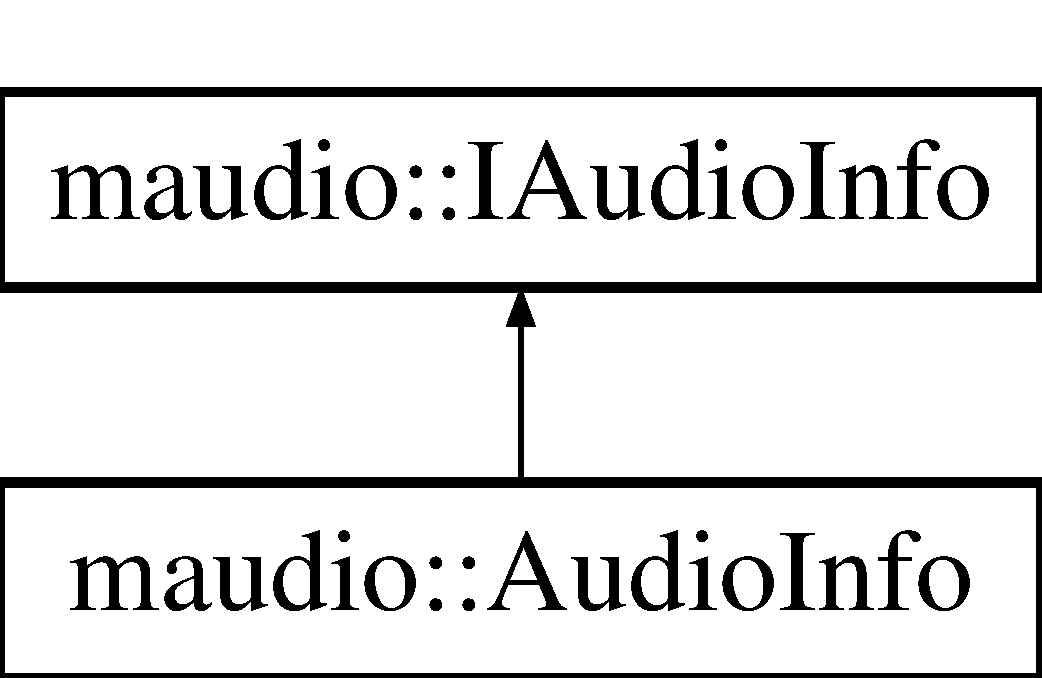
\includegraphics[height=2.000000cm]{classmaudio_1_1IAudioInfo}
\end{center}
\end{figure}
\subsection*{Public Member Functions}
\begin{DoxyCompactItemize}
\item 
virtual \hyperlink{classmaudio_1_1IAudioInfo_aff8c17f3657c997ee2ea0aadf31e989c}{$\sim$\-I\-Audio\-Info} ()
\item 
virtual unsigned long \hyperlink{classmaudio_1_1IAudioInfo_a88a698d7169f5c21118b83b8afcd1bf6}{get\-Samples} () const =0
\item 
virtual unsigned long \hyperlink{classmaudio_1_1IAudioInfo_ab85da546b049d23c400c8a869ea1e103}{get\-Offset} () const =0
\item 
virtual unsigned int \hyperlink{classmaudio_1_1IAudioInfo_a557f464eb6a2feb2ce24dfae5a85d727}{get\-Samplerate} () const =0
\item 
virtual unsigned int \hyperlink{classmaudio_1_1IAudioInfo_a5b412da4d44d7939b4927ec932c74a83}{get\-Channels} () const =0
\item 
virtual void \hyperlink{classmaudio_1_1IAudioInfo_ab2b4c49c21fa711f457650cc377271bb}{set\-Samples} (unsigned long samples)=0
\item 
virtual void \hyperlink{classmaudio_1_1IAudioInfo_a333fc60d8bf76b82bc0a65b8c6a77e4f}{set\-Offset} (unsigned long offset)=0
\item 
virtual void \hyperlink{classmaudio_1_1IAudioInfo_a2a54df3fc726ccb2b0994bc8e3d15c37}{set\-Samplerate} (unsigned int samplerate)=0
\item 
virtual void \hyperlink{classmaudio_1_1IAudioInfo_aaae3741d16b6c0dc531084876940a0f4}{set\-Channels} (unsigned int channels)=0
\end{DoxyCompactItemize}


\subsection{Constructor \& Destructor Documentation}
\hypertarget{classmaudio_1_1IAudioInfo_aff8c17f3657c997ee2ea0aadf31e989c}{\index{maudio\-::\-I\-Audio\-Info@{maudio\-::\-I\-Audio\-Info}!$\sim$\-I\-Audio\-Info@{$\sim$\-I\-Audio\-Info}}
\index{$\sim$\-I\-Audio\-Info@{$\sim$\-I\-Audio\-Info}!maudio::IAudioInfo@{maudio\-::\-I\-Audio\-Info}}
\subsubsection[{$\sim$\-I\-Audio\-Info}]{\setlength{\rightskip}{0pt plus 5cm}virtual maudio\-::\-I\-Audio\-Info\-::$\sim$\-I\-Audio\-Info (
\begin{DoxyParamCaption}
{}
\end{DoxyParamCaption}
)\hspace{0.3cm}{\ttfamily [inline]}, {\ttfamily [virtual]}}}\label{classmaudio_1_1IAudioInfo_aff8c17f3657c997ee2ea0aadf31e989c}


\subsection{Member Function Documentation}
\hypertarget{classmaudio_1_1IAudioInfo_a5b412da4d44d7939b4927ec932c74a83}{\index{maudio\-::\-I\-Audio\-Info@{maudio\-::\-I\-Audio\-Info}!get\-Channels@{get\-Channels}}
\index{get\-Channels@{get\-Channels}!maudio::IAudioInfo@{maudio\-::\-I\-Audio\-Info}}
\subsubsection[{get\-Channels}]{\setlength{\rightskip}{0pt plus 5cm}virtual unsigned int maudio\-::\-I\-Audio\-Info\-::get\-Channels (
\begin{DoxyParamCaption}
{}
\end{DoxyParamCaption}
) const\hspace{0.3cm}{\ttfamily [pure virtual]}}}\label{classmaudio_1_1IAudioInfo_a5b412da4d44d7939b4927ec932c74a83}


Implemented in \hyperlink{classmaudio_1_1AudioInfo_af4d1f9d433e4d29e218ec28bee4ed7db}{maudio\-::\-Audio\-Info}.

\hypertarget{classmaudio_1_1IAudioInfo_ab85da546b049d23c400c8a869ea1e103}{\index{maudio\-::\-I\-Audio\-Info@{maudio\-::\-I\-Audio\-Info}!get\-Offset@{get\-Offset}}
\index{get\-Offset@{get\-Offset}!maudio::IAudioInfo@{maudio\-::\-I\-Audio\-Info}}
\subsubsection[{get\-Offset}]{\setlength{\rightskip}{0pt plus 5cm}virtual unsigned long maudio\-::\-I\-Audio\-Info\-::get\-Offset (
\begin{DoxyParamCaption}
{}
\end{DoxyParamCaption}
) const\hspace{0.3cm}{\ttfamily [pure virtual]}}}\label{classmaudio_1_1IAudioInfo_ab85da546b049d23c400c8a869ea1e103}


Implemented in \hyperlink{classmaudio_1_1AudioInfo_ad89ed92138ad9e3e5b098bee69a9bd96}{maudio\-::\-Audio\-Info}.

\hypertarget{classmaudio_1_1IAudioInfo_a557f464eb6a2feb2ce24dfae5a85d727}{\index{maudio\-::\-I\-Audio\-Info@{maudio\-::\-I\-Audio\-Info}!get\-Samplerate@{get\-Samplerate}}
\index{get\-Samplerate@{get\-Samplerate}!maudio::IAudioInfo@{maudio\-::\-I\-Audio\-Info}}
\subsubsection[{get\-Samplerate}]{\setlength{\rightskip}{0pt plus 5cm}virtual unsigned int maudio\-::\-I\-Audio\-Info\-::get\-Samplerate (
\begin{DoxyParamCaption}
{}
\end{DoxyParamCaption}
) const\hspace{0.3cm}{\ttfamily [pure virtual]}}}\label{classmaudio_1_1IAudioInfo_a557f464eb6a2feb2ce24dfae5a85d727}


Implemented in \hyperlink{classmaudio_1_1AudioInfo_a92e76f5173ea34dfdd0ca42ff0662a6f}{maudio\-::\-Audio\-Info}.

\hypertarget{classmaudio_1_1IAudioInfo_a88a698d7169f5c21118b83b8afcd1bf6}{\index{maudio\-::\-I\-Audio\-Info@{maudio\-::\-I\-Audio\-Info}!get\-Samples@{get\-Samples}}
\index{get\-Samples@{get\-Samples}!maudio::IAudioInfo@{maudio\-::\-I\-Audio\-Info}}
\subsubsection[{get\-Samples}]{\setlength{\rightskip}{0pt plus 5cm}virtual unsigned long maudio\-::\-I\-Audio\-Info\-::get\-Samples (
\begin{DoxyParamCaption}
{}
\end{DoxyParamCaption}
) const\hspace{0.3cm}{\ttfamily [pure virtual]}}}\label{classmaudio_1_1IAudioInfo_a88a698d7169f5c21118b83b8afcd1bf6}


Implemented in \hyperlink{classmaudio_1_1AudioInfo_aefb17a9c4301d9dcf6e5c04597892dbd}{maudio\-::\-Audio\-Info}.

\hypertarget{classmaudio_1_1IAudioInfo_aaae3741d16b6c0dc531084876940a0f4}{\index{maudio\-::\-I\-Audio\-Info@{maudio\-::\-I\-Audio\-Info}!set\-Channels@{set\-Channels}}
\index{set\-Channels@{set\-Channels}!maudio::IAudioInfo@{maudio\-::\-I\-Audio\-Info}}
\subsubsection[{set\-Channels}]{\setlength{\rightskip}{0pt plus 5cm}virtual void maudio\-::\-I\-Audio\-Info\-::set\-Channels (
\begin{DoxyParamCaption}
\item[{unsigned int}]{channels}
\end{DoxyParamCaption}
)\hspace{0.3cm}{\ttfamily [pure virtual]}}}\label{classmaudio_1_1IAudioInfo_aaae3741d16b6c0dc531084876940a0f4}


Implemented in \hyperlink{classmaudio_1_1AudioInfo_addb04eb7024304a625ef9304fa03dee9}{maudio\-::\-Audio\-Info}.

\hypertarget{classmaudio_1_1IAudioInfo_a333fc60d8bf76b82bc0a65b8c6a77e4f}{\index{maudio\-::\-I\-Audio\-Info@{maudio\-::\-I\-Audio\-Info}!set\-Offset@{set\-Offset}}
\index{set\-Offset@{set\-Offset}!maudio::IAudioInfo@{maudio\-::\-I\-Audio\-Info}}
\subsubsection[{set\-Offset}]{\setlength{\rightskip}{0pt plus 5cm}virtual void maudio\-::\-I\-Audio\-Info\-::set\-Offset (
\begin{DoxyParamCaption}
\item[{unsigned long}]{offset}
\end{DoxyParamCaption}
)\hspace{0.3cm}{\ttfamily [pure virtual]}}}\label{classmaudio_1_1IAudioInfo_a333fc60d8bf76b82bc0a65b8c6a77e4f}


Implemented in \hyperlink{classmaudio_1_1AudioInfo_aa1db33ccc763532a5d2858c00b65303a}{maudio\-::\-Audio\-Info}.

\hypertarget{classmaudio_1_1IAudioInfo_a2a54df3fc726ccb2b0994bc8e3d15c37}{\index{maudio\-::\-I\-Audio\-Info@{maudio\-::\-I\-Audio\-Info}!set\-Samplerate@{set\-Samplerate}}
\index{set\-Samplerate@{set\-Samplerate}!maudio::IAudioInfo@{maudio\-::\-I\-Audio\-Info}}
\subsubsection[{set\-Samplerate}]{\setlength{\rightskip}{0pt plus 5cm}virtual void maudio\-::\-I\-Audio\-Info\-::set\-Samplerate (
\begin{DoxyParamCaption}
\item[{unsigned int}]{samplerate}
\end{DoxyParamCaption}
)\hspace{0.3cm}{\ttfamily [pure virtual]}}}\label{classmaudio_1_1IAudioInfo_a2a54df3fc726ccb2b0994bc8e3d15c37}


Implemented in \hyperlink{classmaudio_1_1AudioInfo_a5c466cc04ed7611522ad9ab626b101f5}{maudio\-::\-Audio\-Info}.

\hypertarget{classmaudio_1_1IAudioInfo_ab2b4c49c21fa711f457650cc377271bb}{\index{maudio\-::\-I\-Audio\-Info@{maudio\-::\-I\-Audio\-Info}!set\-Samples@{set\-Samples}}
\index{set\-Samples@{set\-Samples}!maudio::IAudioInfo@{maudio\-::\-I\-Audio\-Info}}
\subsubsection[{set\-Samples}]{\setlength{\rightskip}{0pt plus 5cm}virtual void maudio\-::\-I\-Audio\-Info\-::set\-Samples (
\begin{DoxyParamCaption}
\item[{unsigned long}]{samples}
\end{DoxyParamCaption}
)\hspace{0.3cm}{\ttfamily [pure virtual]}}}\label{classmaudio_1_1IAudioInfo_ab2b4c49c21fa711f457650cc377271bb}


Implemented in \hyperlink{classmaudio_1_1AudioInfo_aa75d37ecf53cca3a0b7cecfb004da207}{maudio\-::\-Audio\-Info}.



The documentation for this class was generated from the following file\-:\begin{DoxyCompactItemize}
\item 
/home/mars/\-Projekte/maudio/src/plugins/include/core/audiodata/\hyperlink{IAudioInfo_8hpp}{I\-Audio\-Info.\-hpp}\end{DoxyCompactItemize}

\hypertarget{classmaudio_1_1IControl}{\section{maudio\-:\-:I\-Control Class Reference}
\label{classmaudio_1_1IControl}\index{maudio\-::\-I\-Control@{maudio\-::\-I\-Control}}
}


{\ttfamily \#include $<$I\-Control.\-hpp$>$}

\subsection*{Public Member Functions}
\begin{DoxyCompactItemize}
\item 
virtual \hyperlink{classmaudio_1_1IControl_ad444d545e16d3d73ab06c84b902f9741}{$\sim$\-I\-Control} ()
\item 
virtual unsigned int \hyperlink{classmaudio_1_1IControl_ab04238265cb6854c570a1e982c2c1fe0}{get\-Num\-Functions} ()=0
\item 
virtual const char $\ast$ \hyperlink{classmaudio_1_1IControl_a1961f5171b294b4eceddb4380f9e75ab}{get\-Function\-Name} (unsigned int num)=0
\item 
virtual const char $\ast$ \hyperlink{classmaudio_1_1IControl_a4ed7fa3a3838496027ba54f2b0e9bf03}{get\-Function\-Param} (unsigned int num)=0
\item 
virtual unsigned int \hyperlink{classmaudio_1_1IControl_ad590d52c672460533758d7b4686e807f}{call\-Function} (unsigned int num, const char $\ast$param=N\-U\-L\-L)=0
\item 
virtual unsigned int \hyperlink{classmaudio_1_1IControl_a91a034cdc9edfb80e6213a447541b726}{call\-Function} (const char $\ast$name, const char $\ast$param=N\-U\-L\-L)=0
\end{DoxyCompactItemize}


\subsection{Constructor \& Destructor Documentation}
\hypertarget{classmaudio_1_1IControl_ad444d545e16d3d73ab06c84b902f9741}{\index{maudio\-::\-I\-Control@{maudio\-::\-I\-Control}!$\sim$\-I\-Control@{$\sim$\-I\-Control}}
\index{$\sim$\-I\-Control@{$\sim$\-I\-Control}!maudio::IControl@{maudio\-::\-I\-Control}}
\subsubsection[{$\sim$\-I\-Control}]{\setlength{\rightskip}{0pt plus 5cm}virtual maudio\-::\-I\-Control\-::$\sim$\-I\-Control (
\begin{DoxyParamCaption}
{}
\end{DoxyParamCaption}
)\hspace{0.3cm}{\ttfamily [inline]}, {\ttfamily [virtual]}}}\label{classmaudio_1_1IControl_ad444d545e16d3d73ab06c84b902f9741}


\subsection{Member Function Documentation}
\hypertarget{classmaudio_1_1IControl_ad590d52c672460533758d7b4686e807f}{\index{maudio\-::\-I\-Control@{maudio\-::\-I\-Control}!call\-Function@{call\-Function}}
\index{call\-Function@{call\-Function}!maudio::IControl@{maudio\-::\-I\-Control}}
\subsubsection[{call\-Function}]{\setlength{\rightskip}{0pt plus 5cm}virtual unsigned int maudio\-::\-I\-Control\-::call\-Function (
\begin{DoxyParamCaption}
\item[{unsigned int}]{num, }
\item[{const char $\ast$}]{param = {\ttfamily NULL}}
\end{DoxyParamCaption}
)\hspace{0.3cm}{\ttfamily [pure virtual]}}}\label{classmaudio_1_1IControl_ad590d52c672460533758d7b4686e807f}
\hypertarget{classmaudio_1_1IControl_a91a034cdc9edfb80e6213a447541b726}{\index{maudio\-::\-I\-Control@{maudio\-::\-I\-Control}!call\-Function@{call\-Function}}
\index{call\-Function@{call\-Function}!maudio::IControl@{maudio\-::\-I\-Control}}
\subsubsection[{call\-Function}]{\setlength{\rightskip}{0pt plus 5cm}virtual unsigned int maudio\-::\-I\-Control\-::call\-Function (
\begin{DoxyParamCaption}
\item[{const char $\ast$}]{name, }
\item[{const char $\ast$}]{param = {\ttfamily NULL}}
\end{DoxyParamCaption}
)\hspace{0.3cm}{\ttfamily [pure virtual]}}}\label{classmaudio_1_1IControl_a91a034cdc9edfb80e6213a447541b726}
\hypertarget{classmaudio_1_1IControl_a1961f5171b294b4eceddb4380f9e75ab}{\index{maudio\-::\-I\-Control@{maudio\-::\-I\-Control}!get\-Function\-Name@{get\-Function\-Name}}
\index{get\-Function\-Name@{get\-Function\-Name}!maudio::IControl@{maudio\-::\-I\-Control}}
\subsubsection[{get\-Function\-Name}]{\setlength{\rightskip}{0pt plus 5cm}virtual const char$\ast$ maudio\-::\-I\-Control\-::get\-Function\-Name (
\begin{DoxyParamCaption}
\item[{unsigned int}]{num}
\end{DoxyParamCaption}
)\hspace{0.3cm}{\ttfamily [pure virtual]}}}\label{classmaudio_1_1IControl_a1961f5171b294b4eceddb4380f9e75ab}
\hypertarget{classmaudio_1_1IControl_a4ed7fa3a3838496027ba54f2b0e9bf03}{\index{maudio\-::\-I\-Control@{maudio\-::\-I\-Control}!get\-Function\-Param@{get\-Function\-Param}}
\index{get\-Function\-Param@{get\-Function\-Param}!maudio::IControl@{maudio\-::\-I\-Control}}
\subsubsection[{get\-Function\-Param}]{\setlength{\rightskip}{0pt plus 5cm}virtual const char$\ast$ maudio\-::\-I\-Control\-::get\-Function\-Param (
\begin{DoxyParamCaption}
\item[{unsigned int}]{num}
\end{DoxyParamCaption}
)\hspace{0.3cm}{\ttfamily [pure virtual]}}}\label{classmaudio_1_1IControl_a4ed7fa3a3838496027ba54f2b0e9bf03}
\hypertarget{classmaudio_1_1IControl_ab04238265cb6854c570a1e982c2c1fe0}{\index{maudio\-::\-I\-Control@{maudio\-::\-I\-Control}!get\-Num\-Functions@{get\-Num\-Functions}}
\index{get\-Num\-Functions@{get\-Num\-Functions}!maudio::IControl@{maudio\-::\-I\-Control}}
\subsubsection[{get\-Num\-Functions}]{\setlength{\rightskip}{0pt plus 5cm}virtual unsigned int maudio\-::\-I\-Control\-::get\-Num\-Functions (
\begin{DoxyParamCaption}
{}
\end{DoxyParamCaption}
)\hspace{0.3cm}{\ttfamily [pure virtual]}}}\label{classmaudio_1_1IControl_ab04238265cb6854c570a1e982c2c1fe0}


The documentation for this class was generated from the following file\-:\begin{DoxyCompactItemize}
\item 
/home/mars/\-Projekte/maudio/src/plugins/include/core/node/\hyperlink{IControl_8hpp}{I\-Control.\-hpp}\end{DoxyCompactItemize}

\hypertarget{classmaudio_1_1IKeyableProperty}{\section{maudio\-:\-:I\-Keyable\-Property Class Reference}
\label{classmaudio_1_1IKeyableProperty}\index{maudio\-::\-I\-Keyable\-Property@{maudio\-::\-I\-Keyable\-Property}}
}


{\ttfamily \#include $<$I\-Keyable\-Property.\-hpp$>$}

Inheritance diagram for maudio\-:\-:I\-Keyable\-Property\-:\begin{figure}[H]
\begin{center}
\leavevmode
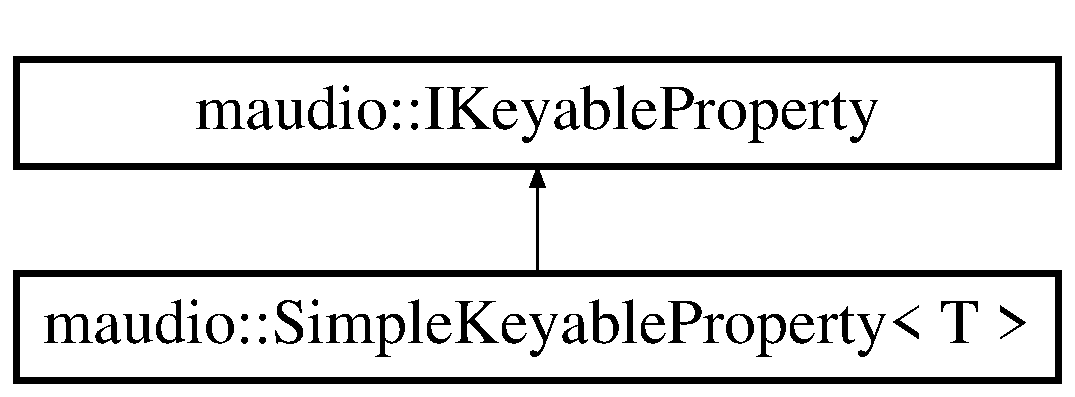
\includegraphics[height=2.000000cm]{classmaudio_1_1IKeyableProperty}
\end{center}
\end{figure}
\subsection*{Public Member Functions}
\begin{DoxyCompactItemize}
\item 
virtual \hyperlink{classmaudio_1_1IKeyableProperty_a252ca5ad4a6b92d9c7adb197b247df4b}{$\sim$\-I\-Keyable\-Property} ()
\item 
virtual const char $\ast$ \hyperlink{classmaudio_1_1IKeyableProperty_a7f216d19b9074b2bda72b54e1c3034ea}{get\-Name} () const =0
\item 
virtual const char $\ast$ \hyperlink{classmaudio_1_1IKeyableProperty_af28a9b9fb457b638624257cdfb2fbeef}{get\-String} (long double pos) const =0
\item 
virtual const char $\ast$ \hyperlink{classmaudio_1_1IKeyableProperty_a219e9bbe5f66145aeb5d7449e0598220}{get\-Key\-String} (unsigned int keynum) const =0
\item 
virtual long double \hyperlink{classmaudio_1_1IKeyableProperty_a6412f2574d0ca4948b81ba62efd695c3}{get\-Key\-Pos} (unsigned int keynum) const =0
\item 
virtual unsigned int \hyperlink{classmaudio_1_1IKeyableProperty_a471a706e69c4c42679fd2e3bd40dee5f}{get\-Num\-Keys} () const =0
\item 
virtual void \hyperlink{classmaudio_1_1IKeyableProperty_abdfffe5b0cdd27083714826014d2dfd9}{add\-Key} (const char $\ast$value, long double pos)=0
\item 
virtual void \hyperlink{classmaudio_1_1IKeyableProperty_ab2785fc6f55d610971f17573d0f5c010}{set\-Key} (const char $\ast$value, unsigned int keynum)=0
\item 
virtual void \hyperlink{classmaudio_1_1IKeyableProperty_a33844ec902186c6c051c833c9a72b33f}{remove\-Key} (unsigned int keynum)=0
\item 
virtual const char $\ast$ \hyperlink{classmaudio_1_1IKeyableProperty_aca107fbec3117a448c48c2cf4f226198}{get\-Bottom\-Bounds\-String} () const =0
\item 
virtual const char $\ast$ \hyperlink{classmaudio_1_1IKeyableProperty_a0cd30ce4a45a13e386968f9890eaada0}{get\-Upper\-Bounds\-String} () const =0
\end{DoxyCompactItemize}


\subsection{Constructor \& Destructor Documentation}
\hypertarget{classmaudio_1_1IKeyableProperty_a252ca5ad4a6b92d9c7adb197b247df4b}{\index{maudio\-::\-I\-Keyable\-Property@{maudio\-::\-I\-Keyable\-Property}!$\sim$\-I\-Keyable\-Property@{$\sim$\-I\-Keyable\-Property}}
\index{$\sim$\-I\-Keyable\-Property@{$\sim$\-I\-Keyable\-Property}!maudio::IKeyableProperty@{maudio\-::\-I\-Keyable\-Property}}
\subsubsection[{$\sim$\-I\-Keyable\-Property}]{\setlength{\rightskip}{0pt plus 5cm}virtual maudio\-::\-I\-Keyable\-Property\-::$\sim$\-I\-Keyable\-Property (
\begin{DoxyParamCaption}
{}
\end{DoxyParamCaption}
)\hspace{0.3cm}{\ttfamily [inline]}, {\ttfamily [virtual]}}}\label{classmaudio_1_1IKeyableProperty_a252ca5ad4a6b92d9c7adb197b247df4b}


\subsection{Member Function Documentation}
\hypertarget{classmaudio_1_1IKeyableProperty_abdfffe5b0cdd27083714826014d2dfd9}{\index{maudio\-::\-I\-Keyable\-Property@{maudio\-::\-I\-Keyable\-Property}!add\-Key@{add\-Key}}
\index{add\-Key@{add\-Key}!maudio::IKeyableProperty@{maudio\-::\-I\-Keyable\-Property}}
\subsubsection[{add\-Key}]{\setlength{\rightskip}{0pt plus 5cm}virtual void maudio\-::\-I\-Keyable\-Property\-::add\-Key (
\begin{DoxyParamCaption}
\item[{const char $\ast$}]{value, }
\item[{long double}]{pos}
\end{DoxyParamCaption}
)\hspace{0.3cm}{\ttfamily [pure virtual]}}}\label{classmaudio_1_1IKeyableProperty_abdfffe5b0cdd27083714826014d2dfd9}


Implemented in \hyperlink{classmaudio_1_1SimpleKeyableProperty_afb3a967f864eeea050cbb3d701c5242c}{maudio\-::\-Simple\-Keyable\-Property$<$ T $>$}.

\hypertarget{classmaudio_1_1IKeyableProperty_aca107fbec3117a448c48c2cf4f226198}{\index{maudio\-::\-I\-Keyable\-Property@{maudio\-::\-I\-Keyable\-Property}!get\-Bottom\-Bounds\-String@{get\-Bottom\-Bounds\-String}}
\index{get\-Bottom\-Bounds\-String@{get\-Bottom\-Bounds\-String}!maudio::IKeyableProperty@{maudio\-::\-I\-Keyable\-Property}}
\subsubsection[{get\-Bottom\-Bounds\-String}]{\setlength{\rightskip}{0pt plus 5cm}virtual const char$\ast$ maudio\-::\-I\-Keyable\-Property\-::get\-Bottom\-Bounds\-String (
\begin{DoxyParamCaption}
{}
\end{DoxyParamCaption}
) const\hspace{0.3cm}{\ttfamily [pure virtual]}}}\label{classmaudio_1_1IKeyableProperty_aca107fbec3117a448c48c2cf4f226198}


Implemented in \hyperlink{classmaudio_1_1SimpleKeyableProperty_ae3c62c7e501a8d50f1ac6220d381e7f5}{maudio\-::\-Simple\-Keyable\-Property$<$ T $>$}.

\hypertarget{classmaudio_1_1IKeyableProperty_a6412f2574d0ca4948b81ba62efd695c3}{\index{maudio\-::\-I\-Keyable\-Property@{maudio\-::\-I\-Keyable\-Property}!get\-Key\-Pos@{get\-Key\-Pos}}
\index{get\-Key\-Pos@{get\-Key\-Pos}!maudio::IKeyableProperty@{maudio\-::\-I\-Keyable\-Property}}
\subsubsection[{get\-Key\-Pos}]{\setlength{\rightskip}{0pt plus 5cm}virtual long double maudio\-::\-I\-Keyable\-Property\-::get\-Key\-Pos (
\begin{DoxyParamCaption}
\item[{unsigned int}]{keynum}
\end{DoxyParamCaption}
) const\hspace{0.3cm}{\ttfamily [pure virtual]}}}\label{classmaudio_1_1IKeyableProperty_a6412f2574d0ca4948b81ba62efd695c3}


Implemented in \hyperlink{classmaudio_1_1SimpleKeyableProperty_a5e7f9b7399708ed4418a97ede30ef39d}{maudio\-::\-Simple\-Keyable\-Property$<$ T $>$}.

\hypertarget{classmaudio_1_1IKeyableProperty_a219e9bbe5f66145aeb5d7449e0598220}{\index{maudio\-::\-I\-Keyable\-Property@{maudio\-::\-I\-Keyable\-Property}!get\-Key\-String@{get\-Key\-String}}
\index{get\-Key\-String@{get\-Key\-String}!maudio::IKeyableProperty@{maudio\-::\-I\-Keyable\-Property}}
\subsubsection[{get\-Key\-String}]{\setlength{\rightskip}{0pt plus 5cm}virtual const char$\ast$ maudio\-::\-I\-Keyable\-Property\-::get\-Key\-String (
\begin{DoxyParamCaption}
\item[{unsigned int}]{keynum}
\end{DoxyParamCaption}
) const\hspace{0.3cm}{\ttfamily [pure virtual]}}}\label{classmaudio_1_1IKeyableProperty_a219e9bbe5f66145aeb5d7449e0598220}


Implemented in \hyperlink{classmaudio_1_1SimpleKeyableProperty_ac8459aea6d5685fa2a808ab7f13c4051}{maudio\-::\-Simple\-Keyable\-Property$<$ T $>$}, \hyperlink{classmaudio_1_1SimpleKeyableProperty_ac8459aea6d5685fa2a808ab7f13c4051}{maudio\-::\-Simple\-Keyable\-Property$<$ T $>$}, \hyperlink{classmaudio_1_1SimpleKeyableProperty_a66b1dbdffb78cd64a6ba2372aef51704}{maudio\-::\-Simple\-Keyable\-Property$<$ T $>$}, \hyperlink{classmaudio_1_1SimpleKeyableProperty_a8a34984567fb8700030315bc23b1b900}{maudio\-::\-Simple\-Keyable\-Property$<$ T $>$}, and \hyperlink{classmaudio_1_1SimpleKeyableProperty_a8a34984567fb8700030315bc23b1b900}{maudio\-::\-Simple\-Keyable\-Property$<$ T $>$}.

\hypertarget{classmaudio_1_1IKeyableProperty_a7f216d19b9074b2bda72b54e1c3034ea}{\index{maudio\-::\-I\-Keyable\-Property@{maudio\-::\-I\-Keyable\-Property}!get\-Name@{get\-Name}}
\index{get\-Name@{get\-Name}!maudio::IKeyableProperty@{maudio\-::\-I\-Keyable\-Property}}
\subsubsection[{get\-Name}]{\setlength{\rightskip}{0pt plus 5cm}virtual const char$\ast$ maudio\-::\-I\-Keyable\-Property\-::get\-Name (
\begin{DoxyParamCaption}
{}
\end{DoxyParamCaption}
) const\hspace{0.3cm}{\ttfamily [pure virtual]}}}\label{classmaudio_1_1IKeyableProperty_a7f216d19b9074b2bda72b54e1c3034ea}


Implemented in \hyperlink{classmaudio_1_1SimpleKeyableProperty_ad59e0660332de7addc4d30cac06c74d6}{maudio\-::\-Simple\-Keyable\-Property$<$ T $>$}.

\hypertarget{classmaudio_1_1IKeyableProperty_a471a706e69c4c42679fd2e3bd40dee5f}{\index{maudio\-::\-I\-Keyable\-Property@{maudio\-::\-I\-Keyable\-Property}!get\-Num\-Keys@{get\-Num\-Keys}}
\index{get\-Num\-Keys@{get\-Num\-Keys}!maudio::IKeyableProperty@{maudio\-::\-I\-Keyable\-Property}}
\subsubsection[{get\-Num\-Keys}]{\setlength{\rightskip}{0pt plus 5cm}virtual unsigned int maudio\-::\-I\-Keyable\-Property\-::get\-Num\-Keys (
\begin{DoxyParamCaption}
{}
\end{DoxyParamCaption}
) const\hspace{0.3cm}{\ttfamily [pure virtual]}}}\label{classmaudio_1_1IKeyableProperty_a471a706e69c4c42679fd2e3bd40dee5f}


Implemented in \hyperlink{classmaudio_1_1SimpleKeyableProperty_a7654245fbc63b3c02623884f811e9ea8}{maudio\-::\-Simple\-Keyable\-Property$<$ T $>$}.

\hypertarget{classmaudio_1_1IKeyableProperty_af28a9b9fb457b638624257cdfb2fbeef}{\index{maudio\-::\-I\-Keyable\-Property@{maudio\-::\-I\-Keyable\-Property}!get\-String@{get\-String}}
\index{get\-String@{get\-String}!maudio::IKeyableProperty@{maudio\-::\-I\-Keyable\-Property}}
\subsubsection[{get\-String}]{\setlength{\rightskip}{0pt plus 5cm}virtual const char$\ast$ maudio\-::\-I\-Keyable\-Property\-::get\-String (
\begin{DoxyParamCaption}
\item[{long double}]{pos}
\end{DoxyParamCaption}
) const\hspace{0.3cm}{\ttfamily [pure virtual]}}}\label{classmaudio_1_1IKeyableProperty_af28a9b9fb457b638624257cdfb2fbeef}


Implemented in \hyperlink{classmaudio_1_1SimpleKeyableProperty_ad65745f7a5dae9883621c385c87591fb}{maudio\-::\-Simple\-Keyable\-Property$<$ T $>$}, \hyperlink{classmaudio_1_1SimpleKeyableProperty_ad65745f7a5dae9883621c385c87591fb}{maudio\-::\-Simple\-Keyable\-Property$<$ T $>$}, \hyperlink{classmaudio_1_1SimpleKeyableProperty_ab6fcf9e2072cfeb1d2d325087b56f081}{maudio\-::\-Simple\-Keyable\-Property$<$ T $>$}, \hyperlink{classmaudio_1_1SimpleKeyableProperty_a54bf26a66e66c717bc8cb3b64f830cab}{maudio\-::\-Simple\-Keyable\-Property$<$ T $>$}, and \hyperlink{classmaudio_1_1SimpleKeyableProperty_a54bf26a66e66c717bc8cb3b64f830cab}{maudio\-::\-Simple\-Keyable\-Property$<$ T $>$}.

\hypertarget{classmaudio_1_1IKeyableProperty_a0cd30ce4a45a13e386968f9890eaada0}{\index{maudio\-::\-I\-Keyable\-Property@{maudio\-::\-I\-Keyable\-Property}!get\-Upper\-Bounds\-String@{get\-Upper\-Bounds\-String}}
\index{get\-Upper\-Bounds\-String@{get\-Upper\-Bounds\-String}!maudio::IKeyableProperty@{maudio\-::\-I\-Keyable\-Property}}
\subsubsection[{get\-Upper\-Bounds\-String}]{\setlength{\rightskip}{0pt plus 5cm}virtual const char$\ast$ maudio\-::\-I\-Keyable\-Property\-::get\-Upper\-Bounds\-String (
\begin{DoxyParamCaption}
{}
\end{DoxyParamCaption}
) const\hspace{0.3cm}{\ttfamily [pure virtual]}}}\label{classmaudio_1_1IKeyableProperty_a0cd30ce4a45a13e386968f9890eaada0}


Implemented in \hyperlink{classmaudio_1_1SimpleKeyableProperty_a9535fe9f61499c3b8cd79df11f7f461e}{maudio\-::\-Simple\-Keyable\-Property$<$ T $>$}.

\hypertarget{classmaudio_1_1IKeyableProperty_a33844ec902186c6c051c833c9a72b33f}{\index{maudio\-::\-I\-Keyable\-Property@{maudio\-::\-I\-Keyable\-Property}!remove\-Key@{remove\-Key}}
\index{remove\-Key@{remove\-Key}!maudio::IKeyableProperty@{maudio\-::\-I\-Keyable\-Property}}
\subsubsection[{remove\-Key}]{\setlength{\rightskip}{0pt plus 5cm}virtual void maudio\-::\-I\-Keyable\-Property\-::remove\-Key (
\begin{DoxyParamCaption}
\item[{unsigned int}]{keynum}
\end{DoxyParamCaption}
)\hspace{0.3cm}{\ttfamily [pure virtual]}}}\label{classmaudio_1_1IKeyableProperty_a33844ec902186c6c051c833c9a72b33f}


Implemented in \hyperlink{classmaudio_1_1SimpleKeyableProperty_a19cb5ccd52244264ff4d53b97ebd081c}{maudio\-::\-Simple\-Keyable\-Property$<$ T $>$}.

\hypertarget{classmaudio_1_1IKeyableProperty_ab2785fc6f55d610971f17573d0f5c010}{\index{maudio\-::\-I\-Keyable\-Property@{maudio\-::\-I\-Keyable\-Property}!set\-Key@{set\-Key}}
\index{set\-Key@{set\-Key}!maudio::IKeyableProperty@{maudio\-::\-I\-Keyable\-Property}}
\subsubsection[{set\-Key}]{\setlength{\rightskip}{0pt plus 5cm}virtual void maudio\-::\-I\-Keyable\-Property\-::set\-Key (
\begin{DoxyParamCaption}
\item[{const char $\ast$}]{value, }
\item[{unsigned int}]{keynum}
\end{DoxyParamCaption}
)\hspace{0.3cm}{\ttfamily [pure virtual]}}}\label{classmaudio_1_1IKeyableProperty_ab2785fc6f55d610971f17573d0f5c010}


Implemented in \hyperlink{classmaudio_1_1SimpleKeyableProperty_add1b65fb83c28332ed22a879949f1475}{maudio\-::\-Simple\-Keyable\-Property$<$ T $>$}.



The documentation for this class was generated from the following file\-:\begin{DoxyCompactItemize}
\item 
/home/mars/\-Projekte/maudio/src/plugins/include/core/property/\hyperlink{IKeyableProperty_8hpp}{I\-Keyable\-Property.\-hpp}\end{DoxyCompactItemize}

\hypertarget{classmaudio_1_1IKeyValueStore}{\section{maudio\-:\-:I\-Key\-Value\-Store Class Reference}
\label{classmaudio_1_1IKeyValueStore}\index{maudio\-::\-I\-Key\-Value\-Store@{maudio\-::\-I\-Key\-Value\-Store}}
}


{\ttfamily \#include $<$I\-Key\-Value\-Store.\-hpp$>$}

Inheritance diagram for maudio\-:\-:I\-Key\-Value\-Store\-:\begin{figure}[H]
\begin{center}
\leavevmode
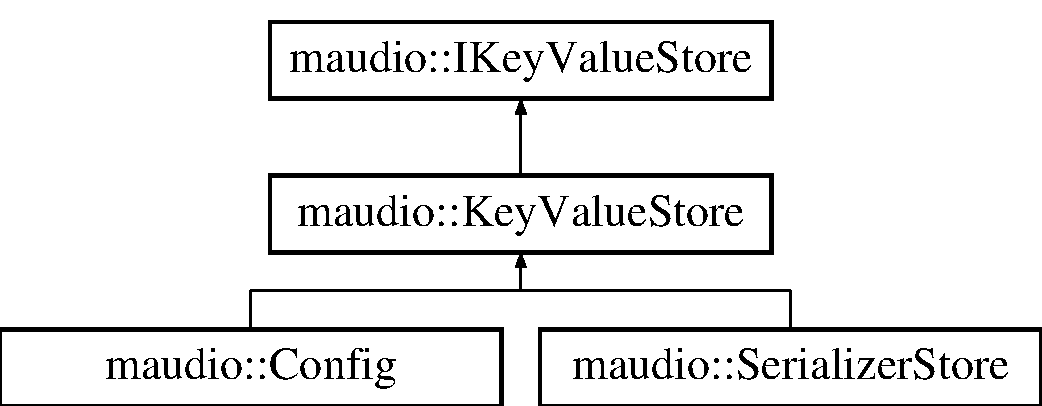
\includegraphics[height=3.000000cm]{classmaudio_1_1IKeyValueStore}
\end{center}
\end{figure}
\subsection*{Public Member Functions}
\begin{DoxyCompactItemize}
\item 
virtual \hyperlink{classmaudio_1_1IKeyValueStore_ac6e0f77db568079ad0a82a3c64058428}{$\sim$\-I\-Key\-Value\-Store} ()
\item 
virtual const char $\ast$ \hyperlink{classmaudio_1_1IKeyValueStore_a3d35bec96b6f1b4301b6ef5e03791181}{get} (const char $\ast$key) const =0
\item 
virtual const char $\ast$ \hyperlink{classmaudio_1_1IKeyValueStore_a06a7802cc710b2a30dabeabf65326d40}{get} (unsigned int num\-Key) const =0
\item 
virtual unsigned int \hyperlink{classmaudio_1_1IKeyValueStore_ac90d725769db3a9b56803e455dc086c4}{get\-Size} () const =0
\item 
virtual void \hyperlink{classmaudio_1_1IKeyValueStore_a6baf8502bc2d064d082eabe2072079de}{set} (const char $\ast$key, const char $\ast$value)=0
\end{DoxyCompactItemize}


\subsection{Constructor \& Destructor Documentation}
\hypertarget{classmaudio_1_1IKeyValueStore_ac6e0f77db568079ad0a82a3c64058428}{\index{maudio\-::\-I\-Key\-Value\-Store@{maudio\-::\-I\-Key\-Value\-Store}!$\sim$\-I\-Key\-Value\-Store@{$\sim$\-I\-Key\-Value\-Store}}
\index{$\sim$\-I\-Key\-Value\-Store@{$\sim$\-I\-Key\-Value\-Store}!maudio::IKeyValueStore@{maudio\-::\-I\-Key\-Value\-Store}}
\subsubsection[{$\sim$\-I\-Key\-Value\-Store}]{\setlength{\rightskip}{0pt plus 5cm}virtual maudio\-::\-I\-Key\-Value\-Store\-::$\sim$\-I\-Key\-Value\-Store (
\begin{DoxyParamCaption}
{}
\end{DoxyParamCaption}
)\hspace{0.3cm}{\ttfamily [inline]}, {\ttfamily [virtual]}}}\label{classmaudio_1_1IKeyValueStore_ac6e0f77db568079ad0a82a3c64058428}


\subsection{Member Function Documentation}
\hypertarget{classmaudio_1_1IKeyValueStore_a3d35bec96b6f1b4301b6ef5e03791181}{\index{maudio\-::\-I\-Key\-Value\-Store@{maudio\-::\-I\-Key\-Value\-Store}!get@{get}}
\index{get@{get}!maudio::IKeyValueStore@{maudio\-::\-I\-Key\-Value\-Store}}
\subsubsection[{get}]{\setlength{\rightskip}{0pt plus 5cm}virtual const char$\ast$ maudio\-::\-I\-Key\-Value\-Store\-::get (
\begin{DoxyParamCaption}
\item[{const char $\ast$}]{key}
\end{DoxyParamCaption}
) const\hspace{0.3cm}{\ttfamily [pure virtual]}}}\label{classmaudio_1_1IKeyValueStore_a3d35bec96b6f1b4301b6ef5e03791181}


Implemented in \hyperlink{classmaudio_1_1KeyValueStore_a21db38aeef23adde09a22eea9e85ab71}{maudio\-::\-Key\-Value\-Store}.

\hypertarget{classmaudio_1_1IKeyValueStore_a06a7802cc710b2a30dabeabf65326d40}{\index{maudio\-::\-I\-Key\-Value\-Store@{maudio\-::\-I\-Key\-Value\-Store}!get@{get}}
\index{get@{get}!maudio::IKeyValueStore@{maudio\-::\-I\-Key\-Value\-Store}}
\subsubsection[{get}]{\setlength{\rightskip}{0pt plus 5cm}virtual const char$\ast$ maudio\-::\-I\-Key\-Value\-Store\-::get (
\begin{DoxyParamCaption}
\item[{unsigned int}]{num\-Key}
\end{DoxyParamCaption}
) const\hspace{0.3cm}{\ttfamily [pure virtual]}}}\label{classmaudio_1_1IKeyValueStore_a06a7802cc710b2a30dabeabf65326d40}


Implemented in \hyperlink{classmaudio_1_1KeyValueStore_a5c9e0d1599466bd7895d87a587e1d909}{maudio\-::\-Key\-Value\-Store}, \hyperlink{classmaudio_1_1KeyValueStore_aaafd70f76ca552d5c221414cfb5f49cc}{maudio\-::\-Key\-Value\-Store}, and \hyperlink{classmaudio_1_1KeyValueStore_a0c19dbb4603a13e45d4c6a8c8b085758}{maudio\-::\-Key\-Value\-Store}.

\hypertarget{classmaudio_1_1IKeyValueStore_ac90d725769db3a9b56803e455dc086c4}{\index{maudio\-::\-I\-Key\-Value\-Store@{maudio\-::\-I\-Key\-Value\-Store}!get\-Size@{get\-Size}}
\index{get\-Size@{get\-Size}!maudio::IKeyValueStore@{maudio\-::\-I\-Key\-Value\-Store}}
\subsubsection[{get\-Size}]{\setlength{\rightskip}{0pt plus 5cm}virtual unsigned int maudio\-::\-I\-Key\-Value\-Store\-::get\-Size (
\begin{DoxyParamCaption}
{}
\end{DoxyParamCaption}
) const\hspace{0.3cm}{\ttfamily [pure virtual]}}}\label{classmaudio_1_1IKeyValueStore_ac90d725769db3a9b56803e455dc086c4}


Implemented in \hyperlink{classmaudio_1_1KeyValueStore_acb51935ff31c59168f72be8af784433a}{maudio\-::\-Key\-Value\-Store}.

\hypertarget{classmaudio_1_1IKeyValueStore_a6baf8502bc2d064d082eabe2072079de}{\index{maudio\-::\-I\-Key\-Value\-Store@{maudio\-::\-I\-Key\-Value\-Store}!set@{set}}
\index{set@{set}!maudio::IKeyValueStore@{maudio\-::\-I\-Key\-Value\-Store}}
\subsubsection[{set}]{\setlength{\rightskip}{0pt plus 5cm}virtual void maudio\-::\-I\-Key\-Value\-Store\-::set (
\begin{DoxyParamCaption}
\item[{const char $\ast$}]{key, }
\item[{const char $\ast$}]{value}
\end{DoxyParamCaption}
)\hspace{0.3cm}{\ttfamily [pure virtual]}}}\label{classmaudio_1_1IKeyValueStore_a6baf8502bc2d064d082eabe2072079de}


Implemented in \hyperlink{classmaudio_1_1KeyValueStore_a85374af3b968a7bfe7e3e11a9a228375}{maudio\-::\-Key\-Value\-Store}.



The documentation for this class was generated from the following file\-:\begin{DoxyCompactItemize}
\item 
/home/mars/\-Projekte/maudio/src/plugins/include/core/store/\hyperlink{IKeyValueStore_8hpp}{I\-Key\-Value\-Store.\-hpp}\end{DoxyCompactItemize}

\hypertarget{classmaudio_1_1InternalException}{\section{maudio\-:\-:Internal\-Exception Class Reference}
\label{classmaudio_1_1InternalException}\index{maudio\-::\-Internal\-Exception@{maudio\-::\-Internal\-Exception}}
}


{\ttfamily \#include $<$Audio\-Exception.\-hpp$>$}

Inheritance diagram for maudio\-:\-:Internal\-Exception\-:\begin{figure}[H]
\begin{center}
\leavevmode
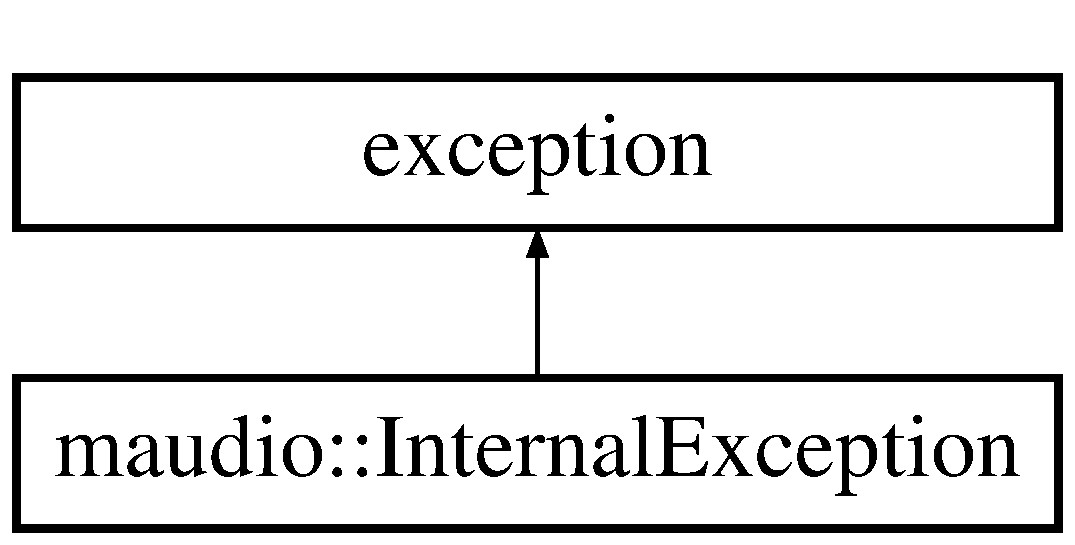
\includegraphics[height=2.000000cm]{classmaudio_1_1InternalException}
\end{center}
\end{figure}
\subsection*{Public Member Functions}
\begin{DoxyCompactItemize}
\item 
virtual const char $\ast$ \hyperlink{classmaudio_1_1InternalException_ab5d0a7ca2d0994a04958b76915853063}{what} () const   throw ()
\end{DoxyCompactItemize}


\subsection{Member Function Documentation}
\hypertarget{classmaudio_1_1InternalException_ab5d0a7ca2d0994a04958b76915853063}{\index{maudio\-::\-Internal\-Exception@{maudio\-::\-Internal\-Exception}!what@{what}}
\index{what@{what}!maudio::InternalException@{maudio\-::\-Internal\-Exception}}
\subsubsection[{what}]{\setlength{\rightskip}{0pt plus 5cm}virtual const char$\ast$ maudio\-::\-Internal\-Exception\-::what (
\begin{DoxyParamCaption}
{}
\end{DoxyParamCaption}
) const throw  ) \hspace{0.3cm}{\ttfamily [inline]}, {\ttfamily [virtual]}}}\label{classmaudio_1_1InternalException_ab5d0a7ca2d0994a04958b76915853063}


The documentation for this class was generated from the following file\-:\begin{DoxyCompactItemize}
\item 
/home/mars/\-Projekte/maudio/src/plugins/include/core/util/\hyperlink{AudioException_8hpp}{Audio\-Exception.\-hpp}\end{DoxyCompactItemize}

\hypertarget{classmaudio_1_1InvalidAudioDeviceException}{\section{maudio\-:\-:Invalid\-Audio\-Device\-Exception Class Reference}
\label{classmaudio_1_1InvalidAudioDeviceException}\index{maudio\-::\-Invalid\-Audio\-Device\-Exception@{maudio\-::\-Invalid\-Audio\-Device\-Exception}}
}


{\ttfamily \#include $<$Audio\-Exception.\-hpp$>$}

Inheritance diagram for maudio\-:\-:Invalid\-Audio\-Device\-Exception\-:\begin{figure}[H]
\begin{center}
\leavevmode
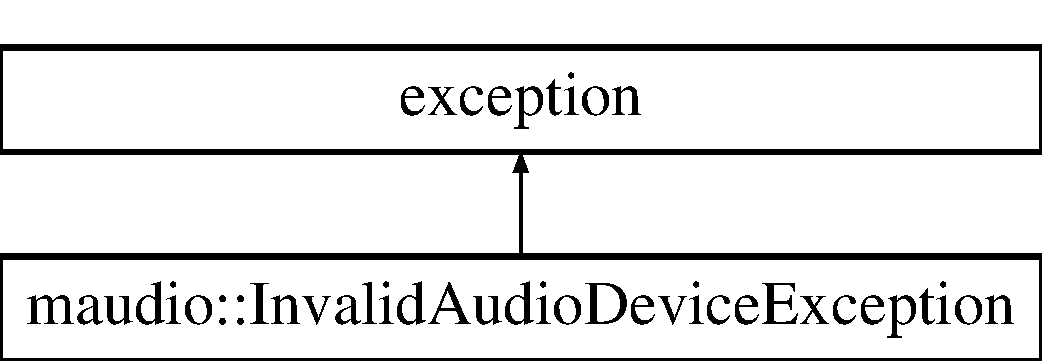
\includegraphics[height=2.000000cm]{classmaudio_1_1InvalidAudioDeviceException}
\end{center}
\end{figure}
\subsection*{Public Member Functions}
\begin{DoxyCompactItemize}
\item 
virtual const char $\ast$ \hyperlink{classmaudio_1_1InvalidAudioDeviceException_acff50bee3807e699d0ab84589fb3c519}{what} () const   throw ()
\end{DoxyCompactItemize}


\subsection{Member Function Documentation}
\hypertarget{classmaudio_1_1InvalidAudioDeviceException_acff50bee3807e699d0ab84589fb3c519}{\index{maudio\-::\-Invalid\-Audio\-Device\-Exception@{maudio\-::\-Invalid\-Audio\-Device\-Exception}!what@{what}}
\index{what@{what}!maudio::InvalidAudioDeviceException@{maudio\-::\-Invalid\-Audio\-Device\-Exception}}
\subsubsection[{what}]{\setlength{\rightskip}{0pt plus 5cm}virtual const char$\ast$ maudio\-::\-Invalid\-Audio\-Device\-Exception\-::what (
\begin{DoxyParamCaption}
{}
\end{DoxyParamCaption}
) const throw  ) \hspace{0.3cm}{\ttfamily [inline]}, {\ttfamily [virtual]}}}\label{classmaudio_1_1InvalidAudioDeviceException_acff50bee3807e699d0ab84589fb3c519}


The documentation for this class was generated from the following file\-:\begin{DoxyCompactItemize}
\item 
/home/mars/\-Projekte/maudio/src/plugins/include/core/util/\hyperlink{AudioException_8hpp}{Audio\-Exception.\-hpp}\end{DoxyCompactItemize}

\hypertarget{classmaudio_1_1InvalidDataException}{\section{maudio\-:\-:Invalid\-Data\-Exception Class Reference}
\label{classmaudio_1_1InvalidDataException}\index{maudio\-::\-Invalid\-Data\-Exception@{maudio\-::\-Invalid\-Data\-Exception}}
}


{\ttfamily \#include $<$Audio\-Exception.\-hpp$>$}

Inheritance diagram for maudio\-:\-:Invalid\-Data\-Exception\-:\begin{figure}[H]
\begin{center}
\leavevmode
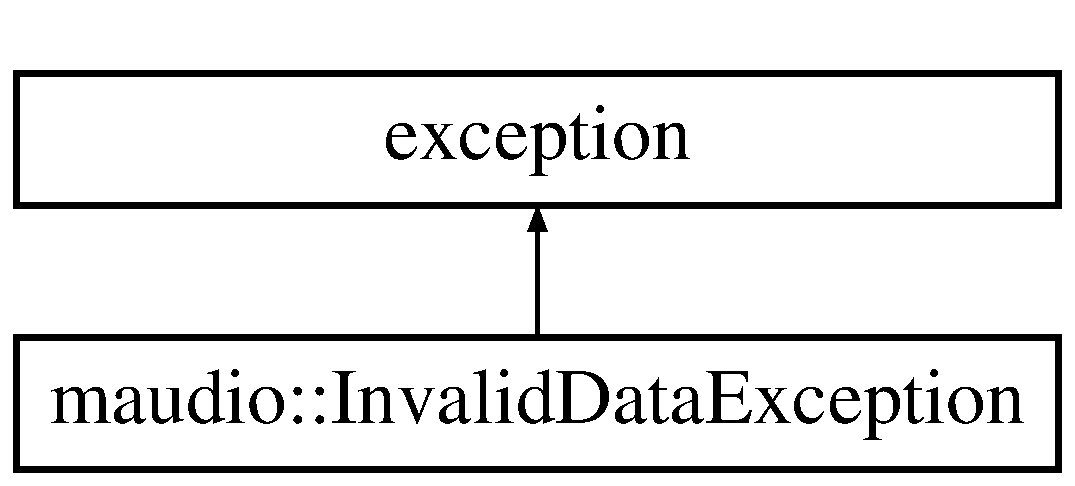
\includegraphics[height=2.000000cm]{classmaudio_1_1InvalidDataException}
\end{center}
\end{figure}
\subsection*{Public Member Functions}
\begin{DoxyCompactItemize}
\item 
virtual const char $\ast$ \hyperlink{classmaudio_1_1InvalidDataException_ab1fa1e9dcc9966530c84e4cded835055}{what} () const   throw ()
\end{DoxyCompactItemize}


\subsection{Member Function Documentation}
\hypertarget{classmaudio_1_1InvalidDataException_ab1fa1e9dcc9966530c84e4cded835055}{\index{maudio\-::\-Invalid\-Data\-Exception@{maudio\-::\-Invalid\-Data\-Exception}!what@{what}}
\index{what@{what}!maudio::InvalidDataException@{maudio\-::\-Invalid\-Data\-Exception}}
\subsubsection[{what}]{\setlength{\rightskip}{0pt plus 5cm}virtual const char$\ast$ maudio\-::\-Invalid\-Data\-Exception\-::what (
\begin{DoxyParamCaption}
{}
\end{DoxyParamCaption}
) const throw  ) \hspace{0.3cm}{\ttfamily [inline]}, {\ttfamily [virtual]}}}\label{classmaudio_1_1InvalidDataException_ab1fa1e9dcc9966530c84e4cded835055}


The documentation for this class was generated from the following file\-:\begin{DoxyCompactItemize}
\item 
/home/mars/\-Projekte/maudio/src/plugins/include/core/util/\hyperlink{AudioException_8hpp}{Audio\-Exception.\-hpp}\end{DoxyCompactItemize}

\hypertarget{classmaudio_1_1IProperty}{\section{maudio\-:\-:I\-Property Class Reference}
\label{classmaudio_1_1IProperty}\index{maudio\-::\-I\-Property@{maudio\-::\-I\-Property}}
}


{\ttfamily \#include $<$I\-Property.\-hpp$>$}

Inheritance diagram for maudio\-:\-:I\-Property\-:\begin{figure}[H]
\begin{center}
\leavevmode
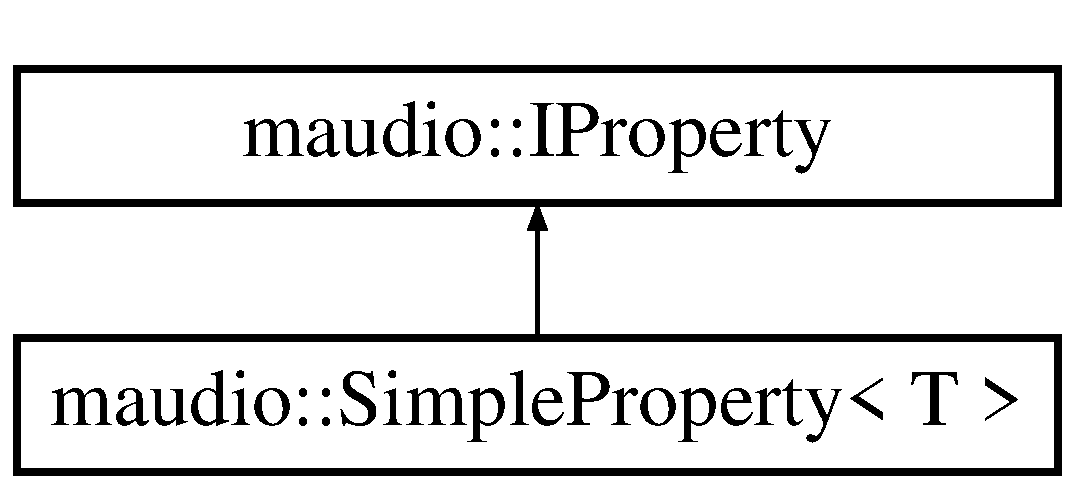
\includegraphics[height=2.000000cm]{classmaudio_1_1IProperty}
\end{center}
\end{figure}
\subsection*{Public Member Functions}
\begin{DoxyCompactItemize}
\item 
virtual \hyperlink{classmaudio_1_1IProperty_ab69580c42419d350dc2e0f8333e6d7c9}{$\sim$\-I\-Property} ()
\item 
virtual const char $\ast$ \hyperlink{classmaudio_1_1IProperty_a7964046c2be4eceb88021f0ab059f159}{get\-String} () const =0
\item 
virtual void \hyperlink{classmaudio_1_1IProperty_aeb474ef1dd68fd14d88de535eff92d0f}{set} (const char $\ast$value)=0
\item 
virtual const char $\ast$ \hyperlink{classmaudio_1_1IProperty_a6f859515ff25325a8a1eb32e76e4e66d}{get\-Name} () const =0
\item 
virtual const char $\ast$ \hyperlink{classmaudio_1_1IProperty_af82e89808ac54aee7a92c182b0ac9e5d}{get\-Bottom\-Bounds\-String} () const =0
\item 
virtual const char $\ast$ \hyperlink{classmaudio_1_1IProperty_a4182ebf0441cf1d3927e222331f00e93}{get\-Upper\-Bounds\-String} () const =0
\end{DoxyCompactItemize}


\subsection{Constructor \& Destructor Documentation}
\hypertarget{classmaudio_1_1IProperty_ab69580c42419d350dc2e0f8333e6d7c9}{\index{maudio\-::\-I\-Property@{maudio\-::\-I\-Property}!$\sim$\-I\-Property@{$\sim$\-I\-Property}}
\index{$\sim$\-I\-Property@{$\sim$\-I\-Property}!maudio::IProperty@{maudio\-::\-I\-Property}}
\subsubsection[{$\sim$\-I\-Property}]{\setlength{\rightskip}{0pt plus 5cm}virtual maudio\-::\-I\-Property\-::$\sim$\-I\-Property (
\begin{DoxyParamCaption}
{}
\end{DoxyParamCaption}
)\hspace{0.3cm}{\ttfamily [inline]}, {\ttfamily [virtual]}}}\label{classmaudio_1_1IProperty_ab69580c42419d350dc2e0f8333e6d7c9}


\subsection{Member Function Documentation}
\hypertarget{classmaudio_1_1IProperty_af82e89808ac54aee7a92c182b0ac9e5d}{\index{maudio\-::\-I\-Property@{maudio\-::\-I\-Property}!get\-Bottom\-Bounds\-String@{get\-Bottom\-Bounds\-String}}
\index{get\-Bottom\-Bounds\-String@{get\-Bottom\-Bounds\-String}!maudio::IProperty@{maudio\-::\-I\-Property}}
\subsubsection[{get\-Bottom\-Bounds\-String}]{\setlength{\rightskip}{0pt plus 5cm}virtual const char$\ast$ maudio\-::\-I\-Property\-::get\-Bottom\-Bounds\-String (
\begin{DoxyParamCaption}
{}
\end{DoxyParamCaption}
) const\hspace{0.3cm}{\ttfamily [pure virtual]}}}\label{classmaudio_1_1IProperty_af82e89808ac54aee7a92c182b0ac9e5d}


Implemented in \hyperlink{classmaudio_1_1SimpleProperty_a6e0133f2b112033ce7519d2f32d913d4}{maudio\-::\-Simple\-Property$<$ T $>$}.

\hypertarget{classmaudio_1_1IProperty_a6f859515ff25325a8a1eb32e76e4e66d}{\index{maudio\-::\-I\-Property@{maudio\-::\-I\-Property}!get\-Name@{get\-Name}}
\index{get\-Name@{get\-Name}!maudio::IProperty@{maudio\-::\-I\-Property}}
\subsubsection[{get\-Name}]{\setlength{\rightskip}{0pt plus 5cm}virtual const char$\ast$ maudio\-::\-I\-Property\-::get\-Name (
\begin{DoxyParamCaption}
{}
\end{DoxyParamCaption}
) const\hspace{0.3cm}{\ttfamily [pure virtual]}}}\label{classmaudio_1_1IProperty_a6f859515ff25325a8a1eb32e76e4e66d}


Implemented in \hyperlink{classmaudio_1_1SimpleProperty_aafd58fa45a18b7b302d526ff267d9db2}{maudio\-::\-Simple\-Property$<$ T $>$}.

\hypertarget{classmaudio_1_1IProperty_a7964046c2be4eceb88021f0ab059f159}{\index{maudio\-::\-I\-Property@{maudio\-::\-I\-Property}!get\-String@{get\-String}}
\index{get\-String@{get\-String}!maudio::IProperty@{maudio\-::\-I\-Property}}
\subsubsection[{get\-String}]{\setlength{\rightskip}{0pt plus 5cm}virtual const char$\ast$ maudio\-::\-I\-Property\-::get\-String (
\begin{DoxyParamCaption}
{}
\end{DoxyParamCaption}
) const\hspace{0.3cm}{\ttfamily [pure virtual]}}}\label{classmaudio_1_1IProperty_a7964046c2be4eceb88021f0ab059f159}


Implemented in \hyperlink{classmaudio_1_1SimpleProperty_a12036db02a41a82e49d21a200b04e8b0}{maudio\-::\-Simple\-Property$<$ T $>$}, \hyperlink{classmaudio_1_1SimpleProperty_a3033164121186a18c5e4bef19bf939de}{maudio\-::\-Simple\-Property$<$ T $>$}, and \hyperlink{classmaudio_1_1SimpleProperty_a3033164121186a18c5e4bef19bf939de}{maudio\-::\-Simple\-Property$<$ T $>$}.

\hypertarget{classmaudio_1_1IProperty_a4182ebf0441cf1d3927e222331f00e93}{\index{maudio\-::\-I\-Property@{maudio\-::\-I\-Property}!get\-Upper\-Bounds\-String@{get\-Upper\-Bounds\-String}}
\index{get\-Upper\-Bounds\-String@{get\-Upper\-Bounds\-String}!maudio::IProperty@{maudio\-::\-I\-Property}}
\subsubsection[{get\-Upper\-Bounds\-String}]{\setlength{\rightskip}{0pt plus 5cm}virtual const char$\ast$ maudio\-::\-I\-Property\-::get\-Upper\-Bounds\-String (
\begin{DoxyParamCaption}
{}
\end{DoxyParamCaption}
) const\hspace{0.3cm}{\ttfamily [pure virtual]}}}\label{classmaudio_1_1IProperty_a4182ebf0441cf1d3927e222331f00e93}


Implemented in \hyperlink{classmaudio_1_1SimpleProperty_ac5ccd635686253991acf57d8a2ddbeca}{maudio\-::\-Simple\-Property$<$ T $>$}.

\hypertarget{classmaudio_1_1IProperty_aeb474ef1dd68fd14d88de535eff92d0f}{\index{maudio\-::\-I\-Property@{maudio\-::\-I\-Property}!set@{set}}
\index{set@{set}!maudio::IProperty@{maudio\-::\-I\-Property}}
\subsubsection[{set}]{\setlength{\rightskip}{0pt plus 5cm}virtual void maudio\-::\-I\-Property\-::set (
\begin{DoxyParamCaption}
\item[{const char $\ast$}]{value}
\end{DoxyParamCaption}
)\hspace{0.3cm}{\ttfamily [pure virtual]}}}\label{classmaudio_1_1IProperty_aeb474ef1dd68fd14d88de535eff92d0f}


Implemented in \hyperlink{classmaudio_1_1SimpleProperty_a8edb07f2fd51fd60c43a6f35ef45342b}{maudio\-::\-Simple\-Property$<$ T $>$}.



The documentation for this class was generated from the following file\-:\begin{DoxyCompactItemize}
\item 
/home/mars/\-Projekte/maudio/src/plugins/include/core/property/\hyperlink{IProperty_8hpp}{I\-Property.\-hpp}\end{DoxyCompactItemize}

\hypertarget{classmaudio_1_1IPropertyManager}{\section{maudio\-:\-:I\-Property\-Manager Class Reference}
\label{classmaudio_1_1IPropertyManager}\index{maudio\-::\-I\-Property\-Manager@{maudio\-::\-I\-Property\-Manager}}
}


{\ttfamily \#include $<$I\-Property\-Manager.\-hpp$>$}

Inheritance diagram for maudio\-:\-:I\-Property\-Manager\-:\begin{figure}[H]
\begin{center}
\leavevmode
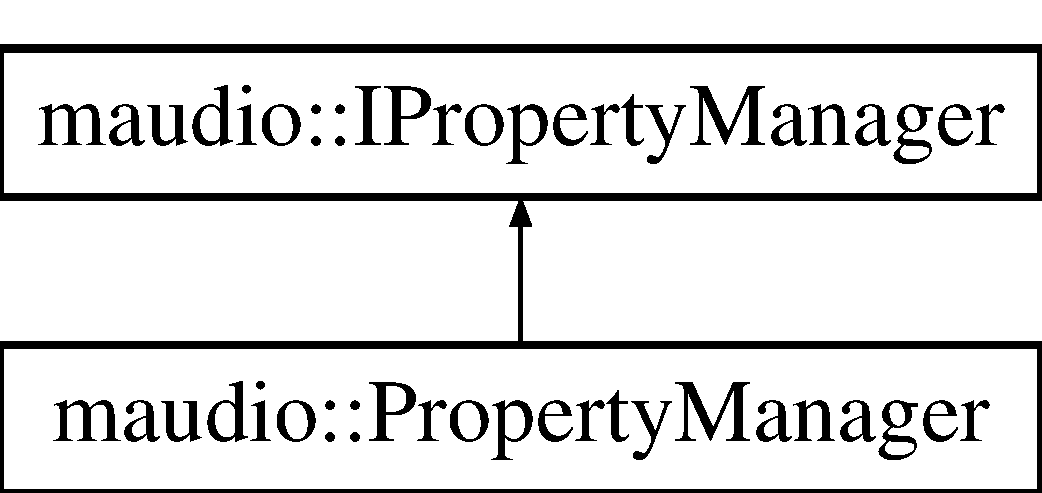
\includegraphics[height=2.000000cm]{classmaudio_1_1IPropertyManager}
\end{center}
\end{figure}
\subsection*{Public Member Functions}
\begin{DoxyCompactItemize}
\item 
virtual \hyperlink{classmaudio_1_1IPropertyManager_a6d20a85da5ef123b1ccd72360c5d24e4}{$\sim$\-I\-Property\-Manager} ()
\item 
virtual void \hyperlink{classmaudio_1_1IPropertyManager_a6f1c1a5a3e9714e8ab22b73a5f67807e}{add} (\hyperlink{classmaudio_1_1IProperty}{I\-Property} $\ast$prop)=0
\item 
virtual void \hyperlink{classmaudio_1_1IPropertyManager_a719bb2f8d8fb55126c7dc6d264600768}{add} (\hyperlink{classmaudio_1_1IKeyableProperty}{I\-Keyable\-Property} $\ast$prop)=0
\item 
virtual bool \hyperlink{classmaudio_1_1IPropertyManager_a0d2b0d87656c2eb7e93ca867848d1559}{Property\-Exists} (const char $\ast$name)=0
\item 
virtual bool \hyperlink{classmaudio_1_1IPropertyManager_a95f90f98cff9992a48fabe61168c95fb}{Keyable\-Property\-Exists} (const char $\ast$name)=0
\item 
virtual \hyperlink{classmaudio_1_1IProperty}{I\-Property} $\ast$ \hyperlink{classmaudio_1_1IPropertyManager_af25154a1f612b2bc44e40304290615ef}{get\-Property} (unsigned int i)=0
\item 
virtual \hyperlink{classmaudio_1_1IProperty}{I\-Property} $\ast$ \hyperlink{classmaudio_1_1IPropertyManager_acbaea1cbdc990b9b4b0416a5c35d9435}{get\-Property} (const char $\ast$name)=0
\item 
virtual \hyperlink{classmaudio_1_1IKeyableProperty}{I\-Keyable\-Property} $\ast$ \hyperlink{classmaudio_1_1IPropertyManager_a68747539c9a666215de88337998b45d7}{get\-Keyable\-Property} (unsigned int i)=0
\item 
virtual \hyperlink{classmaudio_1_1IKeyableProperty}{I\-Keyable\-Property} $\ast$ \hyperlink{classmaudio_1_1IPropertyManager_ac53ff45a9a42e265fa0d044a09bcc2ae}{get\-Keyable\-Property} (const char $\ast$name)=0
\item 
virtual void \hyperlink{classmaudio_1_1IPropertyManager_aedc3df4a29c0ae8d137ac29b5b0abbf1}{remove\-Property} (unsigned int i)=0
\item 
virtual void \hyperlink{classmaudio_1_1IPropertyManager_a41d9333efef184d05a1e1c929097059f}{remove\-Property} (const char $\ast$name)=0
\item 
virtual void \hyperlink{classmaudio_1_1IPropertyManager_a6fbce7ab4d22a147fba13d54be8c6328}{remove\-Keyable\-Property} (unsigned int i)=0
\item 
virtual void \hyperlink{classmaudio_1_1IPropertyManager_a31ab51fa15263b7aa67a6a0dd1f91985}{remove\-Keyable\-Property} (const char $\ast$name)=0
\item 
virtual unsigned int \hyperlink{classmaudio_1_1IPropertyManager_a27d2e238fc13c322941a21ef0c2aa04a}{get\-Num\-Properties} () const =0
\item 
virtual unsigned int \hyperlink{classmaudio_1_1IPropertyManager_a7f7f9bab86f9972dadc0313589a2f07a}{get\-Num\-Keyable\-Properties} () const =0
\end{DoxyCompactItemize}


\subsection{Constructor \& Destructor Documentation}
\hypertarget{classmaudio_1_1IPropertyManager_a6d20a85da5ef123b1ccd72360c5d24e4}{\index{maudio\-::\-I\-Property\-Manager@{maudio\-::\-I\-Property\-Manager}!$\sim$\-I\-Property\-Manager@{$\sim$\-I\-Property\-Manager}}
\index{$\sim$\-I\-Property\-Manager@{$\sim$\-I\-Property\-Manager}!maudio::IPropertyManager@{maudio\-::\-I\-Property\-Manager}}
\subsubsection[{$\sim$\-I\-Property\-Manager}]{\setlength{\rightskip}{0pt plus 5cm}virtual maudio\-::\-I\-Property\-Manager\-::$\sim$\-I\-Property\-Manager (
\begin{DoxyParamCaption}
{}
\end{DoxyParamCaption}
)\hspace{0.3cm}{\ttfamily [inline]}, {\ttfamily [virtual]}}}\label{classmaudio_1_1IPropertyManager_a6d20a85da5ef123b1ccd72360c5d24e4}


\subsection{Member Function Documentation}
\hypertarget{classmaudio_1_1IPropertyManager_a6f1c1a5a3e9714e8ab22b73a5f67807e}{\index{maudio\-::\-I\-Property\-Manager@{maudio\-::\-I\-Property\-Manager}!add@{add}}
\index{add@{add}!maudio::IPropertyManager@{maudio\-::\-I\-Property\-Manager}}
\subsubsection[{add}]{\setlength{\rightskip}{0pt plus 5cm}virtual void maudio\-::\-I\-Property\-Manager\-::add (
\begin{DoxyParamCaption}
\item[{{\bf I\-Property} $\ast$}]{prop}
\end{DoxyParamCaption}
)\hspace{0.3cm}{\ttfamily [pure virtual]}}}\label{classmaudio_1_1IPropertyManager_a6f1c1a5a3e9714e8ab22b73a5f67807e}


Implemented in \hyperlink{classmaudio_1_1PropertyManager_a247f345f6b91df3269d0032a7eadc78d}{maudio\-::\-Property\-Manager}.

\hypertarget{classmaudio_1_1IPropertyManager_a719bb2f8d8fb55126c7dc6d264600768}{\index{maudio\-::\-I\-Property\-Manager@{maudio\-::\-I\-Property\-Manager}!add@{add}}
\index{add@{add}!maudio::IPropertyManager@{maudio\-::\-I\-Property\-Manager}}
\subsubsection[{add}]{\setlength{\rightskip}{0pt plus 5cm}virtual void maudio\-::\-I\-Property\-Manager\-::add (
\begin{DoxyParamCaption}
\item[{{\bf I\-Keyable\-Property} $\ast$}]{prop}
\end{DoxyParamCaption}
)\hspace{0.3cm}{\ttfamily [pure virtual]}}}\label{classmaudio_1_1IPropertyManager_a719bb2f8d8fb55126c7dc6d264600768}


Implemented in \hyperlink{classmaudio_1_1PropertyManager_a01820518f68793e5c2f9a2720b962bae}{maudio\-::\-Property\-Manager}.

\hypertarget{classmaudio_1_1IPropertyManager_a68747539c9a666215de88337998b45d7}{\index{maudio\-::\-I\-Property\-Manager@{maudio\-::\-I\-Property\-Manager}!get\-Keyable\-Property@{get\-Keyable\-Property}}
\index{get\-Keyable\-Property@{get\-Keyable\-Property}!maudio::IPropertyManager@{maudio\-::\-I\-Property\-Manager}}
\subsubsection[{get\-Keyable\-Property}]{\setlength{\rightskip}{0pt plus 5cm}virtual {\bf I\-Keyable\-Property}$\ast$ maudio\-::\-I\-Property\-Manager\-::get\-Keyable\-Property (
\begin{DoxyParamCaption}
\item[{unsigned int}]{i}
\end{DoxyParamCaption}
)\hspace{0.3cm}{\ttfamily [pure virtual]}}}\label{classmaudio_1_1IPropertyManager_a68747539c9a666215de88337998b45d7}


Implemented in \hyperlink{classmaudio_1_1PropertyManager_a6e1fe28a2f4d92cde3f3bb0d60ce4666}{maudio\-::\-Property\-Manager}.

\hypertarget{classmaudio_1_1IPropertyManager_ac53ff45a9a42e265fa0d044a09bcc2ae}{\index{maudio\-::\-I\-Property\-Manager@{maudio\-::\-I\-Property\-Manager}!get\-Keyable\-Property@{get\-Keyable\-Property}}
\index{get\-Keyable\-Property@{get\-Keyable\-Property}!maudio::IPropertyManager@{maudio\-::\-I\-Property\-Manager}}
\subsubsection[{get\-Keyable\-Property}]{\setlength{\rightskip}{0pt plus 5cm}virtual {\bf I\-Keyable\-Property}$\ast$ maudio\-::\-I\-Property\-Manager\-::get\-Keyable\-Property (
\begin{DoxyParamCaption}
\item[{const char $\ast$}]{name}
\end{DoxyParamCaption}
)\hspace{0.3cm}{\ttfamily [pure virtual]}}}\label{classmaudio_1_1IPropertyManager_ac53ff45a9a42e265fa0d044a09bcc2ae}


Implemented in \hyperlink{classmaudio_1_1PropertyManager_a5c9dbb27aef129bb1f23fb1d2eca6af3}{maudio\-::\-Property\-Manager}.

\hypertarget{classmaudio_1_1IPropertyManager_a7f7f9bab86f9972dadc0313589a2f07a}{\index{maudio\-::\-I\-Property\-Manager@{maudio\-::\-I\-Property\-Manager}!get\-Num\-Keyable\-Properties@{get\-Num\-Keyable\-Properties}}
\index{get\-Num\-Keyable\-Properties@{get\-Num\-Keyable\-Properties}!maudio::IPropertyManager@{maudio\-::\-I\-Property\-Manager}}
\subsubsection[{get\-Num\-Keyable\-Properties}]{\setlength{\rightskip}{0pt plus 5cm}virtual unsigned int maudio\-::\-I\-Property\-Manager\-::get\-Num\-Keyable\-Properties (
\begin{DoxyParamCaption}
{}
\end{DoxyParamCaption}
) const\hspace{0.3cm}{\ttfamily [pure virtual]}}}\label{classmaudio_1_1IPropertyManager_a7f7f9bab86f9972dadc0313589a2f07a}


Implemented in \hyperlink{classmaudio_1_1PropertyManager_a27309f637c4ab28f45c1cd57381701d4}{maudio\-::\-Property\-Manager}.

\hypertarget{classmaudio_1_1IPropertyManager_a27d2e238fc13c322941a21ef0c2aa04a}{\index{maudio\-::\-I\-Property\-Manager@{maudio\-::\-I\-Property\-Manager}!get\-Num\-Properties@{get\-Num\-Properties}}
\index{get\-Num\-Properties@{get\-Num\-Properties}!maudio::IPropertyManager@{maudio\-::\-I\-Property\-Manager}}
\subsubsection[{get\-Num\-Properties}]{\setlength{\rightskip}{0pt plus 5cm}virtual unsigned int maudio\-::\-I\-Property\-Manager\-::get\-Num\-Properties (
\begin{DoxyParamCaption}
{}
\end{DoxyParamCaption}
) const\hspace{0.3cm}{\ttfamily [pure virtual]}}}\label{classmaudio_1_1IPropertyManager_a27d2e238fc13c322941a21ef0c2aa04a}


Implemented in \hyperlink{classmaudio_1_1PropertyManager_a12bec217f1ba5d9c0dfd2c9d872f5701}{maudio\-::\-Property\-Manager}.

\hypertarget{classmaudio_1_1IPropertyManager_af25154a1f612b2bc44e40304290615ef}{\index{maudio\-::\-I\-Property\-Manager@{maudio\-::\-I\-Property\-Manager}!get\-Property@{get\-Property}}
\index{get\-Property@{get\-Property}!maudio::IPropertyManager@{maudio\-::\-I\-Property\-Manager}}
\subsubsection[{get\-Property}]{\setlength{\rightskip}{0pt plus 5cm}virtual {\bf I\-Property}$\ast$ maudio\-::\-I\-Property\-Manager\-::get\-Property (
\begin{DoxyParamCaption}
\item[{unsigned int}]{i}
\end{DoxyParamCaption}
)\hspace{0.3cm}{\ttfamily [pure virtual]}}}\label{classmaudio_1_1IPropertyManager_af25154a1f612b2bc44e40304290615ef}


Implemented in \hyperlink{classmaudio_1_1PropertyManager_ad2d108b698b9e61f881670a9f5ce5132}{maudio\-::\-Property\-Manager}.

\hypertarget{classmaudio_1_1IPropertyManager_acbaea1cbdc990b9b4b0416a5c35d9435}{\index{maudio\-::\-I\-Property\-Manager@{maudio\-::\-I\-Property\-Manager}!get\-Property@{get\-Property}}
\index{get\-Property@{get\-Property}!maudio::IPropertyManager@{maudio\-::\-I\-Property\-Manager}}
\subsubsection[{get\-Property}]{\setlength{\rightskip}{0pt plus 5cm}virtual {\bf I\-Property}$\ast$ maudio\-::\-I\-Property\-Manager\-::get\-Property (
\begin{DoxyParamCaption}
\item[{const char $\ast$}]{name}
\end{DoxyParamCaption}
)\hspace{0.3cm}{\ttfamily [pure virtual]}}}\label{classmaudio_1_1IPropertyManager_acbaea1cbdc990b9b4b0416a5c35d9435}


Implemented in \hyperlink{classmaudio_1_1PropertyManager_ab947ffa97971be8b44047d444a99c65f}{maudio\-::\-Property\-Manager}.

\hypertarget{classmaudio_1_1IPropertyManager_a95f90f98cff9992a48fabe61168c95fb}{\index{maudio\-::\-I\-Property\-Manager@{maudio\-::\-I\-Property\-Manager}!Keyable\-Property\-Exists@{Keyable\-Property\-Exists}}
\index{Keyable\-Property\-Exists@{Keyable\-Property\-Exists}!maudio::IPropertyManager@{maudio\-::\-I\-Property\-Manager}}
\subsubsection[{Keyable\-Property\-Exists}]{\setlength{\rightskip}{0pt plus 5cm}virtual bool maudio\-::\-I\-Property\-Manager\-::\-Keyable\-Property\-Exists (
\begin{DoxyParamCaption}
\item[{const char $\ast$}]{name}
\end{DoxyParamCaption}
)\hspace{0.3cm}{\ttfamily [pure virtual]}}}\label{classmaudio_1_1IPropertyManager_a95f90f98cff9992a48fabe61168c95fb}


Implemented in \hyperlink{classmaudio_1_1PropertyManager_a2d21e0f5b613771d721d21e35d30dca2}{maudio\-::\-Property\-Manager}.

\hypertarget{classmaudio_1_1IPropertyManager_a0d2b0d87656c2eb7e93ca867848d1559}{\index{maudio\-::\-I\-Property\-Manager@{maudio\-::\-I\-Property\-Manager}!Property\-Exists@{Property\-Exists}}
\index{Property\-Exists@{Property\-Exists}!maudio::IPropertyManager@{maudio\-::\-I\-Property\-Manager}}
\subsubsection[{Property\-Exists}]{\setlength{\rightskip}{0pt plus 5cm}virtual bool maudio\-::\-I\-Property\-Manager\-::\-Property\-Exists (
\begin{DoxyParamCaption}
\item[{const char $\ast$}]{name}
\end{DoxyParamCaption}
)\hspace{0.3cm}{\ttfamily [pure virtual]}}}\label{classmaudio_1_1IPropertyManager_a0d2b0d87656c2eb7e93ca867848d1559}


Implemented in \hyperlink{classmaudio_1_1PropertyManager_a0bb59c88f642ec5d24fa3c1c991378ed}{maudio\-::\-Property\-Manager}.

\hypertarget{classmaudio_1_1IPropertyManager_a6fbce7ab4d22a147fba13d54be8c6328}{\index{maudio\-::\-I\-Property\-Manager@{maudio\-::\-I\-Property\-Manager}!remove\-Keyable\-Property@{remove\-Keyable\-Property}}
\index{remove\-Keyable\-Property@{remove\-Keyable\-Property}!maudio::IPropertyManager@{maudio\-::\-I\-Property\-Manager}}
\subsubsection[{remove\-Keyable\-Property}]{\setlength{\rightskip}{0pt plus 5cm}virtual void maudio\-::\-I\-Property\-Manager\-::remove\-Keyable\-Property (
\begin{DoxyParamCaption}
\item[{unsigned int}]{i}
\end{DoxyParamCaption}
)\hspace{0.3cm}{\ttfamily [pure virtual]}}}\label{classmaudio_1_1IPropertyManager_a6fbce7ab4d22a147fba13d54be8c6328}


Implemented in \hyperlink{classmaudio_1_1PropertyManager_a15c0a2e042acc6170631c2139785eae6}{maudio\-::\-Property\-Manager}.

\hypertarget{classmaudio_1_1IPropertyManager_a31ab51fa15263b7aa67a6a0dd1f91985}{\index{maudio\-::\-I\-Property\-Manager@{maudio\-::\-I\-Property\-Manager}!remove\-Keyable\-Property@{remove\-Keyable\-Property}}
\index{remove\-Keyable\-Property@{remove\-Keyable\-Property}!maudio::IPropertyManager@{maudio\-::\-I\-Property\-Manager}}
\subsubsection[{remove\-Keyable\-Property}]{\setlength{\rightskip}{0pt plus 5cm}virtual void maudio\-::\-I\-Property\-Manager\-::remove\-Keyable\-Property (
\begin{DoxyParamCaption}
\item[{const char $\ast$}]{name}
\end{DoxyParamCaption}
)\hspace{0.3cm}{\ttfamily [pure virtual]}}}\label{classmaudio_1_1IPropertyManager_a31ab51fa15263b7aa67a6a0dd1f91985}


Implemented in \hyperlink{classmaudio_1_1PropertyManager_afc5d658aa68cb326e60225818d128a89}{maudio\-::\-Property\-Manager}.

\hypertarget{classmaudio_1_1IPropertyManager_aedc3df4a29c0ae8d137ac29b5b0abbf1}{\index{maudio\-::\-I\-Property\-Manager@{maudio\-::\-I\-Property\-Manager}!remove\-Property@{remove\-Property}}
\index{remove\-Property@{remove\-Property}!maudio::IPropertyManager@{maudio\-::\-I\-Property\-Manager}}
\subsubsection[{remove\-Property}]{\setlength{\rightskip}{0pt plus 5cm}virtual void maudio\-::\-I\-Property\-Manager\-::remove\-Property (
\begin{DoxyParamCaption}
\item[{unsigned int}]{i}
\end{DoxyParamCaption}
)\hspace{0.3cm}{\ttfamily [pure virtual]}}}\label{classmaudio_1_1IPropertyManager_aedc3df4a29c0ae8d137ac29b5b0abbf1}


Implemented in \hyperlink{classmaudio_1_1PropertyManager_aa4dc70e93cf8f59275ed25c1bcaa804c}{maudio\-::\-Property\-Manager}.

\hypertarget{classmaudio_1_1IPropertyManager_a41d9333efef184d05a1e1c929097059f}{\index{maudio\-::\-I\-Property\-Manager@{maudio\-::\-I\-Property\-Manager}!remove\-Property@{remove\-Property}}
\index{remove\-Property@{remove\-Property}!maudio::IPropertyManager@{maudio\-::\-I\-Property\-Manager}}
\subsubsection[{remove\-Property}]{\setlength{\rightskip}{0pt plus 5cm}virtual void maudio\-::\-I\-Property\-Manager\-::remove\-Property (
\begin{DoxyParamCaption}
\item[{const char $\ast$}]{name}
\end{DoxyParamCaption}
)\hspace{0.3cm}{\ttfamily [pure virtual]}}}\label{classmaudio_1_1IPropertyManager_a41d9333efef184d05a1e1c929097059f}


Implemented in \hyperlink{classmaudio_1_1PropertyManager_a737ebb28d24c575ecff05c81556f0ae1}{maudio\-::\-Property\-Manager}.



The documentation for this class was generated from the following file\-:\begin{DoxyCompactItemize}
\item 
/home/mars/\-Projekte/maudio/src/plugins/include/core/property/\hyperlink{IPropertyManager_8hpp}{I\-Property\-Manager.\-hpp}\end{DoxyCompactItemize}

\hypertarget{classmaudio_1_1ISample}{\section{maudio\-:\-:I\-Sample Class Reference}
\label{classmaudio_1_1ISample}\index{maudio\-::\-I\-Sample@{maudio\-::\-I\-Sample}}
}


Holds a sample of audio.  




{\ttfamily \#include $<$I\-Sample.\-hpp$>$}

Inheritance diagram for maudio\-:\-:I\-Sample\-:\begin{figure}[H]
\begin{center}
\leavevmode
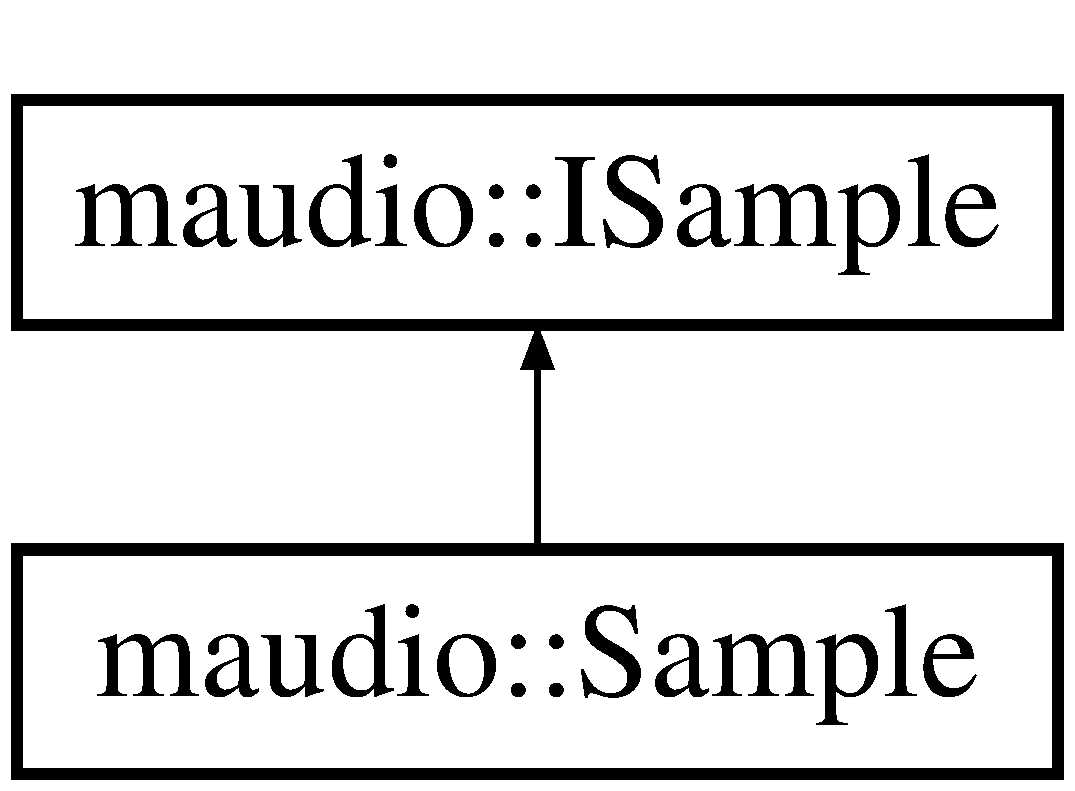
\includegraphics[height=2.000000cm]{classmaudio_1_1ISample}
\end{center}
\end{figure}
\subsection*{Public Member Functions}
\begin{DoxyCompactItemize}
\item 
virtual \hyperlink{classmaudio_1_1ISample_ad4b8a6224f76943f9a10e6d5bb16a1fd}{$\sim$\-I\-Sample} ()
\item 
virtual const float \hyperlink{classmaudio_1_1ISample_ad90962cd3f480cbba7a891530371e405}{operator\mbox{[}$\,$\mbox{]}} (unsigned int pos) const =0
\item 
virtual float \hyperlink{classmaudio_1_1ISample_a2a1eef822e43d5807a7ff3e9798783c6}{get} (unsigned int pos) const =0
\item 
virtual void \hyperlink{classmaudio_1_1ISample_a0b65702ea137559932feee764cfc190e}{set} (float data, unsigned int pos)=0
\item 
virtual unsigned int \hyperlink{classmaudio_1_1ISample_a2c05b7da59cc625f695352a11a81351c}{get\-Channels} () const =0
\item 
virtual \hyperlink{classmaudio_1_1ISample}{I\-Sample} $\ast$ \hyperlink{classmaudio_1_1ISample_abd3ff392a72c89576b111dd4120eb2b0}{operator+} (const \hyperlink{classmaudio_1_1ISample}{I\-Sample} \&data)=0
\item 
virtual \hyperlink{classmaudio_1_1ISample}{I\-Sample} $\ast$ \hyperlink{classmaudio_1_1ISample_a654eb71ce13136f6f8a1299daab81a85}{operator-\/} (const \hyperlink{classmaudio_1_1ISample}{I\-Sample} \&data)=0
\item 
virtual \hyperlink{classmaudio_1_1ISample}{I\-Sample} $\ast$ \hyperlink{classmaudio_1_1ISample_aa7dcb9e5e605bb8b3bb18c0d64d0f98f}{operator$\ast$} (const \hyperlink{classmaudio_1_1ISample}{I\-Sample} \&data)=0
\item 
virtual \hyperlink{classmaudio_1_1ISample}{I\-Sample} $\ast$ \hyperlink{classmaudio_1_1ISample_a11fd4f5c355e90f67317881618289b4b}{operator/} (const \hyperlink{classmaudio_1_1ISample}{I\-Sample} \&data)=0
\item 
virtual \hyperlink{classmaudio_1_1ISample}{I\-Sample} $\ast$ \hyperlink{classmaudio_1_1ISample_ace42669d0bb902e6237c6aa491f3177d}{operator$\ast$} (float data)=0
\item 
virtual \hyperlink{classmaudio_1_1ISample}{I\-Sample} $\ast$ \hyperlink{classmaudio_1_1ISample_a48dfc510f76abb0981c8edb79f737c09}{operator/} (float data)=0
\item 
virtual void \hyperlink{classmaudio_1_1ISample_a3000493ce6c2d3fccc88565360170ff7}{operator+=} (const \hyperlink{classmaudio_1_1ISample}{I\-Sample} \&data)=0
\item 
virtual void \hyperlink{classmaudio_1_1ISample_ac635182905ed788cd498b21b025b6fb4}{operator-\/=} (const \hyperlink{classmaudio_1_1ISample}{I\-Sample} \&data)=0
\item 
virtual void \hyperlink{classmaudio_1_1ISample_abc3eeb3d0432fcdb0cf2105d703a1b01}{operator$\ast$=} (const \hyperlink{classmaudio_1_1ISample}{I\-Sample} \&data)=0
\item 
virtual void \hyperlink{classmaudio_1_1ISample_af9b70d20e42b6d8711e4a796c1ef260d}{operator/=} (const \hyperlink{classmaudio_1_1ISample}{I\-Sample} \&data)=0
\item 
virtual void \hyperlink{classmaudio_1_1ISample_ad3bd2552fb977ec53225cb37f09da3cd}{operator$\ast$=} (float data)=0
\item 
virtual void \hyperlink{classmaudio_1_1ISample_a1ade860d885977e6b1b333170ae5ec41}{operator/=} (float data)=0
\end{DoxyCompactItemize}


\subsection{Detailed Description}
Holds a sample of audio. 

\subsection{Constructor \& Destructor Documentation}
\hypertarget{classmaudio_1_1ISample_ad4b8a6224f76943f9a10e6d5bb16a1fd}{\index{maudio\-::\-I\-Sample@{maudio\-::\-I\-Sample}!$\sim$\-I\-Sample@{$\sim$\-I\-Sample}}
\index{$\sim$\-I\-Sample@{$\sim$\-I\-Sample}!maudio::ISample@{maudio\-::\-I\-Sample}}
\subsubsection[{$\sim$\-I\-Sample}]{\setlength{\rightskip}{0pt plus 5cm}virtual maudio\-::\-I\-Sample\-::$\sim$\-I\-Sample (
\begin{DoxyParamCaption}
{}
\end{DoxyParamCaption}
)\hspace{0.3cm}{\ttfamily [inline]}, {\ttfamily [virtual]}}}\label{classmaudio_1_1ISample_ad4b8a6224f76943f9a10e6d5bb16a1fd}


\subsection{Member Function Documentation}
\hypertarget{classmaudio_1_1ISample_a2a1eef822e43d5807a7ff3e9798783c6}{\index{maudio\-::\-I\-Sample@{maudio\-::\-I\-Sample}!get@{get}}
\index{get@{get}!maudio::ISample@{maudio\-::\-I\-Sample}}
\subsubsection[{get}]{\setlength{\rightskip}{0pt plus 5cm}virtual float maudio\-::\-I\-Sample\-::get (
\begin{DoxyParamCaption}
\item[{unsigned int}]{pos}
\end{DoxyParamCaption}
) const\hspace{0.3cm}{\ttfamily [pure virtual]}}}\label{classmaudio_1_1ISample_a2a1eef822e43d5807a7ff3e9798783c6}


Implemented in \hyperlink{classmaudio_1_1Sample_abc1d709a5c730747aa155109a11d99ce}{maudio\-::\-Sample}.

\hypertarget{classmaudio_1_1ISample_a2c05b7da59cc625f695352a11a81351c}{\index{maudio\-::\-I\-Sample@{maudio\-::\-I\-Sample}!get\-Channels@{get\-Channels}}
\index{get\-Channels@{get\-Channels}!maudio::ISample@{maudio\-::\-I\-Sample}}
\subsubsection[{get\-Channels}]{\setlength{\rightskip}{0pt plus 5cm}virtual unsigned int maudio\-::\-I\-Sample\-::get\-Channels (
\begin{DoxyParamCaption}
{}
\end{DoxyParamCaption}
) const\hspace{0.3cm}{\ttfamily [pure virtual]}}}\label{classmaudio_1_1ISample_a2c05b7da59cc625f695352a11a81351c}


Implemented in \hyperlink{classmaudio_1_1Sample_a30b228a9490d8afa6dfdcf34d44553c3}{maudio\-::\-Sample}.

\hypertarget{classmaudio_1_1ISample_aa7dcb9e5e605bb8b3bb18c0d64d0f98f}{\index{maudio\-::\-I\-Sample@{maudio\-::\-I\-Sample}!operator$\ast$@{operator$\ast$}}
\index{operator$\ast$@{operator$\ast$}!maudio::ISample@{maudio\-::\-I\-Sample}}
\subsubsection[{operator$\ast$}]{\setlength{\rightskip}{0pt plus 5cm}virtual {\bf I\-Sample}$\ast$ maudio\-::\-I\-Sample\-::operator$\ast$ (
\begin{DoxyParamCaption}
\item[{const {\bf I\-Sample} \&}]{data}
\end{DoxyParamCaption}
)\hspace{0.3cm}{\ttfamily [pure virtual]}}}\label{classmaudio_1_1ISample_aa7dcb9e5e605bb8b3bb18c0d64d0f98f}


Implemented in \hyperlink{classmaudio_1_1Sample_a1b7626f92fc63060bbbe718a57a801d8}{maudio\-::\-Sample}.

\hypertarget{classmaudio_1_1ISample_ace42669d0bb902e6237c6aa491f3177d}{\index{maudio\-::\-I\-Sample@{maudio\-::\-I\-Sample}!operator$\ast$@{operator$\ast$}}
\index{operator$\ast$@{operator$\ast$}!maudio::ISample@{maudio\-::\-I\-Sample}}
\subsubsection[{operator$\ast$}]{\setlength{\rightskip}{0pt plus 5cm}virtual {\bf I\-Sample}$\ast$ maudio\-::\-I\-Sample\-::operator$\ast$ (
\begin{DoxyParamCaption}
\item[{float}]{data}
\end{DoxyParamCaption}
)\hspace{0.3cm}{\ttfamily [pure virtual]}}}\label{classmaudio_1_1ISample_ace42669d0bb902e6237c6aa491f3177d}


Implemented in \hyperlink{classmaudio_1_1Sample_a3acd28e07a7fd552a54f6a0755493056}{maudio\-::\-Sample}.

\hypertarget{classmaudio_1_1ISample_abc3eeb3d0432fcdb0cf2105d703a1b01}{\index{maudio\-::\-I\-Sample@{maudio\-::\-I\-Sample}!operator$\ast$=@{operator$\ast$=}}
\index{operator$\ast$=@{operator$\ast$=}!maudio::ISample@{maudio\-::\-I\-Sample}}
\subsubsection[{operator$\ast$=}]{\setlength{\rightskip}{0pt plus 5cm}virtual void maudio\-::\-I\-Sample\-::operator$\ast$= (
\begin{DoxyParamCaption}
\item[{const {\bf I\-Sample} \&}]{data}
\end{DoxyParamCaption}
)\hspace{0.3cm}{\ttfamily [pure virtual]}}}\label{classmaudio_1_1ISample_abc3eeb3d0432fcdb0cf2105d703a1b01}


Implemented in \hyperlink{classmaudio_1_1Sample_a48654599874e90747f0e2df36e8a5038}{maudio\-::\-Sample}.

\hypertarget{classmaudio_1_1ISample_ad3bd2552fb977ec53225cb37f09da3cd}{\index{maudio\-::\-I\-Sample@{maudio\-::\-I\-Sample}!operator$\ast$=@{operator$\ast$=}}
\index{operator$\ast$=@{operator$\ast$=}!maudio::ISample@{maudio\-::\-I\-Sample}}
\subsubsection[{operator$\ast$=}]{\setlength{\rightskip}{0pt plus 5cm}virtual void maudio\-::\-I\-Sample\-::operator$\ast$= (
\begin{DoxyParamCaption}
\item[{float}]{data}
\end{DoxyParamCaption}
)\hspace{0.3cm}{\ttfamily [pure virtual]}}}\label{classmaudio_1_1ISample_ad3bd2552fb977ec53225cb37f09da3cd}


Implemented in \hyperlink{classmaudio_1_1Sample_a3ae8257702e07cc7af3424bbc04feede}{maudio\-::\-Sample}.

\hypertarget{classmaudio_1_1ISample_abd3ff392a72c89576b111dd4120eb2b0}{\index{maudio\-::\-I\-Sample@{maudio\-::\-I\-Sample}!operator+@{operator+}}
\index{operator+@{operator+}!maudio::ISample@{maudio\-::\-I\-Sample}}
\subsubsection[{operator+}]{\setlength{\rightskip}{0pt plus 5cm}virtual {\bf I\-Sample}$\ast$ maudio\-::\-I\-Sample\-::operator+ (
\begin{DoxyParamCaption}
\item[{const {\bf I\-Sample} \&}]{data}
\end{DoxyParamCaption}
)\hspace{0.3cm}{\ttfamily [pure virtual]}}}\label{classmaudio_1_1ISample_abd3ff392a72c89576b111dd4120eb2b0}


Implemented in \hyperlink{classmaudio_1_1Sample_a3784ec5b915e1a06f76af431cf2d51e3}{maudio\-::\-Sample}.

\hypertarget{classmaudio_1_1ISample_a3000493ce6c2d3fccc88565360170ff7}{\index{maudio\-::\-I\-Sample@{maudio\-::\-I\-Sample}!operator+=@{operator+=}}
\index{operator+=@{operator+=}!maudio::ISample@{maudio\-::\-I\-Sample}}
\subsubsection[{operator+=}]{\setlength{\rightskip}{0pt plus 5cm}virtual void maudio\-::\-I\-Sample\-::operator+= (
\begin{DoxyParamCaption}
\item[{const {\bf I\-Sample} \&}]{data}
\end{DoxyParamCaption}
)\hspace{0.3cm}{\ttfamily [pure virtual]}}}\label{classmaudio_1_1ISample_a3000493ce6c2d3fccc88565360170ff7}


Implemented in \hyperlink{classmaudio_1_1Sample_aaaa4dcbd04db90aa9bdcf3f63665a9c7}{maudio\-::\-Sample}.

\hypertarget{classmaudio_1_1ISample_a654eb71ce13136f6f8a1299daab81a85}{\index{maudio\-::\-I\-Sample@{maudio\-::\-I\-Sample}!operator-\/@{operator-\/}}
\index{operator-\/@{operator-\/}!maudio::ISample@{maudio\-::\-I\-Sample}}
\subsubsection[{operator-\/}]{\setlength{\rightskip}{0pt plus 5cm}virtual {\bf I\-Sample}$\ast$ maudio\-::\-I\-Sample\-::operator-\/ (
\begin{DoxyParamCaption}
\item[{const {\bf I\-Sample} \&}]{data}
\end{DoxyParamCaption}
)\hspace{0.3cm}{\ttfamily [pure virtual]}}}\label{classmaudio_1_1ISample_a654eb71ce13136f6f8a1299daab81a85}


Implemented in \hyperlink{classmaudio_1_1Sample_af6fab639be30873ff867c95be407ea6e}{maudio\-::\-Sample}.

\hypertarget{classmaudio_1_1ISample_ac635182905ed788cd498b21b025b6fb4}{\index{maudio\-::\-I\-Sample@{maudio\-::\-I\-Sample}!operator-\/=@{operator-\/=}}
\index{operator-\/=@{operator-\/=}!maudio::ISample@{maudio\-::\-I\-Sample}}
\subsubsection[{operator-\/=}]{\setlength{\rightskip}{0pt plus 5cm}virtual void maudio\-::\-I\-Sample\-::operator-\/= (
\begin{DoxyParamCaption}
\item[{const {\bf I\-Sample} \&}]{data}
\end{DoxyParamCaption}
)\hspace{0.3cm}{\ttfamily [pure virtual]}}}\label{classmaudio_1_1ISample_ac635182905ed788cd498b21b025b6fb4}


Implemented in \hyperlink{classmaudio_1_1Sample_a2cf98ca0a69364efb1f9b3a083bacff5}{maudio\-::\-Sample}.

\hypertarget{classmaudio_1_1ISample_a11fd4f5c355e90f67317881618289b4b}{\index{maudio\-::\-I\-Sample@{maudio\-::\-I\-Sample}!operator/@{operator/}}
\index{operator/@{operator/}!maudio::ISample@{maudio\-::\-I\-Sample}}
\subsubsection[{operator/}]{\setlength{\rightskip}{0pt plus 5cm}virtual {\bf I\-Sample}$\ast$ maudio\-::\-I\-Sample\-::operator/ (
\begin{DoxyParamCaption}
\item[{const {\bf I\-Sample} \&}]{data}
\end{DoxyParamCaption}
)\hspace{0.3cm}{\ttfamily [pure virtual]}}}\label{classmaudio_1_1ISample_a11fd4f5c355e90f67317881618289b4b}


Implemented in \hyperlink{classmaudio_1_1Sample_aa0fc9649f0c195a614a57e5be2092b5c}{maudio\-::\-Sample}.

\hypertarget{classmaudio_1_1ISample_a48dfc510f76abb0981c8edb79f737c09}{\index{maudio\-::\-I\-Sample@{maudio\-::\-I\-Sample}!operator/@{operator/}}
\index{operator/@{operator/}!maudio::ISample@{maudio\-::\-I\-Sample}}
\subsubsection[{operator/}]{\setlength{\rightskip}{0pt plus 5cm}virtual {\bf I\-Sample}$\ast$ maudio\-::\-I\-Sample\-::operator/ (
\begin{DoxyParamCaption}
\item[{float}]{data}
\end{DoxyParamCaption}
)\hspace{0.3cm}{\ttfamily [pure virtual]}}}\label{classmaudio_1_1ISample_a48dfc510f76abb0981c8edb79f737c09}


Implemented in \hyperlink{classmaudio_1_1Sample_ade7a0f4a21b0b78f082ee4c09c983d7c}{maudio\-::\-Sample}.

\hypertarget{classmaudio_1_1ISample_af9b70d20e42b6d8711e4a796c1ef260d}{\index{maudio\-::\-I\-Sample@{maudio\-::\-I\-Sample}!operator/=@{operator/=}}
\index{operator/=@{operator/=}!maudio::ISample@{maudio\-::\-I\-Sample}}
\subsubsection[{operator/=}]{\setlength{\rightskip}{0pt plus 5cm}virtual void maudio\-::\-I\-Sample\-::operator/= (
\begin{DoxyParamCaption}
\item[{const {\bf I\-Sample} \&}]{data}
\end{DoxyParamCaption}
)\hspace{0.3cm}{\ttfamily [pure virtual]}}}\label{classmaudio_1_1ISample_af9b70d20e42b6d8711e4a796c1ef260d}


Implemented in \hyperlink{classmaudio_1_1Sample_aecb80004ebd611674563fe1c0aadb860}{maudio\-::\-Sample}.

\hypertarget{classmaudio_1_1ISample_a1ade860d885977e6b1b333170ae5ec41}{\index{maudio\-::\-I\-Sample@{maudio\-::\-I\-Sample}!operator/=@{operator/=}}
\index{operator/=@{operator/=}!maudio::ISample@{maudio\-::\-I\-Sample}}
\subsubsection[{operator/=}]{\setlength{\rightskip}{0pt plus 5cm}virtual void maudio\-::\-I\-Sample\-::operator/= (
\begin{DoxyParamCaption}
\item[{float}]{data}
\end{DoxyParamCaption}
)\hspace{0.3cm}{\ttfamily [pure virtual]}}}\label{classmaudio_1_1ISample_a1ade860d885977e6b1b333170ae5ec41}


Implemented in \hyperlink{classmaudio_1_1Sample_ac7b187b92806613e71bf4fccebf65bff}{maudio\-::\-Sample}.

\hypertarget{classmaudio_1_1ISample_ad90962cd3f480cbba7a891530371e405}{\index{maudio\-::\-I\-Sample@{maudio\-::\-I\-Sample}!operator\mbox{[}$\,$\mbox{]}@{operator[]}}
\index{operator\mbox{[}$\,$\mbox{]}@{operator[]}!maudio::ISample@{maudio\-::\-I\-Sample}}
\subsubsection[{operator[]}]{\setlength{\rightskip}{0pt plus 5cm}virtual const float maudio\-::\-I\-Sample\-::operator\mbox{[}$\,$\mbox{]} (
\begin{DoxyParamCaption}
\item[{unsigned int}]{pos}
\end{DoxyParamCaption}
) const\hspace{0.3cm}{\ttfamily [pure virtual]}}}\label{classmaudio_1_1ISample_ad90962cd3f480cbba7a891530371e405}


Implemented in \hyperlink{classmaudio_1_1Sample_afb3132c845a9254cab792c704f163e10}{maudio\-::\-Sample}.

\hypertarget{classmaudio_1_1ISample_a0b65702ea137559932feee764cfc190e}{\index{maudio\-::\-I\-Sample@{maudio\-::\-I\-Sample}!set@{set}}
\index{set@{set}!maudio::ISample@{maudio\-::\-I\-Sample}}
\subsubsection[{set}]{\setlength{\rightskip}{0pt plus 5cm}virtual void maudio\-::\-I\-Sample\-::set (
\begin{DoxyParamCaption}
\item[{float}]{data, }
\item[{unsigned int}]{pos}
\end{DoxyParamCaption}
)\hspace{0.3cm}{\ttfamily [pure virtual]}}}\label{classmaudio_1_1ISample_a0b65702ea137559932feee764cfc190e}


Implemented in \hyperlink{classmaudio_1_1Sample_a3e934051125c16e499d04bdb974e9f44}{maudio\-::\-Sample}.



The documentation for this class was generated from the following file\-:\begin{DoxyCompactItemize}
\item 
/home/mars/\-Projekte/maudio/src/plugins/include/core/audiodata/\hyperlink{ISample_8hpp}{I\-Sample.\-hpp}\end{DoxyCompactItemize}

\hypertarget{classmaudio_1_1ISocket}{\section{maudio\-:\-:I\-Socket Class Reference}
\label{classmaudio_1_1ISocket}\index{maudio\-::\-I\-Socket@{maudio\-::\-I\-Socket}}
}


{\ttfamily \#include $<$I\-Socket.\-hpp$>$}

Inheritance diagram for maudio\-:\-:I\-Socket\-:\begin{figure}[H]
\begin{center}
\leavevmode
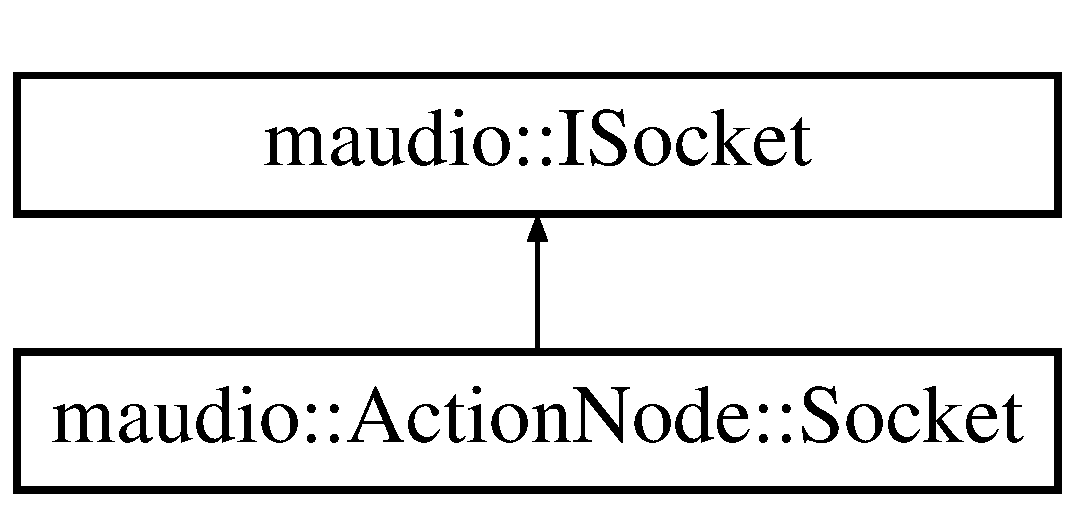
\includegraphics[height=2.000000cm]{classmaudio_1_1ISocket}
\end{center}
\end{figure}
\subsection*{Public Member Functions}
\begin{DoxyCompactItemize}
\item 
virtual \hyperlink{classmaudio_1_1ISocket_a455056af6aaddbea92f1bf6d5cdfc658}{$\sim$\-I\-Socket} ()
\item 
virtual \hyperlink{classmaudio_1_1IAudioBuffer}{I\-Audio\-Buffer} $\ast$ \hyperlink{classmaudio_1_1ISocket_a6a2d1f172963b079563c015ae7338db1}{get} (unsigned long pos, unsigned int length) noexcept=0
\item 
virtual \hyperlink{classmaudio_1_1IAudioInfo}{I\-Audio\-Info} $\ast$ \hyperlink{classmaudio_1_1ISocket_a43b1b9ab16b93131ba7d11204cbe5558}{get\-Info} () noexcept=0
\item 
virtual void \hyperlink{classmaudio_1_1ISocket_a8015c32967e28f35c6abdbe979e4f318}{delete\-Buffer} (\hyperlink{classmaudio_1_1IAudioBuffer}{I\-Audio\-Buffer} $\ast$data) noexcept=0
\item 
virtual void \hyperlink{classmaudio_1_1ISocket_a180a1cb55da56375612a5bdc53be61ee}{delete\-Info} (\hyperlink{classmaudio_1_1IAudioInfo}{I\-Audio\-Info} $\ast$data) noexcept=0
\item 
virtual void \hyperlink{classmaudio_1_1ISocket_ae67025d3d0befc48cbfd11bd05da1386}{delete\-Sample} (\hyperlink{classmaudio_1_1ISample}{I\-Sample} $\ast$data) noexcept=0
\end{DoxyCompactItemize}


\subsection{Constructor \& Destructor Documentation}
\hypertarget{classmaudio_1_1ISocket_a455056af6aaddbea92f1bf6d5cdfc658}{\index{maudio\-::\-I\-Socket@{maudio\-::\-I\-Socket}!$\sim$\-I\-Socket@{$\sim$\-I\-Socket}}
\index{$\sim$\-I\-Socket@{$\sim$\-I\-Socket}!maudio::ISocket@{maudio\-::\-I\-Socket}}
\subsubsection[{$\sim$\-I\-Socket}]{\setlength{\rightskip}{0pt plus 5cm}virtual maudio\-::\-I\-Socket\-::$\sim$\-I\-Socket (
\begin{DoxyParamCaption}
{}
\end{DoxyParamCaption}
)\hspace{0.3cm}{\ttfamily [inline]}, {\ttfamily [virtual]}}}\label{classmaudio_1_1ISocket_a455056af6aaddbea92f1bf6d5cdfc658}


\subsection{Member Function Documentation}
\hypertarget{classmaudio_1_1ISocket_a8015c32967e28f35c6abdbe979e4f318}{\index{maudio\-::\-I\-Socket@{maudio\-::\-I\-Socket}!delete\-Buffer@{delete\-Buffer}}
\index{delete\-Buffer@{delete\-Buffer}!maudio::ISocket@{maudio\-::\-I\-Socket}}
\subsubsection[{delete\-Buffer}]{\setlength{\rightskip}{0pt plus 5cm}virtual void maudio\-::\-I\-Socket\-::delete\-Buffer (
\begin{DoxyParamCaption}
\item[{{\bf I\-Audio\-Buffer} $\ast$}]{data}
\end{DoxyParamCaption}
)\hspace{0.3cm}{\ttfamily [pure virtual]}, {\ttfamily [noexcept]}}}\label{classmaudio_1_1ISocket_a8015c32967e28f35c6abdbe979e4f318}


Implemented in \hyperlink{classmaudio_1_1ActionNode_1_1Socket_a8a64ba64966caca18a70c711ff1e4b2d}{maudio\-::\-Action\-Node\-::\-Socket}.

\hypertarget{classmaudio_1_1ISocket_a180a1cb55da56375612a5bdc53be61ee}{\index{maudio\-::\-I\-Socket@{maudio\-::\-I\-Socket}!delete\-Info@{delete\-Info}}
\index{delete\-Info@{delete\-Info}!maudio::ISocket@{maudio\-::\-I\-Socket}}
\subsubsection[{delete\-Info}]{\setlength{\rightskip}{0pt plus 5cm}virtual void maudio\-::\-I\-Socket\-::delete\-Info (
\begin{DoxyParamCaption}
\item[{{\bf I\-Audio\-Info} $\ast$}]{data}
\end{DoxyParamCaption}
)\hspace{0.3cm}{\ttfamily [pure virtual]}, {\ttfamily [noexcept]}}}\label{classmaudio_1_1ISocket_a180a1cb55da56375612a5bdc53be61ee}


Implemented in \hyperlink{classmaudio_1_1ActionNode_1_1Socket_a3e25c1d6d28ecbfdfeecd6b6c846a1be}{maudio\-::\-Action\-Node\-::\-Socket}.

\hypertarget{classmaudio_1_1ISocket_ae67025d3d0befc48cbfd11bd05da1386}{\index{maudio\-::\-I\-Socket@{maudio\-::\-I\-Socket}!delete\-Sample@{delete\-Sample}}
\index{delete\-Sample@{delete\-Sample}!maudio::ISocket@{maudio\-::\-I\-Socket}}
\subsubsection[{delete\-Sample}]{\setlength{\rightskip}{0pt plus 5cm}virtual void maudio\-::\-I\-Socket\-::delete\-Sample (
\begin{DoxyParamCaption}
\item[{{\bf I\-Sample} $\ast$}]{data}
\end{DoxyParamCaption}
)\hspace{0.3cm}{\ttfamily [pure virtual]}, {\ttfamily [noexcept]}}}\label{classmaudio_1_1ISocket_ae67025d3d0befc48cbfd11bd05da1386}


Implemented in \hyperlink{classmaudio_1_1ActionNode_1_1Socket_a8882eaaf8ea9d06ea006c6d977acdeb7}{maudio\-::\-Action\-Node\-::\-Socket}.

\hypertarget{classmaudio_1_1ISocket_a6a2d1f172963b079563c015ae7338db1}{\index{maudio\-::\-I\-Socket@{maudio\-::\-I\-Socket}!get@{get}}
\index{get@{get}!maudio::ISocket@{maudio\-::\-I\-Socket}}
\subsubsection[{get}]{\setlength{\rightskip}{0pt plus 5cm}virtual {\bf I\-Audio\-Buffer}$\ast$ maudio\-::\-I\-Socket\-::get (
\begin{DoxyParamCaption}
\item[{unsigned long}]{pos, }
\item[{unsigned int}]{length}
\end{DoxyParamCaption}
)\hspace{0.3cm}{\ttfamily [pure virtual]}, {\ttfamily [noexcept]}}}\label{classmaudio_1_1ISocket_a6a2d1f172963b079563c015ae7338db1}


Implemented in \hyperlink{classmaudio_1_1ActionNode_1_1Socket_a3801dbf1ff87f6f4d417d2929ff3c107}{maudio\-::\-Action\-Node\-::\-Socket}.

\hypertarget{classmaudio_1_1ISocket_a43b1b9ab16b93131ba7d11204cbe5558}{\index{maudio\-::\-I\-Socket@{maudio\-::\-I\-Socket}!get\-Info@{get\-Info}}
\index{get\-Info@{get\-Info}!maudio::ISocket@{maudio\-::\-I\-Socket}}
\subsubsection[{get\-Info}]{\setlength{\rightskip}{0pt plus 5cm}virtual {\bf I\-Audio\-Info}$\ast$ maudio\-::\-I\-Socket\-::get\-Info (
\begin{DoxyParamCaption}
{}
\end{DoxyParamCaption}
)\hspace{0.3cm}{\ttfamily [pure virtual]}, {\ttfamily [noexcept]}}}\label{classmaudio_1_1ISocket_a43b1b9ab16b93131ba7d11204cbe5558}


Implemented in \hyperlink{classmaudio_1_1ActionNode_1_1Socket_adf54bb1504b5cf9d53fe6529e86e3653}{maudio\-::\-Action\-Node\-::\-Socket}.



The documentation for this class was generated from the following file\-:\begin{DoxyCompactItemize}
\item 
/home/mars/\-Projekte/maudio/src/plugins/include/core/node/\hyperlink{ISocket_8hpp}{I\-Socket.\-hpp}\end{DoxyCompactItemize}

\hypertarget{classmaudio_1_1KeyValueStore}{\section{maudio\-:\-:Key\-Value\-Store Class Reference}
\label{classmaudio_1_1KeyValueStore}\index{maudio\-::\-Key\-Value\-Store@{maudio\-::\-Key\-Value\-Store}}
}


{\ttfamily \#include $<$Key\-Value\-Store.\-hpp$>$}

Inheritance diagram for maudio\-:\-:Key\-Value\-Store\-:\begin{figure}[H]
\begin{center}
\leavevmode
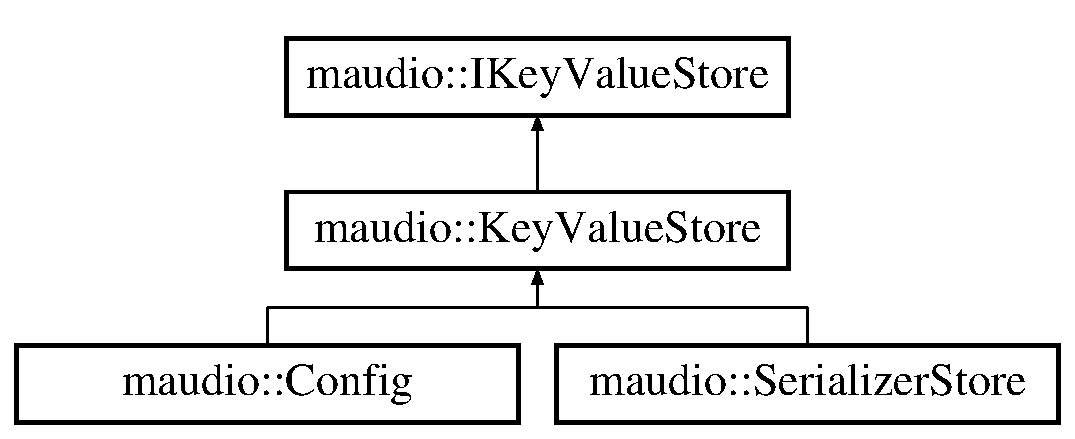
\includegraphics[height=3.000000cm]{classmaudio_1_1KeyValueStore}
\end{center}
\end{figure}
\subsection*{Public Member Functions}
\begin{DoxyCompactItemize}
\item 
\hyperlink{classmaudio_1_1KeyValueStore_a911ecf87816cdd00069de47a65b278c0}{Key\-Value\-Store} ()
\item 
virtual \hyperlink{classmaudio_1_1KeyValueStore_a3f5df2ca00a9e508398aa4fb3ac6498c}{$\sim$\-Key\-Value\-Store} ()
\item 
virtual const char $\ast$ \hyperlink{classmaudio_1_1KeyValueStore_a21db38aeef23adde09a22eea9e85ab71}{get} (const char $\ast$key) const 
\item 
std\-::string \hyperlink{classmaudio_1_1KeyValueStore_aac44d807fbcbbda2b2b555f673e3ed7f}{get} (const std\-::string \&key) const 
\item 
{\footnotesize template$<$typename T $>$ }\\T \hyperlink{classmaudio_1_1KeyValueStore_a4541b1c74b932532f450044e1a417ebd}{get} (const std\-::string \&key) const 
\item 
virtual const char $\ast$ \hyperlink{classmaudio_1_1KeyValueStore_a0c19dbb4603a13e45d4c6a8c8b085758}{get} (unsigned int num\-Key) const 
\item 
{\footnotesize template$<$typename T $>$ }\\T \hyperlink{classmaudio_1_1KeyValueStore_aaafd70f76ca552d5c221414cfb5f49cc}{get} (unsigned int num\-Key) const 
\item 
unsigned int \hyperlink{classmaudio_1_1KeyValueStore_acb51935ff31c59168f72be8af784433a}{get\-Size} () const 
\item 
virtual void \hyperlink{classmaudio_1_1KeyValueStore_a85374af3b968a7bfe7e3e11a9a228375}{set} (const char $\ast$key, const char $\ast$value)
\item 
void \hyperlink{classmaudio_1_1KeyValueStore_a8103b4641569199ed0c6c52796c48354}{set} (const std\-::string \&key, const std\-::string \&value)
\item 
{\footnotesize template$<$typename T $>$ }\\void \hyperlink{classmaudio_1_1KeyValueStore_a8ec3ac184592273483aba5d601613a90}{set} (const std\-::string \&key, T value)
\item 
{\footnotesize template$<$$>$ }\\std\-::string \hyperlink{classmaudio_1_1KeyValueStore_a30cac1374ed8dd15ed1d7398078002e0}{get} (const std\-::string \&key) const 
\item 
{\footnotesize template$<$$>$ }\\std\-::string \hyperlink{classmaudio_1_1KeyValueStore_a5c9e0d1599466bd7895d87a587e1d909}{get} (unsigned int num\-Key) const 
\item 
{\footnotesize template$<$$>$ }\\void \hyperlink{classmaudio_1_1KeyValueStore_a95fbeceb2aa43a23c7aead64a5d74a2d}{set} (const std\-::string \&key, std\-::string value)
\end{DoxyCompactItemize}
\subsection*{Protected Member Functions}
\begin{DoxyCompactItemize}
\item 
bool \hyperlink{classmaudio_1_1KeyValueStore_a9aeb014af614485a7f0627be1c01963c}{check\-Key} (const std\-::string \&key) const 
\end{DoxyCompactItemize}
\subsection*{Protected Attributes}
\begin{DoxyCompactItemize}
\item 
std\-::unordered\-\_\-map\\*
$<$ std\-::string, std\-::string $>$ \hyperlink{classmaudio_1_1KeyValueStore_a024a720cf439988af3e689458bae9bb0}{m\-Data}
\end{DoxyCompactItemize}


\subsection{Constructor \& Destructor Documentation}
\hypertarget{classmaudio_1_1KeyValueStore_a911ecf87816cdd00069de47a65b278c0}{\index{maudio\-::\-Key\-Value\-Store@{maudio\-::\-Key\-Value\-Store}!Key\-Value\-Store@{Key\-Value\-Store}}
\index{Key\-Value\-Store@{Key\-Value\-Store}!maudio::KeyValueStore@{maudio\-::\-Key\-Value\-Store}}
\subsubsection[{Key\-Value\-Store}]{\setlength{\rightskip}{0pt plus 5cm}maudio\-::\-Key\-Value\-Store\-::\-Key\-Value\-Store (
\begin{DoxyParamCaption}
{}
\end{DoxyParamCaption}
)}}\label{classmaudio_1_1KeyValueStore_a911ecf87816cdd00069de47a65b278c0}
\hypertarget{classmaudio_1_1KeyValueStore_a3f5df2ca00a9e508398aa4fb3ac6498c}{\index{maudio\-::\-Key\-Value\-Store@{maudio\-::\-Key\-Value\-Store}!$\sim$\-Key\-Value\-Store@{$\sim$\-Key\-Value\-Store}}
\index{$\sim$\-Key\-Value\-Store@{$\sim$\-Key\-Value\-Store}!maudio::KeyValueStore@{maudio\-::\-Key\-Value\-Store}}
\subsubsection[{$\sim$\-Key\-Value\-Store}]{\setlength{\rightskip}{0pt plus 5cm}maudio\-::\-Key\-Value\-Store\-::$\sim$\-Key\-Value\-Store (
\begin{DoxyParamCaption}
{}
\end{DoxyParamCaption}
)\hspace{0.3cm}{\ttfamily [virtual]}}}\label{classmaudio_1_1KeyValueStore_a3f5df2ca00a9e508398aa4fb3ac6498c}


\subsection{Member Function Documentation}
\hypertarget{classmaudio_1_1KeyValueStore_a9aeb014af614485a7f0627be1c01963c}{\index{maudio\-::\-Key\-Value\-Store@{maudio\-::\-Key\-Value\-Store}!check\-Key@{check\-Key}}
\index{check\-Key@{check\-Key}!maudio::KeyValueStore@{maudio\-::\-Key\-Value\-Store}}
\subsubsection[{check\-Key}]{\setlength{\rightskip}{0pt plus 5cm}bool maudio\-::\-Key\-Value\-Store\-::check\-Key (
\begin{DoxyParamCaption}
\item[{const std\-::string \&}]{key}
\end{DoxyParamCaption}
) const\hspace{0.3cm}{\ttfamily [protected]}}}\label{classmaudio_1_1KeyValueStore_a9aeb014af614485a7f0627be1c01963c}
\hypertarget{classmaudio_1_1KeyValueStore_a21db38aeef23adde09a22eea9e85ab71}{\index{maudio\-::\-Key\-Value\-Store@{maudio\-::\-Key\-Value\-Store}!get@{get}}
\index{get@{get}!maudio::KeyValueStore@{maudio\-::\-Key\-Value\-Store}}
\subsubsection[{get}]{\setlength{\rightskip}{0pt plus 5cm}const char $\ast$ maudio\-::\-Key\-Value\-Store\-::get (
\begin{DoxyParamCaption}
\item[{const char $\ast$}]{key}
\end{DoxyParamCaption}
) const\hspace{0.3cm}{\ttfamily [virtual]}}}\label{classmaudio_1_1KeyValueStore_a21db38aeef23adde09a22eea9e85ab71}


Implements \hyperlink{classmaudio_1_1IKeyValueStore_a3d35bec96b6f1b4301b6ef5e03791181}{maudio\-::\-I\-Key\-Value\-Store}.

\hypertarget{classmaudio_1_1KeyValueStore_aac44d807fbcbbda2b2b555f673e3ed7f}{\index{maudio\-::\-Key\-Value\-Store@{maudio\-::\-Key\-Value\-Store}!get@{get}}
\index{get@{get}!maudio::KeyValueStore@{maudio\-::\-Key\-Value\-Store}}
\subsubsection[{get}]{\setlength{\rightskip}{0pt plus 5cm}std\-::string maudio\-::\-Key\-Value\-Store\-::get (
\begin{DoxyParamCaption}
\item[{const std\-::string \&}]{key}
\end{DoxyParamCaption}
) const}}\label{classmaudio_1_1KeyValueStore_aac44d807fbcbbda2b2b555f673e3ed7f}
\hypertarget{classmaudio_1_1KeyValueStore_a30cac1374ed8dd15ed1d7398078002e0}{\index{maudio\-::\-Key\-Value\-Store@{maudio\-::\-Key\-Value\-Store}!get@{get}}
\index{get@{get}!maudio::KeyValueStore@{maudio\-::\-Key\-Value\-Store}}
\subsubsection[{get}]{\setlength{\rightskip}{0pt plus 5cm}std\-::string maudio\-::\-Key\-Value\-Store\-::get (
\begin{DoxyParamCaption}
\item[{const std\-::string \&}]{key}
\end{DoxyParamCaption}
) const}}\label{classmaudio_1_1KeyValueStore_a30cac1374ed8dd15ed1d7398078002e0}
\hypertarget{classmaudio_1_1KeyValueStore_a4541b1c74b932532f450044e1a417ebd}{\index{maudio\-::\-Key\-Value\-Store@{maudio\-::\-Key\-Value\-Store}!get@{get}}
\index{get@{get}!maudio::KeyValueStore@{maudio\-::\-Key\-Value\-Store}}
\subsubsection[{get}]{\setlength{\rightskip}{0pt plus 5cm}template$<$typename T $>$ T maudio\-::\-Key\-Value\-Store\-::get (
\begin{DoxyParamCaption}
\item[{const std\-::string \&}]{key}
\end{DoxyParamCaption}
) const}}\label{classmaudio_1_1KeyValueStore_a4541b1c74b932532f450044e1a417ebd}
\hypertarget{classmaudio_1_1KeyValueStore_a0c19dbb4603a13e45d4c6a8c8b085758}{\index{maudio\-::\-Key\-Value\-Store@{maudio\-::\-Key\-Value\-Store}!get@{get}}
\index{get@{get}!maudio::KeyValueStore@{maudio\-::\-Key\-Value\-Store}}
\subsubsection[{get}]{\setlength{\rightskip}{0pt plus 5cm}const char $\ast$ maudio\-::\-Key\-Value\-Store\-::get (
\begin{DoxyParamCaption}
\item[{unsigned int}]{num\-Key}
\end{DoxyParamCaption}
) const\hspace{0.3cm}{\ttfamily [virtual]}}}\label{classmaudio_1_1KeyValueStore_a0c19dbb4603a13e45d4c6a8c8b085758}


Implements \hyperlink{classmaudio_1_1IKeyValueStore_a06a7802cc710b2a30dabeabf65326d40}{maudio\-::\-I\-Key\-Value\-Store}.

\hypertarget{classmaudio_1_1KeyValueStore_aaafd70f76ca552d5c221414cfb5f49cc}{\index{maudio\-::\-Key\-Value\-Store@{maudio\-::\-Key\-Value\-Store}!get@{get}}
\index{get@{get}!maudio::KeyValueStore@{maudio\-::\-Key\-Value\-Store}}
\subsubsection[{get}]{\setlength{\rightskip}{0pt plus 5cm}template$<$typename T $>$ T maudio\-::\-Key\-Value\-Store\-::get (
\begin{DoxyParamCaption}
\item[{unsigned int}]{num\-Key}
\end{DoxyParamCaption}
) const\hspace{0.3cm}{\ttfamily [virtual]}}}\label{classmaudio_1_1KeyValueStore_aaafd70f76ca552d5c221414cfb5f49cc}


Implements \hyperlink{classmaudio_1_1IKeyValueStore_a06a7802cc710b2a30dabeabf65326d40}{maudio\-::\-I\-Key\-Value\-Store}.

\hypertarget{classmaudio_1_1KeyValueStore_a5c9e0d1599466bd7895d87a587e1d909}{\index{maudio\-::\-Key\-Value\-Store@{maudio\-::\-Key\-Value\-Store}!get@{get}}
\index{get@{get}!maudio::KeyValueStore@{maudio\-::\-Key\-Value\-Store}}
\subsubsection[{get}]{\setlength{\rightskip}{0pt plus 5cm}std\-::string maudio\-::\-Key\-Value\-Store\-::get (
\begin{DoxyParamCaption}
\item[{unsigned int}]{num\-Key}
\end{DoxyParamCaption}
) const\hspace{0.3cm}{\ttfamily [virtual]}}}\label{classmaudio_1_1KeyValueStore_a5c9e0d1599466bd7895d87a587e1d909}


Implements \hyperlink{classmaudio_1_1IKeyValueStore_a06a7802cc710b2a30dabeabf65326d40}{maudio\-::\-I\-Key\-Value\-Store}.

\hypertarget{classmaudio_1_1KeyValueStore_acb51935ff31c59168f72be8af784433a}{\index{maudio\-::\-Key\-Value\-Store@{maudio\-::\-Key\-Value\-Store}!get\-Size@{get\-Size}}
\index{get\-Size@{get\-Size}!maudio::KeyValueStore@{maudio\-::\-Key\-Value\-Store}}
\subsubsection[{get\-Size}]{\setlength{\rightskip}{0pt plus 5cm}unsigned int maudio\-::\-Key\-Value\-Store\-::get\-Size (
\begin{DoxyParamCaption}
{}
\end{DoxyParamCaption}
) const\hspace{0.3cm}{\ttfamily [virtual]}}}\label{classmaudio_1_1KeyValueStore_acb51935ff31c59168f72be8af784433a}


Implements \hyperlink{classmaudio_1_1IKeyValueStore_ac90d725769db3a9b56803e455dc086c4}{maudio\-::\-I\-Key\-Value\-Store}.

\hypertarget{classmaudio_1_1KeyValueStore_a85374af3b968a7bfe7e3e11a9a228375}{\index{maudio\-::\-Key\-Value\-Store@{maudio\-::\-Key\-Value\-Store}!set@{set}}
\index{set@{set}!maudio::KeyValueStore@{maudio\-::\-Key\-Value\-Store}}
\subsubsection[{set}]{\setlength{\rightskip}{0pt plus 5cm}void maudio\-::\-Key\-Value\-Store\-::set (
\begin{DoxyParamCaption}
\item[{const char $\ast$}]{key, }
\item[{const char $\ast$}]{value}
\end{DoxyParamCaption}
)\hspace{0.3cm}{\ttfamily [virtual]}}}\label{classmaudio_1_1KeyValueStore_a85374af3b968a7bfe7e3e11a9a228375}


Implements \hyperlink{classmaudio_1_1IKeyValueStore_a6baf8502bc2d064d082eabe2072079de}{maudio\-::\-I\-Key\-Value\-Store}.

\hypertarget{classmaudio_1_1KeyValueStore_a8103b4641569199ed0c6c52796c48354}{\index{maudio\-::\-Key\-Value\-Store@{maudio\-::\-Key\-Value\-Store}!set@{set}}
\index{set@{set}!maudio::KeyValueStore@{maudio\-::\-Key\-Value\-Store}}
\subsubsection[{set}]{\setlength{\rightskip}{0pt plus 5cm}void maudio\-::\-Key\-Value\-Store\-::set (
\begin{DoxyParamCaption}
\item[{const std\-::string \&}]{key, }
\item[{const std\-::string \&}]{value}
\end{DoxyParamCaption}
)}}\label{classmaudio_1_1KeyValueStore_a8103b4641569199ed0c6c52796c48354}
\hypertarget{classmaudio_1_1KeyValueStore_a8ec3ac184592273483aba5d601613a90}{\index{maudio\-::\-Key\-Value\-Store@{maudio\-::\-Key\-Value\-Store}!set@{set}}
\index{set@{set}!maudio::KeyValueStore@{maudio\-::\-Key\-Value\-Store}}
\subsubsection[{set}]{\setlength{\rightskip}{0pt plus 5cm}template$<$typename T $>$ void maudio\-::\-Key\-Value\-Store\-::set (
\begin{DoxyParamCaption}
\item[{const std\-::string \&}]{key, }
\item[{T}]{value}
\end{DoxyParamCaption}
)}}\label{classmaudio_1_1KeyValueStore_a8ec3ac184592273483aba5d601613a90}
\hypertarget{classmaudio_1_1KeyValueStore_a95fbeceb2aa43a23c7aead64a5d74a2d}{\index{maudio\-::\-Key\-Value\-Store@{maudio\-::\-Key\-Value\-Store}!set@{set}}
\index{set@{set}!maudio::KeyValueStore@{maudio\-::\-Key\-Value\-Store}}
\subsubsection[{set}]{\setlength{\rightskip}{0pt plus 5cm}void maudio\-::\-Key\-Value\-Store\-::set (
\begin{DoxyParamCaption}
\item[{const std\-::string \&}]{key, }
\item[{std\-::string}]{value}
\end{DoxyParamCaption}
)}}\label{classmaudio_1_1KeyValueStore_a95fbeceb2aa43a23c7aead64a5d74a2d}


\subsection{Member Data Documentation}
\hypertarget{classmaudio_1_1KeyValueStore_a024a720cf439988af3e689458bae9bb0}{\index{maudio\-::\-Key\-Value\-Store@{maudio\-::\-Key\-Value\-Store}!m\-Data@{m\-Data}}
\index{m\-Data@{m\-Data}!maudio::KeyValueStore@{maudio\-::\-Key\-Value\-Store}}
\subsubsection[{m\-Data}]{\setlength{\rightskip}{0pt plus 5cm}std\-::unordered\-\_\-map$<$std\-::string, std\-::string$>$ maudio\-::\-Key\-Value\-Store\-::m\-Data\hspace{0.3cm}{\ttfamily [protected]}}}\label{classmaudio_1_1KeyValueStore_a024a720cf439988af3e689458bae9bb0}


The documentation for this class was generated from the following files\-:\begin{DoxyCompactItemize}
\item 
/home/mars/\-Projekte/maudio/src/plugins/include/core/store/\hyperlink{KeyValueStore_8hpp}{Key\-Value\-Store.\-hpp}\item 
/home/mars/\-Projekte/maudio/src/core/store/\hyperlink{core_2store_2KeyValueStore_8cpp}{Key\-Value\-Store.\-cpp}\end{DoxyCompactItemize}

\hypertarget{classmaudio_1_1MaudioException}{\section{maudio\-:\-:Maudio\-Exception Class Reference}
\label{classmaudio_1_1MaudioException}\index{maudio\-::\-Maudio\-Exception@{maudio\-::\-Maudio\-Exception}}
}


{\ttfamily \#include $<$Audio\-Exception.\-hpp$>$}

Inheritance diagram for maudio\-:\-:Maudio\-Exception\-:\begin{figure}[H]
\begin{center}
\leavevmode
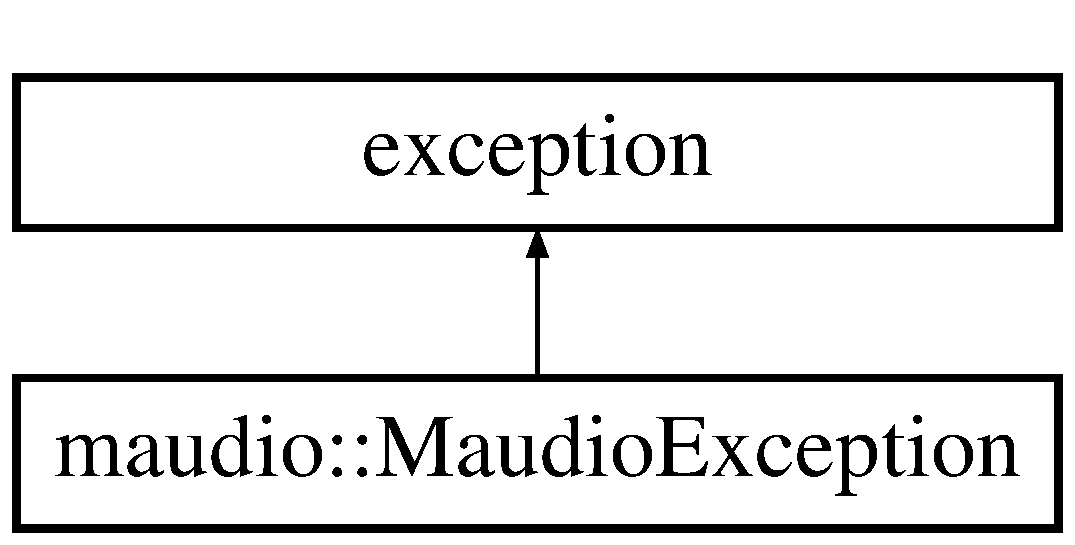
\includegraphics[height=2.000000cm]{classmaudio_1_1MaudioException}
\end{center}
\end{figure}
\subsection*{Public Member Functions}
\begin{DoxyCompactItemize}
\item 
\hyperlink{classmaudio_1_1MaudioException_a649972ea7610ff77dff19bb488b56069}{Maudio\-Exception} (std\-::string \&info)
\item 
\hyperlink{classmaudio_1_1MaudioException_a10d040493ff272ae625ab42876df6515}{Maudio\-Exception} (const char $\ast$info)
\item 
virtual const char $\ast$ \hyperlink{classmaudio_1_1MaudioException_a50ceb3db2d26444b3daa686c4594ca22}{what} () const   throw ()
\end{DoxyCompactItemize}


\subsection{Constructor \& Destructor Documentation}
\hypertarget{classmaudio_1_1MaudioException_a649972ea7610ff77dff19bb488b56069}{\index{maudio\-::\-Maudio\-Exception@{maudio\-::\-Maudio\-Exception}!Maudio\-Exception@{Maudio\-Exception}}
\index{Maudio\-Exception@{Maudio\-Exception}!maudio::MaudioException@{maudio\-::\-Maudio\-Exception}}
\subsubsection[{Maudio\-Exception}]{\setlength{\rightskip}{0pt plus 5cm}maudio\-::\-Maudio\-Exception\-::\-Maudio\-Exception (
\begin{DoxyParamCaption}
\item[{std\-::string \&}]{info}
\end{DoxyParamCaption}
)\hspace{0.3cm}{\ttfamily [inline]}}}\label{classmaudio_1_1MaudioException_a649972ea7610ff77dff19bb488b56069}
\hypertarget{classmaudio_1_1MaudioException_a10d040493ff272ae625ab42876df6515}{\index{maudio\-::\-Maudio\-Exception@{maudio\-::\-Maudio\-Exception}!Maudio\-Exception@{Maudio\-Exception}}
\index{Maudio\-Exception@{Maudio\-Exception}!maudio::MaudioException@{maudio\-::\-Maudio\-Exception}}
\subsubsection[{Maudio\-Exception}]{\setlength{\rightskip}{0pt plus 5cm}maudio\-::\-Maudio\-Exception\-::\-Maudio\-Exception (
\begin{DoxyParamCaption}
\item[{const char $\ast$}]{info}
\end{DoxyParamCaption}
)\hspace{0.3cm}{\ttfamily [inline]}}}\label{classmaudio_1_1MaudioException_a10d040493ff272ae625ab42876df6515}


\subsection{Member Function Documentation}
\hypertarget{classmaudio_1_1MaudioException_a50ceb3db2d26444b3daa686c4594ca22}{\index{maudio\-::\-Maudio\-Exception@{maudio\-::\-Maudio\-Exception}!what@{what}}
\index{what@{what}!maudio::MaudioException@{maudio\-::\-Maudio\-Exception}}
\subsubsection[{what}]{\setlength{\rightskip}{0pt plus 5cm}virtual const char$\ast$ maudio\-::\-Maudio\-Exception\-::what (
\begin{DoxyParamCaption}
{}
\end{DoxyParamCaption}
) const throw  ) \hspace{0.3cm}{\ttfamily [inline]}, {\ttfamily [virtual]}}}\label{classmaudio_1_1MaudioException_a50ceb3db2d26444b3daa686c4594ca22}


The documentation for this class was generated from the following file\-:\begin{DoxyCompactItemize}
\item 
/home/mars/\-Projekte/maudio/src/plugins/include/core/util/\hyperlink{AudioException_8hpp}{Audio\-Exception.\-hpp}\end{DoxyCompactItemize}

\hypertarget{classmaudio_1_1Node}{\section{maudio\-:\-:Node Class Reference}
\label{classmaudio_1_1Node}\index{maudio\-::\-Node@{maudio\-::\-Node}}
}


{\ttfamily \#include $<$Node.\-hpp$>$}

Inheritance diagram for maudio\-:\-:Node\-:\begin{figure}[H]
\begin{center}
\leavevmode
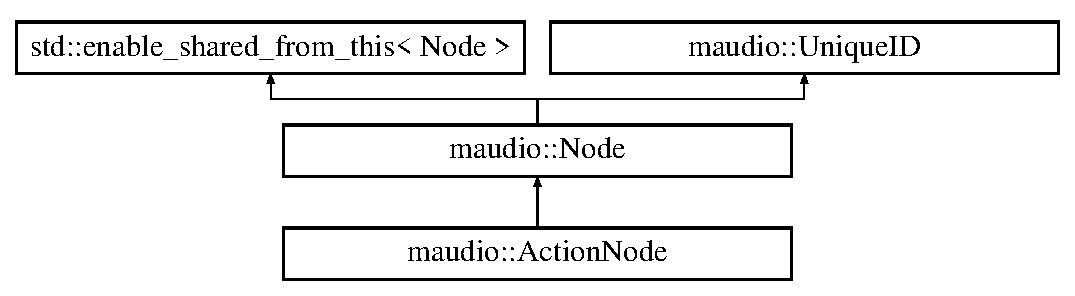
\includegraphics[height=3.000000cm]{classmaudio_1_1Node}
\end{center}
\end{figure}
\subsection*{Public Member Functions}
\begin{DoxyCompactItemize}
\item 
virtual \hyperlink{classmaudio_1_1Node_aac4476ebe448f6a52e43b049484c3758}{$\sim$\-Node} ()
\item 
virtual \hyperlink{classmaudio_1_1IAudioBuffer}{I\-Audio\-Buffer} $\ast$ \hyperlink{classmaudio_1_1Node_a19514a2d372ace1179e2b910b13ee26c}{get} (unsigned long pos, unsigned int length) noexcept=0
\item 
virtual \hyperlink{classmaudio_1_1IAudioInfo}{I\-Audio\-Info} $\ast$ \hyperlink{classmaudio_1_1Node_a7e8a3c69d7d49328dba7f0ab004a6bd4}{get\-Info} () noexcept=0
\item 
virtual void \hyperlink{classmaudio_1_1Node_a11f8c628cc1d1994ad45e9ea81d5e27c}{delete\-Buffer} (\hyperlink{classmaudio_1_1IAudioBuffer}{I\-Audio\-Buffer} $\ast$data) noexcept=0
\item 
virtual void \hyperlink{classmaudio_1_1Node_af9a851c3aa51799a416f4a42acb15617}{delete\-Info} (\hyperlink{classmaudio_1_1IAudioInfo}{I\-Audio\-Info} $\ast$data) noexcept=0
\item 
virtual void \hyperlink{classmaudio_1_1Node_a4a6a5d0dc79d3bee44d3284517bdfe2b}{delete\-Sample} (\hyperlink{classmaudio_1_1ISample}{I\-Sample} $\ast$data) noexcept=0
\item 
void \hyperlink{classmaudio_1_1Node_aa989f49d7ee91c9b6889a2f75e443273}{add\-Input} (std\-::shared\-\_\-ptr$<$ \hyperlink{classmaudio_1_1Node}{Node} $>$ node, int slot=-\/1)
\item 
void \hyperlink{classmaudio_1_1Node_aafffc41b14d93b275c4945966a032cba}{remove\-Input} (std\-::shared\-\_\-ptr$<$ \hyperlink{classmaudio_1_1Node}{Node} $>$ node)
\item 
void \hyperlink{classmaudio_1_1Node_abcf1492e0e46096af20040081c9e4b45}{remove\-Input} (int slot)
\item 
std\-::shared\-\_\-ptr$<$ \hyperlink{classmaudio_1_1Node}{Node} $>$ \hyperlink{classmaudio_1_1Node_a9dd19525ec456748a58bfd13be6de386}{get\-Input} (int slot)
\item 
std\-::shared\-\_\-ptr$<$ \hyperlink{classmaudio_1_1Node}{Node} $>$ \hyperlink{classmaudio_1_1Node_abdf6a8a71127b38d8f8a2f5bd3fda3d3}{get\-Output} (int slot)
\item 
std\-::shared\-\_\-ptr$<$ \hyperlink{classmaudio_1_1Node}{Node} $>$ \hyperlink{classmaudio_1_1Node_a63bc55e437f828250b4bdd86862d3da1}{get\-By\-I\-D} (unsigned int id)
\item 
void \hyperlink{classmaudio_1_1Node_ab26d293b4a4da29bae7c2303d37ea9ad}{disconnect} ()
\item 
virtual unsigned int \hyperlink{classmaudio_1_1Node_aa388047f9fd7356e1555d481ce39284e}{Num\-Inputs} () const 
\item 
virtual unsigned int \hyperlink{classmaudio_1_1Node_a1a8c27fc95cf959d243a76351383071d}{Num\-Outputs} () const 
\item 
virtual int \hyperlink{classmaudio_1_1Node_a2d3df13430b6ee1ba1a08a2bfc04d092}{Max\-Inputs} () const =0
\item 
virtual bool \hyperlink{classmaudio_1_1Node_adefc8b35c3242b11730071d72dd8cf83}{Has\-Outputs} () const =0
\item 
virtual void \hyperlink{classmaudio_1_1Node_aab5537a1cda3ec0db8c7a91545066197}{read\-Config} (const \hyperlink{classmaudio_1_1Config}{Config} \&conf)=0
\item 
virtual \hyperlink{classmaudio_1_1IPropertyManager}{I\-Property\-Manager} $\ast$ \hyperlink{classmaudio_1_1Node_ac9960215fa9c0201f1fc31f4f206036c}{get\-Properties} ()=0
\item 
virtual \hyperlink{classmaudio_1_1IControl}{I\-Control} $\ast$ \hyperlink{classmaudio_1_1Node_a4cf6cb717e8811c64bc018bae9248b9f}{get\-Control} ()=0
\item 
std\-::string \hyperlink{classmaudio_1_1Node_acb00c66166f4c0b409e18b1014bcf2e5}{get\-Name} () const 
\item 
void \hyperlink{classmaudio_1_1Node_a63c854dc748dd1f7bafa51f502699774}{set\-Name} (const std\-::string \&name)
\item 
virtual \hyperlink{classmaudio_1_1IKeyValueStore}{I\-Key\-Value\-Store} $\ast$ \hyperlink{classmaudio_1_1Node_a264737e69763b0aa28277c52a772a14f}{serialize} () const =0
\item 
virtual void \hyperlink{classmaudio_1_1Node_af6be2a9f71d265bdbd5a230a58c8138c}{deserialize} (const \hyperlink{classmaudio_1_1IKeyValueStore}{I\-Key\-Value\-Store} $\ast$data)=0
\end{DoxyCompactItemize}
\subsection*{Protected Member Functions}
\begin{DoxyCompactItemize}
\item 
virtual void \hyperlink{classmaudio_1_1Node_aef1bcd3c5642c86495259b638ab54290}{on\-Add} (unsigned int slot)=0
\item 
virtual void \hyperlink{classmaudio_1_1Node_a058346c2dddf4e1cb061fadbd433446e}{on\-Remove} (unsigned int slot)=0
\end{DoxyCompactItemize}
\subsection*{Protected Attributes}
\begin{DoxyCompactItemize}
\item 
std\-::vector$<$ std\-::shared\-\_\-ptr\\*
$<$ \hyperlink{classmaudio_1_1Node}{Node} $>$ $>$ \hyperlink{classmaudio_1_1Node_affc36c6e75daffd04ef638cab22d84a0}{m\-Inputs}
\item 
std\-::vector$<$ std\-::weak\-\_\-ptr\\*
$<$ \hyperlink{classmaudio_1_1Node}{Node} $>$ $>$ \hyperlink{classmaudio_1_1Node_a75658f4f37faf14b438a95b7d8d60048}{m\-Outputs}
\end{DoxyCompactItemize}


\subsection{Constructor \& Destructor Documentation}
\hypertarget{classmaudio_1_1Node_aac4476ebe448f6a52e43b049484c3758}{\index{maudio\-::\-Node@{maudio\-::\-Node}!$\sim$\-Node@{$\sim$\-Node}}
\index{$\sim$\-Node@{$\sim$\-Node}!maudio::Node@{maudio\-::\-Node}}
\subsubsection[{$\sim$\-Node}]{\setlength{\rightskip}{0pt plus 5cm}maudio\-::\-Node\-::$\sim$\-Node (
\begin{DoxyParamCaption}
{}
\end{DoxyParamCaption}
)\hspace{0.3cm}{\ttfamily [virtual]}}}\label{classmaudio_1_1Node_aac4476ebe448f6a52e43b049484c3758}


\subsection{Member Function Documentation}
\hypertarget{classmaudio_1_1Node_aa989f49d7ee91c9b6889a2f75e443273}{\index{maudio\-::\-Node@{maudio\-::\-Node}!add\-Input@{add\-Input}}
\index{add\-Input@{add\-Input}!maudio::Node@{maudio\-::\-Node}}
\subsubsection[{add\-Input}]{\setlength{\rightskip}{0pt plus 5cm}void maudio\-::\-Node\-::add\-Input (
\begin{DoxyParamCaption}
\item[{std\-::shared\-\_\-ptr$<$ {\bf Node} $>$}]{node, }
\item[{int}]{slot = {\ttfamily -\/1}}
\end{DoxyParamCaption}
)}}\label{classmaudio_1_1Node_aa989f49d7ee91c9b6889a2f75e443273}
\hypertarget{classmaudio_1_1Node_a11f8c628cc1d1994ad45e9ea81d5e27c}{\index{maudio\-::\-Node@{maudio\-::\-Node}!delete\-Buffer@{delete\-Buffer}}
\index{delete\-Buffer@{delete\-Buffer}!maudio::Node@{maudio\-::\-Node}}
\subsubsection[{delete\-Buffer}]{\setlength{\rightskip}{0pt plus 5cm}virtual void maudio\-::\-Node\-::delete\-Buffer (
\begin{DoxyParamCaption}
\item[{{\bf I\-Audio\-Buffer} $\ast$}]{data}
\end{DoxyParamCaption}
)\hspace{0.3cm}{\ttfamily [pure virtual]}, {\ttfamily [noexcept]}}}\label{classmaudio_1_1Node_a11f8c628cc1d1994ad45e9ea81d5e27c}


Implemented in \hyperlink{classmaudio_1_1ActionNode_ad89fda4bd963d3176ad61dfd414596a5}{maudio\-::\-Action\-Node}.

\hypertarget{classmaudio_1_1Node_af9a851c3aa51799a416f4a42acb15617}{\index{maudio\-::\-Node@{maudio\-::\-Node}!delete\-Info@{delete\-Info}}
\index{delete\-Info@{delete\-Info}!maudio::Node@{maudio\-::\-Node}}
\subsubsection[{delete\-Info}]{\setlength{\rightskip}{0pt plus 5cm}virtual void maudio\-::\-Node\-::delete\-Info (
\begin{DoxyParamCaption}
\item[{{\bf I\-Audio\-Info} $\ast$}]{data}
\end{DoxyParamCaption}
)\hspace{0.3cm}{\ttfamily [pure virtual]}, {\ttfamily [noexcept]}}}\label{classmaudio_1_1Node_af9a851c3aa51799a416f4a42acb15617}


Implemented in \hyperlink{classmaudio_1_1ActionNode_a2cedf925663e0c898fae99e826586e9a}{maudio\-::\-Action\-Node}.

\hypertarget{classmaudio_1_1Node_a4a6a5d0dc79d3bee44d3284517bdfe2b}{\index{maudio\-::\-Node@{maudio\-::\-Node}!delete\-Sample@{delete\-Sample}}
\index{delete\-Sample@{delete\-Sample}!maudio::Node@{maudio\-::\-Node}}
\subsubsection[{delete\-Sample}]{\setlength{\rightskip}{0pt plus 5cm}virtual void maudio\-::\-Node\-::delete\-Sample (
\begin{DoxyParamCaption}
\item[{{\bf I\-Sample} $\ast$}]{data}
\end{DoxyParamCaption}
)\hspace{0.3cm}{\ttfamily [pure virtual]}, {\ttfamily [noexcept]}}}\label{classmaudio_1_1Node_a4a6a5d0dc79d3bee44d3284517bdfe2b}


Implemented in \hyperlink{classmaudio_1_1ActionNode_ac10ce0b12b802fb444c91999337ac3dc}{maudio\-::\-Action\-Node}.

\hypertarget{classmaudio_1_1Node_af6be2a9f71d265bdbd5a230a58c8138c}{\index{maudio\-::\-Node@{maudio\-::\-Node}!deserialize@{deserialize}}
\index{deserialize@{deserialize}!maudio::Node@{maudio\-::\-Node}}
\subsubsection[{deserialize}]{\setlength{\rightskip}{0pt plus 5cm}virtual void maudio\-::\-Node\-::deserialize (
\begin{DoxyParamCaption}
\item[{const {\bf I\-Key\-Value\-Store} $\ast$}]{data}
\end{DoxyParamCaption}
)\hspace{0.3cm}{\ttfamily [pure virtual]}}}\label{classmaudio_1_1Node_af6be2a9f71d265bdbd5a230a58c8138c}


Implemented in \hyperlink{classmaudio_1_1ActionNode_a7e416ec107ebbcb1ed6c771cf35acab5}{maudio\-::\-Action\-Node}.

\hypertarget{classmaudio_1_1Node_ab26d293b4a4da29bae7c2303d37ea9ad}{\index{maudio\-::\-Node@{maudio\-::\-Node}!disconnect@{disconnect}}
\index{disconnect@{disconnect}!maudio::Node@{maudio\-::\-Node}}
\subsubsection[{disconnect}]{\setlength{\rightskip}{0pt plus 5cm}void maudio\-::\-Node\-::disconnect (
\begin{DoxyParamCaption}
{}
\end{DoxyParamCaption}
)}}\label{classmaudio_1_1Node_ab26d293b4a4da29bae7c2303d37ea9ad}
\hypertarget{classmaudio_1_1Node_a19514a2d372ace1179e2b910b13ee26c}{\index{maudio\-::\-Node@{maudio\-::\-Node}!get@{get}}
\index{get@{get}!maudio::Node@{maudio\-::\-Node}}
\subsubsection[{get}]{\setlength{\rightskip}{0pt plus 5cm}virtual {\bf I\-Audio\-Buffer}$\ast$ maudio\-::\-Node\-::get (
\begin{DoxyParamCaption}
\item[{unsigned long}]{pos, }
\item[{unsigned int}]{length}
\end{DoxyParamCaption}
)\hspace{0.3cm}{\ttfamily [pure virtual]}, {\ttfamily [noexcept]}}}\label{classmaudio_1_1Node_a19514a2d372ace1179e2b910b13ee26c}


Implemented in \hyperlink{classmaudio_1_1ActionNode_a7dad30c2c187519dfb8508a088a2d842}{maudio\-::\-Action\-Node}.

\hypertarget{classmaudio_1_1Node_a63bc55e437f828250b4bdd86862d3da1}{\index{maudio\-::\-Node@{maudio\-::\-Node}!get\-By\-I\-D@{get\-By\-I\-D}}
\index{get\-By\-I\-D@{get\-By\-I\-D}!maudio::Node@{maudio\-::\-Node}}
\subsubsection[{get\-By\-I\-D}]{\setlength{\rightskip}{0pt plus 5cm}std\-::shared\-\_\-ptr$<$ {\bf Node} $>$ maudio\-::\-Node\-::get\-By\-I\-D (
\begin{DoxyParamCaption}
\item[{unsigned int}]{id}
\end{DoxyParamCaption}
)}}\label{classmaudio_1_1Node_a63bc55e437f828250b4bdd86862d3da1}
\hypertarget{classmaudio_1_1Node_a4cf6cb717e8811c64bc018bae9248b9f}{\index{maudio\-::\-Node@{maudio\-::\-Node}!get\-Control@{get\-Control}}
\index{get\-Control@{get\-Control}!maudio::Node@{maudio\-::\-Node}}
\subsubsection[{get\-Control}]{\setlength{\rightskip}{0pt plus 5cm}virtual {\bf I\-Control}$\ast$ maudio\-::\-Node\-::get\-Control (
\begin{DoxyParamCaption}
{}
\end{DoxyParamCaption}
)\hspace{0.3cm}{\ttfamily [pure virtual]}}}\label{classmaudio_1_1Node_a4cf6cb717e8811c64bc018bae9248b9f}


Implemented in \hyperlink{classmaudio_1_1ActionNode_aa4647a1e40a0ce5f3b19098ed347b5da}{maudio\-::\-Action\-Node}.

\hypertarget{classmaudio_1_1Node_a7e8a3c69d7d49328dba7f0ab004a6bd4}{\index{maudio\-::\-Node@{maudio\-::\-Node}!get\-Info@{get\-Info}}
\index{get\-Info@{get\-Info}!maudio::Node@{maudio\-::\-Node}}
\subsubsection[{get\-Info}]{\setlength{\rightskip}{0pt plus 5cm}virtual {\bf I\-Audio\-Info}$\ast$ maudio\-::\-Node\-::get\-Info (
\begin{DoxyParamCaption}
{}
\end{DoxyParamCaption}
)\hspace{0.3cm}{\ttfamily [pure virtual]}, {\ttfamily [noexcept]}}}\label{classmaudio_1_1Node_a7e8a3c69d7d49328dba7f0ab004a6bd4}


Implemented in \hyperlink{classmaudio_1_1ActionNode_a10c712ce5741eeeeb46fc8cadf9687b5}{maudio\-::\-Action\-Node}.

\hypertarget{classmaudio_1_1Node_a9dd19525ec456748a58bfd13be6de386}{\index{maudio\-::\-Node@{maudio\-::\-Node}!get\-Input@{get\-Input}}
\index{get\-Input@{get\-Input}!maudio::Node@{maudio\-::\-Node}}
\subsubsection[{get\-Input}]{\setlength{\rightskip}{0pt plus 5cm}std\-::shared\-\_\-ptr$<$ {\bf Node} $>$ maudio\-::\-Node\-::get\-Input (
\begin{DoxyParamCaption}
\item[{int}]{slot}
\end{DoxyParamCaption}
)}}\label{classmaudio_1_1Node_a9dd19525ec456748a58bfd13be6de386}
\hypertarget{classmaudio_1_1Node_acb00c66166f4c0b409e18b1014bcf2e5}{\index{maudio\-::\-Node@{maudio\-::\-Node}!get\-Name@{get\-Name}}
\index{get\-Name@{get\-Name}!maudio::Node@{maudio\-::\-Node}}
\subsubsection[{get\-Name}]{\setlength{\rightskip}{0pt plus 5cm}std\-::string maudio\-::\-Node\-::get\-Name (
\begin{DoxyParamCaption}
{}
\end{DoxyParamCaption}
) const}}\label{classmaudio_1_1Node_acb00c66166f4c0b409e18b1014bcf2e5}
\hypertarget{classmaudio_1_1Node_abdf6a8a71127b38d8f8a2f5bd3fda3d3}{\index{maudio\-::\-Node@{maudio\-::\-Node}!get\-Output@{get\-Output}}
\index{get\-Output@{get\-Output}!maudio::Node@{maudio\-::\-Node}}
\subsubsection[{get\-Output}]{\setlength{\rightskip}{0pt plus 5cm}std\-::shared\-\_\-ptr$<$ {\bf Node} $>$ maudio\-::\-Node\-::get\-Output (
\begin{DoxyParamCaption}
\item[{int}]{slot}
\end{DoxyParamCaption}
)}}\label{classmaudio_1_1Node_abdf6a8a71127b38d8f8a2f5bd3fda3d3}
\hypertarget{classmaudio_1_1Node_ac9960215fa9c0201f1fc31f4f206036c}{\index{maudio\-::\-Node@{maudio\-::\-Node}!get\-Properties@{get\-Properties}}
\index{get\-Properties@{get\-Properties}!maudio::Node@{maudio\-::\-Node}}
\subsubsection[{get\-Properties}]{\setlength{\rightskip}{0pt plus 5cm}virtual {\bf I\-Property\-Manager}$\ast$ maudio\-::\-Node\-::get\-Properties (
\begin{DoxyParamCaption}
{}
\end{DoxyParamCaption}
)\hspace{0.3cm}{\ttfamily [pure virtual]}}}\label{classmaudio_1_1Node_ac9960215fa9c0201f1fc31f4f206036c}


Implemented in \hyperlink{classmaudio_1_1ActionNode_a8f9a10275ff3bf112c7f14e896d14c06}{maudio\-::\-Action\-Node}.

\hypertarget{classmaudio_1_1Node_adefc8b35c3242b11730071d72dd8cf83}{\index{maudio\-::\-Node@{maudio\-::\-Node}!Has\-Outputs@{Has\-Outputs}}
\index{Has\-Outputs@{Has\-Outputs}!maudio::Node@{maudio\-::\-Node}}
\subsubsection[{Has\-Outputs}]{\setlength{\rightskip}{0pt plus 5cm}virtual bool maudio\-::\-Node\-::\-Has\-Outputs (
\begin{DoxyParamCaption}
{}
\end{DoxyParamCaption}
) const\hspace{0.3cm}{\ttfamily [pure virtual]}}}\label{classmaudio_1_1Node_adefc8b35c3242b11730071d72dd8cf83}


Implemented in \hyperlink{classmaudio_1_1ActionNode_a7f43a61f1da08dd12688d5480677b8c1}{maudio\-::\-Action\-Node}.

\hypertarget{classmaudio_1_1Node_a2d3df13430b6ee1ba1a08a2bfc04d092}{\index{maudio\-::\-Node@{maudio\-::\-Node}!Max\-Inputs@{Max\-Inputs}}
\index{Max\-Inputs@{Max\-Inputs}!maudio::Node@{maudio\-::\-Node}}
\subsubsection[{Max\-Inputs}]{\setlength{\rightskip}{0pt plus 5cm}virtual int maudio\-::\-Node\-::\-Max\-Inputs (
\begin{DoxyParamCaption}
{}
\end{DoxyParamCaption}
) const\hspace{0.3cm}{\ttfamily [pure virtual]}}}\label{classmaudio_1_1Node_a2d3df13430b6ee1ba1a08a2bfc04d092}


Implemented in \hyperlink{classmaudio_1_1ActionNode_a6e6e10558f7cc555f1dcbe2de6b5cdb2}{maudio\-::\-Action\-Node}.

\hypertarget{classmaudio_1_1Node_aa388047f9fd7356e1555d481ce39284e}{\index{maudio\-::\-Node@{maudio\-::\-Node}!Num\-Inputs@{Num\-Inputs}}
\index{Num\-Inputs@{Num\-Inputs}!maudio::Node@{maudio\-::\-Node}}
\subsubsection[{Num\-Inputs}]{\setlength{\rightskip}{0pt plus 5cm}unsigned int maudio\-::\-Node\-::\-Num\-Inputs (
\begin{DoxyParamCaption}
{}
\end{DoxyParamCaption}
) const\hspace{0.3cm}{\ttfamily [virtual]}}}\label{classmaudio_1_1Node_aa388047f9fd7356e1555d481ce39284e}
\hypertarget{classmaudio_1_1Node_a1a8c27fc95cf959d243a76351383071d}{\index{maudio\-::\-Node@{maudio\-::\-Node}!Num\-Outputs@{Num\-Outputs}}
\index{Num\-Outputs@{Num\-Outputs}!maudio::Node@{maudio\-::\-Node}}
\subsubsection[{Num\-Outputs}]{\setlength{\rightskip}{0pt plus 5cm}unsigned int maudio\-::\-Node\-::\-Num\-Outputs (
\begin{DoxyParamCaption}
{}
\end{DoxyParamCaption}
) const\hspace{0.3cm}{\ttfamily [virtual]}}}\label{classmaudio_1_1Node_a1a8c27fc95cf959d243a76351383071d}
\hypertarget{classmaudio_1_1Node_aef1bcd3c5642c86495259b638ab54290}{\index{maudio\-::\-Node@{maudio\-::\-Node}!on\-Add@{on\-Add}}
\index{on\-Add@{on\-Add}!maudio::Node@{maudio\-::\-Node}}
\subsubsection[{on\-Add}]{\setlength{\rightskip}{0pt plus 5cm}virtual void maudio\-::\-Node\-::on\-Add (
\begin{DoxyParamCaption}
\item[{unsigned int}]{slot}
\end{DoxyParamCaption}
)\hspace{0.3cm}{\ttfamily [protected]}, {\ttfamily [pure virtual]}}}\label{classmaudio_1_1Node_aef1bcd3c5642c86495259b638ab54290}


Implemented in \hyperlink{classmaudio_1_1ActionNode_ad2a0d41f2370fa8a32fc4e6ce2bb9eef}{maudio\-::\-Action\-Node}.

\hypertarget{classmaudio_1_1Node_a058346c2dddf4e1cb061fadbd433446e}{\index{maudio\-::\-Node@{maudio\-::\-Node}!on\-Remove@{on\-Remove}}
\index{on\-Remove@{on\-Remove}!maudio::Node@{maudio\-::\-Node}}
\subsubsection[{on\-Remove}]{\setlength{\rightskip}{0pt plus 5cm}virtual void maudio\-::\-Node\-::on\-Remove (
\begin{DoxyParamCaption}
\item[{unsigned int}]{slot}
\end{DoxyParamCaption}
)\hspace{0.3cm}{\ttfamily [protected]}, {\ttfamily [pure virtual]}}}\label{classmaudio_1_1Node_a058346c2dddf4e1cb061fadbd433446e}


Implemented in \hyperlink{classmaudio_1_1ActionNode_aaa27a57824ba5e990d935ef117b6ef69}{maudio\-::\-Action\-Node}.

\hypertarget{classmaudio_1_1Node_aab5537a1cda3ec0db8c7a91545066197}{\index{maudio\-::\-Node@{maudio\-::\-Node}!read\-Config@{read\-Config}}
\index{read\-Config@{read\-Config}!maudio::Node@{maudio\-::\-Node}}
\subsubsection[{read\-Config}]{\setlength{\rightskip}{0pt plus 5cm}virtual void maudio\-::\-Node\-::read\-Config (
\begin{DoxyParamCaption}
\item[{const {\bf Config} \&}]{conf}
\end{DoxyParamCaption}
)\hspace{0.3cm}{\ttfamily [pure virtual]}}}\label{classmaudio_1_1Node_aab5537a1cda3ec0db8c7a91545066197}


Implemented in \hyperlink{classmaudio_1_1ActionNode_aba178721f832128b48adc02550545ce1}{maudio\-::\-Action\-Node}.

\hypertarget{classmaudio_1_1Node_aafffc41b14d93b275c4945966a032cba}{\index{maudio\-::\-Node@{maudio\-::\-Node}!remove\-Input@{remove\-Input}}
\index{remove\-Input@{remove\-Input}!maudio::Node@{maudio\-::\-Node}}
\subsubsection[{remove\-Input}]{\setlength{\rightskip}{0pt plus 5cm}void maudio\-::\-Node\-::remove\-Input (
\begin{DoxyParamCaption}
\item[{std\-::shared\-\_\-ptr$<$ {\bf Node} $>$}]{node}
\end{DoxyParamCaption}
)}}\label{classmaudio_1_1Node_aafffc41b14d93b275c4945966a032cba}
\hypertarget{classmaudio_1_1Node_abcf1492e0e46096af20040081c9e4b45}{\index{maudio\-::\-Node@{maudio\-::\-Node}!remove\-Input@{remove\-Input}}
\index{remove\-Input@{remove\-Input}!maudio::Node@{maudio\-::\-Node}}
\subsubsection[{remove\-Input}]{\setlength{\rightskip}{0pt plus 5cm}void maudio\-::\-Node\-::remove\-Input (
\begin{DoxyParamCaption}
\item[{int}]{slot}
\end{DoxyParamCaption}
)}}\label{classmaudio_1_1Node_abcf1492e0e46096af20040081c9e4b45}
\hypertarget{classmaudio_1_1Node_a264737e69763b0aa28277c52a772a14f}{\index{maudio\-::\-Node@{maudio\-::\-Node}!serialize@{serialize}}
\index{serialize@{serialize}!maudio::Node@{maudio\-::\-Node}}
\subsubsection[{serialize}]{\setlength{\rightskip}{0pt plus 5cm}virtual {\bf I\-Key\-Value\-Store}$\ast$ maudio\-::\-Node\-::serialize (
\begin{DoxyParamCaption}
{}
\end{DoxyParamCaption}
) const\hspace{0.3cm}{\ttfamily [pure virtual]}}}\label{classmaudio_1_1Node_a264737e69763b0aa28277c52a772a14f}


Implemented in \hyperlink{classmaudio_1_1ActionNode_a7aa30b6bf8a68cb222472f4e20d05b13}{maudio\-::\-Action\-Node}.

\hypertarget{classmaudio_1_1Node_a63c854dc748dd1f7bafa51f502699774}{\index{maudio\-::\-Node@{maudio\-::\-Node}!set\-Name@{set\-Name}}
\index{set\-Name@{set\-Name}!maudio::Node@{maudio\-::\-Node}}
\subsubsection[{set\-Name}]{\setlength{\rightskip}{0pt plus 5cm}void maudio\-::\-Node\-::set\-Name (
\begin{DoxyParamCaption}
\item[{const std\-::string \&}]{name}
\end{DoxyParamCaption}
)}}\label{classmaudio_1_1Node_a63c854dc748dd1f7bafa51f502699774}


\subsection{Member Data Documentation}
\hypertarget{classmaudio_1_1Node_affc36c6e75daffd04ef638cab22d84a0}{\index{maudio\-::\-Node@{maudio\-::\-Node}!m\-Inputs@{m\-Inputs}}
\index{m\-Inputs@{m\-Inputs}!maudio::Node@{maudio\-::\-Node}}
\subsubsection[{m\-Inputs}]{\setlength{\rightskip}{0pt plus 5cm}std\-::vector$<$std\-::shared\-\_\-ptr$<${\bf Node}$>$ $>$ maudio\-::\-Node\-::m\-Inputs\hspace{0.3cm}{\ttfamily [protected]}}}\label{classmaudio_1_1Node_affc36c6e75daffd04ef638cab22d84a0}
\hypertarget{classmaudio_1_1Node_a75658f4f37faf14b438a95b7d8d60048}{\index{maudio\-::\-Node@{maudio\-::\-Node}!m\-Outputs@{m\-Outputs}}
\index{m\-Outputs@{m\-Outputs}!maudio::Node@{maudio\-::\-Node}}
\subsubsection[{m\-Outputs}]{\setlength{\rightskip}{0pt plus 5cm}std\-::vector$<$std\-::weak\-\_\-ptr$<${\bf Node}$>$ $>$ maudio\-::\-Node\-::m\-Outputs\hspace{0.3cm}{\ttfamily [protected]}}}\label{classmaudio_1_1Node_a75658f4f37faf14b438a95b7d8d60048}


The documentation for this class was generated from the following files\-:\begin{DoxyCompactItemize}
\item 
/home/mars/\-Projekte/maudio/src/plugins/include/core/node/\hyperlink{Node_8hpp}{Node.\-hpp}\item 
/home/mars/\-Projekte/maudio/src/core/node/\hyperlink{core_2node_2Node_8cpp}{Node.\-cpp}\end{DoxyCompactItemize}

\hypertarget{classmaudio_1_1OutOfBoundsException}{\section{maudio\-:\-:Out\-Of\-Bounds\-Exception Class Reference}
\label{classmaudio_1_1OutOfBoundsException}\index{maudio\-::\-Out\-Of\-Bounds\-Exception@{maudio\-::\-Out\-Of\-Bounds\-Exception}}
}


{\ttfamily \#include $<$Audio\-Exception.\-hpp$>$}

Inheritance diagram for maudio\-:\-:Out\-Of\-Bounds\-Exception\-:\begin{figure}[H]
\begin{center}
\leavevmode
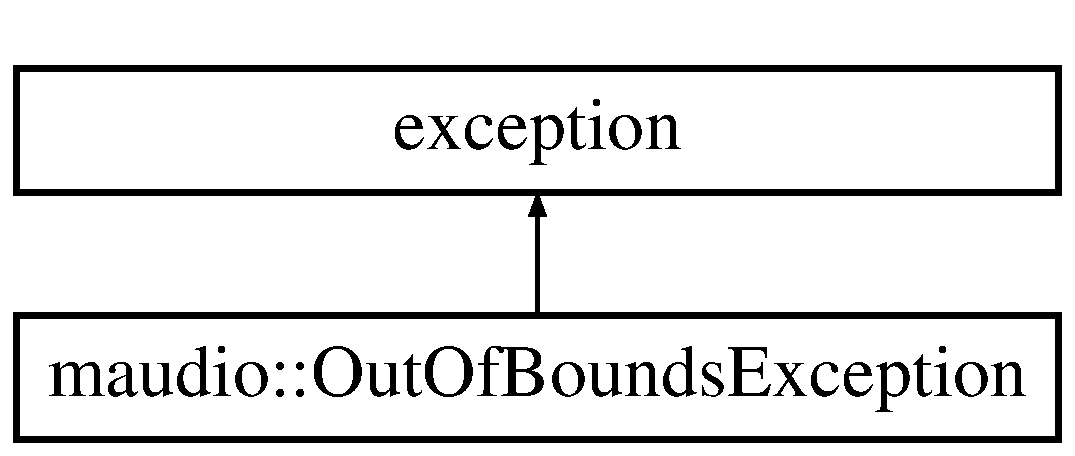
\includegraphics[height=2.000000cm]{classmaudio_1_1OutOfBoundsException}
\end{center}
\end{figure}
\subsection*{Public Member Functions}
\begin{DoxyCompactItemize}
\item 
virtual const char $\ast$ \hyperlink{classmaudio_1_1OutOfBoundsException_ad0b85a6a2fdf4534f1514cd5627a0975}{what} () const   throw ()
\end{DoxyCompactItemize}


\subsection{Member Function Documentation}
\hypertarget{classmaudio_1_1OutOfBoundsException_ad0b85a6a2fdf4534f1514cd5627a0975}{\index{maudio\-::\-Out\-Of\-Bounds\-Exception@{maudio\-::\-Out\-Of\-Bounds\-Exception}!what@{what}}
\index{what@{what}!maudio::OutOfBoundsException@{maudio\-::\-Out\-Of\-Bounds\-Exception}}
\subsubsection[{what}]{\setlength{\rightskip}{0pt plus 5cm}virtual const char$\ast$ maudio\-::\-Out\-Of\-Bounds\-Exception\-::what (
\begin{DoxyParamCaption}
{}
\end{DoxyParamCaption}
) const throw  ) \hspace{0.3cm}{\ttfamily [inline]}, {\ttfamily [virtual]}}}\label{classmaudio_1_1OutOfBoundsException_ad0b85a6a2fdf4534f1514cd5627a0975}


The documentation for this class was generated from the following file\-:\begin{DoxyCompactItemize}
\item 
/home/mars/\-Projekte/maudio/src/plugins/include/core/util/\hyperlink{AudioException_8hpp}{Audio\-Exception.\-hpp}\end{DoxyCompactItemize}

\hypertarget{classmaudio_1_1PlayerException}{\section{maudio\-:\-:Player\-Exception Class Reference}
\label{classmaudio_1_1PlayerException}\index{maudio\-::\-Player\-Exception@{maudio\-::\-Player\-Exception}}
}


{\ttfamily \#include $<$Audio\-Exception.\-hpp$>$}

Inheritance diagram for maudio\-:\-:Player\-Exception\-:\begin{figure}[H]
\begin{center}
\leavevmode
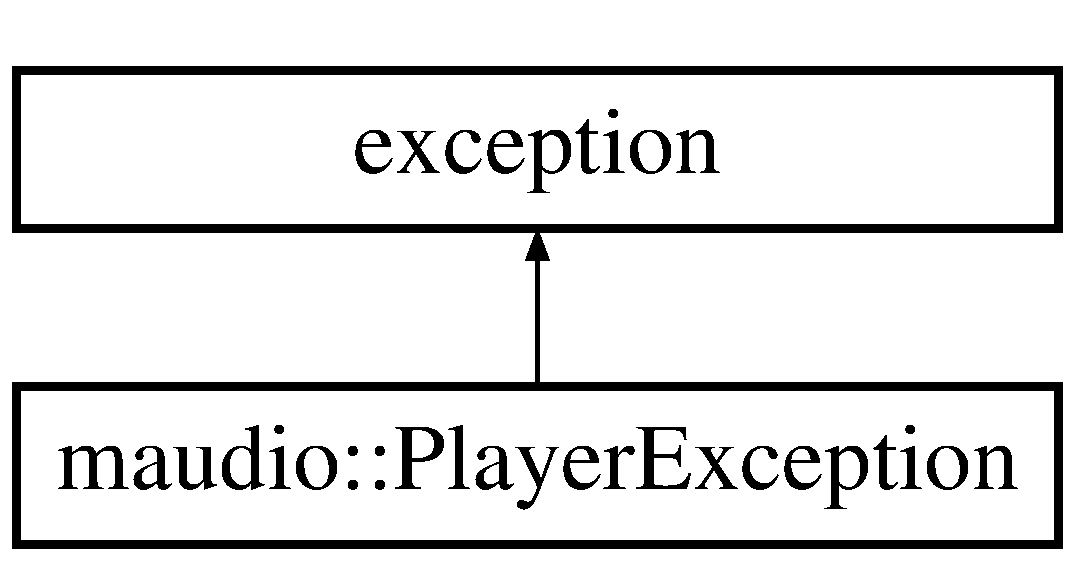
\includegraphics[height=2.000000cm]{classmaudio_1_1PlayerException}
\end{center}
\end{figure}
\subsection*{Public Member Functions}
\begin{DoxyCompactItemize}
\item 
virtual const char $\ast$ \hyperlink{classmaudio_1_1PlayerException_a6eb436f0cd083474e28fc6287856bf53}{what} () const   throw ()
\end{DoxyCompactItemize}


\subsection{Member Function Documentation}
\hypertarget{classmaudio_1_1PlayerException_a6eb436f0cd083474e28fc6287856bf53}{\index{maudio\-::\-Player\-Exception@{maudio\-::\-Player\-Exception}!what@{what}}
\index{what@{what}!maudio::PlayerException@{maudio\-::\-Player\-Exception}}
\subsubsection[{what}]{\setlength{\rightskip}{0pt plus 5cm}virtual const char$\ast$ maudio\-::\-Player\-Exception\-::what (
\begin{DoxyParamCaption}
{}
\end{DoxyParamCaption}
) const throw  ) \hspace{0.3cm}{\ttfamily [inline]}, {\ttfamily [virtual]}}}\label{classmaudio_1_1PlayerException_a6eb436f0cd083474e28fc6287856bf53}


The documentation for this class was generated from the following file\-:\begin{DoxyCompactItemize}
\item 
/home/mars/\-Projekte/maudio/src/plugins/include/core/util/\hyperlink{AudioException_8hpp}{Audio\-Exception.\-hpp}\end{DoxyCompactItemize}

\hypertarget{classmaudio_1_1PropertyManager}{\section{maudio\-:\-:Property\-Manager Class Reference}
\label{classmaudio_1_1PropertyManager}\index{maudio\-::\-Property\-Manager@{maudio\-::\-Property\-Manager}}
}


{\ttfamily \#include $<$Property\-Manager.\-hpp$>$}

Inheritance diagram for maudio\-:\-:Property\-Manager\-:\begin{figure}[H]
\begin{center}
\leavevmode
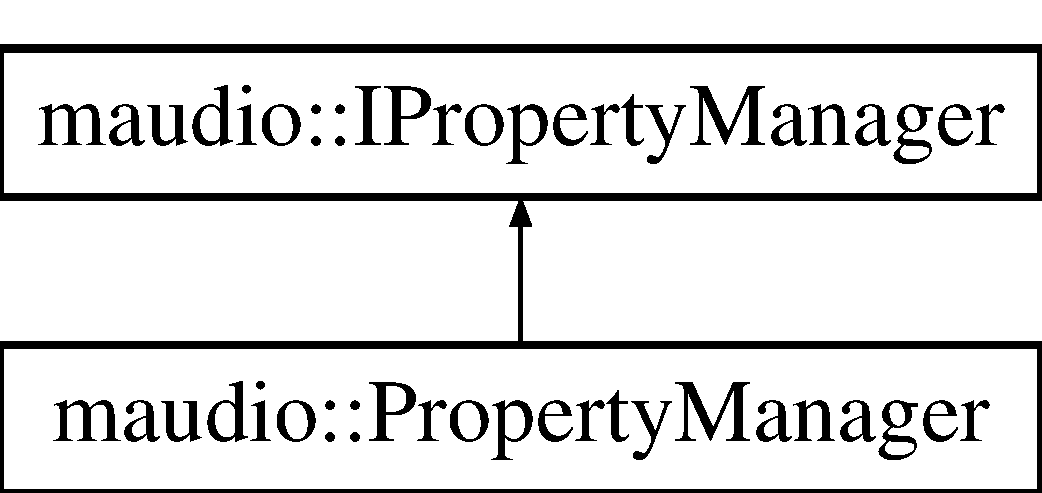
\includegraphics[height=2.000000cm]{classmaudio_1_1PropertyManager}
\end{center}
\end{figure}
\subsection*{Public Member Functions}
\begin{DoxyCompactItemize}
\item 
\hyperlink{classmaudio_1_1PropertyManager_ade281312fa768168d5b678332ad00175}{Property\-Manager} ()
\item 
virtual \hyperlink{classmaudio_1_1PropertyManager_a14129700c189235585c2c9ed2d637626}{$\sim$\-Property\-Manager} ()
\item 
virtual void \hyperlink{classmaudio_1_1PropertyManager_a247f345f6b91df3269d0032a7eadc78d}{add} (\hyperlink{classmaudio_1_1IProperty}{I\-Property} $\ast$prop)
\item 
virtual void \hyperlink{classmaudio_1_1PropertyManager_a01820518f68793e5c2f9a2720b962bae}{add} (\hyperlink{classmaudio_1_1IKeyableProperty}{I\-Keyable\-Property} $\ast$prop)
\item 
virtual bool \hyperlink{classmaudio_1_1PropertyManager_a0bb59c88f642ec5d24fa3c1c991378ed}{Property\-Exists} (const char $\ast$name)
\item 
virtual bool \hyperlink{classmaudio_1_1PropertyManager_a2d21e0f5b613771d721d21e35d30dca2}{Keyable\-Property\-Exists} (const char $\ast$name)
\item 
virtual \hyperlink{classmaudio_1_1IProperty}{I\-Property} $\ast$ \hyperlink{classmaudio_1_1PropertyManager_ad2d108b698b9e61f881670a9f5ce5132}{get\-Property} (unsigned int i)
\item 
virtual \hyperlink{classmaudio_1_1IProperty}{I\-Property} $\ast$ \hyperlink{classmaudio_1_1PropertyManager_ab947ffa97971be8b44047d444a99c65f}{get\-Property} (const char $\ast$name)
\item 
virtual \hyperlink{classmaudio_1_1IKeyableProperty}{I\-Keyable\-Property} $\ast$ \hyperlink{classmaudio_1_1PropertyManager_a6e1fe28a2f4d92cde3f3bb0d60ce4666}{get\-Keyable\-Property} (unsigned int i)
\item 
virtual \hyperlink{classmaudio_1_1IKeyableProperty}{I\-Keyable\-Property} $\ast$ \hyperlink{classmaudio_1_1PropertyManager_a5c9dbb27aef129bb1f23fb1d2eca6af3}{get\-Keyable\-Property} (const char $\ast$name)
\item 
virtual void \hyperlink{classmaudio_1_1PropertyManager_aa4dc70e93cf8f59275ed25c1bcaa804c}{remove\-Property} (unsigned int i)
\item 
virtual void \hyperlink{classmaudio_1_1PropertyManager_a737ebb28d24c575ecff05c81556f0ae1}{remove\-Property} (const char $\ast$name)
\item 
virtual void \hyperlink{classmaudio_1_1PropertyManager_a15c0a2e042acc6170631c2139785eae6}{remove\-Keyable\-Property} (unsigned int i)
\item 
virtual void \hyperlink{classmaudio_1_1PropertyManager_afc5d658aa68cb326e60225818d128a89}{remove\-Keyable\-Property} (const char $\ast$name)
\item 
virtual unsigned int \hyperlink{classmaudio_1_1PropertyManager_a12bec217f1ba5d9c0dfd2c9d872f5701}{get\-Num\-Properties} () const 
\item 
virtual unsigned int \hyperlink{classmaudio_1_1PropertyManager_a27309f637c4ab28f45c1cd57381701d4}{get\-Num\-Keyable\-Properties} () const 
\end{DoxyCompactItemize}


\subsection{Constructor \& Destructor Documentation}
\hypertarget{classmaudio_1_1PropertyManager_ade281312fa768168d5b678332ad00175}{\index{maudio\-::\-Property\-Manager@{maudio\-::\-Property\-Manager}!Property\-Manager@{Property\-Manager}}
\index{Property\-Manager@{Property\-Manager}!maudio::PropertyManager@{maudio\-::\-Property\-Manager}}
\subsubsection[{Property\-Manager}]{\setlength{\rightskip}{0pt plus 5cm}maudio\-::\-Property\-Manager\-::\-Property\-Manager (
\begin{DoxyParamCaption}
{}
\end{DoxyParamCaption}
)}}\label{classmaudio_1_1PropertyManager_ade281312fa768168d5b678332ad00175}
\hypertarget{classmaudio_1_1PropertyManager_a14129700c189235585c2c9ed2d637626}{\index{maudio\-::\-Property\-Manager@{maudio\-::\-Property\-Manager}!$\sim$\-Property\-Manager@{$\sim$\-Property\-Manager}}
\index{$\sim$\-Property\-Manager@{$\sim$\-Property\-Manager}!maudio::PropertyManager@{maudio\-::\-Property\-Manager}}
\subsubsection[{$\sim$\-Property\-Manager}]{\setlength{\rightskip}{0pt plus 5cm}maudio\-::\-Property\-Manager\-::$\sim$\-Property\-Manager (
\begin{DoxyParamCaption}
{}
\end{DoxyParamCaption}
)\hspace{0.3cm}{\ttfamily [virtual]}}}\label{classmaudio_1_1PropertyManager_a14129700c189235585c2c9ed2d637626}


\subsection{Member Function Documentation}
\hypertarget{classmaudio_1_1PropertyManager_a247f345f6b91df3269d0032a7eadc78d}{\index{maudio\-::\-Property\-Manager@{maudio\-::\-Property\-Manager}!add@{add}}
\index{add@{add}!maudio::PropertyManager@{maudio\-::\-Property\-Manager}}
\subsubsection[{add}]{\setlength{\rightskip}{0pt plus 5cm}void maudio\-::\-Property\-Manager\-::add (
\begin{DoxyParamCaption}
\item[{{\bf I\-Property} $\ast$}]{prop}
\end{DoxyParamCaption}
)\hspace{0.3cm}{\ttfamily [virtual]}}}\label{classmaudio_1_1PropertyManager_a247f345f6b91df3269d0032a7eadc78d}


Implements \hyperlink{classmaudio_1_1IPropertyManager_a6f1c1a5a3e9714e8ab22b73a5f67807e}{maudio\-::\-I\-Property\-Manager}.

\hypertarget{classmaudio_1_1PropertyManager_a01820518f68793e5c2f9a2720b962bae}{\index{maudio\-::\-Property\-Manager@{maudio\-::\-Property\-Manager}!add@{add}}
\index{add@{add}!maudio::PropertyManager@{maudio\-::\-Property\-Manager}}
\subsubsection[{add}]{\setlength{\rightskip}{0pt plus 5cm}void maudio\-::\-Property\-Manager\-::add (
\begin{DoxyParamCaption}
\item[{{\bf I\-Keyable\-Property} $\ast$}]{prop}
\end{DoxyParamCaption}
)\hspace{0.3cm}{\ttfamily [virtual]}}}\label{classmaudio_1_1PropertyManager_a01820518f68793e5c2f9a2720b962bae}


Implements \hyperlink{classmaudio_1_1IPropertyManager_a719bb2f8d8fb55126c7dc6d264600768}{maudio\-::\-I\-Property\-Manager}.

\hypertarget{classmaudio_1_1PropertyManager_a6e1fe28a2f4d92cde3f3bb0d60ce4666}{\index{maudio\-::\-Property\-Manager@{maudio\-::\-Property\-Manager}!get\-Keyable\-Property@{get\-Keyable\-Property}}
\index{get\-Keyable\-Property@{get\-Keyable\-Property}!maudio::PropertyManager@{maudio\-::\-Property\-Manager}}
\subsubsection[{get\-Keyable\-Property}]{\setlength{\rightskip}{0pt plus 5cm}{\bf I\-Keyable\-Property} $\ast$ maudio\-::\-Property\-Manager\-::get\-Keyable\-Property (
\begin{DoxyParamCaption}
\item[{unsigned int}]{i}
\end{DoxyParamCaption}
)\hspace{0.3cm}{\ttfamily [virtual]}}}\label{classmaudio_1_1PropertyManager_a6e1fe28a2f4d92cde3f3bb0d60ce4666}


Implements \hyperlink{classmaudio_1_1IPropertyManager_a68747539c9a666215de88337998b45d7}{maudio\-::\-I\-Property\-Manager}.

\hypertarget{classmaudio_1_1PropertyManager_a5c9dbb27aef129bb1f23fb1d2eca6af3}{\index{maudio\-::\-Property\-Manager@{maudio\-::\-Property\-Manager}!get\-Keyable\-Property@{get\-Keyable\-Property}}
\index{get\-Keyable\-Property@{get\-Keyable\-Property}!maudio::PropertyManager@{maudio\-::\-Property\-Manager}}
\subsubsection[{get\-Keyable\-Property}]{\setlength{\rightskip}{0pt plus 5cm}{\bf I\-Keyable\-Property} $\ast$ maudio\-::\-Property\-Manager\-::get\-Keyable\-Property (
\begin{DoxyParamCaption}
\item[{const char $\ast$}]{name}
\end{DoxyParamCaption}
)\hspace{0.3cm}{\ttfamily [virtual]}}}\label{classmaudio_1_1PropertyManager_a5c9dbb27aef129bb1f23fb1d2eca6af3}


Implements \hyperlink{classmaudio_1_1IPropertyManager_ac53ff45a9a42e265fa0d044a09bcc2ae}{maudio\-::\-I\-Property\-Manager}.

\hypertarget{classmaudio_1_1PropertyManager_a27309f637c4ab28f45c1cd57381701d4}{\index{maudio\-::\-Property\-Manager@{maudio\-::\-Property\-Manager}!get\-Num\-Keyable\-Properties@{get\-Num\-Keyable\-Properties}}
\index{get\-Num\-Keyable\-Properties@{get\-Num\-Keyable\-Properties}!maudio::PropertyManager@{maudio\-::\-Property\-Manager}}
\subsubsection[{get\-Num\-Keyable\-Properties}]{\setlength{\rightskip}{0pt plus 5cm}unsigned int maudio\-::\-Property\-Manager\-::get\-Num\-Keyable\-Properties (
\begin{DoxyParamCaption}
{}
\end{DoxyParamCaption}
) const\hspace{0.3cm}{\ttfamily [virtual]}}}\label{classmaudio_1_1PropertyManager_a27309f637c4ab28f45c1cd57381701d4}


Implements \hyperlink{classmaudio_1_1IPropertyManager_a7f7f9bab86f9972dadc0313589a2f07a}{maudio\-::\-I\-Property\-Manager}.

\hypertarget{classmaudio_1_1PropertyManager_a12bec217f1ba5d9c0dfd2c9d872f5701}{\index{maudio\-::\-Property\-Manager@{maudio\-::\-Property\-Manager}!get\-Num\-Properties@{get\-Num\-Properties}}
\index{get\-Num\-Properties@{get\-Num\-Properties}!maudio::PropertyManager@{maudio\-::\-Property\-Manager}}
\subsubsection[{get\-Num\-Properties}]{\setlength{\rightskip}{0pt plus 5cm}unsigned int maudio\-::\-Property\-Manager\-::get\-Num\-Properties (
\begin{DoxyParamCaption}
{}
\end{DoxyParamCaption}
) const\hspace{0.3cm}{\ttfamily [virtual]}}}\label{classmaudio_1_1PropertyManager_a12bec217f1ba5d9c0dfd2c9d872f5701}


Implements \hyperlink{classmaudio_1_1IPropertyManager_a27d2e238fc13c322941a21ef0c2aa04a}{maudio\-::\-I\-Property\-Manager}.

\hypertarget{classmaudio_1_1PropertyManager_ad2d108b698b9e61f881670a9f5ce5132}{\index{maudio\-::\-Property\-Manager@{maudio\-::\-Property\-Manager}!get\-Property@{get\-Property}}
\index{get\-Property@{get\-Property}!maudio::PropertyManager@{maudio\-::\-Property\-Manager}}
\subsubsection[{get\-Property}]{\setlength{\rightskip}{0pt plus 5cm}{\bf I\-Property} $\ast$ maudio\-::\-Property\-Manager\-::get\-Property (
\begin{DoxyParamCaption}
\item[{unsigned int}]{i}
\end{DoxyParamCaption}
)\hspace{0.3cm}{\ttfamily [virtual]}}}\label{classmaudio_1_1PropertyManager_ad2d108b698b9e61f881670a9f5ce5132}


Implements \hyperlink{classmaudio_1_1IPropertyManager_af25154a1f612b2bc44e40304290615ef}{maudio\-::\-I\-Property\-Manager}.

\hypertarget{classmaudio_1_1PropertyManager_ab947ffa97971be8b44047d444a99c65f}{\index{maudio\-::\-Property\-Manager@{maudio\-::\-Property\-Manager}!get\-Property@{get\-Property}}
\index{get\-Property@{get\-Property}!maudio::PropertyManager@{maudio\-::\-Property\-Manager}}
\subsubsection[{get\-Property}]{\setlength{\rightskip}{0pt plus 5cm}{\bf I\-Property} $\ast$ maudio\-::\-Property\-Manager\-::get\-Property (
\begin{DoxyParamCaption}
\item[{const char $\ast$}]{name}
\end{DoxyParamCaption}
)\hspace{0.3cm}{\ttfamily [virtual]}}}\label{classmaudio_1_1PropertyManager_ab947ffa97971be8b44047d444a99c65f}


Implements \hyperlink{classmaudio_1_1IPropertyManager_acbaea1cbdc990b9b4b0416a5c35d9435}{maudio\-::\-I\-Property\-Manager}.

\hypertarget{classmaudio_1_1PropertyManager_a2d21e0f5b613771d721d21e35d30dca2}{\index{maudio\-::\-Property\-Manager@{maudio\-::\-Property\-Manager}!Keyable\-Property\-Exists@{Keyable\-Property\-Exists}}
\index{Keyable\-Property\-Exists@{Keyable\-Property\-Exists}!maudio::PropertyManager@{maudio\-::\-Property\-Manager}}
\subsubsection[{Keyable\-Property\-Exists}]{\setlength{\rightskip}{0pt plus 5cm}bool maudio\-::\-Property\-Manager\-::\-Keyable\-Property\-Exists (
\begin{DoxyParamCaption}
\item[{const char $\ast$}]{name}
\end{DoxyParamCaption}
)\hspace{0.3cm}{\ttfamily [virtual]}}}\label{classmaudio_1_1PropertyManager_a2d21e0f5b613771d721d21e35d30dca2}


Implements \hyperlink{classmaudio_1_1IPropertyManager_a95f90f98cff9992a48fabe61168c95fb}{maudio\-::\-I\-Property\-Manager}.

\hypertarget{classmaudio_1_1PropertyManager_a0bb59c88f642ec5d24fa3c1c991378ed}{\index{maudio\-::\-Property\-Manager@{maudio\-::\-Property\-Manager}!Property\-Exists@{Property\-Exists}}
\index{Property\-Exists@{Property\-Exists}!maudio::PropertyManager@{maudio\-::\-Property\-Manager}}
\subsubsection[{Property\-Exists}]{\setlength{\rightskip}{0pt plus 5cm}bool maudio\-::\-Property\-Manager\-::\-Property\-Exists (
\begin{DoxyParamCaption}
\item[{const char $\ast$}]{name}
\end{DoxyParamCaption}
)\hspace{0.3cm}{\ttfamily [virtual]}}}\label{classmaudio_1_1PropertyManager_a0bb59c88f642ec5d24fa3c1c991378ed}


Implements \hyperlink{classmaudio_1_1IPropertyManager_a0d2b0d87656c2eb7e93ca867848d1559}{maudio\-::\-I\-Property\-Manager}.

\hypertarget{classmaudio_1_1PropertyManager_a15c0a2e042acc6170631c2139785eae6}{\index{maudio\-::\-Property\-Manager@{maudio\-::\-Property\-Manager}!remove\-Keyable\-Property@{remove\-Keyable\-Property}}
\index{remove\-Keyable\-Property@{remove\-Keyable\-Property}!maudio::PropertyManager@{maudio\-::\-Property\-Manager}}
\subsubsection[{remove\-Keyable\-Property}]{\setlength{\rightskip}{0pt plus 5cm}void maudio\-::\-Property\-Manager\-::remove\-Keyable\-Property (
\begin{DoxyParamCaption}
\item[{unsigned int}]{i}
\end{DoxyParamCaption}
)\hspace{0.3cm}{\ttfamily [virtual]}}}\label{classmaudio_1_1PropertyManager_a15c0a2e042acc6170631c2139785eae6}


Implements \hyperlink{classmaudio_1_1IPropertyManager_a6fbce7ab4d22a147fba13d54be8c6328}{maudio\-::\-I\-Property\-Manager}.

\hypertarget{classmaudio_1_1PropertyManager_afc5d658aa68cb326e60225818d128a89}{\index{maudio\-::\-Property\-Manager@{maudio\-::\-Property\-Manager}!remove\-Keyable\-Property@{remove\-Keyable\-Property}}
\index{remove\-Keyable\-Property@{remove\-Keyable\-Property}!maudio::PropertyManager@{maudio\-::\-Property\-Manager}}
\subsubsection[{remove\-Keyable\-Property}]{\setlength{\rightskip}{0pt plus 5cm}void maudio\-::\-Property\-Manager\-::remove\-Keyable\-Property (
\begin{DoxyParamCaption}
\item[{const char $\ast$}]{name}
\end{DoxyParamCaption}
)\hspace{0.3cm}{\ttfamily [virtual]}}}\label{classmaudio_1_1PropertyManager_afc5d658aa68cb326e60225818d128a89}


Implements \hyperlink{classmaudio_1_1IPropertyManager_a31ab51fa15263b7aa67a6a0dd1f91985}{maudio\-::\-I\-Property\-Manager}.

\hypertarget{classmaudio_1_1PropertyManager_aa4dc70e93cf8f59275ed25c1bcaa804c}{\index{maudio\-::\-Property\-Manager@{maudio\-::\-Property\-Manager}!remove\-Property@{remove\-Property}}
\index{remove\-Property@{remove\-Property}!maudio::PropertyManager@{maudio\-::\-Property\-Manager}}
\subsubsection[{remove\-Property}]{\setlength{\rightskip}{0pt plus 5cm}void maudio\-::\-Property\-Manager\-::remove\-Property (
\begin{DoxyParamCaption}
\item[{unsigned int}]{i}
\end{DoxyParamCaption}
)\hspace{0.3cm}{\ttfamily [virtual]}}}\label{classmaudio_1_1PropertyManager_aa4dc70e93cf8f59275ed25c1bcaa804c}


Implements \hyperlink{classmaudio_1_1IPropertyManager_aedc3df4a29c0ae8d137ac29b5b0abbf1}{maudio\-::\-I\-Property\-Manager}.

\hypertarget{classmaudio_1_1PropertyManager_a737ebb28d24c575ecff05c81556f0ae1}{\index{maudio\-::\-Property\-Manager@{maudio\-::\-Property\-Manager}!remove\-Property@{remove\-Property}}
\index{remove\-Property@{remove\-Property}!maudio::PropertyManager@{maudio\-::\-Property\-Manager}}
\subsubsection[{remove\-Property}]{\setlength{\rightskip}{0pt plus 5cm}void maudio\-::\-Property\-Manager\-::remove\-Property (
\begin{DoxyParamCaption}
\item[{const char $\ast$}]{name}
\end{DoxyParamCaption}
)\hspace{0.3cm}{\ttfamily [virtual]}}}\label{classmaudio_1_1PropertyManager_a737ebb28d24c575ecff05c81556f0ae1}


Implements \hyperlink{classmaudio_1_1IPropertyManager_a41d9333efef184d05a1e1c929097059f}{maudio\-::\-I\-Property\-Manager}.



The documentation for this class was generated from the following files\-:\begin{DoxyCompactItemize}
\item 
/home/mars/\-Projekte/maudio/src/plugins/include/core/property/\hyperlink{PropertyManager_8hpp}{Property\-Manager.\-hpp}\item 
/home/mars/\-Projekte/maudio/src/core/property/\hyperlink{core_2property_2PropertyManager_8cpp}{Property\-Manager.\-cpp}\end{DoxyCompactItemize}

\hypertarget{classmaudio_1_1Sample}{\section{maudio\-:\-:Sample Class Reference}
\label{classmaudio_1_1Sample}\index{maudio\-::\-Sample@{maudio\-::\-Sample}}
}


Holds a sample of audio.  




{\ttfamily \#include $<$Sample.\-hpp$>$}

Inheritance diagram for maudio\-:\-:Sample\-:\begin{figure}[H]
\begin{center}
\leavevmode
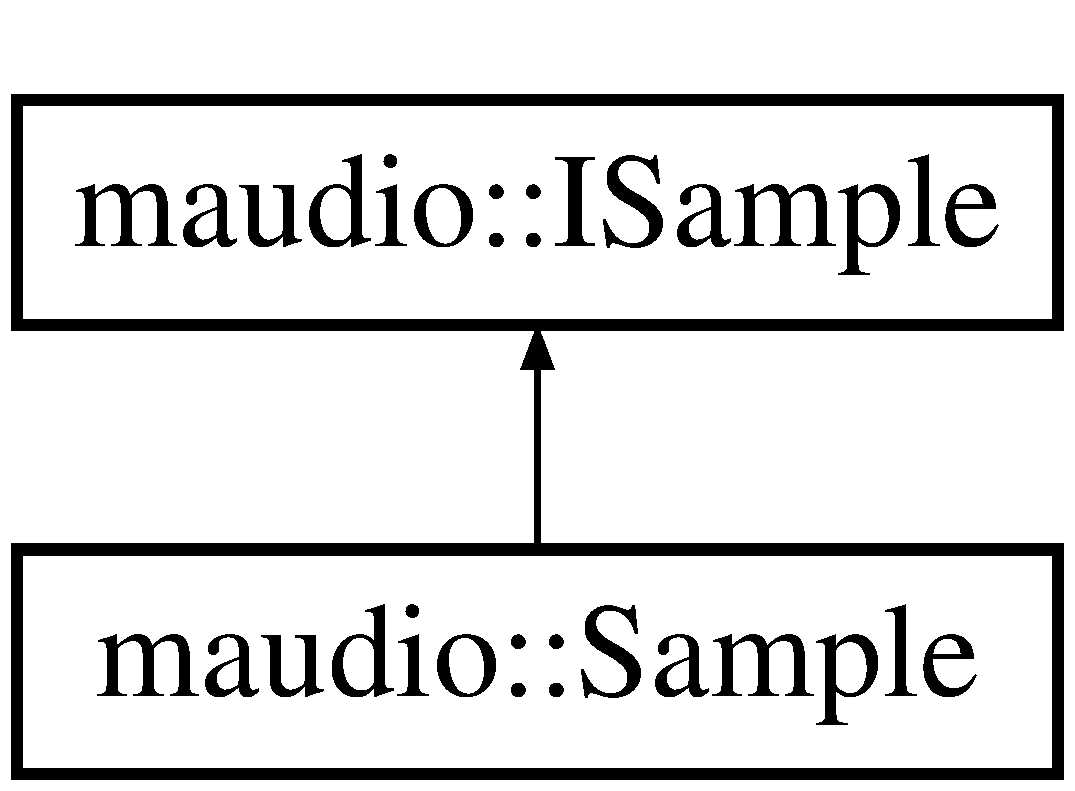
\includegraphics[height=2.000000cm]{classmaudio_1_1Sample}
\end{center}
\end{figure}
\subsection*{Public Member Functions}
\begin{DoxyCompactItemize}
\item 
\hyperlink{classmaudio_1_1Sample_a4a18ac0617d8af885f173fac6a64d99e}{Sample} (unsigned int channels)
\item 
\hyperlink{classmaudio_1_1Sample_a46a4149c6c4facdb2c961896dee3d9b9}{Sample} (const std\-::vector$<$ float $>$ data)
\item 
\hyperlink{classmaudio_1_1Sample_a380515efa355237efefe53a4b4ab80b5}{Sample} (const \hyperlink{classmaudio_1_1ISample}{I\-Sample} \&data)
\item 
virtual \hyperlink{classmaudio_1_1Sample_a51b823c9794d373f72d9471edaf5f9c3}{$\sim$\-Sample} ()
\item 
virtual const float \hyperlink{classmaudio_1_1Sample_afb3132c845a9254cab792c704f163e10}{operator\mbox{[}$\,$\mbox{]}} (unsigned int pos) const 
\item 
virtual void \hyperlink{classmaudio_1_1Sample_af3e4beb689ca243a5f1da0b32c1e8931}{operator=} (const \hyperlink{classmaudio_1_1ISample}{I\-Sample} \&data)
\item 
virtual float \hyperlink{classmaudio_1_1Sample_abc1d709a5c730747aa155109a11d99ce}{get} (unsigned int pos) const 
\item 
virtual void \hyperlink{classmaudio_1_1Sample_a3e934051125c16e499d04bdb974e9f44}{set} (float data, unsigned int pos)
\item 
virtual unsigned int \hyperlink{classmaudio_1_1Sample_a30b228a9490d8afa6dfdcf34d44553c3}{get\-Channels} () const 
\item 
virtual \hyperlink{classmaudio_1_1ISample}{I\-Sample} $\ast$ \hyperlink{classmaudio_1_1Sample_a3784ec5b915e1a06f76af431cf2d51e3}{operator+} (const \hyperlink{classmaudio_1_1ISample}{I\-Sample} \&data)
\item 
virtual \hyperlink{classmaudio_1_1ISample}{I\-Sample} $\ast$ \hyperlink{classmaudio_1_1Sample_af6fab639be30873ff867c95be407ea6e}{operator-\/} (const \hyperlink{classmaudio_1_1ISample}{I\-Sample} \&data)
\item 
virtual \hyperlink{classmaudio_1_1ISample}{I\-Sample} $\ast$ \hyperlink{classmaudio_1_1Sample_a1b7626f92fc63060bbbe718a57a801d8}{operator$\ast$} (const \hyperlink{classmaudio_1_1ISample}{I\-Sample} \&data)
\item 
virtual \hyperlink{classmaudio_1_1ISample}{I\-Sample} $\ast$ \hyperlink{classmaudio_1_1Sample_aa0fc9649f0c195a614a57e5be2092b5c}{operator/} (const \hyperlink{classmaudio_1_1ISample}{I\-Sample} \&data)
\item 
virtual \hyperlink{classmaudio_1_1ISample}{I\-Sample} $\ast$ \hyperlink{classmaudio_1_1Sample_a3acd28e07a7fd552a54f6a0755493056}{operator$\ast$} (float data)
\item 
virtual \hyperlink{classmaudio_1_1ISample}{I\-Sample} $\ast$ \hyperlink{classmaudio_1_1Sample_ade7a0f4a21b0b78f082ee4c09c983d7c}{operator/} (float data)
\item 
virtual void \hyperlink{classmaudio_1_1Sample_aaaa4dcbd04db90aa9bdcf3f63665a9c7}{operator+=} (const \hyperlink{classmaudio_1_1ISample}{I\-Sample} \&data)
\item 
virtual void \hyperlink{classmaudio_1_1Sample_a2cf98ca0a69364efb1f9b3a083bacff5}{operator-\/=} (const \hyperlink{classmaudio_1_1ISample}{I\-Sample} \&data)
\item 
virtual void \hyperlink{classmaudio_1_1Sample_a48654599874e90747f0e2df36e8a5038}{operator$\ast$=} (const \hyperlink{classmaudio_1_1ISample}{I\-Sample} \&data)
\item 
virtual void \hyperlink{classmaudio_1_1Sample_aecb80004ebd611674563fe1c0aadb860}{operator/=} (const \hyperlink{classmaudio_1_1ISample}{I\-Sample} \&data)
\item 
virtual void \hyperlink{classmaudio_1_1Sample_a3ae8257702e07cc7af3424bbc04feede}{operator$\ast$=} (float data)
\item 
virtual void \hyperlink{classmaudio_1_1Sample_ac7b187b92806613e71bf4fccebf65bff}{operator/=} (float data)
\end{DoxyCompactItemize}


\subsection{Detailed Description}
Holds a sample of audio. 

\subsection{Constructor \& Destructor Documentation}
\hypertarget{classmaudio_1_1Sample_a4a18ac0617d8af885f173fac6a64d99e}{\index{maudio\-::\-Sample@{maudio\-::\-Sample}!Sample@{Sample}}
\index{Sample@{Sample}!maudio::Sample@{maudio\-::\-Sample}}
\subsubsection[{Sample}]{\setlength{\rightskip}{0pt plus 5cm}maudio\-::\-Sample\-::\-Sample (
\begin{DoxyParamCaption}
\item[{unsigned int}]{channels}
\end{DoxyParamCaption}
)}}\label{classmaudio_1_1Sample_a4a18ac0617d8af885f173fac6a64d99e}
\hypertarget{classmaudio_1_1Sample_a46a4149c6c4facdb2c961896dee3d9b9}{\index{maudio\-::\-Sample@{maudio\-::\-Sample}!Sample@{Sample}}
\index{Sample@{Sample}!maudio::Sample@{maudio\-::\-Sample}}
\subsubsection[{Sample}]{\setlength{\rightskip}{0pt plus 5cm}maudio\-::\-Sample\-::\-Sample (
\begin{DoxyParamCaption}
\item[{const std\-::vector$<$ float $>$}]{data}
\end{DoxyParamCaption}
)}}\label{classmaudio_1_1Sample_a46a4149c6c4facdb2c961896dee3d9b9}
\hypertarget{classmaudio_1_1Sample_a380515efa355237efefe53a4b4ab80b5}{\index{maudio\-::\-Sample@{maudio\-::\-Sample}!Sample@{Sample}}
\index{Sample@{Sample}!maudio::Sample@{maudio\-::\-Sample}}
\subsubsection[{Sample}]{\setlength{\rightskip}{0pt plus 5cm}maudio\-::\-Sample\-::\-Sample (
\begin{DoxyParamCaption}
\item[{const {\bf I\-Sample} \&}]{data}
\end{DoxyParamCaption}
)}}\label{classmaudio_1_1Sample_a380515efa355237efefe53a4b4ab80b5}
\hypertarget{classmaudio_1_1Sample_a51b823c9794d373f72d9471edaf5f9c3}{\index{maudio\-::\-Sample@{maudio\-::\-Sample}!$\sim$\-Sample@{$\sim$\-Sample}}
\index{$\sim$\-Sample@{$\sim$\-Sample}!maudio::Sample@{maudio\-::\-Sample}}
\subsubsection[{$\sim$\-Sample}]{\setlength{\rightskip}{0pt plus 5cm}maudio\-::\-Sample\-::$\sim$\-Sample (
\begin{DoxyParamCaption}
{}
\end{DoxyParamCaption}
)\hspace{0.3cm}{\ttfamily [virtual]}}}\label{classmaudio_1_1Sample_a51b823c9794d373f72d9471edaf5f9c3}


\subsection{Member Function Documentation}
\hypertarget{classmaudio_1_1Sample_abc1d709a5c730747aa155109a11d99ce}{\index{maudio\-::\-Sample@{maudio\-::\-Sample}!get@{get}}
\index{get@{get}!maudio::Sample@{maudio\-::\-Sample}}
\subsubsection[{get}]{\setlength{\rightskip}{0pt plus 5cm}float maudio\-::\-Sample\-::get (
\begin{DoxyParamCaption}
\item[{unsigned int}]{pos}
\end{DoxyParamCaption}
) const\hspace{0.3cm}{\ttfamily [virtual]}}}\label{classmaudio_1_1Sample_abc1d709a5c730747aa155109a11d99ce}


Implements \hyperlink{classmaudio_1_1ISample_a2a1eef822e43d5807a7ff3e9798783c6}{maudio\-::\-I\-Sample}.

\hypertarget{classmaudio_1_1Sample_a30b228a9490d8afa6dfdcf34d44553c3}{\index{maudio\-::\-Sample@{maudio\-::\-Sample}!get\-Channels@{get\-Channels}}
\index{get\-Channels@{get\-Channels}!maudio::Sample@{maudio\-::\-Sample}}
\subsubsection[{get\-Channels}]{\setlength{\rightskip}{0pt plus 5cm}unsigned int maudio\-::\-Sample\-::get\-Channels (
\begin{DoxyParamCaption}
{}
\end{DoxyParamCaption}
) const\hspace{0.3cm}{\ttfamily [virtual]}}}\label{classmaudio_1_1Sample_a30b228a9490d8afa6dfdcf34d44553c3}


Implements \hyperlink{classmaudio_1_1ISample_a2c05b7da59cc625f695352a11a81351c}{maudio\-::\-I\-Sample}.

\hypertarget{classmaudio_1_1Sample_a1b7626f92fc63060bbbe718a57a801d8}{\index{maudio\-::\-Sample@{maudio\-::\-Sample}!operator$\ast$@{operator$\ast$}}
\index{operator$\ast$@{operator$\ast$}!maudio::Sample@{maudio\-::\-Sample}}
\subsubsection[{operator$\ast$}]{\setlength{\rightskip}{0pt plus 5cm}{\bf I\-Sample} $\ast$ maudio\-::\-Sample\-::operator$\ast$ (
\begin{DoxyParamCaption}
\item[{const {\bf I\-Sample} \&}]{data}
\end{DoxyParamCaption}
)\hspace{0.3cm}{\ttfamily [virtual]}}}\label{classmaudio_1_1Sample_a1b7626f92fc63060bbbe718a57a801d8}


Implements \hyperlink{classmaudio_1_1ISample_aa7dcb9e5e605bb8b3bb18c0d64d0f98f}{maudio\-::\-I\-Sample}.

\hypertarget{classmaudio_1_1Sample_a3acd28e07a7fd552a54f6a0755493056}{\index{maudio\-::\-Sample@{maudio\-::\-Sample}!operator$\ast$@{operator$\ast$}}
\index{operator$\ast$@{operator$\ast$}!maudio::Sample@{maudio\-::\-Sample}}
\subsubsection[{operator$\ast$}]{\setlength{\rightskip}{0pt plus 5cm}{\bf I\-Sample} $\ast$ maudio\-::\-Sample\-::operator$\ast$ (
\begin{DoxyParamCaption}
\item[{float}]{data}
\end{DoxyParamCaption}
)\hspace{0.3cm}{\ttfamily [virtual]}}}\label{classmaudio_1_1Sample_a3acd28e07a7fd552a54f6a0755493056}


Implements \hyperlink{classmaudio_1_1ISample_ace42669d0bb902e6237c6aa491f3177d}{maudio\-::\-I\-Sample}.

\hypertarget{classmaudio_1_1Sample_a48654599874e90747f0e2df36e8a5038}{\index{maudio\-::\-Sample@{maudio\-::\-Sample}!operator$\ast$=@{operator$\ast$=}}
\index{operator$\ast$=@{operator$\ast$=}!maudio::Sample@{maudio\-::\-Sample}}
\subsubsection[{operator$\ast$=}]{\setlength{\rightskip}{0pt plus 5cm}void maudio\-::\-Sample\-::operator$\ast$= (
\begin{DoxyParamCaption}
\item[{const {\bf I\-Sample} \&}]{data}
\end{DoxyParamCaption}
)\hspace{0.3cm}{\ttfamily [virtual]}}}\label{classmaudio_1_1Sample_a48654599874e90747f0e2df36e8a5038}


Implements \hyperlink{classmaudio_1_1ISample_abc3eeb3d0432fcdb0cf2105d703a1b01}{maudio\-::\-I\-Sample}.

\hypertarget{classmaudio_1_1Sample_a3ae8257702e07cc7af3424bbc04feede}{\index{maudio\-::\-Sample@{maudio\-::\-Sample}!operator$\ast$=@{operator$\ast$=}}
\index{operator$\ast$=@{operator$\ast$=}!maudio::Sample@{maudio\-::\-Sample}}
\subsubsection[{operator$\ast$=}]{\setlength{\rightskip}{0pt plus 5cm}void maudio\-::\-Sample\-::operator$\ast$= (
\begin{DoxyParamCaption}
\item[{float}]{data}
\end{DoxyParamCaption}
)\hspace{0.3cm}{\ttfamily [virtual]}}}\label{classmaudio_1_1Sample_a3ae8257702e07cc7af3424bbc04feede}


Implements \hyperlink{classmaudio_1_1ISample_ad3bd2552fb977ec53225cb37f09da3cd}{maudio\-::\-I\-Sample}.

\hypertarget{classmaudio_1_1Sample_a3784ec5b915e1a06f76af431cf2d51e3}{\index{maudio\-::\-Sample@{maudio\-::\-Sample}!operator+@{operator+}}
\index{operator+@{operator+}!maudio::Sample@{maudio\-::\-Sample}}
\subsubsection[{operator+}]{\setlength{\rightskip}{0pt plus 5cm}{\bf I\-Sample} $\ast$ maudio\-::\-Sample\-::operator+ (
\begin{DoxyParamCaption}
\item[{const {\bf I\-Sample} \&}]{data}
\end{DoxyParamCaption}
)\hspace{0.3cm}{\ttfamily [virtual]}}}\label{classmaudio_1_1Sample_a3784ec5b915e1a06f76af431cf2d51e3}


Implements \hyperlink{classmaudio_1_1ISample_abd3ff392a72c89576b111dd4120eb2b0}{maudio\-::\-I\-Sample}.

\hypertarget{classmaudio_1_1Sample_aaaa4dcbd04db90aa9bdcf3f63665a9c7}{\index{maudio\-::\-Sample@{maudio\-::\-Sample}!operator+=@{operator+=}}
\index{operator+=@{operator+=}!maudio::Sample@{maudio\-::\-Sample}}
\subsubsection[{operator+=}]{\setlength{\rightskip}{0pt plus 5cm}void maudio\-::\-Sample\-::operator+= (
\begin{DoxyParamCaption}
\item[{const {\bf I\-Sample} \&}]{data}
\end{DoxyParamCaption}
)\hspace{0.3cm}{\ttfamily [virtual]}}}\label{classmaudio_1_1Sample_aaaa4dcbd04db90aa9bdcf3f63665a9c7}


Implements \hyperlink{classmaudio_1_1ISample_a3000493ce6c2d3fccc88565360170ff7}{maudio\-::\-I\-Sample}.

\hypertarget{classmaudio_1_1Sample_af6fab639be30873ff867c95be407ea6e}{\index{maudio\-::\-Sample@{maudio\-::\-Sample}!operator-\/@{operator-\/}}
\index{operator-\/@{operator-\/}!maudio::Sample@{maudio\-::\-Sample}}
\subsubsection[{operator-\/}]{\setlength{\rightskip}{0pt plus 5cm}{\bf I\-Sample} $\ast$ maudio\-::\-Sample\-::operator-\/ (
\begin{DoxyParamCaption}
\item[{const {\bf I\-Sample} \&}]{data}
\end{DoxyParamCaption}
)\hspace{0.3cm}{\ttfamily [virtual]}}}\label{classmaudio_1_1Sample_af6fab639be30873ff867c95be407ea6e}


Implements \hyperlink{classmaudio_1_1ISample_a654eb71ce13136f6f8a1299daab81a85}{maudio\-::\-I\-Sample}.

\hypertarget{classmaudio_1_1Sample_a2cf98ca0a69364efb1f9b3a083bacff5}{\index{maudio\-::\-Sample@{maudio\-::\-Sample}!operator-\/=@{operator-\/=}}
\index{operator-\/=@{operator-\/=}!maudio::Sample@{maudio\-::\-Sample}}
\subsubsection[{operator-\/=}]{\setlength{\rightskip}{0pt plus 5cm}void maudio\-::\-Sample\-::operator-\/= (
\begin{DoxyParamCaption}
\item[{const {\bf I\-Sample} \&}]{data}
\end{DoxyParamCaption}
)\hspace{0.3cm}{\ttfamily [virtual]}}}\label{classmaudio_1_1Sample_a2cf98ca0a69364efb1f9b3a083bacff5}


Implements \hyperlink{classmaudio_1_1ISample_ac635182905ed788cd498b21b025b6fb4}{maudio\-::\-I\-Sample}.

\hypertarget{classmaudio_1_1Sample_aa0fc9649f0c195a614a57e5be2092b5c}{\index{maudio\-::\-Sample@{maudio\-::\-Sample}!operator/@{operator/}}
\index{operator/@{operator/}!maudio::Sample@{maudio\-::\-Sample}}
\subsubsection[{operator/}]{\setlength{\rightskip}{0pt plus 5cm}{\bf I\-Sample} $\ast$ maudio\-::\-Sample\-::operator/ (
\begin{DoxyParamCaption}
\item[{const {\bf I\-Sample} \&}]{data}
\end{DoxyParamCaption}
)\hspace{0.3cm}{\ttfamily [virtual]}}}\label{classmaudio_1_1Sample_aa0fc9649f0c195a614a57e5be2092b5c}


Implements \hyperlink{classmaudio_1_1ISample_a11fd4f5c355e90f67317881618289b4b}{maudio\-::\-I\-Sample}.

\hypertarget{classmaudio_1_1Sample_ade7a0f4a21b0b78f082ee4c09c983d7c}{\index{maudio\-::\-Sample@{maudio\-::\-Sample}!operator/@{operator/}}
\index{operator/@{operator/}!maudio::Sample@{maudio\-::\-Sample}}
\subsubsection[{operator/}]{\setlength{\rightskip}{0pt plus 5cm}{\bf I\-Sample} $\ast$ maudio\-::\-Sample\-::operator/ (
\begin{DoxyParamCaption}
\item[{float}]{data}
\end{DoxyParamCaption}
)\hspace{0.3cm}{\ttfamily [virtual]}}}\label{classmaudio_1_1Sample_ade7a0f4a21b0b78f082ee4c09c983d7c}


Implements \hyperlink{classmaudio_1_1ISample_a48dfc510f76abb0981c8edb79f737c09}{maudio\-::\-I\-Sample}.

\hypertarget{classmaudio_1_1Sample_aecb80004ebd611674563fe1c0aadb860}{\index{maudio\-::\-Sample@{maudio\-::\-Sample}!operator/=@{operator/=}}
\index{operator/=@{operator/=}!maudio::Sample@{maudio\-::\-Sample}}
\subsubsection[{operator/=}]{\setlength{\rightskip}{0pt plus 5cm}void maudio\-::\-Sample\-::operator/= (
\begin{DoxyParamCaption}
\item[{const {\bf I\-Sample} \&}]{data}
\end{DoxyParamCaption}
)\hspace{0.3cm}{\ttfamily [virtual]}}}\label{classmaudio_1_1Sample_aecb80004ebd611674563fe1c0aadb860}


Implements \hyperlink{classmaudio_1_1ISample_af9b70d20e42b6d8711e4a796c1ef260d}{maudio\-::\-I\-Sample}.

\hypertarget{classmaudio_1_1Sample_ac7b187b92806613e71bf4fccebf65bff}{\index{maudio\-::\-Sample@{maudio\-::\-Sample}!operator/=@{operator/=}}
\index{operator/=@{operator/=}!maudio::Sample@{maudio\-::\-Sample}}
\subsubsection[{operator/=}]{\setlength{\rightskip}{0pt plus 5cm}void maudio\-::\-Sample\-::operator/= (
\begin{DoxyParamCaption}
\item[{float}]{data}
\end{DoxyParamCaption}
)\hspace{0.3cm}{\ttfamily [virtual]}}}\label{classmaudio_1_1Sample_ac7b187b92806613e71bf4fccebf65bff}


Implements \hyperlink{classmaudio_1_1ISample_a1ade860d885977e6b1b333170ae5ec41}{maudio\-::\-I\-Sample}.

\hypertarget{classmaudio_1_1Sample_af3e4beb689ca243a5f1da0b32c1e8931}{\index{maudio\-::\-Sample@{maudio\-::\-Sample}!operator=@{operator=}}
\index{operator=@{operator=}!maudio::Sample@{maudio\-::\-Sample}}
\subsubsection[{operator=}]{\setlength{\rightskip}{0pt plus 5cm}void maudio\-::\-Sample\-::operator= (
\begin{DoxyParamCaption}
\item[{const {\bf I\-Sample} \&}]{data}
\end{DoxyParamCaption}
)\hspace{0.3cm}{\ttfamily [virtual]}}}\label{classmaudio_1_1Sample_af3e4beb689ca243a5f1da0b32c1e8931}
\hypertarget{classmaudio_1_1Sample_afb3132c845a9254cab792c704f163e10}{\index{maudio\-::\-Sample@{maudio\-::\-Sample}!operator\mbox{[}$\,$\mbox{]}@{operator[]}}
\index{operator\mbox{[}$\,$\mbox{]}@{operator[]}!maudio::Sample@{maudio\-::\-Sample}}
\subsubsection[{operator[]}]{\setlength{\rightskip}{0pt plus 5cm}const float maudio\-::\-Sample\-::operator\mbox{[}$\,$\mbox{]} (
\begin{DoxyParamCaption}
\item[{unsigned int}]{pos}
\end{DoxyParamCaption}
) const\hspace{0.3cm}{\ttfamily [virtual]}}}\label{classmaudio_1_1Sample_afb3132c845a9254cab792c704f163e10}


Implements \hyperlink{classmaudio_1_1ISample_ad90962cd3f480cbba7a891530371e405}{maudio\-::\-I\-Sample}.

\hypertarget{classmaudio_1_1Sample_a3e934051125c16e499d04bdb974e9f44}{\index{maudio\-::\-Sample@{maudio\-::\-Sample}!set@{set}}
\index{set@{set}!maudio::Sample@{maudio\-::\-Sample}}
\subsubsection[{set}]{\setlength{\rightskip}{0pt plus 5cm}void maudio\-::\-Sample\-::set (
\begin{DoxyParamCaption}
\item[{float}]{data, }
\item[{unsigned int}]{pos}
\end{DoxyParamCaption}
)\hspace{0.3cm}{\ttfamily [virtual]}}}\label{classmaudio_1_1Sample_a3e934051125c16e499d04bdb974e9f44}


Implements \hyperlink{classmaudio_1_1ISample_a0b65702ea137559932feee764cfc190e}{maudio\-::\-I\-Sample}.



The documentation for this class was generated from the following files\-:\begin{DoxyCompactItemize}
\item 
/home/mars/\-Projekte/maudio/src/plugins/include/core/audiodata/\hyperlink{Sample_8hpp}{Sample.\-hpp}\item 
/home/mars/\-Projekte/maudio/src/core/audiodata/\hyperlink{core_2audiodata_2Sample_8cpp}{Sample.\-cpp}\end{DoxyCompactItemize}

\hypertarget{classmaudio_1_1Scene}{\section{maudio\-:\-:Scene Class Reference}
\label{classmaudio_1_1Scene}\index{maudio\-::\-Scene@{maudio\-::\-Scene}}
}


{\ttfamily \#include $<$Scene.\-hpp$>$}

\subsection*{Public Member Functions}
\begin{DoxyCompactItemize}
\item 
\hyperlink{classmaudio_1_1Scene_a4c4d3c71a4e076b3c5323dc1595b09fe}{Scene} ()
\item 
\hyperlink{classmaudio_1_1Scene_aa48f0b5004548eb1db57d10767f5d09d}{$\sim$\-Scene} ()
\end{DoxyCompactItemize}


\subsection{Constructor \& Destructor Documentation}
\hypertarget{classmaudio_1_1Scene_a4c4d3c71a4e076b3c5323dc1595b09fe}{\index{maudio\-::\-Scene@{maudio\-::\-Scene}!Scene@{Scene}}
\index{Scene@{Scene}!maudio::Scene@{maudio\-::\-Scene}}
\subsubsection[{Scene}]{\setlength{\rightskip}{0pt plus 5cm}maudio\-::\-Scene\-::\-Scene (
\begin{DoxyParamCaption}
{}
\end{DoxyParamCaption}
)}}\label{classmaudio_1_1Scene_a4c4d3c71a4e076b3c5323dc1595b09fe}
\hypertarget{classmaudio_1_1Scene_aa48f0b5004548eb1db57d10767f5d09d}{\index{maudio\-::\-Scene@{maudio\-::\-Scene}!$\sim$\-Scene@{$\sim$\-Scene}}
\index{$\sim$\-Scene@{$\sim$\-Scene}!maudio::Scene@{maudio\-::\-Scene}}
\subsubsection[{$\sim$\-Scene}]{\setlength{\rightskip}{0pt plus 5cm}maudio\-::\-Scene\-::$\sim$\-Scene (
\begin{DoxyParamCaption}
{}
\end{DoxyParamCaption}
)}}\label{classmaudio_1_1Scene_aa48f0b5004548eb1db57d10767f5d09d}


The documentation for this class was generated from the following file\-:\begin{DoxyCompactItemize}
\item 
/home/mars/\-Projekte/maudio/src/plugins/include/core/node/\hyperlink{Scene_8hpp}{Scene.\-hpp}\end{DoxyCompactItemize}

\hypertarget{classmaudio_1_1Serializer}{\section{maudio\-:\-:Serializer Class Reference}
\label{classmaudio_1_1Serializer}\index{maudio\-::\-Serializer@{maudio\-::\-Serializer}}
}


{\ttfamily \#include $<$Serializer.\-hpp$>$}

Inheritance diagram for maudio\-:\-:Serializer\-:\begin{figure}[H]
\begin{center}
\leavevmode
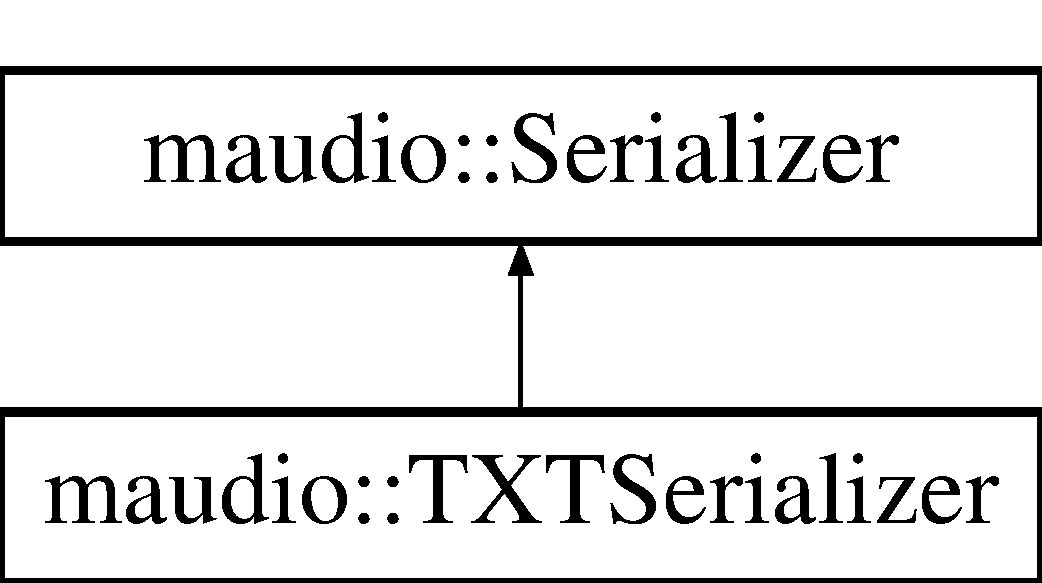
\includegraphics[height=2.000000cm]{classmaudio_1_1Serializer}
\end{center}
\end{figure}
\subsection*{Public Member Functions}
\begin{DoxyCompactItemize}
\item 
\hyperlink{classmaudio_1_1Serializer_a1586580e7306d00dde0a2ffdbcece5af}{Serializer} ()
\item 
virtual \hyperlink{classmaudio_1_1Serializer_a7501d9bdec33e283affc4e3da8da86e6}{$\sim$\-Serializer} ()
\end{DoxyCompactItemize}


\subsection{Constructor \& Destructor Documentation}
\hypertarget{classmaudio_1_1Serializer_a1586580e7306d00dde0a2ffdbcece5af}{\index{maudio\-::\-Serializer@{maudio\-::\-Serializer}!Serializer@{Serializer}}
\index{Serializer@{Serializer}!maudio::Serializer@{maudio\-::\-Serializer}}
\subsubsection[{Serializer}]{\setlength{\rightskip}{0pt plus 5cm}maudio\-::\-Serializer\-::\-Serializer (
\begin{DoxyParamCaption}
{}
\end{DoxyParamCaption}
)}}\label{classmaudio_1_1Serializer_a1586580e7306d00dde0a2ffdbcece5af}
\hypertarget{classmaudio_1_1Serializer_a7501d9bdec33e283affc4e3da8da86e6}{\index{maudio\-::\-Serializer@{maudio\-::\-Serializer}!$\sim$\-Serializer@{$\sim$\-Serializer}}
\index{$\sim$\-Serializer@{$\sim$\-Serializer}!maudio::Serializer@{maudio\-::\-Serializer}}
\subsubsection[{$\sim$\-Serializer}]{\setlength{\rightskip}{0pt plus 5cm}virtual maudio\-::\-Serializer\-::$\sim$\-Serializer (
\begin{DoxyParamCaption}
{}
\end{DoxyParamCaption}
)\hspace{0.3cm}{\ttfamily [virtual]}}}\label{classmaudio_1_1Serializer_a7501d9bdec33e283affc4e3da8da86e6}


The documentation for this class was generated from the following file\-:\begin{DoxyCompactItemize}
\item 
/home/mars/\-Projekte/maudio/src/plugins/include/core/serializer/\hyperlink{Serializer_8hpp}{Serializer.\-hpp}\end{DoxyCompactItemize}

\hypertarget{classmaudio_1_1SerializerStore}{\section{maudio\-:\-:Serializer\-Store Class Reference}
\label{classmaudio_1_1SerializerStore}\index{maudio\-::\-Serializer\-Store@{maudio\-::\-Serializer\-Store}}
}


{\ttfamily \#include $<$Serializer\-Store.\-hpp$>$}

Inheritance diagram for maudio\-:\-:Serializer\-Store\-:\begin{figure}[H]
\begin{center}
\leavevmode
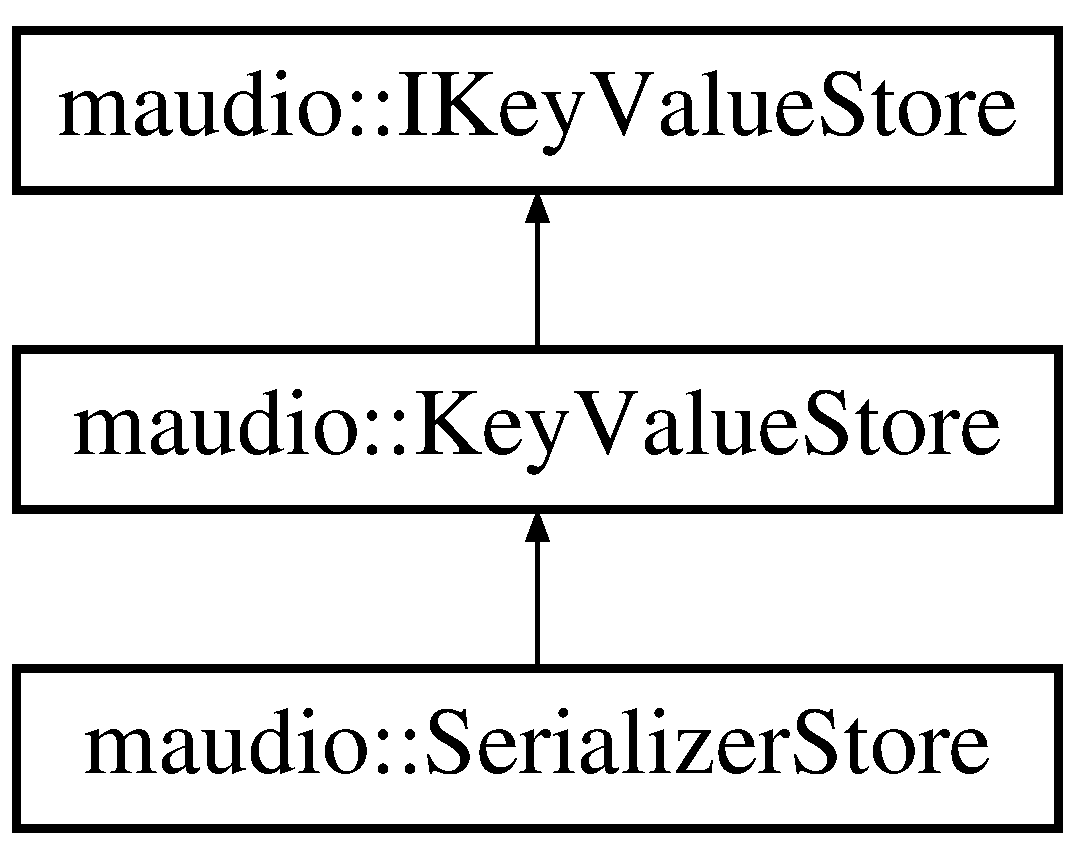
\includegraphics[height=3.000000cm]{classmaudio_1_1SerializerStore}
\end{center}
\end{figure}
\subsection*{Public Member Functions}
\begin{DoxyCompactItemize}
\item 
\hyperlink{classmaudio_1_1SerializerStore_a57e9c8cac2f585facf9c350e11b92cb8}{Serializer\-Store} ()
\item 
virtual \hyperlink{classmaudio_1_1SerializerStore_a1b821dd09fe274ccc0dc1e6a9b099a92}{$\sim$\-Serializer\-Store} ()
\end{DoxyCompactItemize}
\subsection*{Additional Inherited Members}


\subsection{Constructor \& Destructor Documentation}
\hypertarget{classmaudio_1_1SerializerStore_a57e9c8cac2f585facf9c350e11b92cb8}{\index{maudio\-::\-Serializer\-Store@{maudio\-::\-Serializer\-Store}!Serializer\-Store@{Serializer\-Store}}
\index{Serializer\-Store@{Serializer\-Store}!maudio::SerializerStore@{maudio\-::\-Serializer\-Store}}
\subsubsection[{Serializer\-Store}]{\setlength{\rightskip}{0pt plus 5cm}maudio\-::\-Serializer\-Store\-::\-Serializer\-Store (
\begin{DoxyParamCaption}
{}
\end{DoxyParamCaption}
)}}\label{classmaudio_1_1SerializerStore_a57e9c8cac2f585facf9c350e11b92cb8}
\hypertarget{classmaudio_1_1SerializerStore_a1b821dd09fe274ccc0dc1e6a9b099a92}{\index{maudio\-::\-Serializer\-Store@{maudio\-::\-Serializer\-Store}!$\sim$\-Serializer\-Store@{$\sim$\-Serializer\-Store}}
\index{$\sim$\-Serializer\-Store@{$\sim$\-Serializer\-Store}!maudio::SerializerStore@{maudio\-::\-Serializer\-Store}}
\subsubsection[{$\sim$\-Serializer\-Store}]{\setlength{\rightskip}{0pt plus 5cm}maudio\-::\-Serializer\-Store\-::$\sim$\-Serializer\-Store (
\begin{DoxyParamCaption}
{}
\end{DoxyParamCaption}
)\hspace{0.3cm}{\ttfamily [virtual]}}}\label{classmaudio_1_1SerializerStore_a1b821dd09fe274ccc0dc1e6a9b099a92}


The documentation for this class was generated from the following files\-:\begin{DoxyCompactItemize}
\item 
/home/mars/\-Projekte/maudio/src/plugins/include/core/serializer/\hyperlink{SerializerStore_8hpp}{Serializer\-Store.\-hpp}\item 
/home/mars/\-Projekte/maudio/src/core/serializer/\hyperlink{core_2serializer_2SerializerStore_8cpp}{Serializer\-Store.\-cpp}\end{DoxyCompactItemize}

\hypertarget{classmaudio_1_1simple__ptr}{\section{maudio\-:\-:simple\-\_\-ptr$<$ T $>$ Class Template Reference}
\label{classmaudio_1_1simple__ptr}\index{maudio\-::simple\-\_\-ptr$<$ T $>$@{maudio\-::simple\-\_\-ptr$<$ T $>$}}
}


{\ttfamily \#include $<$simple\-\_\-ptr.\-hpp$>$}

\subsection*{Public Member Functions}
\begin{DoxyCompactItemize}
\item 
\hyperlink{classmaudio_1_1simple__ptr_ab56e81788cacd5aa507833db4fd44bd8}{simple\-\_\-ptr} (T $\ast$data=N\-U\-L\-L)
\item 
\hyperlink{classmaudio_1_1simple__ptr_a8cba474ba00b1b94c49c707d9424b078}{simple\-\_\-ptr} (\hyperlink{classmaudio_1_1simple__ptr}{simple\-\_\-ptr}$<$ T $>$ \&data)
\item 
\hyperlink{classmaudio_1_1simple__ptr_a88310827fe1d7a361cc3fb9b787d4503}{$\sim$simple\-\_\-ptr} ()
\item 
void \hyperlink{classmaudio_1_1simple__ptr_a3eebcda59c83170bafcdab6018425501}{reset} (T $\ast$data=N\-U\-L\-L)
\item 
void \hyperlink{classmaudio_1_1simple__ptr_a6d2901d4228bfb62202a245c30eb240e}{reset} (\hyperlink{classmaudio_1_1simple__ptr}{simple\-\_\-ptr}$<$ T $>$ \&data)
\item 
T $\ast$ \hyperlink{classmaudio_1_1simple__ptr_a1a1592b302bab798fc08413a670d8807}{release} ()
\item 
T $\ast$ \hyperlink{classmaudio_1_1simple__ptr_a63b3da7d10ed480dd6a826dd6b51f76e}{get} ()
\item 
T $\ast$ \hyperlink{classmaudio_1_1simple__ptr_a4c76bf724a04025a4bd0e348f19e14c1}{operator-\/$>$} ()
\item 
T \& \hyperlink{classmaudio_1_1simple__ptr_a66f558bb874abcd373528908c9b9b985}{operator$\ast$} ()
\item 
void \hyperlink{classmaudio_1_1simple__ptr_a3eac5c9986e5550506b6a730456319d5}{operator=} (T \&data)
\item 
void \hyperlink{classmaudio_1_1simple__ptr_a19f92329a0e55c1491ada84f53983341}{operator=} (\hyperlink{classmaudio_1_1simple__ptr}{simple\-\_\-ptr}$<$ T $>$ \&data)
\item 
bool \hyperlink{classmaudio_1_1simple__ptr_aff5acc470b657ab9584f481bfe9314ec}{operator==} (\hyperlink{classmaudio_1_1simple__ptr}{simple\-\_\-ptr}$<$ T $>$ \&data)
\item 
\hyperlink{classmaudio_1_1simple__ptr_aac5cd27ca0b9e02c0d8b0945d5a66b53}{operator bool} ()
\end{DoxyCompactItemize}


\subsection{Detailed Description}
\subsubsection*{template$<$typename T$>$class maudio\-::simple\-\_\-ptr$<$ T $>$}

Takes ownership over a pointer, acts like a pointer, but deletes it when it goes out of scope. Similar to stl smart pointers but has less overhead. Best way to handle returned raw pointers. Warning\-: its not thread save! 

\subsection{Constructor \& Destructor Documentation}
\hypertarget{classmaudio_1_1simple__ptr_ab56e81788cacd5aa507833db4fd44bd8}{\index{maudio\-::simple\-\_\-ptr@{maudio\-::simple\-\_\-ptr}!simple\-\_\-ptr@{simple\-\_\-ptr}}
\index{simple\-\_\-ptr@{simple\-\_\-ptr}!maudio::simple_ptr@{maudio\-::simple\-\_\-ptr}}
\subsubsection[{simple\-\_\-ptr}]{\setlength{\rightskip}{0pt plus 5cm}template$<$typename T $>$ {\bf maudio\-::simple\-\_\-ptr}$<$ T $>$\-::{\bf simple\-\_\-ptr} (
\begin{DoxyParamCaption}
\item[{T $\ast$}]{data = {\ttfamily NULL}}
\end{DoxyParamCaption}
)}}\label{classmaudio_1_1simple__ptr_ab56e81788cacd5aa507833db4fd44bd8}
\hypertarget{classmaudio_1_1simple__ptr_a8cba474ba00b1b94c49c707d9424b078}{\index{maudio\-::simple\-\_\-ptr@{maudio\-::simple\-\_\-ptr}!simple\-\_\-ptr@{simple\-\_\-ptr}}
\index{simple\-\_\-ptr@{simple\-\_\-ptr}!maudio::simple_ptr@{maudio\-::simple\-\_\-ptr}}
\subsubsection[{simple\-\_\-ptr}]{\setlength{\rightskip}{0pt plus 5cm}template$<$typename T $>$ {\bf maudio\-::simple\-\_\-ptr}$<$ T $>$\-::{\bf simple\-\_\-ptr} (
\begin{DoxyParamCaption}
\item[{{\bf simple\-\_\-ptr}$<$ T $>$ \&}]{data}
\end{DoxyParamCaption}
)}}\label{classmaudio_1_1simple__ptr_a8cba474ba00b1b94c49c707d9424b078}
\hypertarget{classmaudio_1_1simple__ptr_a88310827fe1d7a361cc3fb9b787d4503}{\index{maudio\-::simple\-\_\-ptr@{maudio\-::simple\-\_\-ptr}!$\sim$simple\-\_\-ptr@{$\sim$simple\-\_\-ptr}}
\index{$\sim$simple\-\_\-ptr@{$\sim$simple\-\_\-ptr}!maudio::simple_ptr@{maudio\-::simple\-\_\-ptr}}
\subsubsection[{$\sim$simple\-\_\-ptr}]{\setlength{\rightskip}{0pt plus 5cm}template$<$typename T $>$ {\bf maudio\-::simple\-\_\-ptr}$<$ T $>$\-::$\sim${\bf simple\-\_\-ptr} (
\begin{DoxyParamCaption}
{}
\end{DoxyParamCaption}
)}}\label{classmaudio_1_1simple__ptr_a88310827fe1d7a361cc3fb9b787d4503}


\subsection{Member Function Documentation}
\hypertarget{classmaudio_1_1simple__ptr_a63b3da7d10ed480dd6a826dd6b51f76e}{\index{maudio\-::simple\-\_\-ptr@{maudio\-::simple\-\_\-ptr}!get@{get}}
\index{get@{get}!maudio::simple_ptr@{maudio\-::simple\-\_\-ptr}}
\subsubsection[{get}]{\setlength{\rightskip}{0pt plus 5cm}template$<$typename T $>$ T $\ast$ {\bf maudio\-::simple\-\_\-ptr}$<$ T $>$\-::get (
\begin{DoxyParamCaption}
{}
\end{DoxyParamCaption}
)}}\label{classmaudio_1_1simple__ptr_a63b3da7d10ed480dd6a826dd6b51f76e}
\hypertarget{classmaudio_1_1simple__ptr_aac5cd27ca0b9e02c0d8b0945d5a66b53}{\index{maudio\-::simple\-\_\-ptr@{maudio\-::simple\-\_\-ptr}!operator bool@{operator bool}}
\index{operator bool@{operator bool}!maudio::simple_ptr@{maudio\-::simple\-\_\-ptr}}
\subsubsection[{operator bool}]{\setlength{\rightskip}{0pt plus 5cm}template$<$typename T $>$ {\bf maudio\-::simple\-\_\-ptr}$<$ T $>$\-::operator bool (
\begin{DoxyParamCaption}
{}
\end{DoxyParamCaption}
)}}\label{classmaudio_1_1simple__ptr_aac5cd27ca0b9e02c0d8b0945d5a66b53}
\hypertarget{classmaudio_1_1simple__ptr_a66f558bb874abcd373528908c9b9b985}{\index{maudio\-::simple\-\_\-ptr@{maudio\-::simple\-\_\-ptr}!operator$\ast$@{operator$\ast$}}
\index{operator$\ast$@{operator$\ast$}!maudio::simple_ptr@{maudio\-::simple\-\_\-ptr}}
\subsubsection[{operator$\ast$}]{\setlength{\rightskip}{0pt plus 5cm}template$<$typename T $>$ T \& {\bf maudio\-::simple\-\_\-ptr}$<$ T $>$\-::operator$\ast$ (
\begin{DoxyParamCaption}
{}
\end{DoxyParamCaption}
)}}\label{classmaudio_1_1simple__ptr_a66f558bb874abcd373528908c9b9b985}
\hypertarget{classmaudio_1_1simple__ptr_a4c76bf724a04025a4bd0e348f19e14c1}{\index{maudio\-::simple\-\_\-ptr@{maudio\-::simple\-\_\-ptr}!operator-\/$>$@{operator-\/$>$}}
\index{operator-\/$>$@{operator-\/$>$}!maudio::simple_ptr@{maudio\-::simple\-\_\-ptr}}
\subsubsection[{operator-\/$>$}]{\setlength{\rightskip}{0pt plus 5cm}template$<$typename T $>$ T $\ast$ {\bf maudio\-::simple\-\_\-ptr}$<$ T $>$\-::operator-\/$>$ (
\begin{DoxyParamCaption}
{}
\end{DoxyParamCaption}
)}}\label{classmaudio_1_1simple__ptr_a4c76bf724a04025a4bd0e348f19e14c1}
\hypertarget{classmaudio_1_1simple__ptr_a3eac5c9986e5550506b6a730456319d5}{\index{maudio\-::simple\-\_\-ptr@{maudio\-::simple\-\_\-ptr}!operator=@{operator=}}
\index{operator=@{operator=}!maudio::simple_ptr@{maudio\-::simple\-\_\-ptr}}
\subsubsection[{operator=}]{\setlength{\rightskip}{0pt plus 5cm}template$<$typename T $>$ void {\bf maudio\-::simple\-\_\-ptr}$<$ T $>$\-::operator= (
\begin{DoxyParamCaption}
\item[{T \&}]{data}
\end{DoxyParamCaption}
)}}\label{classmaudio_1_1simple__ptr_a3eac5c9986e5550506b6a730456319d5}
\hypertarget{classmaudio_1_1simple__ptr_a19f92329a0e55c1491ada84f53983341}{\index{maudio\-::simple\-\_\-ptr@{maudio\-::simple\-\_\-ptr}!operator=@{operator=}}
\index{operator=@{operator=}!maudio::simple_ptr@{maudio\-::simple\-\_\-ptr}}
\subsubsection[{operator=}]{\setlength{\rightskip}{0pt plus 5cm}template$<$typename T $>$ void {\bf maudio\-::simple\-\_\-ptr}$<$ T $>$\-::operator= (
\begin{DoxyParamCaption}
\item[{{\bf simple\-\_\-ptr}$<$ T $>$ \&}]{data}
\end{DoxyParamCaption}
)}}\label{classmaudio_1_1simple__ptr_a19f92329a0e55c1491ada84f53983341}
\hypertarget{classmaudio_1_1simple__ptr_aff5acc470b657ab9584f481bfe9314ec}{\index{maudio\-::simple\-\_\-ptr@{maudio\-::simple\-\_\-ptr}!operator==@{operator==}}
\index{operator==@{operator==}!maudio::simple_ptr@{maudio\-::simple\-\_\-ptr}}
\subsubsection[{operator==}]{\setlength{\rightskip}{0pt plus 5cm}template$<$typename T $>$ bool {\bf maudio\-::simple\-\_\-ptr}$<$ T $>$\-::operator== (
\begin{DoxyParamCaption}
\item[{{\bf simple\-\_\-ptr}$<$ T $>$ \&}]{data}
\end{DoxyParamCaption}
)}}\label{classmaudio_1_1simple__ptr_aff5acc470b657ab9584f481bfe9314ec}
\hypertarget{classmaudio_1_1simple__ptr_a1a1592b302bab798fc08413a670d8807}{\index{maudio\-::simple\-\_\-ptr@{maudio\-::simple\-\_\-ptr}!release@{release}}
\index{release@{release}!maudio::simple_ptr@{maudio\-::simple\-\_\-ptr}}
\subsubsection[{release}]{\setlength{\rightskip}{0pt plus 5cm}template$<$typename T $>$ T $\ast$ {\bf maudio\-::simple\-\_\-ptr}$<$ T $>$\-::release (
\begin{DoxyParamCaption}
{}
\end{DoxyParamCaption}
)}}\label{classmaudio_1_1simple__ptr_a1a1592b302bab798fc08413a670d8807}
\hypertarget{classmaudio_1_1simple__ptr_a3eebcda59c83170bafcdab6018425501}{\index{maudio\-::simple\-\_\-ptr@{maudio\-::simple\-\_\-ptr}!reset@{reset}}
\index{reset@{reset}!maudio::simple_ptr@{maudio\-::simple\-\_\-ptr}}
\subsubsection[{reset}]{\setlength{\rightskip}{0pt plus 5cm}template$<$typename T $>$ void {\bf maudio\-::simple\-\_\-ptr}$<$ T $>$\-::reset (
\begin{DoxyParamCaption}
\item[{T $\ast$}]{data = {\ttfamily NULL}}
\end{DoxyParamCaption}
)}}\label{classmaudio_1_1simple__ptr_a3eebcda59c83170bafcdab6018425501}
\hypertarget{classmaudio_1_1simple__ptr_a6d2901d4228bfb62202a245c30eb240e}{\index{maudio\-::simple\-\_\-ptr@{maudio\-::simple\-\_\-ptr}!reset@{reset}}
\index{reset@{reset}!maudio::simple_ptr@{maudio\-::simple\-\_\-ptr}}
\subsubsection[{reset}]{\setlength{\rightskip}{0pt plus 5cm}template$<$typename T $>$ void {\bf maudio\-::simple\-\_\-ptr}$<$ T $>$\-::reset (
\begin{DoxyParamCaption}
\item[{{\bf simple\-\_\-ptr}$<$ T $>$ \&}]{data}
\end{DoxyParamCaption}
)}}\label{classmaudio_1_1simple__ptr_a6d2901d4228bfb62202a245c30eb240e}


The documentation for this class was generated from the following file\-:\begin{DoxyCompactItemize}
\item 
/home/mars/\-Projekte/maudio/src/plugins/include/core/util/\hyperlink{simple__ptr_8hpp}{simple\-\_\-ptr.\-hpp}\end{DoxyCompactItemize}

\hypertarget{classmaudio_1_1SimpleKeyableProperty}{\section{maudio\-:\-:Simple\-Keyable\-Property$<$ T $>$ Class Template Reference}
\label{classmaudio_1_1SimpleKeyableProperty}\index{maudio\-::\-Simple\-Keyable\-Property$<$ T $>$@{maudio\-::\-Simple\-Keyable\-Property$<$ T $>$}}
}


{\ttfamily \#include $<$Simple\-Keyable\-Property.\-hpp$>$}

Inheritance diagram for maudio\-:\-:Simple\-Keyable\-Property$<$ T $>$\-:\begin{figure}[H]
\begin{center}
\leavevmode
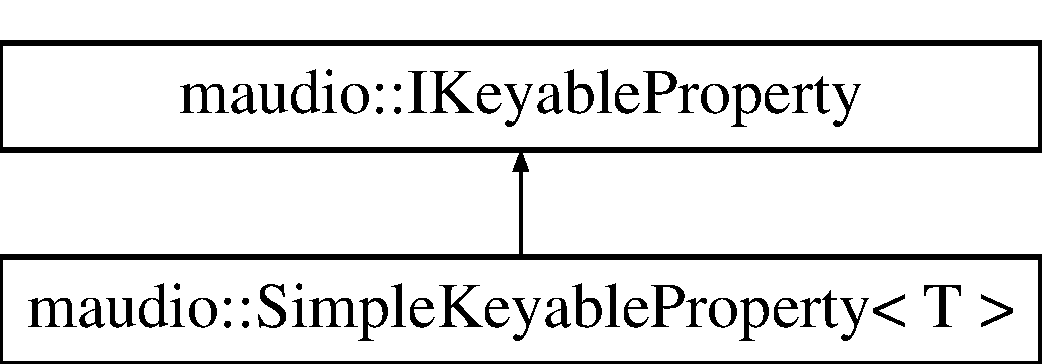
\includegraphics[height=2.000000cm]{classmaudio_1_1SimpleKeyableProperty}
\end{center}
\end{figure}
\subsection*{Public Member Functions}
\begin{DoxyCompactItemize}
\item 
\hyperlink{classmaudio_1_1SimpleKeyableProperty_a02a7f673256949d25c007a20731c248a}{Simple\-Keyable\-Property} (const char $\ast$name, T initial\-Value)
\item 
virtual \hyperlink{classmaudio_1_1SimpleKeyableProperty_ab80ec43285ef052e8922cbd5f6e2550b}{$\sim$\-Simple\-Keyable\-Property} ()
\item 
virtual const char $\ast$ \hyperlink{classmaudio_1_1SimpleKeyableProperty_ad59e0660332de7addc4d30cac06c74d6}{get\-Name} () const 
\item 
virtual const char $\ast$ \hyperlink{classmaudio_1_1SimpleKeyableProperty_ab6fcf9e2072cfeb1d2d325087b56f081}{get\-String} (long double pos) const 
\item 
virtual T \hyperlink{classmaudio_1_1SimpleKeyableProperty_a9f1d5036afe0b46da89a489c73834b91}{get} (long double pos) const 
\item 
virtual const char $\ast$ \hyperlink{classmaudio_1_1SimpleKeyableProperty_a66b1dbdffb78cd64a6ba2372aef51704}{get\-Key\-String} (unsigned int keynum) const 
\item 
virtual long double \hyperlink{classmaudio_1_1SimpleKeyableProperty_a5e7f9b7399708ed4418a97ede30ef39d}{get\-Key\-Pos} (unsigned int keynum) const 
\item 
virtual T \hyperlink{classmaudio_1_1SimpleKeyableProperty_a49b740ce101da9afd7fdaaca907fa684}{get\-Key} (unsigned int keynum) const 
\item 
virtual unsigned int \hyperlink{classmaudio_1_1SimpleKeyableProperty_a7654245fbc63b3c02623884f811e9ea8}{get\-Num\-Keys} () const 
\item 
virtual void \hyperlink{classmaudio_1_1SimpleKeyableProperty_afb3a967f864eeea050cbb3d701c5242c}{add\-Key} (const char $\ast$value, long double pos)
\item 
virtual void \hyperlink{classmaudio_1_1SimpleKeyableProperty_a1c3d5064b77c77489203d0d79f67a2c0}{add\-Key} (T value, long double pos)
\item 
virtual void \hyperlink{classmaudio_1_1SimpleKeyableProperty_a7d1cb59d08f7daf7bd68e42301f12d72}{add\-Key} (const std\-::string \&value, long double pos)
\item 
virtual void \hyperlink{classmaudio_1_1SimpleKeyableProperty_add1b65fb83c28332ed22a879949f1475}{set\-Key} (const char $\ast$value, unsigned int keynum)
\item 
virtual void \hyperlink{classmaudio_1_1SimpleKeyableProperty_a024814f5c80774c5de7c09d357b34950}{set\-Key} (T value, unsigned int keynum)
\item 
virtual void \hyperlink{classmaudio_1_1SimpleKeyableProperty_a432f634ff52d1e3eba39cfb6acda73c5}{set\-Key} (const std\-::string \&value, unsigned int keynum)
\item 
virtual void \hyperlink{classmaudio_1_1SimpleKeyableProperty_a19cb5ccd52244264ff4d53b97ebd081c}{remove\-Key} (unsigned int keynum)
\item 
virtual void \hyperlink{classmaudio_1_1SimpleKeyableProperty_a63db4ec0d5c4a289f2d20baed7587087}{set\-Bounds} (T bottom, T upper)
\item 
virtual const char $\ast$ \hyperlink{classmaudio_1_1SimpleKeyableProperty_ae3c62c7e501a8d50f1ac6220d381e7f5}{get\-Bottom\-Bounds\-String} () const 
\item 
virtual const char $\ast$ \hyperlink{classmaudio_1_1SimpleKeyableProperty_a9535fe9f61499c3b8cd79df11f7f461e}{get\-Upper\-Bounds\-String} () const 
\item 
virtual std\-::vector$<$ std\-::string $>$ \hyperlink{classmaudio_1_1SimpleKeyableProperty_a256a4b500e25f7a048d8f24280cfe893}{get\-Bounds\-String} () const 
\item 
virtual std\-::vector$<$ T $>$ \hyperlink{classmaudio_1_1SimpleKeyableProperty_a16365804a24594a466ed72ecdc3b8854}{get\-Bounds} () const 
\item 
{\footnotesize template$<$$>$ }\\const char $\ast$ \hyperlink{classmaudio_1_1SimpleKeyableProperty_a54bf26a66e66c717bc8cb3b64f830cab}{get\-String} (long double pos) const
\item 
{\footnotesize template$<$$>$ }\\const char $\ast$ \hyperlink{classmaudio_1_1SimpleKeyableProperty_a8a34984567fb8700030315bc23b1b900}{get\-Key\-String} (unsigned int keynum) const
\item 
{\footnotesize template$<$$>$ }\\const char $\ast$ \hyperlink{classmaudio_1_1SimpleKeyableProperty_ad65745f7a5dae9883621c385c87591fb}{get\-String} (long double pos) const
\item 
{\footnotesize template$<$$>$ }\\std\-::string \hyperlink{classmaudio_1_1SimpleKeyableProperty_ae7cb5d3b99c238d7d1b977c7e2a43774}{get} (long double pos) const
\item 
{\footnotesize template$<$$>$ }\\const char $\ast$ \hyperlink{classmaudio_1_1SimpleKeyableProperty_ac8459aea6d5685fa2a808ab7f13c4051}{get\-Key\-String} (unsigned int keynum) const
\item 
{\footnotesize template$<$$>$ }\\std\-::string \hyperlink{classmaudio_1_1SimpleKeyableProperty_a06900c85a334eb5770085a4758ad0711}{get\-Key} (unsigned int keynum) const
\item 
{\footnotesize template$<$$>$ }\\void \hyperlink{classmaudio_1_1SimpleKeyableProperty_aeb558a531fad8b7a997f3425be7a5b98}{add\-Key} (const std\-::string \&value, long double pos)
\item 
{\footnotesize template$<$$>$ }\\void \hyperlink{classmaudio_1_1SimpleKeyableProperty_adcc2030105e800fc71d1a25374b58554}{add\-Key} (std\-::string value, long double pos)
\item 
{\footnotesize template$<$$>$ }\\void \hyperlink{classmaudio_1_1SimpleKeyableProperty_a4031c824079fd6e619784324fa71528d}{set\-Key} (const std\-::string \&value, unsigned int keynum)
\item 
{\footnotesize template$<$$>$ }\\void \hyperlink{classmaudio_1_1SimpleKeyableProperty_a63cfcf99306b4e189556ed1f428a187c}{set\-Key} (std\-::string value, unsigned int keynum)
\item 
{\footnotesize template$<$$>$ }\\void \hyperlink{classmaudio_1_1SimpleKeyableProperty_af72906ce2cdfacbbae8cff72ae450e5a}{set\-Bounds} (std\-::string bottom, std\-::string upper)
\item 
{\footnotesize template$<$$>$ }\\std\-::vector$<$ std\-::string $>$ \hyperlink{classmaudio_1_1SimpleKeyableProperty_af442b75407c7a82f18faa1b552f2cb79}{get\-Bounds\-String} () const
\item 
{\footnotesize template$<$$>$ }\\std\-::vector$<$ std\-::string $>$ \hyperlink{classmaudio_1_1SimpleKeyableProperty_ad75a850801bc9ac0cba85ca619b8324f}{get\-Bounds} () const
\item 
{\footnotesize template$<$$>$ }\\const char $\ast$ \hyperlink{classmaudio_1_1SimpleKeyableProperty_a54bf26a66e66c717bc8cb3b64f830cab}{get\-String} (long double pos) const
\item 
{\footnotesize template$<$$>$ }\\const char $\ast$ \hyperlink{classmaudio_1_1SimpleKeyableProperty_a8a34984567fb8700030315bc23b1b900}{get\-Key\-String} (unsigned int keynum) const
\item 
{\footnotesize template$<$$>$ }\\const char $\ast$ \hyperlink{classmaudio_1_1SimpleKeyableProperty_ad65745f7a5dae9883621c385c87591fb}{get\-String} (long double pos) const
\item 
{\footnotesize template$<$$>$ }\\std\-::string \hyperlink{classmaudio_1_1SimpleKeyableProperty_ae7cb5d3b99c238d7d1b977c7e2a43774}{get} (long double pos) const
\item 
{\footnotesize template$<$$>$ }\\const char $\ast$ \hyperlink{classmaudio_1_1SimpleKeyableProperty_ac8459aea6d5685fa2a808ab7f13c4051}{get\-Key\-String} (unsigned int keynum) const
\item 
{\footnotesize template$<$$>$ }\\std\-::string \hyperlink{classmaudio_1_1SimpleKeyableProperty_a06900c85a334eb5770085a4758ad0711}{get\-Key} (unsigned int keynum) const
\item 
{\footnotesize template$<$$>$ }\\void \hyperlink{classmaudio_1_1SimpleKeyableProperty_aeb558a531fad8b7a997f3425be7a5b98}{add\-Key} (const std\-::string \&value, long double pos)
\item 
{\footnotesize template$<$$>$ }\\void \hyperlink{classmaudio_1_1SimpleKeyableProperty_adcc2030105e800fc71d1a25374b58554}{add\-Key} (std\-::string value, long double pos)
\item 
{\footnotesize template$<$$>$ }\\void \hyperlink{classmaudio_1_1SimpleKeyableProperty_a4031c824079fd6e619784324fa71528d}{set\-Key} (const std\-::string \&value, unsigned int keynum)
\item 
{\footnotesize template$<$$>$ }\\void \hyperlink{classmaudio_1_1SimpleKeyableProperty_a63cfcf99306b4e189556ed1f428a187c}{set\-Key} (std\-::string value, unsigned int keynum)
\item 
{\footnotesize template$<$$>$ }\\void \hyperlink{classmaudio_1_1SimpleKeyableProperty_af72906ce2cdfacbbae8cff72ae450e5a}{set\-Bounds} (std\-::string bottom, std\-::string upper)
\item 
{\footnotesize template$<$$>$ }\\std\-::vector$<$ std\-::string $>$ \hyperlink{classmaudio_1_1SimpleKeyableProperty_af442b75407c7a82f18faa1b552f2cb79}{get\-Bounds\-String} () const
\item 
{\footnotesize template$<$$>$ }\\std\-::vector$<$ std\-::string $>$ \hyperlink{classmaudio_1_1SimpleKeyableProperty_ad75a850801bc9ac0cba85ca619b8324f}{get\-Bounds} () const
\end{DoxyCompactItemize}


\subsection{Constructor \& Destructor Documentation}
\hypertarget{classmaudio_1_1SimpleKeyableProperty_a02a7f673256949d25c007a20731c248a}{\index{maudio\-::\-Simple\-Keyable\-Property@{maudio\-::\-Simple\-Keyable\-Property}!Simple\-Keyable\-Property@{Simple\-Keyable\-Property}}
\index{Simple\-Keyable\-Property@{Simple\-Keyable\-Property}!maudio::SimpleKeyableProperty@{maudio\-::\-Simple\-Keyable\-Property}}
\subsubsection[{Simple\-Keyable\-Property}]{\setlength{\rightskip}{0pt plus 5cm}template$<$typename T $>$ {\bf maudio\-::\-Simple\-Keyable\-Property}$<$ T $>$\-::{\bf Simple\-Keyable\-Property} (
\begin{DoxyParamCaption}
\item[{const char $\ast$}]{name, }
\item[{T}]{initial\-Value}
\end{DoxyParamCaption}
)}}\label{classmaudio_1_1SimpleKeyableProperty_a02a7f673256949d25c007a20731c248a}
\hypertarget{classmaudio_1_1SimpleKeyableProperty_ab80ec43285ef052e8922cbd5f6e2550b}{\index{maudio\-::\-Simple\-Keyable\-Property@{maudio\-::\-Simple\-Keyable\-Property}!$\sim$\-Simple\-Keyable\-Property@{$\sim$\-Simple\-Keyable\-Property}}
\index{$\sim$\-Simple\-Keyable\-Property@{$\sim$\-Simple\-Keyable\-Property}!maudio::SimpleKeyableProperty@{maudio\-::\-Simple\-Keyable\-Property}}
\subsubsection[{$\sim$\-Simple\-Keyable\-Property}]{\setlength{\rightskip}{0pt plus 5cm}template$<$typename T $>$ {\bf maudio\-::\-Simple\-Keyable\-Property}$<$ T $>$\-::$\sim${\bf Simple\-Keyable\-Property} (
\begin{DoxyParamCaption}
{}
\end{DoxyParamCaption}
)\hspace{0.3cm}{\ttfamily [virtual]}}}\label{classmaudio_1_1SimpleKeyableProperty_ab80ec43285ef052e8922cbd5f6e2550b}


\subsection{Member Function Documentation}
\hypertarget{classmaudio_1_1SimpleKeyableProperty_afb3a967f864eeea050cbb3d701c5242c}{\index{maudio\-::\-Simple\-Keyable\-Property@{maudio\-::\-Simple\-Keyable\-Property}!add\-Key@{add\-Key}}
\index{add\-Key@{add\-Key}!maudio::SimpleKeyableProperty@{maudio\-::\-Simple\-Keyable\-Property}}
\subsubsection[{add\-Key}]{\setlength{\rightskip}{0pt plus 5cm}template$<$typename T $>$ void {\bf maudio\-::\-Simple\-Keyable\-Property}$<$ T $>$\-::add\-Key (
\begin{DoxyParamCaption}
\item[{const char $\ast$}]{value, }
\item[{long double}]{pos}
\end{DoxyParamCaption}
)\hspace{0.3cm}{\ttfamily [virtual]}}}\label{classmaudio_1_1SimpleKeyableProperty_afb3a967f864eeea050cbb3d701c5242c}


Implements \hyperlink{classmaudio_1_1IKeyableProperty_abdfffe5b0cdd27083714826014d2dfd9}{maudio\-::\-I\-Keyable\-Property}.

\hypertarget{classmaudio_1_1SimpleKeyableProperty_a1c3d5064b77c77489203d0d79f67a2c0}{\index{maudio\-::\-Simple\-Keyable\-Property@{maudio\-::\-Simple\-Keyable\-Property}!add\-Key@{add\-Key}}
\index{add\-Key@{add\-Key}!maudio::SimpleKeyableProperty@{maudio\-::\-Simple\-Keyable\-Property}}
\subsubsection[{add\-Key}]{\setlength{\rightskip}{0pt plus 5cm}template$<$typename T $>$ void {\bf maudio\-::\-Simple\-Keyable\-Property}$<$ T $>$\-::add\-Key (
\begin{DoxyParamCaption}
\item[{T}]{value, }
\item[{long double}]{pos}
\end{DoxyParamCaption}
)\hspace{0.3cm}{\ttfamily [virtual]}}}\label{classmaudio_1_1SimpleKeyableProperty_a1c3d5064b77c77489203d0d79f67a2c0}
\hypertarget{classmaudio_1_1SimpleKeyableProperty_a7d1cb59d08f7daf7bd68e42301f12d72}{\index{maudio\-::\-Simple\-Keyable\-Property@{maudio\-::\-Simple\-Keyable\-Property}!add\-Key@{add\-Key}}
\index{add\-Key@{add\-Key}!maudio::SimpleKeyableProperty@{maudio\-::\-Simple\-Keyable\-Property}}
\subsubsection[{add\-Key}]{\setlength{\rightskip}{0pt plus 5cm}template$<$typename T $>$ void {\bf maudio\-::\-Simple\-Keyable\-Property}$<$ T $>$\-::add\-Key (
\begin{DoxyParamCaption}
\item[{const std\-::string \&}]{value, }
\item[{long double}]{pos}
\end{DoxyParamCaption}
)\hspace{0.3cm}{\ttfamily [virtual]}}}\label{classmaudio_1_1SimpleKeyableProperty_a7d1cb59d08f7daf7bd68e42301f12d72}
\hypertarget{classmaudio_1_1SimpleKeyableProperty_aeb558a531fad8b7a997f3425be7a5b98}{\index{maudio\-::\-Simple\-Keyable\-Property@{maudio\-::\-Simple\-Keyable\-Property}!add\-Key@{add\-Key}}
\index{add\-Key@{add\-Key}!maudio::SimpleKeyableProperty@{maudio\-::\-Simple\-Keyable\-Property}}
\subsubsection[{add\-Key}]{\setlength{\rightskip}{0pt plus 5cm}template$<$$>$ void {\bf maudio\-::\-Simple\-Keyable\-Property}$<$ std\-::string $>$\-::add\-Key (
\begin{DoxyParamCaption}
\item[{const std\-::string \&}]{value, }
\item[{long double}]{pos}
\end{DoxyParamCaption}
)}}\label{classmaudio_1_1SimpleKeyableProperty_aeb558a531fad8b7a997f3425be7a5b98}
\hypertarget{classmaudio_1_1SimpleKeyableProperty_aeb558a531fad8b7a997f3425be7a5b98}{\index{maudio\-::\-Simple\-Keyable\-Property@{maudio\-::\-Simple\-Keyable\-Property}!add\-Key@{add\-Key}}
\index{add\-Key@{add\-Key}!maudio::SimpleKeyableProperty@{maudio\-::\-Simple\-Keyable\-Property}}
\subsubsection[{add\-Key}]{\setlength{\rightskip}{0pt plus 5cm}template$<$$>$ void {\bf maudio\-::\-Simple\-Keyable\-Property}$<$ std\-::string $>$\-::add\-Key (
\begin{DoxyParamCaption}
\item[{const std\-::string \&}]{value, }
\item[{long double}]{pos}
\end{DoxyParamCaption}
)}}\label{classmaudio_1_1SimpleKeyableProperty_aeb558a531fad8b7a997f3425be7a5b98}
\hypertarget{classmaudio_1_1SimpleKeyableProperty_adcc2030105e800fc71d1a25374b58554}{\index{maudio\-::\-Simple\-Keyable\-Property@{maudio\-::\-Simple\-Keyable\-Property}!add\-Key@{add\-Key}}
\index{add\-Key@{add\-Key}!maudio::SimpleKeyableProperty@{maudio\-::\-Simple\-Keyable\-Property}}
\subsubsection[{add\-Key}]{\setlength{\rightskip}{0pt plus 5cm}template$<$$>$ void {\bf maudio\-::\-Simple\-Keyable\-Property}$<$ std\-::string $>$\-::add\-Key (
\begin{DoxyParamCaption}
\item[{std\-::string}]{value, }
\item[{long double}]{pos}
\end{DoxyParamCaption}
)}}\label{classmaudio_1_1SimpleKeyableProperty_adcc2030105e800fc71d1a25374b58554}
\hypertarget{classmaudio_1_1SimpleKeyableProperty_adcc2030105e800fc71d1a25374b58554}{\index{maudio\-::\-Simple\-Keyable\-Property@{maudio\-::\-Simple\-Keyable\-Property}!add\-Key@{add\-Key}}
\index{add\-Key@{add\-Key}!maudio::SimpleKeyableProperty@{maudio\-::\-Simple\-Keyable\-Property}}
\subsubsection[{add\-Key}]{\setlength{\rightskip}{0pt plus 5cm}template$<$$>$ void {\bf maudio\-::\-Simple\-Keyable\-Property}$<$ std\-::string $>$\-::add\-Key (
\begin{DoxyParamCaption}
\item[{std\-::string}]{value, }
\item[{long double}]{pos}
\end{DoxyParamCaption}
)}}\label{classmaudio_1_1SimpleKeyableProperty_adcc2030105e800fc71d1a25374b58554}
\hypertarget{classmaudio_1_1SimpleKeyableProperty_a9f1d5036afe0b46da89a489c73834b91}{\index{maudio\-::\-Simple\-Keyable\-Property@{maudio\-::\-Simple\-Keyable\-Property}!get@{get}}
\index{get@{get}!maudio::SimpleKeyableProperty@{maudio\-::\-Simple\-Keyable\-Property}}
\subsubsection[{get}]{\setlength{\rightskip}{0pt plus 5cm}template$<$typename T $>$ T {\bf maudio\-::\-Simple\-Keyable\-Property}$<$ T $>$\-::get (
\begin{DoxyParamCaption}
\item[{long double}]{pos}
\end{DoxyParamCaption}
) const\hspace{0.3cm}{\ttfamily [virtual]}}}\label{classmaudio_1_1SimpleKeyableProperty_a9f1d5036afe0b46da89a489c73834b91}
\hypertarget{classmaudio_1_1SimpleKeyableProperty_ae7cb5d3b99c238d7d1b977c7e2a43774}{\index{maudio\-::\-Simple\-Keyable\-Property@{maudio\-::\-Simple\-Keyable\-Property}!get@{get}}
\index{get@{get}!maudio::SimpleKeyableProperty@{maudio\-::\-Simple\-Keyable\-Property}}
\subsubsection[{get}]{\setlength{\rightskip}{0pt plus 5cm}template$<$$>$ std\-::string {\bf maudio\-::\-Simple\-Keyable\-Property}$<$ std\-::string $>$\-::get (
\begin{DoxyParamCaption}
\item[{long double}]{pos}
\end{DoxyParamCaption}
) const}}\label{classmaudio_1_1SimpleKeyableProperty_ae7cb5d3b99c238d7d1b977c7e2a43774}
\hypertarget{classmaudio_1_1SimpleKeyableProperty_ae7cb5d3b99c238d7d1b977c7e2a43774}{\index{maudio\-::\-Simple\-Keyable\-Property@{maudio\-::\-Simple\-Keyable\-Property}!get@{get}}
\index{get@{get}!maudio::SimpleKeyableProperty@{maudio\-::\-Simple\-Keyable\-Property}}
\subsubsection[{get}]{\setlength{\rightskip}{0pt plus 5cm}template$<$$>$ std\-::string {\bf maudio\-::\-Simple\-Keyable\-Property}$<$ std\-::string $>$\-::get (
\begin{DoxyParamCaption}
\item[{long double}]{pos}
\end{DoxyParamCaption}
) const}}\label{classmaudio_1_1SimpleKeyableProperty_ae7cb5d3b99c238d7d1b977c7e2a43774}
\hypertarget{classmaudio_1_1SimpleKeyableProperty_ae3c62c7e501a8d50f1ac6220d381e7f5}{\index{maudio\-::\-Simple\-Keyable\-Property@{maudio\-::\-Simple\-Keyable\-Property}!get\-Bottom\-Bounds\-String@{get\-Bottom\-Bounds\-String}}
\index{get\-Bottom\-Bounds\-String@{get\-Bottom\-Bounds\-String}!maudio::SimpleKeyableProperty@{maudio\-::\-Simple\-Keyable\-Property}}
\subsubsection[{get\-Bottom\-Bounds\-String}]{\setlength{\rightskip}{0pt plus 5cm}template$<$typename T $>$ const char $\ast$ {\bf maudio\-::\-Simple\-Keyable\-Property}$<$ T $>$\-::get\-Bottom\-Bounds\-String (
\begin{DoxyParamCaption}
{}
\end{DoxyParamCaption}
) const\hspace{0.3cm}{\ttfamily [virtual]}}}\label{classmaudio_1_1SimpleKeyableProperty_ae3c62c7e501a8d50f1ac6220d381e7f5}


Implements \hyperlink{classmaudio_1_1IKeyableProperty_aca107fbec3117a448c48c2cf4f226198}{maudio\-::\-I\-Keyable\-Property}.

\hypertarget{classmaudio_1_1SimpleKeyableProperty_a16365804a24594a466ed72ecdc3b8854}{\index{maudio\-::\-Simple\-Keyable\-Property@{maudio\-::\-Simple\-Keyable\-Property}!get\-Bounds@{get\-Bounds}}
\index{get\-Bounds@{get\-Bounds}!maudio::SimpleKeyableProperty@{maudio\-::\-Simple\-Keyable\-Property}}
\subsubsection[{get\-Bounds}]{\setlength{\rightskip}{0pt plus 5cm}template$<$typename T $>$ std\-::vector$<$ T $>$ {\bf maudio\-::\-Simple\-Keyable\-Property}$<$ T $>$\-::get\-Bounds (
\begin{DoxyParamCaption}
{}
\end{DoxyParamCaption}
) const\hspace{0.3cm}{\ttfamily [virtual]}}}\label{classmaudio_1_1SimpleKeyableProperty_a16365804a24594a466ed72ecdc3b8854}
\hypertarget{classmaudio_1_1SimpleKeyableProperty_ad75a850801bc9ac0cba85ca619b8324f}{\index{maudio\-::\-Simple\-Keyable\-Property@{maudio\-::\-Simple\-Keyable\-Property}!get\-Bounds@{get\-Bounds}}
\index{get\-Bounds@{get\-Bounds}!maudio::SimpleKeyableProperty@{maudio\-::\-Simple\-Keyable\-Property}}
\subsubsection[{get\-Bounds}]{\setlength{\rightskip}{0pt plus 5cm}template$<$$>$ std\-::vector$<$ std\-::string $>$ {\bf maudio\-::\-Simple\-Keyable\-Property}$<$ std\-::string $>$\-::get\-Bounds (
\begin{DoxyParamCaption}
{}
\end{DoxyParamCaption}
) const}}\label{classmaudio_1_1SimpleKeyableProperty_ad75a850801bc9ac0cba85ca619b8324f}
\hypertarget{classmaudio_1_1SimpleKeyableProperty_ad75a850801bc9ac0cba85ca619b8324f}{\index{maudio\-::\-Simple\-Keyable\-Property@{maudio\-::\-Simple\-Keyable\-Property}!get\-Bounds@{get\-Bounds}}
\index{get\-Bounds@{get\-Bounds}!maudio::SimpleKeyableProperty@{maudio\-::\-Simple\-Keyable\-Property}}
\subsubsection[{get\-Bounds}]{\setlength{\rightskip}{0pt plus 5cm}template$<$$>$ std\-::vector$<$ std\-::string $>$ {\bf maudio\-::\-Simple\-Keyable\-Property}$<$ std\-::string $>$\-::get\-Bounds (
\begin{DoxyParamCaption}
{}
\end{DoxyParamCaption}
) const}}\label{classmaudio_1_1SimpleKeyableProperty_ad75a850801bc9ac0cba85ca619b8324f}
\hypertarget{classmaudio_1_1SimpleKeyableProperty_a256a4b500e25f7a048d8f24280cfe893}{\index{maudio\-::\-Simple\-Keyable\-Property@{maudio\-::\-Simple\-Keyable\-Property}!get\-Bounds\-String@{get\-Bounds\-String}}
\index{get\-Bounds\-String@{get\-Bounds\-String}!maudio::SimpleKeyableProperty@{maudio\-::\-Simple\-Keyable\-Property}}
\subsubsection[{get\-Bounds\-String}]{\setlength{\rightskip}{0pt plus 5cm}template$<$typename T $>$ std\-::vector$<$ std\-::string $>$ {\bf maudio\-::\-Simple\-Keyable\-Property}$<$ T $>$\-::get\-Bounds\-String (
\begin{DoxyParamCaption}
{}
\end{DoxyParamCaption}
) const\hspace{0.3cm}{\ttfamily [virtual]}}}\label{classmaudio_1_1SimpleKeyableProperty_a256a4b500e25f7a048d8f24280cfe893}
\hypertarget{classmaudio_1_1SimpleKeyableProperty_af442b75407c7a82f18faa1b552f2cb79}{\index{maudio\-::\-Simple\-Keyable\-Property@{maudio\-::\-Simple\-Keyable\-Property}!get\-Bounds\-String@{get\-Bounds\-String}}
\index{get\-Bounds\-String@{get\-Bounds\-String}!maudio::SimpleKeyableProperty@{maudio\-::\-Simple\-Keyable\-Property}}
\subsubsection[{get\-Bounds\-String}]{\setlength{\rightskip}{0pt plus 5cm}template$<$$>$ std\-::vector$<$ std\-::string $>$ {\bf maudio\-::\-Simple\-Keyable\-Property}$<$ std\-::string $>$\-::get\-Bounds\-String (
\begin{DoxyParamCaption}
{}
\end{DoxyParamCaption}
) const}}\label{classmaudio_1_1SimpleKeyableProperty_af442b75407c7a82f18faa1b552f2cb79}
\hypertarget{classmaudio_1_1SimpleKeyableProperty_af442b75407c7a82f18faa1b552f2cb79}{\index{maudio\-::\-Simple\-Keyable\-Property@{maudio\-::\-Simple\-Keyable\-Property}!get\-Bounds\-String@{get\-Bounds\-String}}
\index{get\-Bounds\-String@{get\-Bounds\-String}!maudio::SimpleKeyableProperty@{maudio\-::\-Simple\-Keyable\-Property}}
\subsubsection[{get\-Bounds\-String}]{\setlength{\rightskip}{0pt plus 5cm}template$<$$>$ std\-::vector$<$ std\-::string $>$ {\bf maudio\-::\-Simple\-Keyable\-Property}$<$ std\-::string $>$\-::get\-Bounds\-String (
\begin{DoxyParamCaption}
{}
\end{DoxyParamCaption}
) const}}\label{classmaudio_1_1SimpleKeyableProperty_af442b75407c7a82f18faa1b552f2cb79}
\hypertarget{classmaudio_1_1SimpleKeyableProperty_a49b740ce101da9afd7fdaaca907fa684}{\index{maudio\-::\-Simple\-Keyable\-Property@{maudio\-::\-Simple\-Keyable\-Property}!get\-Key@{get\-Key}}
\index{get\-Key@{get\-Key}!maudio::SimpleKeyableProperty@{maudio\-::\-Simple\-Keyable\-Property}}
\subsubsection[{get\-Key}]{\setlength{\rightskip}{0pt plus 5cm}template$<$typename T $>$ T {\bf maudio\-::\-Simple\-Keyable\-Property}$<$ T $>$\-::get\-Key (
\begin{DoxyParamCaption}
\item[{unsigned int}]{keynum}
\end{DoxyParamCaption}
) const\hspace{0.3cm}{\ttfamily [virtual]}}}\label{classmaudio_1_1SimpleKeyableProperty_a49b740ce101da9afd7fdaaca907fa684}
\hypertarget{classmaudio_1_1SimpleKeyableProperty_a06900c85a334eb5770085a4758ad0711}{\index{maudio\-::\-Simple\-Keyable\-Property@{maudio\-::\-Simple\-Keyable\-Property}!get\-Key@{get\-Key}}
\index{get\-Key@{get\-Key}!maudio::SimpleKeyableProperty@{maudio\-::\-Simple\-Keyable\-Property}}
\subsubsection[{get\-Key}]{\setlength{\rightskip}{0pt plus 5cm}template$<$$>$ std\-::string {\bf maudio\-::\-Simple\-Keyable\-Property}$<$ std\-::string $>$\-::get\-Key (
\begin{DoxyParamCaption}
\item[{unsigned int}]{keynum}
\end{DoxyParamCaption}
) const}}\label{classmaudio_1_1SimpleKeyableProperty_a06900c85a334eb5770085a4758ad0711}
\hypertarget{classmaudio_1_1SimpleKeyableProperty_a06900c85a334eb5770085a4758ad0711}{\index{maudio\-::\-Simple\-Keyable\-Property@{maudio\-::\-Simple\-Keyable\-Property}!get\-Key@{get\-Key}}
\index{get\-Key@{get\-Key}!maudio::SimpleKeyableProperty@{maudio\-::\-Simple\-Keyable\-Property}}
\subsubsection[{get\-Key}]{\setlength{\rightskip}{0pt plus 5cm}template$<$$>$ std\-::string {\bf maudio\-::\-Simple\-Keyable\-Property}$<$ std\-::string $>$\-::get\-Key (
\begin{DoxyParamCaption}
\item[{unsigned int}]{keynum}
\end{DoxyParamCaption}
) const}}\label{classmaudio_1_1SimpleKeyableProperty_a06900c85a334eb5770085a4758ad0711}
\hypertarget{classmaudio_1_1SimpleKeyableProperty_a5e7f9b7399708ed4418a97ede30ef39d}{\index{maudio\-::\-Simple\-Keyable\-Property@{maudio\-::\-Simple\-Keyable\-Property}!get\-Key\-Pos@{get\-Key\-Pos}}
\index{get\-Key\-Pos@{get\-Key\-Pos}!maudio::SimpleKeyableProperty@{maudio\-::\-Simple\-Keyable\-Property}}
\subsubsection[{get\-Key\-Pos}]{\setlength{\rightskip}{0pt plus 5cm}template$<$typename T $>$ long double {\bf maudio\-::\-Simple\-Keyable\-Property}$<$ T $>$\-::get\-Key\-Pos (
\begin{DoxyParamCaption}
\item[{unsigned int}]{keynum}
\end{DoxyParamCaption}
) const\hspace{0.3cm}{\ttfamily [virtual]}}}\label{classmaudio_1_1SimpleKeyableProperty_a5e7f9b7399708ed4418a97ede30ef39d}


Implements \hyperlink{classmaudio_1_1IKeyableProperty_a6412f2574d0ca4948b81ba62efd695c3}{maudio\-::\-I\-Keyable\-Property}.

\hypertarget{classmaudio_1_1SimpleKeyableProperty_a8a34984567fb8700030315bc23b1b900}{\index{maudio\-::\-Simple\-Keyable\-Property@{maudio\-::\-Simple\-Keyable\-Property}!get\-Key\-String@{get\-Key\-String}}
\index{get\-Key\-String@{get\-Key\-String}!maudio::SimpleKeyableProperty@{maudio\-::\-Simple\-Keyable\-Property}}
\subsubsection[{get\-Key\-String}]{\setlength{\rightskip}{0pt plus 5cm}template$<$$>$ const char $\ast$ {\bf maudio\-::\-Simple\-Keyable\-Property}$<$ bool $>$\-::get\-Key\-String (
\begin{DoxyParamCaption}
\item[{unsigned int}]{keynum}
\end{DoxyParamCaption}
) const\hspace{0.3cm}{\ttfamily [virtual]}}}\label{classmaudio_1_1SimpleKeyableProperty_a8a34984567fb8700030315bc23b1b900}


Implements \hyperlink{classmaudio_1_1IKeyableProperty_a219e9bbe5f66145aeb5d7449e0598220}{maudio\-::\-I\-Keyable\-Property}.

\hypertarget{classmaudio_1_1SimpleKeyableProperty_a66b1dbdffb78cd64a6ba2372aef51704}{\index{maudio\-::\-Simple\-Keyable\-Property@{maudio\-::\-Simple\-Keyable\-Property}!get\-Key\-String@{get\-Key\-String}}
\index{get\-Key\-String@{get\-Key\-String}!maudio::SimpleKeyableProperty@{maudio\-::\-Simple\-Keyable\-Property}}
\subsubsection[{get\-Key\-String}]{\setlength{\rightskip}{0pt plus 5cm}template$<$typename T $>$ const char $\ast$ {\bf maudio\-::\-Simple\-Keyable\-Property}$<$ T $>$\-::get\-Key\-String (
\begin{DoxyParamCaption}
\item[{unsigned int}]{keynum}
\end{DoxyParamCaption}
) const\hspace{0.3cm}{\ttfamily [virtual]}}}\label{classmaudio_1_1SimpleKeyableProperty_a66b1dbdffb78cd64a6ba2372aef51704}


Implements \hyperlink{classmaudio_1_1IKeyableProperty_a219e9bbe5f66145aeb5d7449e0598220}{maudio\-::\-I\-Keyable\-Property}.

\hypertarget{classmaudio_1_1SimpleKeyableProperty_a8a34984567fb8700030315bc23b1b900}{\index{maudio\-::\-Simple\-Keyable\-Property@{maudio\-::\-Simple\-Keyable\-Property}!get\-Key\-String@{get\-Key\-String}}
\index{get\-Key\-String@{get\-Key\-String}!maudio::SimpleKeyableProperty@{maudio\-::\-Simple\-Keyable\-Property}}
\subsubsection[{get\-Key\-String}]{\setlength{\rightskip}{0pt plus 5cm}template$<$$>$ const char $\ast$ {\bf maudio\-::\-Simple\-Keyable\-Property}$<$ bool $>$\-::get\-Key\-String (
\begin{DoxyParamCaption}
\item[{unsigned int}]{keynum}
\end{DoxyParamCaption}
) const\hspace{0.3cm}{\ttfamily [virtual]}}}\label{classmaudio_1_1SimpleKeyableProperty_a8a34984567fb8700030315bc23b1b900}


Implements \hyperlink{classmaudio_1_1IKeyableProperty_a219e9bbe5f66145aeb5d7449e0598220}{maudio\-::\-I\-Keyable\-Property}.

\hypertarget{classmaudio_1_1SimpleKeyableProperty_ac8459aea6d5685fa2a808ab7f13c4051}{\index{maudio\-::\-Simple\-Keyable\-Property@{maudio\-::\-Simple\-Keyable\-Property}!get\-Key\-String@{get\-Key\-String}}
\index{get\-Key\-String@{get\-Key\-String}!maudio::SimpleKeyableProperty@{maudio\-::\-Simple\-Keyable\-Property}}
\subsubsection[{get\-Key\-String}]{\setlength{\rightskip}{0pt plus 5cm}template$<$$>$ const char $\ast$ {\bf maudio\-::\-Simple\-Keyable\-Property}$<$ std\-::string $>$\-::get\-Key\-String (
\begin{DoxyParamCaption}
\item[{unsigned int}]{keynum}
\end{DoxyParamCaption}
) const\hspace{0.3cm}{\ttfamily [virtual]}}}\label{classmaudio_1_1SimpleKeyableProperty_ac8459aea6d5685fa2a808ab7f13c4051}


Implements \hyperlink{classmaudio_1_1IKeyableProperty_a219e9bbe5f66145aeb5d7449e0598220}{maudio\-::\-I\-Keyable\-Property}.

\hypertarget{classmaudio_1_1SimpleKeyableProperty_ac8459aea6d5685fa2a808ab7f13c4051}{\index{maudio\-::\-Simple\-Keyable\-Property@{maudio\-::\-Simple\-Keyable\-Property}!get\-Key\-String@{get\-Key\-String}}
\index{get\-Key\-String@{get\-Key\-String}!maudio::SimpleKeyableProperty@{maudio\-::\-Simple\-Keyable\-Property}}
\subsubsection[{get\-Key\-String}]{\setlength{\rightskip}{0pt plus 5cm}template$<$$>$ const char $\ast$ {\bf maudio\-::\-Simple\-Keyable\-Property}$<$ std\-::string $>$\-::get\-Key\-String (
\begin{DoxyParamCaption}
\item[{unsigned int}]{keynum}
\end{DoxyParamCaption}
) const\hspace{0.3cm}{\ttfamily [virtual]}}}\label{classmaudio_1_1SimpleKeyableProperty_ac8459aea6d5685fa2a808ab7f13c4051}


Implements \hyperlink{classmaudio_1_1IKeyableProperty_a219e9bbe5f66145aeb5d7449e0598220}{maudio\-::\-I\-Keyable\-Property}.

\hypertarget{classmaudio_1_1SimpleKeyableProperty_ad59e0660332de7addc4d30cac06c74d6}{\index{maudio\-::\-Simple\-Keyable\-Property@{maudio\-::\-Simple\-Keyable\-Property}!get\-Name@{get\-Name}}
\index{get\-Name@{get\-Name}!maudio::SimpleKeyableProperty@{maudio\-::\-Simple\-Keyable\-Property}}
\subsubsection[{get\-Name}]{\setlength{\rightskip}{0pt plus 5cm}template$<$typename T $>$ const char $\ast$ {\bf maudio\-::\-Simple\-Keyable\-Property}$<$ T $>$\-::get\-Name (
\begin{DoxyParamCaption}
{}
\end{DoxyParamCaption}
) const\hspace{0.3cm}{\ttfamily [virtual]}}}\label{classmaudio_1_1SimpleKeyableProperty_ad59e0660332de7addc4d30cac06c74d6}


Implements \hyperlink{classmaudio_1_1IKeyableProperty_a7f216d19b9074b2bda72b54e1c3034ea}{maudio\-::\-I\-Keyable\-Property}.

\hypertarget{classmaudio_1_1SimpleKeyableProperty_a7654245fbc63b3c02623884f811e9ea8}{\index{maudio\-::\-Simple\-Keyable\-Property@{maudio\-::\-Simple\-Keyable\-Property}!get\-Num\-Keys@{get\-Num\-Keys}}
\index{get\-Num\-Keys@{get\-Num\-Keys}!maudio::SimpleKeyableProperty@{maudio\-::\-Simple\-Keyable\-Property}}
\subsubsection[{get\-Num\-Keys}]{\setlength{\rightskip}{0pt plus 5cm}template$<$typename T $>$ unsigned int {\bf maudio\-::\-Simple\-Keyable\-Property}$<$ T $>$\-::get\-Num\-Keys (
\begin{DoxyParamCaption}
{}
\end{DoxyParamCaption}
) const\hspace{0.3cm}{\ttfamily [virtual]}}}\label{classmaudio_1_1SimpleKeyableProperty_a7654245fbc63b3c02623884f811e9ea8}


Implements \hyperlink{classmaudio_1_1IKeyableProperty_a471a706e69c4c42679fd2e3bd40dee5f}{maudio\-::\-I\-Keyable\-Property}.

\hypertarget{classmaudio_1_1SimpleKeyableProperty_a54bf26a66e66c717bc8cb3b64f830cab}{\index{maudio\-::\-Simple\-Keyable\-Property@{maudio\-::\-Simple\-Keyable\-Property}!get\-String@{get\-String}}
\index{get\-String@{get\-String}!maudio::SimpleKeyableProperty@{maudio\-::\-Simple\-Keyable\-Property}}
\subsubsection[{get\-String}]{\setlength{\rightskip}{0pt plus 5cm}template$<$$>$ const char $\ast$ {\bf maudio\-::\-Simple\-Keyable\-Property}$<$ bool $>$\-::get\-String (
\begin{DoxyParamCaption}
\item[{long double}]{pos}
\end{DoxyParamCaption}
) const\hspace{0.3cm}{\ttfamily [virtual]}}}\label{classmaudio_1_1SimpleKeyableProperty_a54bf26a66e66c717bc8cb3b64f830cab}


Implements \hyperlink{classmaudio_1_1IKeyableProperty_af28a9b9fb457b638624257cdfb2fbeef}{maudio\-::\-I\-Keyable\-Property}.

\hypertarget{classmaudio_1_1SimpleKeyableProperty_a54bf26a66e66c717bc8cb3b64f830cab}{\index{maudio\-::\-Simple\-Keyable\-Property@{maudio\-::\-Simple\-Keyable\-Property}!get\-String@{get\-String}}
\index{get\-String@{get\-String}!maudio::SimpleKeyableProperty@{maudio\-::\-Simple\-Keyable\-Property}}
\subsubsection[{get\-String}]{\setlength{\rightskip}{0pt plus 5cm}template$<$$>$ const char $\ast$ {\bf maudio\-::\-Simple\-Keyable\-Property}$<$ bool $>$\-::get\-String (
\begin{DoxyParamCaption}
\item[{long double}]{pos}
\end{DoxyParamCaption}
) const\hspace{0.3cm}{\ttfamily [virtual]}}}\label{classmaudio_1_1SimpleKeyableProperty_a54bf26a66e66c717bc8cb3b64f830cab}


Implements \hyperlink{classmaudio_1_1IKeyableProperty_af28a9b9fb457b638624257cdfb2fbeef}{maudio\-::\-I\-Keyable\-Property}.

\hypertarget{classmaudio_1_1SimpleKeyableProperty_ab6fcf9e2072cfeb1d2d325087b56f081}{\index{maudio\-::\-Simple\-Keyable\-Property@{maudio\-::\-Simple\-Keyable\-Property}!get\-String@{get\-String}}
\index{get\-String@{get\-String}!maudio::SimpleKeyableProperty@{maudio\-::\-Simple\-Keyable\-Property}}
\subsubsection[{get\-String}]{\setlength{\rightskip}{0pt plus 5cm}template$<$typename T $>$ const char $\ast$ {\bf maudio\-::\-Simple\-Keyable\-Property}$<$ T $>$\-::get\-String (
\begin{DoxyParamCaption}
\item[{long double}]{pos}
\end{DoxyParamCaption}
) const\hspace{0.3cm}{\ttfamily [virtual]}}}\label{classmaudio_1_1SimpleKeyableProperty_ab6fcf9e2072cfeb1d2d325087b56f081}


Implements \hyperlink{classmaudio_1_1IKeyableProperty_af28a9b9fb457b638624257cdfb2fbeef}{maudio\-::\-I\-Keyable\-Property}.

\hypertarget{classmaudio_1_1SimpleKeyableProperty_ad65745f7a5dae9883621c385c87591fb}{\index{maudio\-::\-Simple\-Keyable\-Property@{maudio\-::\-Simple\-Keyable\-Property}!get\-String@{get\-String}}
\index{get\-String@{get\-String}!maudio::SimpleKeyableProperty@{maudio\-::\-Simple\-Keyable\-Property}}
\subsubsection[{get\-String}]{\setlength{\rightskip}{0pt plus 5cm}template$<$$>$ const char $\ast$ {\bf maudio\-::\-Simple\-Keyable\-Property}$<$ std\-::string $>$\-::get\-String (
\begin{DoxyParamCaption}
\item[{long double}]{pos}
\end{DoxyParamCaption}
) const\hspace{0.3cm}{\ttfamily [virtual]}}}\label{classmaudio_1_1SimpleKeyableProperty_ad65745f7a5dae9883621c385c87591fb}


Implements \hyperlink{classmaudio_1_1IKeyableProperty_af28a9b9fb457b638624257cdfb2fbeef}{maudio\-::\-I\-Keyable\-Property}.

\hypertarget{classmaudio_1_1SimpleKeyableProperty_ad65745f7a5dae9883621c385c87591fb}{\index{maudio\-::\-Simple\-Keyable\-Property@{maudio\-::\-Simple\-Keyable\-Property}!get\-String@{get\-String}}
\index{get\-String@{get\-String}!maudio::SimpleKeyableProperty@{maudio\-::\-Simple\-Keyable\-Property}}
\subsubsection[{get\-String}]{\setlength{\rightskip}{0pt plus 5cm}template$<$$>$ const char $\ast$ {\bf maudio\-::\-Simple\-Keyable\-Property}$<$ std\-::string $>$\-::get\-String (
\begin{DoxyParamCaption}
\item[{long double}]{pos}
\end{DoxyParamCaption}
) const\hspace{0.3cm}{\ttfamily [virtual]}}}\label{classmaudio_1_1SimpleKeyableProperty_ad65745f7a5dae9883621c385c87591fb}


Implements \hyperlink{classmaudio_1_1IKeyableProperty_af28a9b9fb457b638624257cdfb2fbeef}{maudio\-::\-I\-Keyable\-Property}.

\hypertarget{classmaudio_1_1SimpleKeyableProperty_a9535fe9f61499c3b8cd79df11f7f461e}{\index{maudio\-::\-Simple\-Keyable\-Property@{maudio\-::\-Simple\-Keyable\-Property}!get\-Upper\-Bounds\-String@{get\-Upper\-Bounds\-String}}
\index{get\-Upper\-Bounds\-String@{get\-Upper\-Bounds\-String}!maudio::SimpleKeyableProperty@{maudio\-::\-Simple\-Keyable\-Property}}
\subsubsection[{get\-Upper\-Bounds\-String}]{\setlength{\rightskip}{0pt plus 5cm}template$<$typename T $>$ const char $\ast$ {\bf maudio\-::\-Simple\-Keyable\-Property}$<$ T $>$\-::get\-Upper\-Bounds\-String (
\begin{DoxyParamCaption}
{}
\end{DoxyParamCaption}
) const\hspace{0.3cm}{\ttfamily [virtual]}}}\label{classmaudio_1_1SimpleKeyableProperty_a9535fe9f61499c3b8cd79df11f7f461e}


Implements \hyperlink{classmaudio_1_1IKeyableProperty_a0cd30ce4a45a13e386968f9890eaada0}{maudio\-::\-I\-Keyable\-Property}.

\hypertarget{classmaudio_1_1SimpleKeyableProperty_a19cb5ccd52244264ff4d53b97ebd081c}{\index{maudio\-::\-Simple\-Keyable\-Property@{maudio\-::\-Simple\-Keyable\-Property}!remove\-Key@{remove\-Key}}
\index{remove\-Key@{remove\-Key}!maudio::SimpleKeyableProperty@{maudio\-::\-Simple\-Keyable\-Property}}
\subsubsection[{remove\-Key}]{\setlength{\rightskip}{0pt plus 5cm}template$<$typename T $>$ void {\bf maudio\-::\-Simple\-Keyable\-Property}$<$ T $>$\-::remove\-Key (
\begin{DoxyParamCaption}
\item[{unsigned int}]{keynum}
\end{DoxyParamCaption}
)\hspace{0.3cm}{\ttfamily [virtual]}}}\label{classmaudio_1_1SimpleKeyableProperty_a19cb5ccd52244264ff4d53b97ebd081c}


Implements \hyperlink{classmaudio_1_1IKeyableProperty_a33844ec902186c6c051c833c9a72b33f}{maudio\-::\-I\-Keyable\-Property}.

\hypertarget{classmaudio_1_1SimpleKeyableProperty_a63db4ec0d5c4a289f2d20baed7587087}{\index{maudio\-::\-Simple\-Keyable\-Property@{maudio\-::\-Simple\-Keyable\-Property}!set\-Bounds@{set\-Bounds}}
\index{set\-Bounds@{set\-Bounds}!maudio::SimpleKeyableProperty@{maudio\-::\-Simple\-Keyable\-Property}}
\subsubsection[{set\-Bounds}]{\setlength{\rightskip}{0pt plus 5cm}template$<$typename T $>$ void {\bf maudio\-::\-Simple\-Keyable\-Property}$<$ T $>$\-::set\-Bounds (
\begin{DoxyParamCaption}
\item[{T}]{bottom, }
\item[{T}]{upper}
\end{DoxyParamCaption}
)\hspace{0.3cm}{\ttfamily [virtual]}}}\label{classmaudio_1_1SimpleKeyableProperty_a63db4ec0d5c4a289f2d20baed7587087}
\hypertarget{classmaudio_1_1SimpleKeyableProperty_af72906ce2cdfacbbae8cff72ae450e5a}{\index{maudio\-::\-Simple\-Keyable\-Property@{maudio\-::\-Simple\-Keyable\-Property}!set\-Bounds@{set\-Bounds}}
\index{set\-Bounds@{set\-Bounds}!maudio::SimpleKeyableProperty@{maudio\-::\-Simple\-Keyable\-Property}}
\subsubsection[{set\-Bounds}]{\setlength{\rightskip}{0pt plus 5cm}template$<$$>$ void {\bf maudio\-::\-Simple\-Keyable\-Property}$<$ std\-::string $>$\-::set\-Bounds (
\begin{DoxyParamCaption}
\item[{std\-::string}]{bottom, }
\item[{std\-::string}]{upper}
\end{DoxyParamCaption}
)}}\label{classmaudio_1_1SimpleKeyableProperty_af72906ce2cdfacbbae8cff72ae450e5a}
\hypertarget{classmaudio_1_1SimpleKeyableProperty_af72906ce2cdfacbbae8cff72ae450e5a}{\index{maudio\-::\-Simple\-Keyable\-Property@{maudio\-::\-Simple\-Keyable\-Property}!set\-Bounds@{set\-Bounds}}
\index{set\-Bounds@{set\-Bounds}!maudio::SimpleKeyableProperty@{maudio\-::\-Simple\-Keyable\-Property}}
\subsubsection[{set\-Bounds}]{\setlength{\rightskip}{0pt plus 5cm}template$<$$>$ void {\bf maudio\-::\-Simple\-Keyable\-Property}$<$ std\-::string $>$\-::set\-Bounds (
\begin{DoxyParamCaption}
\item[{std\-::string}]{bottom, }
\item[{std\-::string}]{upper}
\end{DoxyParamCaption}
)}}\label{classmaudio_1_1SimpleKeyableProperty_af72906ce2cdfacbbae8cff72ae450e5a}
\hypertarget{classmaudio_1_1SimpleKeyableProperty_add1b65fb83c28332ed22a879949f1475}{\index{maudio\-::\-Simple\-Keyable\-Property@{maudio\-::\-Simple\-Keyable\-Property}!set\-Key@{set\-Key}}
\index{set\-Key@{set\-Key}!maudio::SimpleKeyableProperty@{maudio\-::\-Simple\-Keyable\-Property}}
\subsubsection[{set\-Key}]{\setlength{\rightskip}{0pt plus 5cm}template$<$typename T $>$ void {\bf maudio\-::\-Simple\-Keyable\-Property}$<$ T $>$\-::set\-Key (
\begin{DoxyParamCaption}
\item[{const char $\ast$}]{value, }
\item[{unsigned int}]{keynum}
\end{DoxyParamCaption}
)\hspace{0.3cm}{\ttfamily [virtual]}}}\label{classmaudio_1_1SimpleKeyableProperty_add1b65fb83c28332ed22a879949f1475}


Implements \hyperlink{classmaudio_1_1IKeyableProperty_ab2785fc6f55d610971f17573d0f5c010}{maudio\-::\-I\-Keyable\-Property}.

\hypertarget{classmaudio_1_1SimpleKeyableProperty_a024814f5c80774c5de7c09d357b34950}{\index{maudio\-::\-Simple\-Keyable\-Property@{maudio\-::\-Simple\-Keyable\-Property}!set\-Key@{set\-Key}}
\index{set\-Key@{set\-Key}!maudio::SimpleKeyableProperty@{maudio\-::\-Simple\-Keyable\-Property}}
\subsubsection[{set\-Key}]{\setlength{\rightskip}{0pt plus 5cm}template$<$typename T $>$ void {\bf maudio\-::\-Simple\-Keyable\-Property}$<$ T $>$\-::set\-Key (
\begin{DoxyParamCaption}
\item[{T}]{value, }
\item[{unsigned int}]{keynum}
\end{DoxyParamCaption}
)\hspace{0.3cm}{\ttfamily [virtual]}}}\label{classmaudio_1_1SimpleKeyableProperty_a024814f5c80774c5de7c09d357b34950}
\hypertarget{classmaudio_1_1SimpleKeyableProperty_a432f634ff52d1e3eba39cfb6acda73c5}{\index{maudio\-::\-Simple\-Keyable\-Property@{maudio\-::\-Simple\-Keyable\-Property}!set\-Key@{set\-Key}}
\index{set\-Key@{set\-Key}!maudio::SimpleKeyableProperty@{maudio\-::\-Simple\-Keyable\-Property}}
\subsubsection[{set\-Key}]{\setlength{\rightskip}{0pt plus 5cm}template$<$typename T $>$ void {\bf maudio\-::\-Simple\-Keyable\-Property}$<$ T $>$\-::set\-Key (
\begin{DoxyParamCaption}
\item[{const std\-::string \&}]{value, }
\item[{unsigned int}]{keynum}
\end{DoxyParamCaption}
)\hspace{0.3cm}{\ttfamily [virtual]}}}\label{classmaudio_1_1SimpleKeyableProperty_a432f634ff52d1e3eba39cfb6acda73c5}
\hypertarget{classmaudio_1_1SimpleKeyableProperty_a4031c824079fd6e619784324fa71528d}{\index{maudio\-::\-Simple\-Keyable\-Property@{maudio\-::\-Simple\-Keyable\-Property}!set\-Key@{set\-Key}}
\index{set\-Key@{set\-Key}!maudio::SimpleKeyableProperty@{maudio\-::\-Simple\-Keyable\-Property}}
\subsubsection[{set\-Key}]{\setlength{\rightskip}{0pt plus 5cm}template$<$$>$ void {\bf maudio\-::\-Simple\-Keyable\-Property}$<$ std\-::string $>$\-::set\-Key (
\begin{DoxyParamCaption}
\item[{const std\-::string \&}]{value, }
\item[{unsigned int}]{keynum}
\end{DoxyParamCaption}
)}}\label{classmaudio_1_1SimpleKeyableProperty_a4031c824079fd6e619784324fa71528d}
\hypertarget{classmaudio_1_1SimpleKeyableProperty_a4031c824079fd6e619784324fa71528d}{\index{maudio\-::\-Simple\-Keyable\-Property@{maudio\-::\-Simple\-Keyable\-Property}!set\-Key@{set\-Key}}
\index{set\-Key@{set\-Key}!maudio::SimpleKeyableProperty@{maudio\-::\-Simple\-Keyable\-Property}}
\subsubsection[{set\-Key}]{\setlength{\rightskip}{0pt plus 5cm}template$<$$>$ void {\bf maudio\-::\-Simple\-Keyable\-Property}$<$ std\-::string $>$\-::set\-Key (
\begin{DoxyParamCaption}
\item[{const std\-::string \&}]{value, }
\item[{unsigned int}]{keynum}
\end{DoxyParamCaption}
)}}\label{classmaudio_1_1SimpleKeyableProperty_a4031c824079fd6e619784324fa71528d}
\hypertarget{classmaudio_1_1SimpleKeyableProperty_a63cfcf99306b4e189556ed1f428a187c}{\index{maudio\-::\-Simple\-Keyable\-Property@{maudio\-::\-Simple\-Keyable\-Property}!set\-Key@{set\-Key}}
\index{set\-Key@{set\-Key}!maudio::SimpleKeyableProperty@{maudio\-::\-Simple\-Keyable\-Property}}
\subsubsection[{set\-Key}]{\setlength{\rightskip}{0pt plus 5cm}template$<$$>$ void {\bf maudio\-::\-Simple\-Keyable\-Property}$<$ std\-::string $>$\-::set\-Key (
\begin{DoxyParamCaption}
\item[{std\-::string}]{value, }
\item[{unsigned int}]{keynum}
\end{DoxyParamCaption}
)}}\label{classmaudio_1_1SimpleKeyableProperty_a63cfcf99306b4e189556ed1f428a187c}
\hypertarget{classmaudio_1_1SimpleKeyableProperty_a63cfcf99306b4e189556ed1f428a187c}{\index{maudio\-::\-Simple\-Keyable\-Property@{maudio\-::\-Simple\-Keyable\-Property}!set\-Key@{set\-Key}}
\index{set\-Key@{set\-Key}!maudio::SimpleKeyableProperty@{maudio\-::\-Simple\-Keyable\-Property}}
\subsubsection[{set\-Key}]{\setlength{\rightskip}{0pt plus 5cm}template$<$$>$ void {\bf maudio\-::\-Simple\-Keyable\-Property}$<$ std\-::string $>$\-::set\-Key (
\begin{DoxyParamCaption}
\item[{std\-::string}]{value, }
\item[{unsigned int}]{keynum}
\end{DoxyParamCaption}
)}}\label{classmaudio_1_1SimpleKeyableProperty_a63cfcf99306b4e189556ed1f428a187c}


The documentation for this class was generated from the following file\-:\begin{DoxyCompactItemize}
\item 
/home/mars/\-Projekte/maudio/src/plugins/include/core/property/\hyperlink{SimpleKeyableProperty_8hpp}{Simple\-Keyable\-Property.\-hpp}\end{DoxyCompactItemize}

\hypertarget{classmaudio_1_1SimpleProperty}{\section{maudio\-:\-:Simple\-Property$<$ T $>$ Class Template Reference}
\label{classmaudio_1_1SimpleProperty}\index{maudio\-::\-Simple\-Property$<$ T $>$@{maudio\-::\-Simple\-Property$<$ T $>$}}
}


{\ttfamily \#include $<$Simple\-Property.\-hpp$>$}

Inheritance diagram for maudio\-:\-:Simple\-Property$<$ T $>$\-:\begin{figure}[H]
\begin{center}
\leavevmode
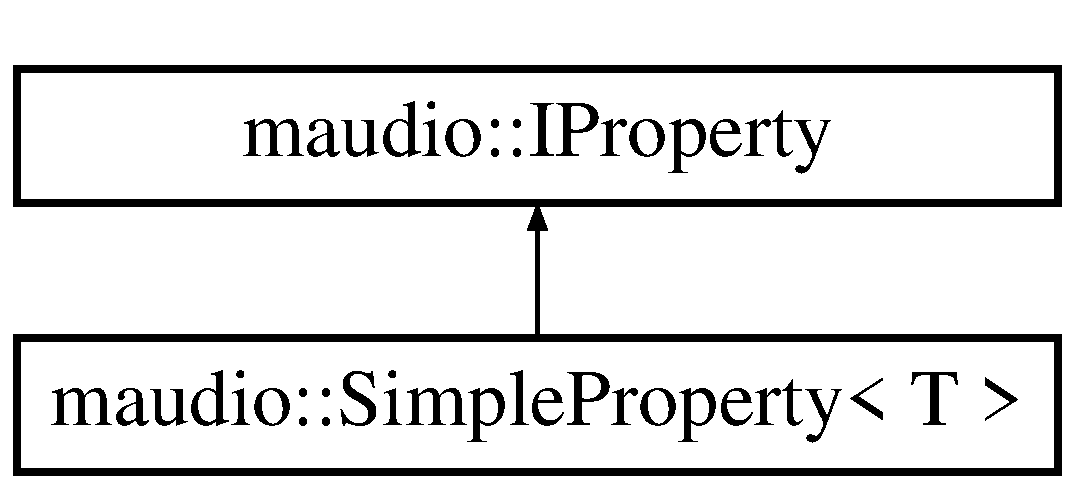
\includegraphics[height=2.000000cm]{classmaudio_1_1SimpleProperty}
\end{center}
\end{figure}
\subsection*{Public Member Functions}
\begin{DoxyCompactItemize}
\item 
\hyperlink{classmaudio_1_1SimpleProperty_a1a611362de067ce51341233d3cd95746}{Simple\-Property} (const char $\ast$name, T value)
\item 
virtual \hyperlink{classmaudio_1_1SimpleProperty_a8c2ec2d4df05f44cbfb480d56cb639f9}{$\sim$\-Simple\-Property} ()
\item 
virtual const char $\ast$ \hyperlink{classmaudio_1_1SimpleProperty_aafd58fa45a18b7b302d526ff267d9db2}{get\-Name} () const 
\item 
virtual const char $\ast$ \hyperlink{classmaudio_1_1SimpleProperty_a12036db02a41a82e49d21a200b04e8b0}{get\-String} () const 
\item 
virtual T \hyperlink{classmaudio_1_1SimpleProperty_aee3d6b2f5a43bd9bdc135d2b9637e937}{get} () const 
\item 
virtual void \hyperlink{classmaudio_1_1SimpleProperty_a8d887f70f8eb17af2e3a667500cf093f}{set} (const std\-::string \&value)
\item 
virtual void \hyperlink{classmaudio_1_1SimpleProperty_a8edb07f2fd51fd60c43a6f35ef45342b}{set} (const char $\ast$value)
\item 
virtual void \hyperlink{classmaudio_1_1SimpleProperty_af1fc590e317ae98e39495977441eb72e}{set} (T value)
\item 
virtual void \hyperlink{classmaudio_1_1SimpleProperty_a830a17d0512fbed31bf015537d1d73f4}{set\-Bounds} (T bottom, T upper)
\item 
virtual const char $\ast$ \hyperlink{classmaudio_1_1SimpleProperty_a6e0133f2b112033ce7519d2f32d913d4}{get\-Bottom\-Bounds\-String} () const 
\item 
virtual const char $\ast$ \hyperlink{classmaudio_1_1SimpleProperty_ac5ccd635686253991acf57d8a2ddbeca}{get\-Upper\-Bounds\-String} () const 
\item 
virtual std\-::vector$<$ std\-::string $>$ \hyperlink{classmaudio_1_1SimpleProperty_a44cac9f0745c6ee80de51f2763d0a96f}{get\-Bounds\-String} () const 
\item 
virtual std\-::vector$<$ T $>$ \hyperlink{classmaudio_1_1SimpleProperty_af034c612b3a3238468e6a17fc7a64632}{get\-Bounds} () const 
\item 
{\footnotesize template$<$$>$ }\\const char $\ast$ \hyperlink{classmaudio_1_1SimpleProperty_a3033164121186a18c5e4bef19bf939de}{get\-String} () const
\item 
{\footnotesize template$<$$>$ }\\void \hyperlink{classmaudio_1_1SimpleProperty_ae8b2e6a1633cf60fb5868e5774b5596a}{set} (std\-::string value)
\item 
{\footnotesize template$<$$>$ }\\void \hyperlink{classmaudio_1_1SimpleProperty_a200fb7cf7cb0380c57b029332f2aff80}{set\-Bounds} (std\-::string bottom, std\-::string upper)
\item 
{\footnotesize template$<$$>$ }\\std\-::vector$<$ std\-::string $>$ \hyperlink{classmaudio_1_1SimpleProperty_a206ab48478c04d3c3711e95c9f5bc00f}{get\-Bounds\-String} () const
\item 
{\footnotesize template$<$$>$ }\\std\-::vector$<$ std\-::string $>$ \hyperlink{classmaudio_1_1SimpleProperty_a2f2e81c25e0f248effb86b1b2f9bc7df}{get\-Bounds} () const
\item 
{\footnotesize template$<$$>$ }\\const char $\ast$ \hyperlink{classmaudio_1_1SimpleProperty_a3033164121186a18c5e4bef19bf939de}{get\-String} () const
\item 
{\footnotesize template$<$$>$ }\\void \hyperlink{classmaudio_1_1SimpleProperty_ae8b2e6a1633cf60fb5868e5774b5596a}{set} (std\-::string value)
\item 
{\footnotesize template$<$$>$ }\\void \hyperlink{classmaudio_1_1SimpleProperty_a200fb7cf7cb0380c57b029332f2aff80}{set\-Bounds} (std\-::string bottom, std\-::string upper)
\item 
{\footnotesize template$<$$>$ }\\std\-::vector$<$ std\-::string $>$ \hyperlink{classmaudio_1_1SimpleProperty_a206ab48478c04d3c3711e95c9f5bc00f}{get\-Bounds\-String} () const
\item 
{\footnotesize template$<$$>$ }\\std\-::vector$<$ std\-::string $>$ \hyperlink{classmaudio_1_1SimpleProperty_a2f2e81c25e0f248effb86b1b2f9bc7df}{get\-Bounds} () const
\end{DoxyCompactItemize}


\subsection{Constructor \& Destructor Documentation}
\hypertarget{classmaudio_1_1SimpleProperty_a1a611362de067ce51341233d3cd95746}{\index{maudio\-::\-Simple\-Property@{maudio\-::\-Simple\-Property}!Simple\-Property@{Simple\-Property}}
\index{Simple\-Property@{Simple\-Property}!maudio::SimpleProperty@{maudio\-::\-Simple\-Property}}
\subsubsection[{Simple\-Property}]{\setlength{\rightskip}{0pt plus 5cm}template$<$typename T $>$ {\bf maudio\-::\-Simple\-Property}$<$ T $>$\-::{\bf Simple\-Property} (
\begin{DoxyParamCaption}
\item[{const char $\ast$}]{name, }
\item[{T}]{value}
\end{DoxyParamCaption}
)}}\label{classmaudio_1_1SimpleProperty_a1a611362de067ce51341233d3cd95746}
\hypertarget{classmaudio_1_1SimpleProperty_a8c2ec2d4df05f44cbfb480d56cb639f9}{\index{maudio\-::\-Simple\-Property@{maudio\-::\-Simple\-Property}!$\sim$\-Simple\-Property@{$\sim$\-Simple\-Property}}
\index{$\sim$\-Simple\-Property@{$\sim$\-Simple\-Property}!maudio::SimpleProperty@{maudio\-::\-Simple\-Property}}
\subsubsection[{$\sim$\-Simple\-Property}]{\setlength{\rightskip}{0pt plus 5cm}template$<$typename T $>$ {\bf maudio\-::\-Simple\-Property}$<$ T $>$\-::$\sim${\bf Simple\-Property} (
\begin{DoxyParamCaption}
{}
\end{DoxyParamCaption}
)\hspace{0.3cm}{\ttfamily [virtual]}}}\label{classmaudio_1_1SimpleProperty_a8c2ec2d4df05f44cbfb480d56cb639f9}


\subsection{Member Function Documentation}
\hypertarget{classmaudio_1_1SimpleProperty_aee3d6b2f5a43bd9bdc135d2b9637e937}{\index{maudio\-::\-Simple\-Property@{maudio\-::\-Simple\-Property}!get@{get}}
\index{get@{get}!maudio::SimpleProperty@{maudio\-::\-Simple\-Property}}
\subsubsection[{get}]{\setlength{\rightskip}{0pt plus 5cm}template$<$typename T $>$ T {\bf maudio\-::\-Simple\-Property}$<$ T $>$\-::get (
\begin{DoxyParamCaption}
{}
\end{DoxyParamCaption}
) const\hspace{0.3cm}{\ttfamily [virtual]}}}\label{classmaudio_1_1SimpleProperty_aee3d6b2f5a43bd9bdc135d2b9637e937}
\hypertarget{classmaudio_1_1SimpleProperty_a6e0133f2b112033ce7519d2f32d913d4}{\index{maudio\-::\-Simple\-Property@{maudio\-::\-Simple\-Property}!get\-Bottom\-Bounds\-String@{get\-Bottom\-Bounds\-String}}
\index{get\-Bottom\-Bounds\-String@{get\-Bottom\-Bounds\-String}!maudio::SimpleProperty@{maudio\-::\-Simple\-Property}}
\subsubsection[{get\-Bottom\-Bounds\-String}]{\setlength{\rightskip}{0pt plus 5cm}template$<$typename T $>$ const char $\ast$ {\bf maudio\-::\-Simple\-Property}$<$ T $>$\-::get\-Bottom\-Bounds\-String (
\begin{DoxyParamCaption}
{}
\end{DoxyParamCaption}
) const\hspace{0.3cm}{\ttfamily [virtual]}}}\label{classmaudio_1_1SimpleProperty_a6e0133f2b112033ce7519d2f32d913d4}


Implements \hyperlink{classmaudio_1_1IProperty_af82e89808ac54aee7a92c182b0ac9e5d}{maudio\-::\-I\-Property}.

\hypertarget{classmaudio_1_1SimpleProperty_af034c612b3a3238468e6a17fc7a64632}{\index{maudio\-::\-Simple\-Property@{maudio\-::\-Simple\-Property}!get\-Bounds@{get\-Bounds}}
\index{get\-Bounds@{get\-Bounds}!maudio::SimpleProperty@{maudio\-::\-Simple\-Property}}
\subsubsection[{get\-Bounds}]{\setlength{\rightskip}{0pt plus 5cm}template$<$typename T $>$ std\-::vector$<$ T $>$ {\bf maudio\-::\-Simple\-Property}$<$ T $>$\-::get\-Bounds (
\begin{DoxyParamCaption}
{}
\end{DoxyParamCaption}
) const\hspace{0.3cm}{\ttfamily [virtual]}}}\label{classmaudio_1_1SimpleProperty_af034c612b3a3238468e6a17fc7a64632}
\hypertarget{classmaudio_1_1SimpleProperty_a2f2e81c25e0f248effb86b1b2f9bc7df}{\index{maudio\-::\-Simple\-Property@{maudio\-::\-Simple\-Property}!get\-Bounds@{get\-Bounds}}
\index{get\-Bounds@{get\-Bounds}!maudio::SimpleProperty@{maudio\-::\-Simple\-Property}}
\subsubsection[{get\-Bounds}]{\setlength{\rightskip}{0pt plus 5cm}template$<$$>$ std\-::vector$<$ std\-::string $>$ {\bf maudio\-::\-Simple\-Property}$<$ std\-::string $>$\-::get\-Bounds (
\begin{DoxyParamCaption}
{}
\end{DoxyParamCaption}
) const}}\label{classmaudio_1_1SimpleProperty_a2f2e81c25e0f248effb86b1b2f9bc7df}
\hypertarget{classmaudio_1_1SimpleProperty_a2f2e81c25e0f248effb86b1b2f9bc7df}{\index{maudio\-::\-Simple\-Property@{maudio\-::\-Simple\-Property}!get\-Bounds@{get\-Bounds}}
\index{get\-Bounds@{get\-Bounds}!maudio::SimpleProperty@{maudio\-::\-Simple\-Property}}
\subsubsection[{get\-Bounds}]{\setlength{\rightskip}{0pt plus 5cm}template$<$$>$ std\-::vector$<$ std\-::string $>$ {\bf maudio\-::\-Simple\-Property}$<$ std\-::string $>$\-::get\-Bounds (
\begin{DoxyParamCaption}
{}
\end{DoxyParamCaption}
) const}}\label{classmaudio_1_1SimpleProperty_a2f2e81c25e0f248effb86b1b2f9bc7df}
\hypertarget{classmaudio_1_1SimpleProperty_a206ab48478c04d3c3711e95c9f5bc00f}{\index{maudio\-::\-Simple\-Property@{maudio\-::\-Simple\-Property}!get\-Bounds\-String@{get\-Bounds\-String}}
\index{get\-Bounds\-String@{get\-Bounds\-String}!maudio::SimpleProperty@{maudio\-::\-Simple\-Property}}
\subsubsection[{get\-Bounds\-String}]{\setlength{\rightskip}{0pt plus 5cm}template$<$$>$ std\-::vector$<$ std\-::string $>$ {\bf maudio\-::\-Simple\-Property}$<$ std\-::string $>$\-::get\-Bounds\-String (
\begin{DoxyParamCaption}
{}
\end{DoxyParamCaption}
) const}}\label{classmaudio_1_1SimpleProperty_a206ab48478c04d3c3711e95c9f5bc00f}
\hypertarget{classmaudio_1_1SimpleProperty_a206ab48478c04d3c3711e95c9f5bc00f}{\index{maudio\-::\-Simple\-Property@{maudio\-::\-Simple\-Property}!get\-Bounds\-String@{get\-Bounds\-String}}
\index{get\-Bounds\-String@{get\-Bounds\-String}!maudio::SimpleProperty@{maudio\-::\-Simple\-Property}}
\subsubsection[{get\-Bounds\-String}]{\setlength{\rightskip}{0pt plus 5cm}template$<$$>$ std\-::vector$<$ std\-::string $>$ {\bf maudio\-::\-Simple\-Property}$<$ std\-::string $>$\-::get\-Bounds\-String (
\begin{DoxyParamCaption}
{}
\end{DoxyParamCaption}
) const}}\label{classmaudio_1_1SimpleProperty_a206ab48478c04d3c3711e95c9f5bc00f}
\hypertarget{classmaudio_1_1SimpleProperty_a44cac9f0745c6ee80de51f2763d0a96f}{\index{maudio\-::\-Simple\-Property@{maudio\-::\-Simple\-Property}!get\-Bounds\-String@{get\-Bounds\-String}}
\index{get\-Bounds\-String@{get\-Bounds\-String}!maudio::SimpleProperty@{maudio\-::\-Simple\-Property}}
\subsubsection[{get\-Bounds\-String}]{\setlength{\rightskip}{0pt plus 5cm}template$<$typename T $>$ std\-::vector$<$ std\-::string $>$ {\bf maudio\-::\-Simple\-Property}$<$ T $>$\-::get\-Bounds\-String (
\begin{DoxyParamCaption}
{}
\end{DoxyParamCaption}
) const\hspace{0.3cm}{\ttfamily [virtual]}}}\label{classmaudio_1_1SimpleProperty_a44cac9f0745c6ee80de51f2763d0a96f}
\hypertarget{classmaudio_1_1SimpleProperty_aafd58fa45a18b7b302d526ff267d9db2}{\index{maudio\-::\-Simple\-Property@{maudio\-::\-Simple\-Property}!get\-Name@{get\-Name}}
\index{get\-Name@{get\-Name}!maudio::SimpleProperty@{maudio\-::\-Simple\-Property}}
\subsubsection[{get\-Name}]{\setlength{\rightskip}{0pt plus 5cm}template$<$typename T $>$ const char $\ast$ {\bf maudio\-::\-Simple\-Property}$<$ T $>$\-::get\-Name (
\begin{DoxyParamCaption}
{}
\end{DoxyParamCaption}
) const\hspace{0.3cm}{\ttfamily [virtual]}}}\label{classmaudio_1_1SimpleProperty_aafd58fa45a18b7b302d526ff267d9db2}


Implements \hyperlink{classmaudio_1_1IProperty_a6f859515ff25325a8a1eb32e76e4e66d}{maudio\-::\-I\-Property}.

\hypertarget{classmaudio_1_1SimpleProperty_a3033164121186a18c5e4bef19bf939de}{\index{maudio\-::\-Simple\-Property@{maudio\-::\-Simple\-Property}!get\-String@{get\-String}}
\index{get\-String@{get\-String}!maudio::SimpleProperty@{maudio\-::\-Simple\-Property}}
\subsubsection[{get\-String}]{\setlength{\rightskip}{0pt plus 5cm}template$<$$>$ const char $\ast$ {\bf maudio\-::\-Simple\-Property}$<$ bool $>$\-::get\-String (
\begin{DoxyParamCaption}
{}
\end{DoxyParamCaption}
) const\hspace{0.3cm}{\ttfamily [virtual]}}}\label{classmaudio_1_1SimpleProperty_a3033164121186a18c5e4bef19bf939de}


Implements \hyperlink{classmaudio_1_1IProperty_a7964046c2be4eceb88021f0ab059f159}{maudio\-::\-I\-Property}.

\hypertarget{classmaudio_1_1SimpleProperty_a3033164121186a18c5e4bef19bf939de}{\index{maudio\-::\-Simple\-Property@{maudio\-::\-Simple\-Property}!get\-String@{get\-String}}
\index{get\-String@{get\-String}!maudio::SimpleProperty@{maudio\-::\-Simple\-Property}}
\subsubsection[{get\-String}]{\setlength{\rightskip}{0pt plus 5cm}template$<$$>$ const char $\ast$ {\bf maudio\-::\-Simple\-Property}$<$ bool $>$\-::get\-String (
\begin{DoxyParamCaption}
{}
\end{DoxyParamCaption}
) const\hspace{0.3cm}{\ttfamily [virtual]}}}\label{classmaudio_1_1SimpleProperty_a3033164121186a18c5e4bef19bf939de}


Implements \hyperlink{classmaudio_1_1IProperty_a7964046c2be4eceb88021f0ab059f159}{maudio\-::\-I\-Property}.

\hypertarget{classmaudio_1_1SimpleProperty_a12036db02a41a82e49d21a200b04e8b0}{\index{maudio\-::\-Simple\-Property@{maudio\-::\-Simple\-Property}!get\-String@{get\-String}}
\index{get\-String@{get\-String}!maudio::SimpleProperty@{maudio\-::\-Simple\-Property}}
\subsubsection[{get\-String}]{\setlength{\rightskip}{0pt plus 5cm}template$<$typename T $>$ const char $\ast$ {\bf maudio\-::\-Simple\-Property}$<$ T $>$\-::get\-String (
\begin{DoxyParamCaption}
{}
\end{DoxyParamCaption}
) const\hspace{0.3cm}{\ttfamily [virtual]}}}\label{classmaudio_1_1SimpleProperty_a12036db02a41a82e49d21a200b04e8b0}


Implements \hyperlink{classmaudio_1_1IProperty_a7964046c2be4eceb88021f0ab059f159}{maudio\-::\-I\-Property}.

\hypertarget{classmaudio_1_1SimpleProperty_ac5ccd635686253991acf57d8a2ddbeca}{\index{maudio\-::\-Simple\-Property@{maudio\-::\-Simple\-Property}!get\-Upper\-Bounds\-String@{get\-Upper\-Bounds\-String}}
\index{get\-Upper\-Bounds\-String@{get\-Upper\-Bounds\-String}!maudio::SimpleProperty@{maudio\-::\-Simple\-Property}}
\subsubsection[{get\-Upper\-Bounds\-String}]{\setlength{\rightskip}{0pt plus 5cm}template$<$typename T $>$ const char $\ast$ {\bf maudio\-::\-Simple\-Property}$<$ T $>$\-::get\-Upper\-Bounds\-String (
\begin{DoxyParamCaption}
{}
\end{DoxyParamCaption}
) const\hspace{0.3cm}{\ttfamily [virtual]}}}\label{classmaudio_1_1SimpleProperty_ac5ccd635686253991acf57d8a2ddbeca}


Implements \hyperlink{classmaudio_1_1IProperty_a4182ebf0441cf1d3927e222331f00e93}{maudio\-::\-I\-Property}.

\hypertarget{classmaudio_1_1SimpleProperty_ae8b2e6a1633cf60fb5868e5774b5596a}{\index{maudio\-::\-Simple\-Property@{maudio\-::\-Simple\-Property}!set@{set}}
\index{set@{set}!maudio::SimpleProperty@{maudio\-::\-Simple\-Property}}
\subsubsection[{set}]{\setlength{\rightskip}{0pt plus 5cm}template$<$$>$ void {\bf maudio\-::\-Simple\-Property}$<$ std\-::string $>$\-::set (
\begin{DoxyParamCaption}
\item[{std\-::string}]{value}
\end{DoxyParamCaption}
)}}\label{classmaudio_1_1SimpleProperty_ae8b2e6a1633cf60fb5868e5774b5596a}
\hypertarget{classmaudio_1_1SimpleProperty_ae8b2e6a1633cf60fb5868e5774b5596a}{\index{maudio\-::\-Simple\-Property@{maudio\-::\-Simple\-Property}!set@{set}}
\index{set@{set}!maudio::SimpleProperty@{maudio\-::\-Simple\-Property}}
\subsubsection[{set}]{\setlength{\rightskip}{0pt plus 5cm}template$<$$>$ void {\bf maudio\-::\-Simple\-Property}$<$ std\-::string $>$\-::set (
\begin{DoxyParamCaption}
\item[{std\-::string}]{value}
\end{DoxyParamCaption}
)}}\label{classmaudio_1_1SimpleProperty_ae8b2e6a1633cf60fb5868e5774b5596a}
\hypertarget{classmaudio_1_1SimpleProperty_a8d887f70f8eb17af2e3a667500cf093f}{\index{maudio\-::\-Simple\-Property@{maudio\-::\-Simple\-Property}!set@{set}}
\index{set@{set}!maudio::SimpleProperty@{maudio\-::\-Simple\-Property}}
\subsubsection[{set}]{\setlength{\rightskip}{0pt plus 5cm}template$<$typename T $>$ void {\bf maudio\-::\-Simple\-Property}$<$ T $>$\-::set (
\begin{DoxyParamCaption}
\item[{const std\-::string \&}]{value}
\end{DoxyParamCaption}
)\hspace{0.3cm}{\ttfamily [virtual]}}}\label{classmaudio_1_1SimpleProperty_a8d887f70f8eb17af2e3a667500cf093f}
\hypertarget{classmaudio_1_1SimpleProperty_a8edb07f2fd51fd60c43a6f35ef45342b}{\index{maudio\-::\-Simple\-Property@{maudio\-::\-Simple\-Property}!set@{set}}
\index{set@{set}!maudio::SimpleProperty@{maudio\-::\-Simple\-Property}}
\subsubsection[{set}]{\setlength{\rightskip}{0pt plus 5cm}template$<$typename T $>$ void {\bf maudio\-::\-Simple\-Property}$<$ T $>$\-::set (
\begin{DoxyParamCaption}
\item[{const char $\ast$}]{value}
\end{DoxyParamCaption}
)\hspace{0.3cm}{\ttfamily [virtual]}}}\label{classmaudio_1_1SimpleProperty_a8edb07f2fd51fd60c43a6f35ef45342b}


Implements \hyperlink{classmaudio_1_1IProperty_aeb474ef1dd68fd14d88de535eff92d0f}{maudio\-::\-I\-Property}.

\hypertarget{classmaudio_1_1SimpleProperty_af1fc590e317ae98e39495977441eb72e}{\index{maudio\-::\-Simple\-Property@{maudio\-::\-Simple\-Property}!set@{set}}
\index{set@{set}!maudio::SimpleProperty@{maudio\-::\-Simple\-Property}}
\subsubsection[{set}]{\setlength{\rightskip}{0pt plus 5cm}template$<$typename T $>$ void {\bf maudio\-::\-Simple\-Property}$<$ T $>$\-::set (
\begin{DoxyParamCaption}
\item[{T}]{value}
\end{DoxyParamCaption}
)\hspace{0.3cm}{\ttfamily [virtual]}}}\label{classmaudio_1_1SimpleProperty_af1fc590e317ae98e39495977441eb72e}
\hypertarget{classmaudio_1_1SimpleProperty_a200fb7cf7cb0380c57b029332f2aff80}{\index{maudio\-::\-Simple\-Property@{maudio\-::\-Simple\-Property}!set\-Bounds@{set\-Bounds}}
\index{set\-Bounds@{set\-Bounds}!maudio::SimpleProperty@{maudio\-::\-Simple\-Property}}
\subsubsection[{set\-Bounds}]{\setlength{\rightskip}{0pt plus 5cm}template$<$$>$ void {\bf maudio\-::\-Simple\-Property}$<$ std\-::string $>$\-::set\-Bounds (
\begin{DoxyParamCaption}
\item[{std\-::string}]{bottom, }
\item[{std\-::string}]{upper}
\end{DoxyParamCaption}
)}}\label{classmaudio_1_1SimpleProperty_a200fb7cf7cb0380c57b029332f2aff80}
\hypertarget{classmaudio_1_1SimpleProperty_a200fb7cf7cb0380c57b029332f2aff80}{\index{maudio\-::\-Simple\-Property@{maudio\-::\-Simple\-Property}!set\-Bounds@{set\-Bounds}}
\index{set\-Bounds@{set\-Bounds}!maudio::SimpleProperty@{maudio\-::\-Simple\-Property}}
\subsubsection[{set\-Bounds}]{\setlength{\rightskip}{0pt plus 5cm}template$<$$>$ void {\bf maudio\-::\-Simple\-Property}$<$ std\-::string $>$\-::set\-Bounds (
\begin{DoxyParamCaption}
\item[{std\-::string}]{bottom, }
\item[{std\-::string}]{upper}
\end{DoxyParamCaption}
)}}\label{classmaudio_1_1SimpleProperty_a200fb7cf7cb0380c57b029332f2aff80}
\hypertarget{classmaudio_1_1SimpleProperty_a830a17d0512fbed31bf015537d1d73f4}{\index{maudio\-::\-Simple\-Property@{maudio\-::\-Simple\-Property}!set\-Bounds@{set\-Bounds}}
\index{set\-Bounds@{set\-Bounds}!maudio::SimpleProperty@{maudio\-::\-Simple\-Property}}
\subsubsection[{set\-Bounds}]{\setlength{\rightskip}{0pt plus 5cm}template$<$typename T $>$ void {\bf maudio\-::\-Simple\-Property}$<$ T $>$\-::set\-Bounds (
\begin{DoxyParamCaption}
\item[{T}]{bottom, }
\item[{T}]{upper}
\end{DoxyParamCaption}
)\hspace{0.3cm}{\ttfamily [virtual]}}}\label{classmaudio_1_1SimpleProperty_a830a17d0512fbed31bf015537d1d73f4}


The documentation for this class was generated from the following file\-:\begin{DoxyCompactItemize}
\item 
/home/mars/\-Projekte/maudio/src/plugins/include/core/property/\hyperlink{SimpleProperty_8hpp}{Simple\-Property.\-hpp}\end{DoxyCompactItemize}

\hypertarget{classmaudio_1_1SinusGenerator}{\section{maudio\-:\-:Sinus\-Generator Class Reference}
\label{classmaudio_1_1SinusGenerator}\index{maudio\-::\-Sinus\-Generator@{maudio\-::\-Sinus\-Generator}}
}


{\ttfamily \#include $<$Sinus\-Generator.\-hpp$>$}

Inheritance diagram for maudio\-:\-:Sinus\-Generator\-:\begin{figure}[H]
\begin{center}
\leavevmode
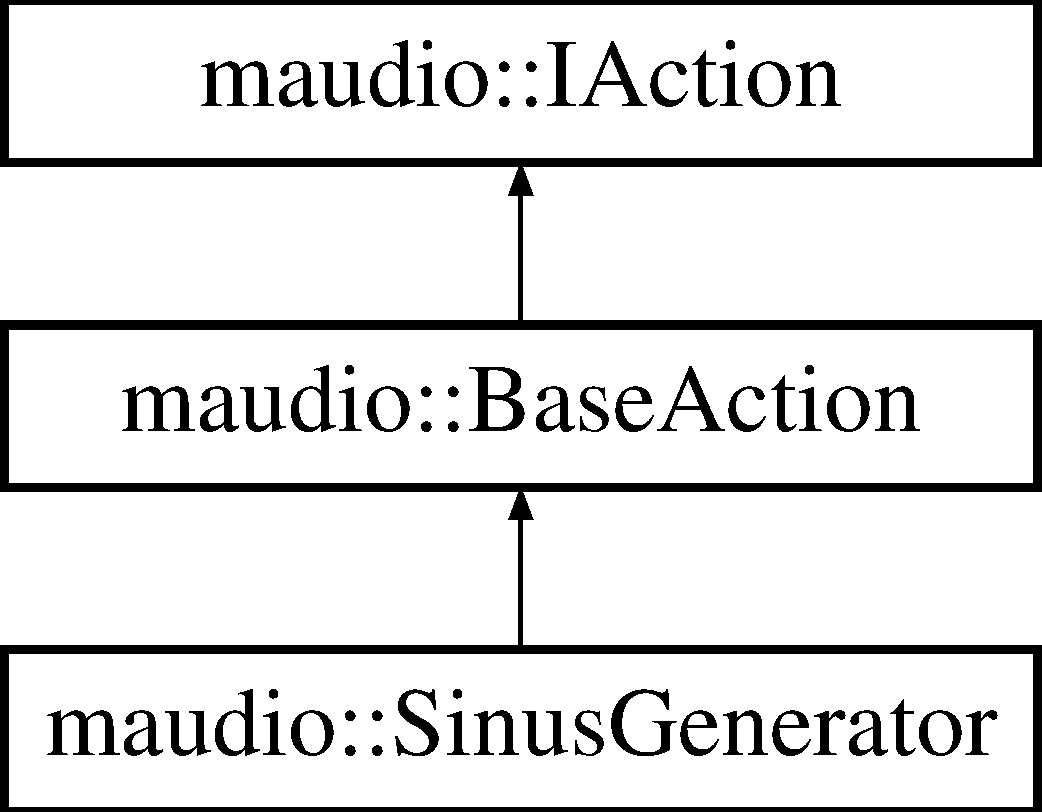
\includegraphics[height=3.000000cm]{classmaudio_1_1SinusGenerator}
\end{center}
\end{figure}
\subsection*{Public Member Functions}
\begin{DoxyCompactItemize}
\item 
\hyperlink{classmaudio_1_1SinusGenerator_a2a6f8d9cbb43ae177e50ba5e64e53a3c}{Sinus\-Generator} ()
\item 
virtual \hyperlink{classmaudio_1_1SinusGenerator_aed11cbd52f1ee60ef9819478182b58e4}{$\sim$\-Sinus\-Generator} ()
\item 
virtual \hyperlink{classmaudio_1_1IAudioBuffer}{I\-Audio\-Buffer} $\ast$ \hyperlink{classmaudio_1_1SinusGenerator_a461fdc87ced846928ea651173122713a}{get} (unsigned long pos, unsigned int length) noexcept
\item 
virtual \hyperlink{classmaudio_1_1IAudioInfo}{I\-Audio\-Info} $\ast$ \hyperlink{classmaudio_1_1SinusGenerator_ab3ac1d0f6d84658262026bbebcbd808f}{get\-Info} () noexcept
\item 
virtual int \hyperlink{classmaudio_1_1SinusGenerator_aee038f2dd2415a96ce1902be978f4ad4}{Max\-Inputs} () const 
\item 
virtual bool \hyperlink{classmaudio_1_1SinusGenerator_a0e39f15f11221f97fb034a42df608889}{Has\-Outputs} () const 
\item 
virtual void \hyperlink{classmaudio_1_1SinusGenerator_a9a901592dba8df35ac74ddd85cbb1482}{read\-Config} (const \hyperlink{classmaudio_1_1IKeyValueStore}{I\-Key\-Value\-Store} \&conf)
\item 
virtual void \hyperlink{classmaudio_1_1SinusGenerator_a7957a8e22bbda999d99cb5dc954a6979}{set\-Frequency} (float freq)
\item 
virtual void \hyperlink{classmaudio_1_1SinusGenerator_a5b75c779c1a8f249e70a442d591e7b41}{set\-Samplerate} (unsigned int samplerate)
\item 
virtual void \hyperlink{classmaudio_1_1SinusGenerator_a13aa66a1d01fec78d92c9b05c1d111d7}{set\-Channels} (unsigned int channels)
\end{DoxyCompactItemize}
\subsection*{Additional Inherited Members}


\subsection{Constructor \& Destructor Documentation}
\hypertarget{classmaudio_1_1SinusGenerator_a2a6f8d9cbb43ae177e50ba5e64e53a3c}{\index{maudio\-::\-Sinus\-Generator@{maudio\-::\-Sinus\-Generator}!Sinus\-Generator@{Sinus\-Generator}}
\index{Sinus\-Generator@{Sinus\-Generator}!maudio::SinusGenerator@{maudio\-::\-Sinus\-Generator}}
\subsubsection[{Sinus\-Generator}]{\setlength{\rightskip}{0pt plus 5cm}maudio\-::\-Sinus\-Generator\-::\-Sinus\-Generator (
\begin{DoxyParamCaption}
{}
\end{DoxyParamCaption}
)}}\label{classmaudio_1_1SinusGenerator_a2a6f8d9cbb43ae177e50ba5e64e53a3c}
\hypertarget{classmaudio_1_1SinusGenerator_aed11cbd52f1ee60ef9819478182b58e4}{\index{maudio\-::\-Sinus\-Generator@{maudio\-::\-Sinus\-Generator}!$\sim$\-Sinus\-Generator@{$\sim$\-Sinus\-Generator}}
\index{$\sim$\-Sinus\-Generator@{$\sim$\-Sinus\-Generator}!maudio::SinusGenerator@{maudio\-::\-Sinus\-Generator}}
\subsubsection[{$\sim$\-Sinus\-Generator}]{\setlength{\rightskip}{0pt plus 5cm}maudio\-::\-Sinus\-Generator\-::$\sim$\-Sinus\-Generator (
\begin{DoxyParamCaption}
{}
\end{DoxyParamCaption}
)\hspace{0.3cm}{\ttfamily [virtual]}}}\label{classmaudio_1_1SinusGenerator_aed11cbd52f1ee60ef9819478182b58e4}


\subsection{Member Function Documentation}
\hypertarget{classmaudio_1_1SinusGenerator_a461fdc87ced846928ea651173122713a}{\index{maudio\-::\-Sinus\-Generator@{maudio\-::\-Sinus\-Generator}!get@{get}}
\index{get@{get}!maudio::SinusGenerator@{maudio\-::\-Sinus\-Generator}}
\subsubsection[{get}]{\setlength{\rightskip}{0pt plus 5cm}{\bf I\-Audio\-Buffer} $\ast$ maudio\-::\-Sinus\-Generator\-::get (
\begin{DoxyParamCaption}
\item[{unsigned long}]{pos, }
\item[{unsigned int}]{length}
\end{DoxyParamCaption}
)\hspace{0.3cm}{\ttfamily [virtual]}, {\ttfamily [noexcept]}}}\label{classmaudio_1_1SinusGenerator_a461fdc87ced846928ea651173122713a}


Implements \hyperlink{classmaudio_1_1IAction_adcd159456456b1104af6d4f31336fe59}{maudio\-::\-I\-Action}.

\hypertarget{classmaudio_1_1SinusGenerator_ab3ac1d0f6d84658262026bbebcbd808f}{\index{maudio\-::\-Sinus\-Generator@{maudio\-::\-Sinus\-Generator}!get\-Info@{get\-Info}}
\index{get\-Info@{get\-Info}!maudio::SinusGenerator@{maudio\-::\-Sinus\-Generator}}
\subsubsection[{get\-Info}]{\setlength{\rightskip}{0pt plus 5cm}{\bf I\-Audio\-Info} $\ast$ maudio\-::\-Sinus\-Generator\-::get\-Info (
\begin{DoxyParamCaption}
{}
\end{DoxyParamCaption}
)\hspace{0.3cm}{\ttfamily [virtual]}, {\ttfamily [noexcept]}}}\label{classmaudio_1_1SinusGenerator_ab3ac1d0f6d84658262026bbebcbd808f}


Implements \hyperlink{classmaudio_1_1IAction_abf9d7d1a4d66fd1b48d946d672bfe7a0}{maudio\-::\-I\-Action}.

\hypertarget{classmaudio_1_1SinusGenerator_a0e39f15f11221f97fb034a42df608889}{\index{maudio\-::\-Sinus\-Generator@{maudio\-::\-Sinus\-Generator}!Has\-Outputs@{Has\-Outputs}}
\index{Has\-Outputs@{Has\-Outputs}!maudio::SinusGenerator@{maudio\-::\-Sinus\-Generator}}
\subsubsection[{Has\-Outputs}]{\setlength{\rightskip}{0pt plus 5cm}bool maudio\-::\-Sinus\-Generator\-::\-Has\-Outputs (
\begin{DoxyParamCaption}
{}
\end{DoxyParamCaption}
) const\hspace{0.3cm}{\ttfamily [virtual]}}}\label{classmaudio_1_1SinusGenerator_a0e39f15f11221f97fb034a42df608889}


Implements \hyperlink{classmaudio_1_1IAction_a148ec76547dc1ac21e47b4b5d10c152a}{maudio\-::\-I\-Action}.

\hypertarget{classmaudio_1_1SinusGenerator_aee038f2dd2415a96ce1902be978f4ad4}{\index{maudio\-::\-Sinus\-Generator@{maudio\-::\-Sinus\-Generator}!Max\-Inputs@{Max\-Inputs}}
\index{Max\-Inputs@{Max\-Inputs}!maudio::SinusGenerator@{maudio\-::\-Sinus\-Generator}}
\subsubsection[{Max\-Inputs}]{\setlength{\rightskip}{0pt plus 5cm}int maudio\-::\-Sinus\-Generator\-::\-Max\-Inputs (
\begin{DoxyParamCaption}
{}
\end{DoxyParamCaption}
) const\hspace{0.3cm}{\ttfamily [virtual]}}}\label{classmaudio_1_1SinusGenerator_aee038f2dd2415a96ce1902be978f4ad4}


Implements \hyperlink{classmaudio_1_1IAction_a3c8825e7f38e0de769af7d81ccf6cf5e}{maudio\-::\-I\-Action}.

\hypertarget{classmaudio_1_1SinusGenerator_a9a901592dba8df35ac74ddd85cbb1482}{\index{maudio\-::\-Sinus\-Generator@{maudio\-::\-Sinus\-Generator}!read\-Config@{read\-Config}}
\index{read\-Config@{read\-Config}!maudio::SinusGenerator@{maudio\-::\-Sinus\-Generator}}
\subsubsection[{read\-Config}]{\setlength{\rightskip}{0pt plus 5cm}void maudio\-::\-Sinus\-Generator\-::read\-Config (
\begin{DoxyParamCaption}
\item[{const {\bf I\-Key\-Value\-Store} \&}]{conf}
\end{DoxyParamCaption}
)\hspace{0.3cm}{\ttfamily [virtual]}}}\label{classmaudio_1_1SinusGenerator_a9a901592dba8df35ac74ddd85cbb1482}


Implements \hyperlink{classmaudio_1_1IAction_a610804d37c46509f3eaa1aebceab7e35}{maudio\-::\-I\-Action}.

\hypertarget{classmaudio_1_1SinusGenerator_a13aa66a1d01fec78d92c9b05c1d111d7}{\index{maudio\-::\-Sinus\-Generator@{maudio\-::\-Sinus\-Generator}!set\-Channels@{set\-Channels}}
\index{set\-Channels@{set\-Channels}!maudio::SinusGenerator@{maudio\-::\-Sinus\-Generator}}
\subsubsection[{set\-Channels}]{\setlength{\rightskip}{0pt plus 5cm}void maudio\-::\-Sinus\-Generator\-::set\-Channels (
\begin{DoxyParamCaption}
\item[{unsigned int}]{channels}
\end{DoxyParamCaption}
)\hspace{0.3cm}{\ttfamily [virtual]}}}\label{classmaudio_1_1SinusGenerator_a13aa66a1d01fec78d92c9b05c1d111d7}
\hypertarget{classmaudio_1_1SinusGenerator_a7957a8e22bbda999d99cb5dc954a6979}{\index{maudio\-::\-Sinus\-Generator@{maudio\-::\-Sinus\-Generator}!set\-Frequency@{set\-Frequency}}
\index{set\-Frequency@{set\-Frequency}!maudio::SinusGenerator@{maudio\-::\-Sinus\-Generator}}
\subsubsection[{set\-Frequency}]{\setlength{\rightskip}{0pt plus 5cm}void maudio\-::\-Sinus\-Generator\-::set\-Frequency (
\begin{DoxyParamCaption}
\item[{float}]{freq}
\end{DoxyParamCaption}
)\hspace{0.3cm}{\ttfamily [virtual]}}}\label{classmaudio_1_1SinusGenerator_a7957a8e22bbda999d99cb5dc954a6979}
\hypertarget{classmaudio_1_1SinusGenerator_a5b75c779c1a8f249e70a442d591e7b41}{\index{maudio\-::\-Sinus\-Generator@{maudio\-::\-Sinus\-Generator}!set\-Samplerate@{set\-Samplerate}}
\index{set\-Samplerate@{set\-Samplerate}!maudio::SinusGenerator@{maudio\-::\-Sinus\-Generator}}
\subsubsection[{set\-Samplerate}]{\setlength{\rightskip}{0pt plus 5cm}void maudio\-::\-Sinus\-Generator\-::set\-Samplerate (
\begin{DoxyParamCaption}
\item[{unsigned int}]{samplerate}
\end{DoxyParamCaption}
)\hspace{0.3cm}{\ttfamily [virtual]}}}\label{classmaudio_1_1SinusGenerator_a5b75c779c1a8f249e70a442d591e7b41}


The documentation for this class was generated from the following files\-:\begin{DoxyCompactItemize}
\item 
/home/mars/\-Projekte/maudio/src/plugins/include/core/actions/\hyperlink{SinusGenerator_8hpp}{Sinus\-Generator.\-hpp}\item 
/home/mars/\-Projekte/maudio/src/core/actions/\hyperlink{core_2actions_2SinusGenerator_8cpp}{Sinus\-Generator.\-cpp}\end{DoxyCompactItemize}

\hypertarget{classmaudio_1_1ActionNode_1_1Socket}{\section{maudio\-:\-:Action\-Node\-:\-:Socket Class Reference}
\label{classmaudio_1_1ActionNode_1_1Socket}\index{maudio\-::\-Action\-Node\-::\-Socket@{maudio\-::\-Action\-Node\-::\-Socket}}
}


{\ttfamily \#include $<$Action\-Node.\-hpp$>$}

Inheritance diagram for maudio\-:\-:Action\-Node\-:\-:Socket\-:\begin{figure}[H]
\begin{center}
\leavevmode
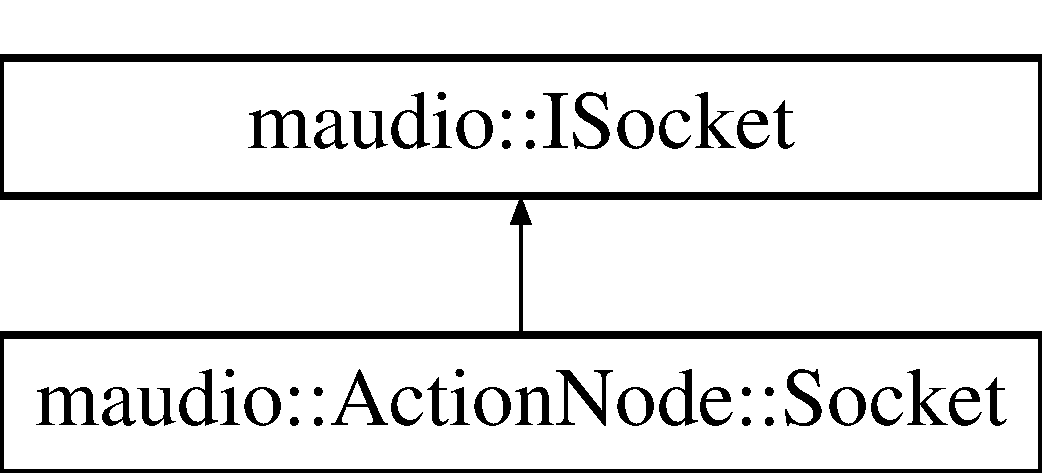
\includegraphics[height=2.000000cm]{classmaudio_1_1ActionNode_1_1Socket}
\end{center}
\end{figure}
\subsection*{Public Member Functions}
\begin{DoxyCompactItemize}
\item 
\hyperlink{classmaudio_1_1ActionNode_1_1Socket_a3c1f70a4d60050e19cf3ecb441068653}{Socket} (std\-::shared\-\_\-ptr$<$ \hyperlink{classmaudio_1_1Node}{Node} $>$ input)
\item 
virtual \hyperlink{classmaudio_1_1ActionNode_1_1Socket_a184298687b5653972217b83afe6425d9}{$\sim$\-Socket} ()
\item 
virtual \hyperlink{classmaudio_1_1IAudioBuffer}{I\-Audio\-Buffer} $\ast$ \hyperlink{classmaudio_1_1ActionNode_1_1Socket_a3801dbf1ff87f6f4d417d2929ff3c107}{get} (unsigned long pos, unsigned int length) noexcept
\item 
virtual \hyperlink{classmaudio_1_1IAudioInfo}{I\-Audio\-Info} $\ast$ \hyperlink{classmaudio_1_1ActionNode_1_1Socket_adf54bb1504b5cf9d53fe6529e86e3653}{get\-Info} () noexcept
\item 
virtual void \hyperlink{classmaudio_1_1ActionNode_1_1Socket_a8a64ba64966caca18a70c711ff1e4b2d}{delete\-Buffer} (\hyperlink{classmaudio_1_1IAudioBuffer}{I\-Audio\-Buffer} $\ast$data) noexcept
\item 
virtual void \hyperlink{classmaudio_1_1ActionNode_1_1Socket_a3e25c1d6d28ecbfdfeecd6b6c846a1be}{delete\-Info} (\hyperlink{classmaudio_1_1IAudioInfo}{I\-Audio\-Info} $\ast$data) noexcept
\item 
virtual void \hyperlink{classmaudio_1_1ActionNode_1_1Socket_a8882eaaf8ea9d06ea006c6d977acdeb7}{delete\-Sample} (\hyperlink{classmaudio_1_1ISample}{I\-Sample} $\ast$data) noexcept
\end{DoxyCompactItemize}


\subsection{Constructor \& Destructor Documentation}
\hypertarget{classmaudio_1_1ActionNode_1_1Socket_a3c1f70a4d60050e19cf3ecb441068653}{\index{maudio\-::\-Action\-Node\-::\-Socket@{maudio\-::\-Action\-Node\-::\-Socket}!Socket@{Socket}}
\index{Socket@{Socket}!maudio::ActionNode::Socket@{maudio\-::\-Action\-Node\-::\-Socket}}
\subsubsection[{Socket}]{\setlength{\rightskip}{0pt plus 5cm}maudio\-::\-Action\-Node\-::\-Socket\-::\-Socket (
\begin{DoxyParamCaption}
\item[{std\-::shared\-\_\-ptr$<$ {\bf Node} $>$}]{input}
\end{DoxyParamCaption}
)}}\label{classmaudio_1_1ActionNode_1_1Socket_a3c1f70a4d60050e19cf3ecb441068653}
\hypertarget{classmaudio_1_1ActionNode_1_1Socket_a184298687b5653972217b83afe6425d9}{\index{maudio\-::\-Action\-Node\-::\-Socket@{maudio\-::\-Action\-Node\-::\-Socket}!$\sim$\-Socket@{$\sim$\-Socket}}
\index{$\sim$\-Socket@{$\sim$\-Socket}!maudio::ActionNode::Socket@{maudio\-::\-Action\-Node\-::\-Socket}}
\subsubsection[{$\sim$\-Socket}]{\setlength{\rightskip}{0pt plus 5cm}maudio\-::\-Action\-Node\-::\-Socket\-::$\sim$\-Socket (
\begin{DoxyParamCaption}
{}
\end{DoxyParamCaption}
)\hspace{0.3cm}{\ttfamily [virtual]}}}\label{classmaudio_1_1ActionNode_1_1Socket_a184298687b5653972217b83afe6425d9}


\subsection{Member Function Documentation}
\hypertarget{classmaudio_1_1ActionNode_1_1Socket_a8a64ba64966caca18a70c711ff1e4b2d}{\index{maudio\-::\-Action\-Node\-::\-Socket@{maudio\-::\-Action\-Node\-::\-Socket}!delete\-Buffer@{delete\-Buffer}}
\index{delete\-Buffer@{delete\-Buffer}!maudio::ActionNode::Socket@{maudio\-::\-Action\-Node\-::\-Socket}}
\subsubsection[{delete\-Buffer}]{\setlength{\rightskip}{0pt plus 5cm}void maudio\-::\-Action\-Node\-::\-Socket\-::delete\-Buffer (
\begin{DoxyParamCaption}
\item[{{\bf I\-Audio\-Buffer} $\ast$}]{data}
\end{DoxyParamCaption}
)\hspace{0.3cm}{\ttfamily [virtual]}, {\ttfamily [noexcept]}}}\label{classmaudio_1_1ActionNode_1_1Socket_a8a64ba64966caca18a70c711ff1e4b2d}


Implements \hyperlink{classmaudio_1_1ISocket_a8015c32967e28f35c6abdbe979e4f318}{maudio\-::\-I\-Socket}.

\hypertarget{classmaudio_1_1ActionNode_1_1Socket_a3e25c1d6d28ecbfdfeecd6b6c846a1be}{\index{maudio\-::\-Action\-Node\-::\-Socket@{maudio\-::\-Action\-Node\-::\-Socket}!delete\-Info@{delete\-Info}}
\index{delete\-Info@{delete\-Info}!maudio::ActionNode::Socket@{maudio\-::\-Action\-Node\-::\-Socket}}
\subsubsection[{delete\-Info}]{\setlength{\rightskip}{0pt plus 5cm}void maudio\-::\-Action\-Node\-::\-Socket\-::delete\-Info (
\begin{DoxyParamCaption}
\item[{{\bf I\-Audio\-Info} $\ast$}]{data}
\end{DoxyParamCaption}
)\hspace{0.3cm}{\ttfamily [virtual]}, {\ttfamily [noexcept]}}}\label{classmaudio_1_1ActionNode_1_1Socket_a3e25c1d6d28ecbfdfeecd6b6c846a1be}


Implements \hyperlink{classmaudio_1_1ISocket_a180a1cb55da56375612a5bdc53be61ee}{maudio\-::\-I\-Socket}.

\hypertarget{classmaudio_1_1ActionNode_1_1Socket_a8882eaaf8ea9d06ea006c6d977acdeb7}{\index{maudio\-::\-Action\-Node\-::\-Socket@{maudio\-::\-Action\-Node\-::\-Socket}!delete\-Sample@{delete\-Sample}}
\index{delete\-Sample@{delete\-Sample}!maudio::ActionNode::Socket@{maudio\-::\-Action\-Node\-::\-Socket}}
\subsubsection[{delete\-Sample}]{\setlength{\rightskip}{0pt plus 5cm}void maudio\-::\-Action\-Node\-::\-Socket\-::delete\-Sample (
\begin{DoxyParamCaption}
\item[{{\bf I\-Sample} $\ast$}]{data}
\end{DoxyParamCaption}
)\hspace{0.3cm}{\ttfamily [virtual]}, {\ttfamily [noexcept]}}}\label{classmaudio_1_1ActionNode_1_1Socket_a8882eaaf8ea9d06ea006c6d977acdeb7}


Implements \hyperlink{classmaudio_1_1ISocket_ae67025d3d0befc48cbfd11bd05da1386}{maudio\-::\-I\-Socket}.

\hypertarget{classmaudio_1_1ActionNode_1_1Socket_a3801dbf1ff87f6f4d417d2929ff3c107}{\index{maudio\-::\-Action\-Node\-::\-Socket@{maudio\-::\-Action\-Node\-::\-Socket}!get@{get}}
\index{get@{get}!maudio::ActionNode::Socket@{maudio\-::\-Action\-Node\-::\-Socket}}
\subsubsection[{get}]{\setlength{\rightskip}{0pt plus 5cm}{\bf I\-Audio\-Buffer} $\ast$ maudio\-::\-Action\-Node\-::\-Socket\-::get (
\begin{DoxyParamCaption}
\item[{unsigned long}]{pos, }
\item[{unsigned int}]{length}
\end{DoxyParamCaption}
)\hspace{0.3cm}{\ttfamily [virtual]}, {\ttfamily [noexcept]}}}\label{classmaudio_1_1ActionNode_1_1Socket_a3801dbf1ff87f6f4d417d2929ff3c107}


Implements \hyperlink{classmaudio_1_1ISocket_a6a2d1f172963b079563c015ae7338db1}{maudio\-::\-I\-Socket}.

\hypertarget{classmaudio_1_1ActionNode_1_1Socket_adf54bb1504b5cf9d53fe6529e86e3653}{\index{maudio\-::\-Action\-Node\-::\-Socket@{maudio\-::\-Action\-Node\-::\-Socket}!get\-Info@{get\-Info}}
\index{get\-Info@{get\-Info}!maudio::ActionNode::Socket@{maudio\-::\-Action\-Node\-::\-Socket}}
\subsubsection[{get\-Info}]{\setlength{\rightskip}{0pt plus 5cm}{\bf I\-Audio\-Info} $\ast$ maudio\-::\-Action\-Node\-::\-Socket\-::get\-Info (
\begin{DoxyParamCaption}
{}
\end{DoxyParamCaption}
)\hspace{0.3cm}{\ttfamily [virtual]}, {\ttfamily [noexcept]}}}\label{classmaudio_1_1ActionNode_1_1Socket_adf54bb1504b5cf9d53fe6529e86e3653}


Implements \hyperlink{classmaudio_1_1ISocket_a43b1b9ab16b93131ba7d11204cbe5558}{maudio\-::\-I\-Socket}.



The documentation for this class was generated from the following files\-:\begin{DoxyCompactItemize}
\item 
/home/mars/\-Projekte/maudio/src/plugins/include/core/node/\hyperlink{ActionNode_8hpp}{Action\-Node.\-hpp}\item 
/home/mars/\-Projekte/maudio/src/core/node/\hyperlink{core_2node_2ActionNode_8cpp}{Action\-Node.\-cpp}\end{DoxyCompactItemize}

\hypertarget{classmaudio_1_1String}{\section{maudio\-:\-:String Class Reference}
\label{classmaudio_1_1String}\index{maudio\-::\-String@{maudio\-::\-String}}
}


\hyperlink{classmaudio_1_1String}{String} class that takes ownership of char $\ast$ on assignment.  




{\ttfamily \#include $<$String.\-hpp$>$}

\subsection*{Public Member Functions}
\begin{DoxyCompactItemize}
\item 
\hyperlink{classmaudio_1_1String_a2bac952e0fed8b183e7237f21809c036}{String} (const char $\ast$str)
\item 
\hyperlink{classmaudio_1_1String_af59f71d8f2bd1a3bafb1465cb14d1695}{String} (std\-::string \&str)
\item 
\hyperlink{classmaudio_1_1String_a8fe4640606066a14ba9e20693b37970a}{String} (\hyperlink{classmaudio_1_1String}{String} \&str)
\item 
\hyperlink{classmaudio_1_1String_a52921366bd27607e49d7509e59c495f8}{String} ()
\item 
\hyperlink{classmaudio_1_1String_af01cfc8ce9cc4aed297bba9e76ff0620}{$\sim$\-String} ()
\item 
void \hyperlink{classmaudio_1_1String_adb7b2e29350e86fd918b3ba3ace022bd}{operator=} (const char $\ast$str)
\item 
void \hyperlink{classmaudio_1_1String_a01e25e04b7af83282f109634b49980ae}{operator=} (std\-::string \&str)
\item 
void \hyperlink{classmaudio_1_1String_a84602c0e9f1e34e9f13c1f8813d94925}{operator=} (\hyperlink{classmaudio_1_1String}{String} \&str)
\item 
\hyperlink{classmaudio_1_1String}{String} \hyperlink{classmaudio_1_1String_a475e22a48bb7e3aa2d7889d78c53bba4}{operator+} (const char $\ast$str)
\item 
\hyperlink{classmaudio_1_1String}{String} \hyperlink{classmaudio_1_1String_a79214e85834f6643cd97830faf9dbf12}{operator+} (std\-::string \&str)
\item 
\hyperlink{classmaudio_1_1String}{String} \hyperlink{classmaudio_1_1String_ab5b1abe9747c3bf8dc99ca9e5bfb703e}{operator+} (\hyperlink{classmaudio_1_1String}{String} \&str)
\item 
char \hyperlink{classmaudio_1_1String_ab15ae0600e6522c8fbcc845bc9a6d812}{operator\mbox{[}$\,$\mbox{]}} (unsigned int i)
\item 
\hyperlink{classmaudio_1_1String_a081fc720c47f8775acca80ad1ef04ad5}{operator bool} ()
\item 
unsigned int \hyperlink{classmaudio_1_1String_ac53950a268f161a94ce01abd9dd30666}{size} ()
\item 
const char $\ast$ \hyperlink{classmaudio_1_1String_ab781d8eaede62ef0122f886e7e2b8605}{c\-\_\-str} ()
\item 
void \hyperlink{classmaudio_1_1String_a7bc18214ddffee71df5b7d73ea6c57b6}{clear} ()
\end{DoxyCompactItemize}
\subsection*{Friends}
\begin{DoxyCompactItemize}
\item 
std\-::ostream \& \hyperlink{classmaudio_1_1String_aa89c9ffd54d3e1521ae8396d18247d61}{operator$<$$<$} (std\-::ostream \&out, \hyperlink{classmaudio_1_1String}{String} \&str)
\end{DoxyCompactItemize}


\subsection{Detailed Description}
\hyperlink{classmaudio_1_1String}{String} class that takes ownership of char $\ast$ on assignment. 

\subsection{Constructor \& Destructor Documentation}
\hypertarget{classmaudio_1_1String_a2bac952e0fed8b183e7237f21809c036}{\index{maudio\-::\-String@{maudio\-::\-String}!String@{String}}
\index{String@{String}!maudio::String@{maudio\-::\-String}}
\subsubsection[{String}]{\setlength{\rightskip}{0pt plus 5cm}maudio\-::\-String\-::\-String (
\begin{DoxyParamCaption}
\item[{const char $\ast$}]{str}
\end{DoxyParamCaption}
)}}\label{classmaudio_1_1String_a2bac952e0fed8b183e7237f21809c036}
\hypertarget{classmaudio_1_1String_af59f71d8f2bd1a3bafb1465cb14d1695}{\index{maudio\-::\-String@{maudio\-::\-String}!String@{String}}
\index{String@{String}!maudio::String@{maudio\-::\-String}}
\subsubsection[{String}]{\setlength{\rightskip}{0pt plus 5cm}maudio\-::\-String\-::\-String (
\begin{DoxyParamCaption}
\item[{std\-::string \&}]{str}
\end{DoxyParamCaption}
)}}\label{classmaudio_1_1String_af59f71d8f2bd1a3bafb1465cb14d1695}
\hypertarget{classmaudio_1_1String_a8fe4640606066a14ba9e20693b37970a}{\index{maudio\-::\-String@{maudio\-::\-String}!String@{String}}
\index{String@{String}!maudio::String@{maudio\-::\-String}}
\subsubsection[{String}]{\setlength{\rightskip}{0pt plus 5cm}maudio\-::\-String\-::\-String (
\begin{DoxyParamCaption}
\item[{{\bf String} \&}]{str}
\end{DoxyParamCaption}
)}}\label{classmaudio_1_1String_a8fe4640606066a14ba9e20693b37970a}
\hypertarget{classmaudio_1_1String_a52921366bd27607e49d7509e59c495f8}{\index{maudio\-::\-String@{maudio\-::\-String}!String@{String}}
\index{String@{String}!maudio::String@{maudio\-::\-String}}
\subsubsection[{String}]{\setlength{\rightskip}{0pt plus 5cm}maudio\-::\-String\-::\-String (
\begin{DoxyParamCaption}
{}
\end{DoxyParamCaption}
)}}\label{classmaudio_1_1String_a52921366bd27607e49d7509e59c495f8}
\hypertarget{classmaudio_1_1String_af01cfc8ce9cc4aed297bba9e76ff0620}{\index{maudio\-::\-String@{maudio\-::\-String}!$\sim$\-String@{$\sim$\-String}}
\index{$\sim$\-String@{$\sim$\-String}!maudio::String@{maudio\-::\-String}}
\subsubsection[{$\sim$\-String}]{\setlength{\rightskip}{0pt plus 5cm}maudio\-::\-String\-::$\sim$\-String (
\begin{DoxyParamCaption}
{}
\end{DoxyParamCaption}
)}}\label{classmaudio_1_1String_af01cfc8ce9cc4aed297bba9e76ff0620}


\subsection{Member Function Documentation}
\hypertarget{classmaudio_1_1String_ab781d8eaede62ef0122f886e7e2b8605}{\index{maudio\-::\-String@{maudio\-::\-String}!c\-\_\-str@{c\-\_\-str}}
\index{c\-\_\-str@{c\-\_\-str}!maudio::String@{maudio\-::\-String}}
\subsubsection[{c\-\_\-str}]{\setlength{\rightskip}{0pt plus 5cm}const char $\ast$ maudio\-::\-String\-::c\-\_\-str (
\begin{DoxyParamCaption}
{}
\end{DoxyParamCaption}
)}}\label{classmaudio_1_1String_ab781d8eaede62ef0122f886e7e2b8605}
\hypertarget{classmaudio_1_1String_a7bc18214ddffee71df5b7d73ea6c57b6}{\index{maudio\-::\-String@{maudio\-::\-String}!clear@{clear}}
\index{clear@{clear}!maudio::String@{maudio\-::\-String}}
\subsubsection[{clear}]{\setlength{\rightskip}{0pt plus 5cm}void maudio\-::\-String\-::clear (
\begin{DoxyParamCaption}
{}
\end{DoxyParamCaption}
)}}\label{classmaudio_1_1String_a7bc18214ddffee71df5b7d73ea6c57b6}
\hypertarget{classmaudio_1_1String_a081fc720c47f8775acca80ad1ef04ad5}{\index{maudio\-::\-String@{maudio\-::\-String}!operator bool@{operator bool}}
\index{operator bool@{operator bool}!maudio::String@{maudio\-::\-String}}
\subsubsection[{operator bool}]{\setlength{\rightskip}{0pt plus 5cm}maudio\-::\-String\-::operator bool (
\begin{DoxyParamCaption}
{}
\end{DoxyParamCaption}
)}}\label{classmaudio_1_1String_a081fc720c47f8775acca80ad1ef04ad5}
\hypertarget{classmaudio_1_1String_a475e22a48bb7e3aa2d7889d78c53bba4}{\index{maudio\-::\-String@{maudio\-::\-String}!operator+@{operator+}}
\index{operator+@{operator+}!maudio::String@{maudio\-::\-String}}
\subsubsection[{operator+}]{\setlength{\rightskip}{0pt plus 5cm}{\bf String} maudio\-::\-String\-::operator+ (
\begin{DoxyParamCaption}
\item[{const char $\ast$}]{str}
\end{DoxyParamCaption}
)}}\label{classmaudio_1_1String_a475e22a48bb7e3aa2d7889d78c53bba4}
\hypertarget{classmaudio_1_1String_a79214e85834f6643cd97830faf9dbf12}{\index{maudio\-::\-String@{maudio\-::\-String}!operator+@{operator+}}
\index{operator+@{operator+}!maudio::String@{maudio\-::\-String}}
\subsubsection[{operator+}]{\setlength{\rightskip}{0pt plus 5cm}{\bf String} maudio\-::\-String\-::operator+ (
\begin{DoxyParamCaption}
\item[{std\-::string \&}]{str}
\end{DoxyParamCaption}
)}}\label{classmaudio_1_1String_a79214e85834f6643cd97830faf9dbf12}
\hypertarget{classmaudio_1_1String_ab5b1abe9747c3bf8dc99ca9e5bfb703e}{\index{maudio\-::\-String@{maudio\-::\-String}!operator+@{operator+}}
\index{operator+@{operator+}!maudio::String@{maudio\-::\-String}}
\subsubsection[{operator+}]{\setlength{\rightskip}{0pt plus 5cm}{\bf String} maudio\-::\-String\-::operator+ (
\begin{DoxyParamCaption}
\item[{{\bf String} \&}]{str}
\end{DoxyParamCaption}
)}}\label{classmaudio_1_1String_ab5b1abe9747c3bf8dc99ca9e5bfb703e}
\hypertarget{classmaudio_1_1String_adb7b2e29350e86fd918b3ba3ace022bd}{\index{maudio\-::\-String@{maudio\-::\-String}!operator=@{operator=}}
\index{operator=@{operator=}!maudio::String@{maudio\-::\-String}}
\subsubsection[{operator=}]{\setlength{\rightskip}{0pt plus 5cm}void maudio\-::\-String\-::operator= (
\begin{DoxyParamCaption}
\item[{const char $\ast$}]{str}
\end{DoxyParamCaption}
)}}\label{classmaudio_1_1String_adb7b2e29350e86fd918b3ba3ace022bd}
\hypertarget{classmaudio_1_1String_a01e25e04b7af83282f109634b49980ae}{\index{maudio\-::\-String@{maudio\-::\-String}!operator=@{operator=}}
\index{operator=@{operator=}!maudio::String@{maudio\-::\-String}}
\subsubsection[{operator=}]{\setlength{\rightskip}{0pt plus 5cm}void maudio\-::\-String\-::operator= (
\begin{DoxyParamCaption}
\item[{std\-::string \&}]{str}
\end{DoxyParamCaption}
)}}\label{classmaudio_1_1String_a01e25e04b7af83282f109634b49980ae}
\hypertarget{classmaudio_1_1String_a84602c0e9f1e34e9f13c1f8813d94925}{\index{maudio\-::\-String@{maudio\-::\-String}!operator=@{operator=}}
\index{operator=@{operator=}!maudio::String@{maudio\-::\-String}}
\subsubsection[{operator=}]{\setlength{\rightskip}{0pt plus 5cm}void maudio\-::\-String\-::operator= (
\begin{DoxyParamCaption}
\item[{{\bf String} \&}]{str}
\end{DoxyParamCaption}
)}}\label{classmaudio_1_1String_a84602c0e9f1e34e9f13c1f8813d94925}
\hypertarget{classmaudio_1_1String_ab15ae0600e6522c8fbcc845bc9a6d812}{\index{maudio\-::\-String@{maudio\-::\-String}!operator\mbox{[}$\,$\mbox{]}@{operator[]}}
\index{operator\mbox{[}$\,$\mbox{]}@{operator[]}!maudio::String@{maudio\-::\-String}}
\subsubsection[{operator[]}]{\setlength{\rightskip}{0pt plus 5cm}char maudio\-::\-String\-::operator\mbox{[}$\,$\mbox{]} (
\begin{DoxyParamCaption}
\item[{unsigned int}]{i}
\end{DoxyParamCaption}
)}}\label{classmaudio_1_1String_ab15ae0600e6522c8fbcc845bc9a6d812}
\hypertarget{classmaudio_1_1String_ac53950a268f161a94ce01abd9dd30666}{\index{maudio\-::\-String@{maudio\-::\-String}!size@{size}}
\index{size@{size}!maudio::String@{maudio\-::\-String}}
\subsubsection[{size}]{\setlength{\rightskip}{0pt plus 5cm}unsigned int maudio\-::\-String\-::size (
\begin{DoxyParamCaption}
{}
\end{DoxyParamCaption}
)}}\label{classmaudio_1_1String_ac53950a268f161a94ce01abd9dd30666}


\subsection{Friends And Related Function Documentation}
\hypertarget{classmaudio_1_1String_aa89c9ffd54d3e1521ae8396d18247d61}{\index{maudio\-::\-String@{maudio\-::\-String}!operator$<$$<$@{operator$<$$<$}}
\index{operator$<$$<$@{operator$<$$<$}!maudio::String@{maudio\-::\-String}}
\subsubsection[{operator$<$$<$}]{\setlength{\rightskip}{0pt plus 5cm}std\-::ostream\& operator$<$$<$ (
\begin{DoxyParamCaption}
\item[{std\-::ostream \&}]{out, }
\item[{{\bf String} \&}]{str}
\end{DoxyParamCaption}
)\hspace{0.3cm}{\ttfamily [friend]}}}\label{classmaudio_1_1String_aa89c9ffd54d3e1521ae8396d18247d61}


The documentation for this class was generated from the following files\-:\begin{DoxyCompactItemize}
\item 
/home/mars/\-Projekte/maudio/src/plugins/include/core/util/\hyperlink{String_8hpp}{String.\-hpp}\item 
/home/mars/\-Projekte/maudio/src/core/util/\hyperlink{core_2util_2String_8cpp}{String.\-cpp}\end{DoxyCompactItemize}

\hypertarget{classmaudio_1_1TerminalPrinter}{\section{maudio\-:\-:Terminal\-Printer Class Reference}
\label{classmaudio_1_1TerminalPrinter}\index{maudio\-::\-Terminal\-Printer@{maudio\-::\-Terminal\-Printer}}
}


{\ttfamily \#include $<$Terminal\-Printer.\-hpp$>$}

Inheritance diagram for maudio\-:\-:Terminal\-Printer\-:\begin{figure}[H]
\begin{center}
\leavevmode
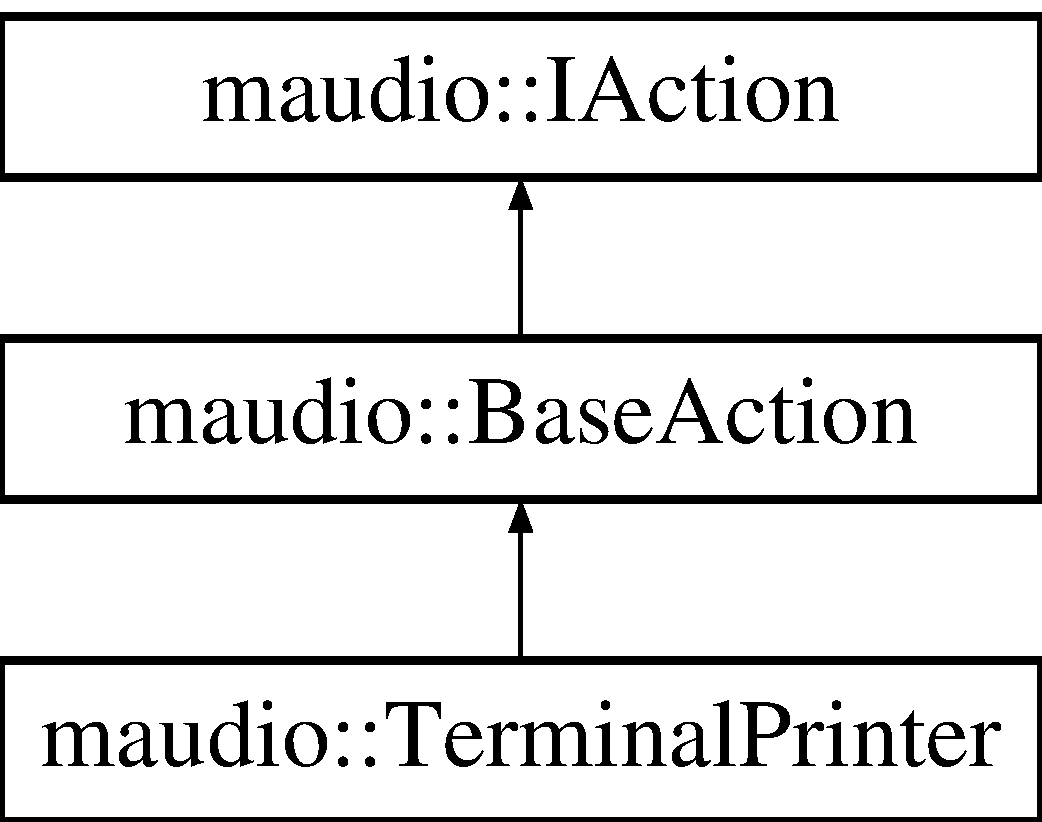
\includegraphics[height=3.000000cm]{classmaudio_1_1TerminalPrinter}
\end{center}
\end{figure}
\subsection*{Public Member Functions}
\begin{DoxyCompactItemize}
\item 
\hyperlink{classmaudio_1_1TerminalPrinter_abd8163dacd3a72c054bcc1a3a0431a32}{Terminal\-Printer} ()
\item 
virtual \hyperlink{classmaudio_1_1TerminalPrinter_a63e4fe3cae91beb77a27461d29f78c98}{$\sim$\-Terminal\-Printer} ()
\item 
virtual \hyperlink{classmaudio_1_1IAudioBuffer}{I\-Audio\-Buffer} $\ast$ \hyperlink{classmaudio_1_1TerminalPrinter_a27f779bcd81b68ffad732a6da669f8fe}{get} (unsigned long pos, unsigned int length) noexcept
\item 
virtual \hyperlink{classmaudio_1_1IAudioInfo}{I\-Audio\-Info} $\ast$ \hyperlink{classmaudio_1_1TerminalPrinter_ae0d8b73356c360bfdd10d32ec829af85}{get\-Info} () noexcept
\item 
virtual int \hyperlink{classmaudio_1_1TerminalPrinter_af895f464f3d51be9d44750e96dabf8f1}{Max\-Inputs} () const 
\item 
virtual bool \hyperlink{classmaudio_1_1TerminalPrinter_a3fdb9711d0d767e9acd0d01b3c7644da}{Has\-Outputs} () const 
\item 
virtual void \hyperlink{classmaudio_1_1TerminalPrinter_a3888206cd622627b441ca00cca6d87e2}{read\-Config} (const \hyperlink{classmaudio_1_1IKeyValueStore}{I\-Key\-Value\-Store} \&conf)
\item 
virtual \hyperlink{classmaudio_1_1IControl}{I\-Control} $\ast$ \hyperlink{classmaudio_1_1TerminalPrinter_acef99a9118ebb6908166d8e97e7bb3e9}{get\-Control} ()
\item 
void \hyperlink{classmaudio_1_1TerminalPrinter_aff5c0d18138794ceea7fd4f4616d5b13}{print} (unsigned long pos)
\end{DoxyCompactItemize}
\subsection*{Additional Inherited Members}


\subsection{Constructor \& Destructor Documentation}
\hypertarget{classmaudio_1_1TerminalPrinter_abd8163dacd3a72c054bcc1a3a0431a32}{\index{maudio\-::\-Terminal\-Printer@{maudio\-::\-Terminal\-Printer}!Terminal\-Printer@{Terminal\-Printer}}
\index{Terminal\-Printer@{Terminal\-Printer}!maudio::TerminalPrinter@{maudio\-::\-Terminal\-Printer}}
\subsubsection[{Terminal\-Printer}]{\setlength{\rightskip}{0pt plus 5cm}maudio\-::\-Terminal\-Printer\-::\-Terminal\-Printer (
\begin{DoxyParamCaption}
{}
\end{DoxyParamCaption}
)}}\label{classmaudio_1_1TerminalPrinter_abd8163dacd3a72c054bcc1a3a0431a32}
\hypertarget{classmaudio_1_1TerminalPrinter_a63e4fe3cae91beb77a27461d29f78c98}{\index{maudio\-::\-Terminal\-Printer@{maudio\-::\-Terminal\-Printer}!$\sim$\-Terminal\-Printer@{$\sim$\-Terminal\-Printer}}
\index{$\sim$\-Terminal\-Printer@{$\sim$\-Terminal\-Printer}!maudio::TerminalPrinter@{maudio\-::\-Terminal\-Printer}}
\subsubsection[{$\sim$\-Terminal\-Printer}]{\setlength{\rightskip}{0pt plus 5cm}maudio\-::\-Terminal\-Printer\-::$\sim$\-Terminal\-Printer (
\begin{DoxyParamCaption}
{}
\end{DoxyParamCaption}
)\hspace{0.3cm}{\ttfamily [virtual]}}}\label{classmaudio_1_1TerminalPrinter_a63e4fe3cae91beb77a27461d29f78c98}


\subsection{Member Function Documentation}
\hypertarget{classmaudio_1_1TerminalPrinter_a27f779bcd81b68ffad732a6da669f8fe}{\index{maudio\-::\-Terminal\-Printer@{maudio\-::\-Terminal\-Printer}!get@{get}}
\index{get@{get}!maudio::TerminalPrinter@{maudio\-::\-Terminal\-Printer}}
\subsubsection[{get}]{\setlength{\rightskip}{0pt plus 5cm}{\bf I\-Audio\-Buffer} $\ast$ maudio\-::\-Terminal\-Printer\-::get (
\begin{DoxyParamCaption}
\item[{unsigned long}]{pos, }
\item[{unsigned int}]{length}
\end{DoxyParamCaption}
)\hspace{0.3cm}{\ttfamily [virtual]}, {\ttfamily [noexcept]}}}\label{classmaudio_1_1TerminalPrinter_a27f779bcd81b68ffad732a6da669f8fe}


Implements \hyperlink{classmaudio_1_1IAction_adcd159456456b1104af6d4f31336fe59}{maudio\-::\-I\-Action}.

\hypertarget{classmaudio_1_1TerminalPrinter_acef99a9118ebb6908166d8e97e7bb3e9}{\index{maudio\-::\-Terminal\-Printer@{maudio\-::\-Terminal\-Printer}!get\-Control@{get\-Control}}
\index{get\-Control@{get\-Control}!maudio::TerminalPrinter@{maudio\-::\-Terminal\-Printer}}
\subsubsection[{get\-Control}]{\setlength{\rightskip}{0pt plus 5cm}{\bf I\-Control} $\ast$ maudio\-::\-Terminal\-Printer\-::get\-Control (
\begin{DoxyParamCaption}
{}
\end{DoxyParamCaption}
)\hspace{0.3cm}{\ttfamily [virtual]}}}\label{classmaudio_1_1TerminalPrinter_acef99a9118ebb6908166d8e97e7bb3e9}


Reimplemented from \hyperlink{classmaudio_1_1BaseAction_a0ecc4f8e47f52d90b0ba7fe2757efe2c}{maudio\-::\-Base\-Action}.

\hypertarget{classmaudio_1_1TerminalPrinter_ae0d8b73356c360bfdd10d32ec829af85}{\index{maudio\-::\-Terminal\-Printer@{maudio\-::\-Terminal\-Printer}!get\-Info@{get\-Info}}
\index{get\-Info@{get\-Info}!maudio::TerminalPrinter@{maudio\-::\-Terminal\-Printer}}
\subsubsection[{get\-Info}]{\setlength{\rightskip}{0pt plus 5cm}{\bf I\-Audio\-Info} $\ast$ maudio\-::\-Terminal\-Printer\-::get\-Info (
\begin{DoxyParamCaption}
{}
\end{DoxyParamCaption}
)\hspace{0.3cm}{\ttfamily [virtual]}, {\ttfamily [noexcept]}}}\label{classmaudio_1_1TerminalPrinter_ae0d8b73356c360bfdd10d32ec829af85}


Implements \hyperlink{classmaudio_1_1IAction_abf9d7d1a4d66fd1b48d946d672bfe7a0}{maudio\-::\-I\-Action}.

\hypertarget{classmaudio_1_1TerminalPrinter_a3fdb9711d0d767e9acd0d01b3c7644da}{\index{maudio\-::\-Terminal\-Printer@{maudio\-::\-Terminal\-Printer}!Has\-Outputs@{Has\-Outputs}}
\index{Has\-Outputs@{Has\-Outputs}!maudio::TerminalPrinter@{maudio\-::\-Terminal\-Printer}}
\subsubsection[{Has\-Outputs}]{\setlength{\rightskip}{0pt plus 5cm}bool maudio\-::\-Terminal\-Printer\-::\-Has\-Outputs (
\begin{DoxyParamCaption}
{}
\end{DoxyParamCaption}
) const\hspace{0.3cm}{\ttfamily [virtual]}}}\label{classmaudio_1_1TerminalPrinter_a3fdb9711d0d767e9acd0d01b3c7644da}


Implements \hyperlink{classmaudio_1_1IAction_a148ec76547dc1ac21e47b4b5d10c152a}{maudio\-::\-I\-Action}.

\hypertarget{classmaudio_1_1TerminalPrinter_af895f464f3d51be9d44750e96dabf8f1}{\index{maudio\-::\-Terminal\-Printer@{maudio\-::\-Terminal\-Printer}!Max\-Inputs@{Max\-Inputs}}
\index{Max\-Inputs@{Max\-Inputs}!maudio::TerminalPrinter@{maudio\-::\-Terminal\-Printer}}
\subsubsection[{Max\-Inputs}]{\setlength{\rightskip}{0pt plus 5cm}int maudio\-::\-Terminal\-Printer\-::\-Max\-Inputs (
\begin{DoxyParamCaption}
{}
\end{DoxyParamCaption}
) const\hspace{0.3cm}{\ttfamily [virtual]}}}\label{classmaudio_1_1TerminalPrinter_af895f464f3d51be9d44750e96dabf8f1}


Implements \hyperlink{classmaudio_1_1IAction_a3c8825e7f38e0de769af7d81ccf6cf5e}{maudio\-::\-I\-Action}.

\hypertarget{classmaudio_1_1TerminalPrinter_aff5c0d18138794ceea7fd4f4616d5b13}{\index{maudio\-::\-Terminal\-Printer@{maudio\-::\-Terminal\-Printer}!print@{print}}
\index{print@{print}!maudio::TerminalPrinter@{maudio\-::\-Terminal\-Printer}}
\subsubsection[{print}]{\setlength{\rightskip}{0pt plus 5cm}void maudio\-::\-Terminal\-Printer\-::print (
\begin{DoxyParamCaption}
\item[{unsigned long}]{pos}
\end{DoxyParamCaption}
)}}\label{classmaudio_1_1TerminalPrinter_aff5c0d18138794ceea7fd4f4616d5b13}
\hypertarget{classmaudio_1_1TerminalPrinter_a3888206cd622627b441ca00cca6d87e2}{\index{maudio\-::\-Terminal\-Printer@{maudio\-::\-Terminal\-Printer}!read\-Config@{read\-Config}}
\index{read\-Config@{read\-Config}!maudio::TerminalPrinter@{maudio\-::\-Terminal\-Printer}}
\subsubsection[{read\-Config}]{\setlength{\rightskip}{0pt plus 5cm}void maudio\-::\-Terminal\-Printer\-::read\-Config (
\begin{DoxyParamCaption}
\item[{const {\bf I\-Key\-Value\-Store} \&}]{conf}
\end{DoxyParamCaption}
)\hspace{0.3cm}{\ttfamily [virtual]}}}\label{classmaudio_1_1TerminalPrinter_a3888206cd622627b441ca00cca6d87e2}


Implements \hyperlink{classmaudio_1_1IAction_a610804d37c46509f3eaa1aebceab7e35}{maudio\-::\-I\-Action}.



The documentation for this class was generated from the following files\-:\begin{DoxyCompactItemize}
\item 
/home/mars/\-Projekte/maudio/src/plugins/include/core/actions/\hyperlink{TerminalPrinter_8hpp}{Terminal\-Printer.\-hpp}\item 
/home/mars/\-Projekte/maudio/src/core/actions/\hyperlink{core_2actions_2TerminalPrinter_8cpp}{Terminal\-Printer.\-cpp}\end{DoxyCompactItemize}

\hypertarget{classTestPlugin}{\section{Test\-Plugin Class Reference}
\label{classTestPlugin}\index{Test\-Plugin@{Test\-Plugin}}
}
Inheritance diagram for Test\-Plugin\-:\begin{figure}[H]
\begin{center}
\leavevmode
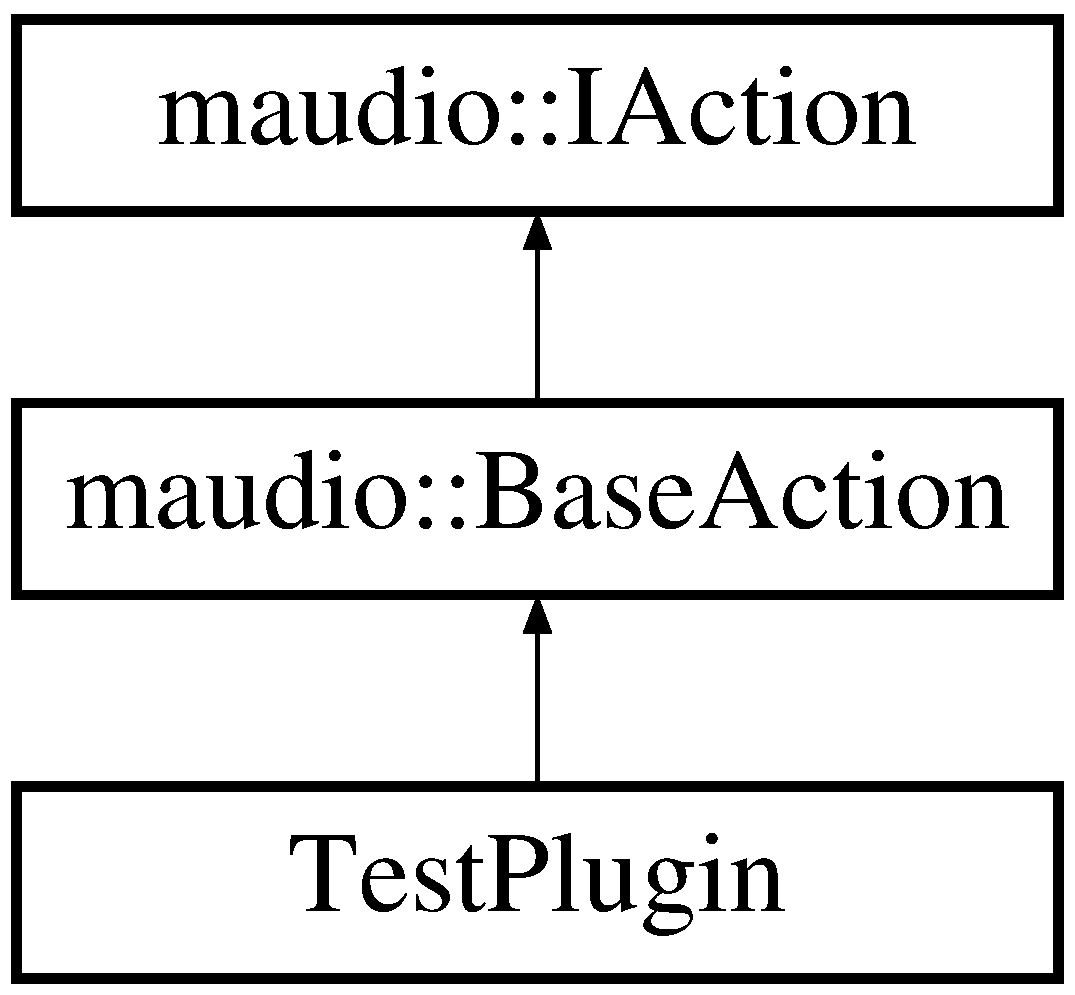
\includegraphics[height=3.000000cm]{classTestPlugin}
\end{center}
\end{figure}
\subsection*{Public Member Functions}
\begin{DoxyCompactItemize}
\item 
\hyperlink{classTestPlugin_a7ba0585e22aa70b5c47cb5811af287a3}{Test\-Plugin} ()
\item 
virtual \hyperlink{classTestPlugin_a6791e3e7343d31cbedd6f46accbf44b3}{$\sim$\-Test\-Plugin} ()
\item 
virtual \hyperlink{classmaudio_1_1IAudioBuffer}{I\-Audio\-Buffer} $\ast$ \hyperlink{classTestPlugin_af45a5a7d4f61db9503d96ecc1c590251}{get} (unsigned long pos, unsigned int length) noexcept
\item 
virtual \hyperlink{classmaudio_1_1IAudioInfo}{I\-Audio\-Info} $\ast$ \hyperlink{classTestPlugin_a07aa6acf3be682c3552c88282a97ceaa}{get\-Info} () noexcept
\item 
virtual int \hyperlink{classTestPlugin_ad4faa8dad53c62e372e5837d8aa59ecb}{Max\-Inputs} () const 
\item 
virtual bool \hyperlink{classTestPlugin_a2eb2cacb18c097fe26cc1a7640eebac3}{Has\-Outputs} () const 
\item 
virtual void \hyperlink{classTestPlugin_acd8d80abecd3967547e401cba0e1b660}{read\-Config} (const \hyperlink{classmaudio_1_1IKeyValueStore}{I\-Key\-Value\-Store} \&conf)
\end{DoxyCompactItemize}
\subsection*{Additional Inherited Members}


\subsection{Constructor \& Destructor Documentation}
\hypertarget{classTestPlugin_a7ba0585e22aa70b5c47cb5811af287a3}{\index{Test\-Plugin@{Test\-Plugin}!Test\-Plugin@{Test\-Plugin}}
\index{Test\-Plugin@{Test\-Plugin}!TestPlugin@{Test\-Plugin}}
\subsubsection[{Test\-Plugin}]{\setlength{\rightskip}{0pt plus 5cm}Test\-Plugin\-::\-Test\-Plugin (
\begin{DoxyParamCaption}
{}
\end{DoxyParamCaption}
)\hspace{0.3cm}{\ttfamily [inline]}}}\label{classTestPlugin_a7ba0585e22aa70b5c47cb5811af287a3}
\hypertarget{classTestPlugin_a6791e3e7343d31cbedd6f46accbf44b3}{\index{Test\-Plugin@{Test\-Plugin}!$\sim$\-Test\-Plugin@{$\sim$\-Test\-Plugin}}
\index{$\sim$\-Test\-Plugin@{$\sim$\-Test\-Plugin}!TestPlugin@{Test\-Plugin}}
\subsubsection[{$\sim$\-Test\-Plugin}]{\setlength{\rightskip}{0pt plus 5cm}virtual Test\-Plugin\-::$\sim$\-Test\-Plugin (
\begin{DoxyParamCaption}
{}
\end{DoxyParamCaption}
)\hspace{0.3cm}{\ttfamily [inline]}, {\ttfamily [virtual]}}}\label{classTestPlugin_a6791e3e7343d31cbedd6f46accbf44b3}


\subsection{Member Function Documentation}
\hypertarget{classTestPlugin_af45a5a7d4f61db9503d96ecc1c590251}{\index{Test\-Plugin@{Test\-Plugin}!get@{get}}
\index{get@{get}!TestPlugin@{Test\-Plugin}}
\subsubsection[{get}]{\setlength{\rightskip}{0pt plus 5cm}virtual {\bf I\-Audio\-Buffer}$\ast$ Test\-Plugin\-::get (
\begin{DoxyParamCaption}
\item[{unsigned long}]{pos, }
\item[{unsigned int}]{length}
\end{DoxyParamCaption}
)\hspace{0.3cm}{\ttfamily [inline]}, {\ttfamily [virtual]}, {\ttfamily [noexcept]}}}\label{classTestPlugin_af45a5a7d4f61db9503d96ecc1c590251}


Implements \hyperlink{classmaudio_1_1IAction_adcd159456456b1104af6d4f31336fe59}{maudio\-::\-I\-Action}.

\hypertarget{classTestPlugin_a07aa6acf3be682c3552c88282a97ceaa}{\index{Test\-Plugin@{Test\-Plugin}!get\-Info@{get\-Info}}
\index{get\-Info@{get\-Info}!TestPlugin@{Test\-Plugin}}
\subsubsection[{get\-Info}]{\setlength{\rightskip}{0pt plus 5cm}virtual {\bf I\-Audio\-Info}$\ast$ Test\-Plugin\-::get\-Info (
\begin{DoxyParamCaption}
{}
\end{DoxyParamCaption}
)\hspace{0.3cm}{\ttfamily [inline]}, {\ttfamily [virtual]}, {\ttfamily [noexcept]}}}\label{classTestPlugin_a07aa6acf3be682c3552c88282a97ceaa}


Implements \hyperlink{classmaudio_1_1IAction_abf9d7d1a4d66fd1b48d946d672bfe7a0}{maudio\-::\-I\-Action}.

\hypertarget{classTestPlugin_a2eb2cacb18c097fe26cc1a7640eebac3}{\index{Test\-Plugin@{Test\-Plugin}!Has\-Outputs@{Has\-Outputs}}
\index{Has\-Outputs@{Has\-Outputs}!TestPlugin@{Test\-Plugin}}
\subsubsection[{Has\-Outputs}]{\setlength{\rightskip}{0pt plus 5cm}virtual bool Test\-Plugin\-::\-Has\-Outputs (
\begin{DoxyParamCaption}
{}
\end{DoxyParamCaption}
) const\hspace{0.3cm}{\ttfamily [inline]}, {\ttfamily [virtual]}}}\label{classTestPlugin_a2eb2cacb18c097fe26cc1a7640eebac3}


Implements \hyperlink{classmaudio_1_1IAction_a148ec76547dc1ac21e47b4b5d10c152a}{maudio\-::\-I\-Action}.

\hypertarget{classTestPlugin_ad4faa8dad53c62e372e5837d8aa59ecb}{\index{Test\-Plugin@{Test\-Plugin}!Max\-Inputs@{Max\-Inputs}}
\index{Max\-Inputs@{Max\-Inputs}!TestPlugin@{Test\-Plugin}}
\subsubsection[{Max\-Inputs}]{\setlength{\rightskip}{0pt plus 5cm}virtual int Test\-Plugin\-::\-Max\-Inputs (
\begin{DoxyParamCaption}
{}
\end{DoxyParamCaption}
) const\hspace{0.3cm}{\ttfamily [inline]}, {\ttfamily [virtual]}}}\label{classTestPlugin_ad4faa8dad53c62e372e5837d8aa59ecb}


Implements \hyperlink{classmaudio_1_1IAction_a3c8825e7f38e0de769af7d81ccf6cf5e}{maudio\-::\-I\-Action}.

\hypertarget{classTestPlugin_acd8d80abecd3967547e401cba0e1b660}{\index{Test\-Plugin@{Test\-Plugin}!read\-Config@{read\-Config}}
\index{read\-Config@{read\-Config}!TestPlugin@{Test\-Plugin}}
\subsubsection[{read\-Config}]{\setlength{\rightskip}{0pt plus 5cm}virtual void Test\-Plugin\-::read\-Config (
\begin{DoxyParamCaption}
\item[{const {\bf I\-Key\-Value\-Store} \&}]{conf}
\end{DoxyParamCaption}
)\hspace{0.3cm}{\ttfamily [inline]}, {\ttfamily [virtual]}}}\label{classTestPlugin_acd8d80abecd3967547e401cba0e1b660}


Implements \hyperlink{classmaudio_1_1IAction_a610804d37c46509f3eaa1aebceab7e35}{maudio\-::\-I\-Action}.



The documentation for this class was generated from the following file\-:\begin{DoxyCompactItemize}
\item 
/home/mars/\-Projekte/maudio/src/plugins/testplugin/\hyperlink{plugin_8cpp}{plugin.\-cpp}\end{DoxyCompactItemize}

\hypertarget{classmaudio_1_1TXTSerializer}{\section{maudio\-:\-:T\-X\-T\-Serializer Class Reference}
\label{classmaudio_1_1TXTSerializer}\index{maudio\-::\-T\-X\-T\-Serializer@{maudio\-::\-T\-X\-T\-Serializer}}
}


{\ttfamily \#include $<$T\-X\-T\-Serializer.\-hpp$>$}

Inheritance diagram for maudio\-:\-:T\-X\-T\-Serializer\-:\begin{figure}[H]
\begin{center}
\leavevmode
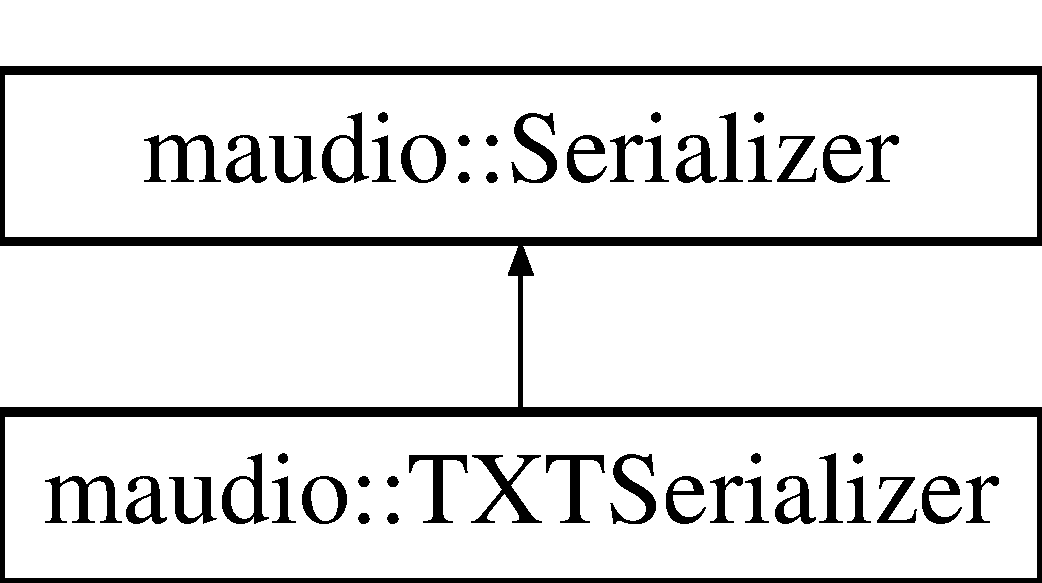
\includegraphics[height=2.000000cm]{classmaudio_1_1TXTSerializer}
\end{center}
\end{figure}
\subsection*{Public Member Functions}
\begin{DoxyCompactItemize}
\item 
\hyperlink{classmaudio_1_1TXTSerializer_a346bdb95f48c621f777c72ff1dbc7763}{T\-X\-T\-Serializer} ()
\item 
\hyperlink{classmaudio_1_1TXTSerializer_a595cb1f5f07fa66b3b678694e0d61c11}{$\sim$\-T\-X\-T\-Serializer} ()
\end{DoxyCompactItemize}


\subsection{Constructor \& Destructor Documentation}
\hypertarget{classmaudio_1_1TXTSerializer_a346bdb95f48c621f777c72ff1dbc7763}{\index{maudio\-::\-T\-X\-T\-Serializer@{maudio\-::\-T\-X\-T\-Serializer}!T\-X\-T\-Serializer@{T\-X\-T\-Serializer}}
\index{T\-X\-T\-Serializer@{T\-X\-T\-Serializer}!maudio::TXTSerializer@{maudio\-::\-T\-X\-T\-Serializer}}
\subsubsection[{T\-X\-T\-Serializer}]{\setlength{\rightskip}{0pt plus 5cm}maudio\-::\-T\-X\-T\-Serializer\-::\-T\-X\-T\-Serializer (
\begin{DoxyParamCaption}
{}
\end{DoxyParamCaption}
)}}\label{classmaudio_1_1TXTSerializer_a346bdb95f48c621f777c72ff1dbc7763}
\hypertarget{classmaudio_1_1TXTSerializer_a595cb1f5f07fa66b3b678694e0d61c11}{\index{maudio\-::\-T\-X\-T\-Serializer@{maudio\-::\-T\-X\-T\-Serializer}!$\sim$\-T\-X\-T\-Serializer@{$\sim$\-T\-X\-T\-Serializer}}
\index{$\sim$\-T\-X\-T\-Serializer@{$\sim$\-T\-X\-T\-Serializer}!maudio::TXTSerializer@{maudio\-::\-T\-X\-T\-Serializer}}
\subsubsection[{$\sim$\-T\-X\-T\-Serializer}]{\setlength{\rightskip}{0pt plus 5cm}maudio\-::\-T\-X\-T\-Serializer\-::$\sim$\-T\-X\-T\-Serializer (
\begin{DoxyParamCaption}
{}
\end{DoxyParamCaption}
)}}\label{classmaudio_1_1TXTSerializer_a595cb1f5f07fa66b3b678694e0d61c11}


The documentation for this class was generated from the following file\-:\begin{DoxyCompactItemize}
\item 
/home/mars/\-Projekte/maudio/src/plugins/include/core/serializer/\hyperlink{TXTSerializer_8hpp}{T\-X\-T\-Serializer.\-hpp}\end{DoxyCompactItemize}

\hypertarget{classmaudio_1_1UniqueID}{\section{maudio\-:\-:Unique\-I\-D Class Reference}
\label{classmaudio_1_1UniqueID}\index{maudio\-::\-Unique\-I\-D@{maudio\-::\-Unique\-I\-D}}
}


{\ttfamily \#include $<$Unique\-I\-D.\-hpp$>$}

Inheritance diagram for maudio\-:\-:Unique\-I\-D\-:\begin{figure}[H]
\begin{center}
\leavevmode
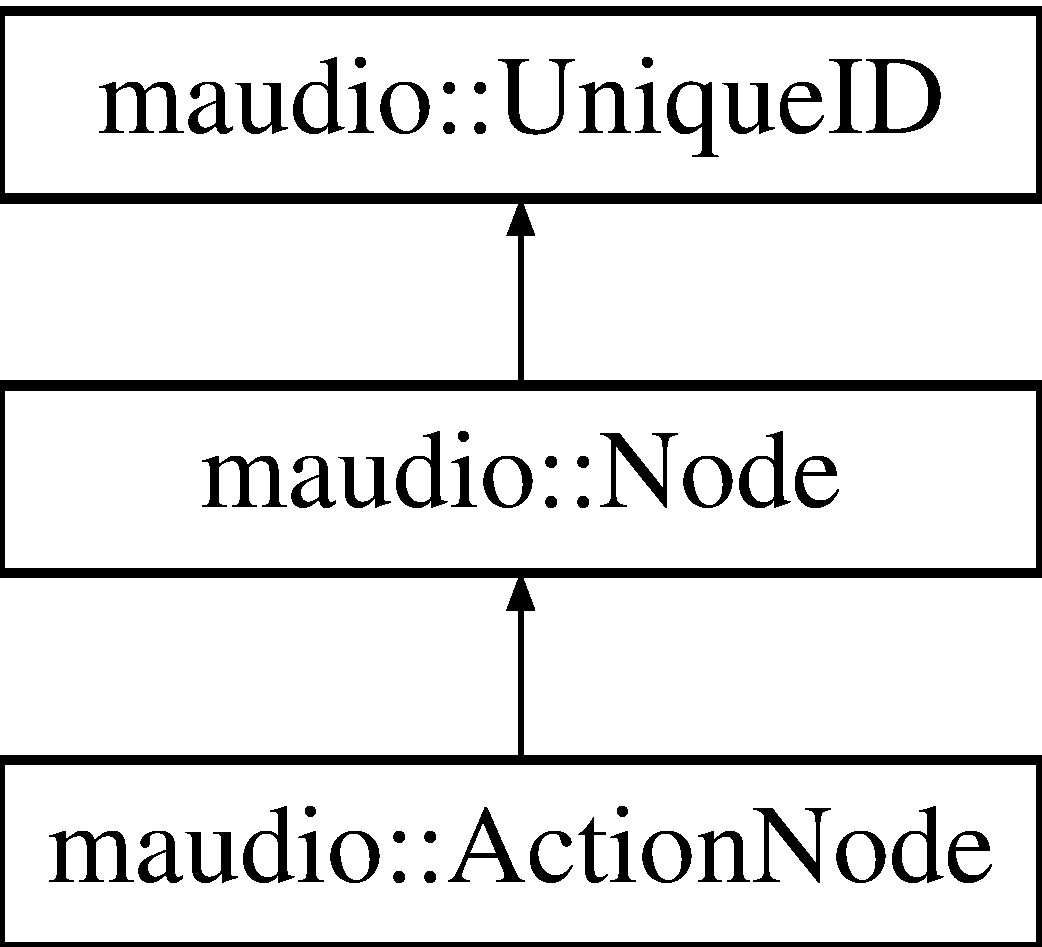
\includegraphics[height=3.000000cm]{classmaudio_1_1UniqueID}
\end{center}
\end{figure}
\subsection*{Public Member Functions}
\begin{DoxyCompactItemize}
\item 
\hyperlink{classmaudio_1_1UniqueID_adb0400fdf981959b43a104258fa73782}{Unique\-I\-D} ()
\item 
const unsigned int \hyperlink{classmaudio_1_1UniqueID_a676302c1b75d6d1dd04171d701aa67d1}{get\-I\-D} ()
\item 
const std\-::string \hyperlink{classmaudio_1_1UniqueID_a5d751bd88057a4e74a7374e0104b1bc7}{get\-I\-D\-Str} ()
\end{DoxyCompactItemize}


\subsection{Constructor \& Destructor Documentation}
\hypertarget{classmaudio_1_1UniqueID_adb0400fdf981959b43a104258fa73782}{\index{maudio\-::\-Unique\-I\-D@{maudio\-::\-Unique\-I\-D}!Unique\-I\-D@{Unique\-I\-D}}
\index{Unique\-I\-D@{Unique\-I\-D}!maudio::UniqueID@{maudio\-::\-Unique\-I\-D}}
\subsubsection[{Unique\-I\-D}]{\setlength{\rightskip}{0pt plus 5cm}maudio\-::\-Unique\-I\-D\-::\-Unique\-I\-D (
\begin{DoxyParamCaption}
{}
\end{DoxyParamCaption}
)}}\label{classmaudio_1_1UniqueID_adb0400fdf981959b43a104258fa73782}


\subsection{Member Function Documentation}
\hypertarget{classmaudio_1_1UniqueID_a676302c1b75d6d1dd04171d701aa67d1}{\index{maudio\-::\-Unique\-I\-D@{maudio\-::\-Unique\-I\-D}!get\-I\-D@{get\-I\-D}}
\index{get\-I\-D@{get\-I\-D}!maudio::UniqueID@{maudio\-::\-Unique\-I\-D}}
\subsubsection[{get\-I\-D}]{\setlength{\rightskip}{0pt plus 5cm}const unsigned int maudio\-::\-Unique\-I\-D\-::get\-I\-D (
\begin{DoxyParamCaption}
{}
\end{DoxyParamCaption}
)}}\label{classmaudio_1_1UniqueID_a676302c1b75d6d1dd04171d701aa67d1}
\hypertarget{classmaudio_1_1UniqueID_a5d751bd88057a4e74a7374e0104b1bc7}{\index{maudio\-::\-Unique\-I\-D@{maudio\-::\-Unique\-I\-D}!get\-I\-D\-Str@{get\-I\-D\-Str}}
\index{get\-I\-D\-Str@{get\-I\-D\-Str}!maudio::UniqueID@{maudio\-::\-Unique\-I\-D}}
\subsubsection[{get\-I\-D\-Str}]{\setlength{\rightskip}{0pt plus 5cm}const std\-::string maudio\-::\-Unique\-I\-D\-::get\-I\-D\-Str (
\begin{DoxyParamCaption}
{}
\end{DoxyParamCaption}
)}}\label{classmaudio_1_1UniqueID_a5d751bd88057a4e74a7374e0104b1bc7}


The documentation for this class was generated from the following files\-:\begin{DoxyCompactItemize}
\item 
/home/mars/\-Projekte/maudio/src/plugins/include/core/util/\hyperlink{UniqueID_8hpp}{Unique\-I\-D.\-hpp}\item 
/home/mars/\-Projekte/maudio/src/core/util/\hyperlink{core_2util_2UniqueID_8cpp}{Unique\-I\-D.\-cpp}\end{DoxyCompactItemize}

\chapter{File Documentation}
\hypertarget{core_2actions_2BaseAction_8cpp}{\section{/home/mars/\-Projekte/maudio/src/core/actions/\-Base\-Action.cpp File Reference}
\label{core_2actions_2BaseAction_8cpp}\index{/home/mars/\-Projekte/maudio/src/core/actions/\-Base\-Action.\-cpp@{/home/mars/\-Projekte/maudio/src/core/actions/\-Base\-Action.\-cpp}}
}
{\ttfamily \#include \char`\"{}core/actions/\-Base\-Action.\-hpp\char`\"{}}\\*
\subsection*{Namespaces}
\begin{DoxyCompactItemize}
\item 
\hyperlink{namespacemaudio}{maudio}
\end{DoxyCompactItemize}

\hypertarget{plugins_2include_2core_2actions_2BaseAction_8cpp}{\section{/home/mars/\-Projekte/maudio/src/plugins/include/core/actions/\-Base\-Action.cpp File Reference}
\label{plugins_2include_2core_2actions_2BaseAction_8cpp}\index{/home/mars/\-Projekte/maudio/src/plugins/include/core/actions/\-Base\-Action.\-cpp@{/home/mars/\-Projekte/maudio/src/plugins/include/core/actions/\-Base\-Action.\-cpp}}
}
{\ttfamily \#include \char`\"{}core/actions/\-Base\-Action.\-hpp\char`\"{}}\\*
\subsection*{Namespaces}
\begin{DoxyCompactItemize}
\item 
\hyperlink{namespacemaudio}{maudio}
\end{DoxyCompactItemize}

\hypertarget{core_2actions_2SinusGenerator_8cpp}{\section{/home/mars/\-Projekte/maudio/src/core/actions/\-Sinus\-Generator.cpp File Reference}
\label{core_2actions_2SinusGenerator_8cpp}\index{/home/mars/\-Projekte/maudio/src/core/actions/\-Sinus\-Generator.\-cpp@{/home/mars/\-Projekte/maudio/src/core/actions/\-Sinus\-Generator.\-cpp}}
}
{\ttfamily \#include \char`\"{}core/actions/\-Sinus\-Generator.\-hpp\char`\"{}}\\*
{\ttfamily \#include \char`\"{}core/audiodata/\-Audio\-Buffer.\-hpp\char`\"{}}\\*
{\ttfamily \#include \char`\"{}core/util/\-Audio\-Exception.\-hpp\char`\"{}}\\*
{\ttfamily \#include \char`\"{}core/util/\-Util.\-hpp\char`\"{}}\\*
{\ttfamily \#include $<$cmath$>$}\\*
\subsection*{Namespaces}
\begin{DoxyCompactItemize}
\item 
\hyperlink{namespacemaudio}{maudio}
\end{DoxyCompactItemize}

\hypertarget{core_2deprecated_2audiosource_2SinusGenerator_8cpp}{\section{/home/mars/\-Projekte/maudio/src/core/deprecated/audiosource/\-Sinus\-Generator.cpp File Reference}
\label{core_2deprecated_2audiosource_2SinusGenerator_8cpp}\index{/home/mars/\-Projekte/maudio/src/core/deprecated/audiosource/\-Sinus\-Generator.\-cpp@{/home/mars/\-Projekte/maudio/src/core/deprecated/audiosource/\-Sinus\-Generator.\-cpp}}
}
{\ttfamily \#include \char`\"{}core/audiosource/\-Sinus\-Generator.\-hpp\char`\"{}}\\*
{\ttfamily \#include \char`\"{}core/util/\-Audio\-Exception.\-hpp\char`\"{}}\\*
{\ttfamily \#include \char`\"{}core/util/\-Util.\-hpp\char`\"{}}\\*
{\ttfamily \#include $<$cmath$>$}\\*
\subsection*{Namespaces}
\begin{DoxyCompactItemize}
\item 
\hyperlink{namespacemaudio}{maudio}
\end{DoxyCompactItemize}

\hypertarget{plugins_2include_2core_2actions_2SinusGenerator_8cpp}{\section{/home/mars/\-Projekte/maudio/src/plugins/include/core/actions/\-Sinus\-Generator.cpp File Reference}
\label{plugins_2include_2core_2actions_2SinusGenerator_8cpp}\index{/home/mars/\-Projekte/maudio/src/plugins/include/core/actions/\-Sinus\-Generator.\-cpp@{/home/mars/\-Projekte/maudio/src/plugins/include/core/actions/\-Sinus\-Generator.\-cpp}}
}
{\ttfamily \#include \char`\"{}core/actions/\-Sinus\-Generator.\-hpp\char`\"{}}\\*
{\ttfamily \#include \char`\"{}core/audiodata/\-Audio\-Buffer.\-hpp\char`\"{}}\\*
{\ttfamily \#include \char`\"{}core/util/\-Audio\-Exception.\-hpp\char`\"{}}\\*
{\ttfamily \#include \char`\"{}core/util/\-Util.\-hpp\char`\"{}}\\*
{\ttfamily \#include $<$cmath$>$}\\*
\subsection*{Namespaces}
\begin{DoxyCompactItemize}
\item 
\hyperlink{namespacemaudio}{maudio}
\end{DoxyCompactItemize}

\hypertarget{core_2actions_2TerminalPrinter_8cpp}{\section{/home/mars/\-Projekte/maudio/src/core/actions/\-Terminal\-Printer.cpp File Reference}
\label{core_2actions_2TerminalPrinter_8cpp}\index{/home/mars/\-Projekte/maudio/src/core/actions/\-Terminal\-Printer.\-cpp@{/home/mars/\-Projekte/maudio/src/core/actions/\-Terminal\-Printer.\-cpp}}
}
{\ttfamily \#include \char`\"{}core/actions/\-Terminal\-Printer.\-hpp\char`\"{}}\\*
{\ttfamily \#include \char`\"{}core/util/\-Util.\-hpp\char`\"{}}\\*
{\ttfamily \#include \char`\"{}core/util/\-Audio\-Exception.\-hpp\char`\"{}}\\*
{\ttfamily \#include \char`\"{}core/util/action\-\_\-ptr.\-hpp\char`\"{}}\\*
{\ttfamily \#include $<$iostream$>$}\\*
{\ttfamily \#include $<$cstring$>$}\\*
\subsection*{Namespaces}
\begin{DoxyCompactItemize}
\item 
\hyperlink{namespacemaudio}{maudio}
\end{DoxyCompactItemize}

\hypertarget{core_2deprecated_2audiosink_2TerminalPrinter_8cpp}{\section{/home/mars/\-Projekte/maudio/src/core/deprecated/audiosink/\-Terminal\-Printer.cpp File Reference}
\label{core_2deprecated_2audiosink_2TerminalPrinter_8cpp}\index{/home/mars/\-Projekte/maudio/src/core/deprecated/audiosink/\-Terminal\-Printer.\-cpp@{/home/mars/\-Projekte/maudio/src/core/deprecated/audiosink/\-Terminal\-Printer.\-cpp}}
}
{\ttfamily \#include \char`\"{}core/audiosink/\-Terminal\-Printer.\-hpp\char`\"{}}\\*
{\ttfamily \#include \char`\"{}core/util/\-Audio\-Exception.\-hpp\char`\"{}}\\*
{\ttfamily \#include $<$iostream$>$}\\*
\subsection*{Namespaces}
\begin{DoxyCompactItemize}
\item 
\hyperlink{namespacemaudio}{maudio}
\end{DoxyCompactItemize}

\hypertarget{plugins_2include_2core_2actions_2TerminalPrinter_8cpp}{\section{/home/mars/\-Projekte/maudio/src/plugins/include/core/actions/\-Terminal\-Printer.cpp File Reference}
\label{plugins_2include_2core_2actions_2TerminalPrinter_8cpp}\index{/home/mars/\-Projekte/maudio/src/plugins/include/core/actions/\-Terminal\-Printer.\-cpp@{/home/mars/\-Projekte/maudio/src/plugins/include/core/actions/\-Terminal\-Printer.\-cpp}}
}
{\ttfamily \#include \char`\"{}core/actions/\-Terminal\-Printer.\-hpp\char`\"{}}\\*
{\ttfamily \#include \char`\"{}core/util/\-Util.\-hpp\char`\"{}}\\*
{\ttfamily \#include \char`\"{}core/util/\-Audio\-Exception.\-hpp\char`\"{}}\\*
{\ttfamily \#include \char`\"{}core/util/action\-\_\-ptr.\-hpp\char`\"{}}\\*
{\ttfamily \#include $<$iostream$>$}\\*
{\ttfamily \#include $<$cstring$>$}\\*
\subsection*{Namespaces}
\begin{DoxyCompactItemize}
\item 
\hyperlink{namespacemaudio}{maudio}
\end{DoxyCompactItemize}

\hypertarget{core_2audiodata_2AudioBuffer_8cpp}{\section{/home/mars/\-Projekte/maudio/src/core/audiodata/\-Audio\-Buffer.cpp File Reference}
\label{core_2audiodata_2AudioBuffer_8cpp}\index{/home/mars/\-Projekte/maudio/src/core/audiodata/\-Audio\-Buffer.\-cpp@{/home/mars/\-Projekte/maudio/src/core/audiodata/\-Audio\-Buffer.\-cpp}}
}
{\ttfamily \#include \char`\"{}core/audiodata/\-Audio\-Buffer.\-hpp\char`\"{}}\\*
{\ttfamily \#include \char`\"{}core/util/\-Audio\-Exception.\-hpp\char`\"{}}\\*
\subsection*{Namespaces}
\begin{DoxyCompactItemize}
\item 
\hyperlink{namespacemaudio}{maudio}
\end{DoxyCompactItemize}

\hypertarget{plugins_2include_2core_2audiodata_2AudioBuffer_8cpp}{\section{/home/mars/\-Projekte/maudio/src/plugins/include/core/audiodata/\-Audio\-Buffer.cpp File Reference}
\label{plugins_2include_2core_2audiodata_2AudioBuffer_8cpp}\index{/home/mars/\-Projekte/maudio/src/plugins/include/core/audiodata/\-Audio\-Buffer.\-cpp@{/home/mars/\-Projekte/maudio/src/plugins/include/core/audiodata/\-Audio\-Buffer.\-cpp}}
}
{\ttfamily \#include \char`\"{}core/audiodata/\-Audio\-Buffer.\-hpp\char`\"{}}\\*
{\ttfamily \#include \char`\"{}core/util/\-Audio\-Exception.\-hpp\char`\"{}}\\*
\subsection*{Namespaces}
\begin{DoxyCompactItemize}
\item 
\hyperlink{namespacemaudio}{maudio}
\end{DoxyCompactItemize}

\hypertarget{core_2audiodata_2AudioQueue_8cpp}{\section{/home/mars/\-Projekte/maudio/src/core/audiodata/\-Audio\-Queue.cpp File Reference}
\label{core_2audiodata_2AudioQueue_8cpp}\index{/home/mars/\-Projekte/maudio/src/core/audiodata/\-Audio\-Queue.\-cpp@{/home/mars/\-Projekte/maudio/src/core/audiodata/\-Audio\-Queue.\-cpp}}
}
{\ttfamily \#include \char`\"{}core/audiodata/\-Audio\-Queue.\-hpp\char`\"{}}\\*
{\ttfamily \#include $<$iostream$>$}\\*
{\ttfamily \#include $<$cmath$>$}\\*
\subsection*{Namespaces}
\begin{DoxyCompactItemize}
\item 
\hyperlink{namespacemaudio}{maudio}
\end{DoxyCompactItemize}

\hypertarget{plugins_2include_2core_2audiodata_2AudioQueue_8cpp}{\section{/home/mars/\-Projekte/maudio/src/plugins/include/core/audiodata/\-Audio\-Queue.cpp File Reference}
\label{plugins_2include_2core_2audiodata_2AudioQueue_8cpp}\index{/home/mars/\-Projekte/maudio/src/plugins/include/core/audiodata/\-Audio\-Queue.\-cpp@{/home/mars/\-Projekte/maudio/src/plugins/include/core/audiodata/\-Audio\-Queue.\-cpp}}
}
{\ttfamily \#include \char`\"{}core/audiodata/\-Audio\-Queue.\-hpp\char`\"{}}\\*
{\ttfamily \#include $<$iostream$>$}\\*
{\ttfamily \#include $<$cmath$>$}\\*
\subsection*{Namespaces}
\begin{DoxyCompactItemize}
\item 
\hyperlink{namespacemaudio}{maudio}
\end{DoxyCompactItemize}

\hypertarget{core_2audiodata_2Sample_8cpp}{\section{/home/mars/\-Projekte/maudio/src/core/audiodata/\-Sample.cpp File Reference}
\label{core_2audiodata_2Sample_8cpp}\index{/home/mars/\-Projekte/maudio/src/core/audiodata/\-Sample.\-cpp@{/home/mars/\-Projekte/maudio/src/core/audiodata/\-Sample.\-cpp}}
}
{\ttfamily \#include \char`\"{}core/audiodata/\-Sample.\-hpp\char`\"{}}\\*
{\ttfamily \#include \char`\"{}core/util/\-Audio\-Exception.\-hpp\char`\"{}}\\*
\subsection*{Namespaces}
\begin{DoxyCompactItemize}
\item 
\hyperlink{namespacemaudio}{maudio}
\end{DoxyCompactItemize}

\hypertarget{plugins_2include_2core_2audiodata_2Sample_8cpp}{\section{/home/mars/\-Projekte/maudio/src/plugins/include/core/audiodata/\-Sample.cpp File Reference}
\label{plugins_2include_2core_2audiodata_2Sample_8cpp}\index{/home/mars/\-Projekte/maudio/src/plugins/include/core/audiodata/\-Sample.\-cpp@{/home/mars/\-Projekte/maudio/src/plugins/include/core/audiodata/\-Sample.\-cpp}}
}
{\ttfamily \#include \char`\"{}core/audiodata/\-Sample.\-hpp\char`\"{}}\\*
{\ttfamily \#include \char`\"{}core/util/\-Audio\-Exception.\-hpp\char`\"{}}\\*
\subsection*{Namespaces}
\begin{DoxyCompactItemize}
\item 
\hyperlink{namespacemaudio}{maudio}
\end{DoxyCompactItemize}

\hypertarget{BaseAudioSink_8cpp}{\section{/home/mars/\-Projekte/maudio/src/core/deprecated/audiosink/\-Base\-Audio\-Sink.cpp File Reference}
\label{BaseAudioSink_8cpp}\index{/home/mars/\-Projekte/maudio/src/core/deprecated/audiosink/\-Base\-Audio\-Sink.\-cpp@{/home/mars/\-Projekte/maudio/src/core/deprecated/audiosink/\-Base\-Audio\-Sink.\-cpp}}
}
{\ttfamily \#include \char`\"{}core/audiosink/\-Base\-Audio\-Sink.\-hpp\char`\"{}}\\*
{\ttfamily \#include \char`\"{}core/util/\-Audio\-Exception.\-hpp\char`\"{}}\\*
{\ttfamily \#include $<$iostream$>$}\\*
\subsection*{Namespaces}
\begin{DoxyCompactItemize}
\item 
\hyperlink{namespacemaudio}{maudio}
\end{DoxyCompactItemize}

\hypertarget{Performance_8cpp}{\section{/home/mars/\-Projekte/maudio/src/core/deprecated/audiosink/\-Performance.cpp File Reference}
\label{Performance_8cpp}\index{/home/mars/\-Projekte/maudio/src/core/deprecated/audiosink/\-Performance.\-cpp@{/home/mars/\-Projekte/maudio/src/core/deprecated/audiosink/\-Performance.\-cpp}}
}
{\ttfamily \#include \char`\"{}core/audiosink/\-Performance.\-hpp\char`\"{}}\\*
{\ttfamily \#include \char`\"{}core/util/\-Audio\-Exception.\-hpp\char`\"{}}\\*
{\ttfamily \#include $<$iostream$>$}\\*
{\ttfamily \#include $<$chrono$>$}\\*
\subsection*{Namespaces}
\begin{DoxyCompactItemize}
\item 
\hyperlink{namespacemaudio}{maudio}
\end{DoxyCompactItemize}

\hypertarget{BaseAudioSource_8cpp}{\section{/home/mars/\-Projekte/maudio/src/core/deprecated/audiosource/\-Base\-Audio\-Source.cpp File Reference}
\label{BaseAudioSource_8cpp}\index{/home/mars/\-Projekte/maudio/src/core/deprecated/audiosource/\-Base\-Audio\-Source.\-cpp@{/home/mars/\-Projekte/maudio/src/core/deprecated/audiosource/\-Base\-Audio\-Source.\-cpp}}
}
{\ttfamily \#include \char`\"{}core/audiosource/\-Base\-Audio\-Source.\-hpp\char`\"{}}\\*
\subsection*{Namespaces}
\begin{DoxyCompactItemize}
\item 
\hyperlink{namespacemaudio}{maudio}
\end{DoxyCompactItemize}

\hypertarget{BaseManipulator_8cpp}{\section{/home/mars/\-Projekte/maudio/src/core/deprecated/manipulator/\-Base\-Manipulator.cpp File Reference}
\label{BaseManipulator_8cpp}\index{/home/mars/\-Projekte/maudio/src/core/deprecated/manipulator/\-Base\-Manipulator.\-cpp@{/home/mars/\-Projekte/maudio/src/core/deprecated/manipulator/\-Base\-Manipulator.\-cpp}}
}
{\ttfamily \#include \char`\"{}core/manipulator/\-Base\-Manipulator.\-hpp\char`\"{}}\\*
\subsection*{Namespaces}
\begin{DoxyCompactItemize}
\item 
\hyperlink{namespacemaudio}{maudio}
\end{DoxyCompactItemize}

\hypertarget{Mixer_8cpp}{\section{/home/mars/\-Projekte/maudio/src/core/deprecated/manipulator/\-Mixer.cpp File Reference}
\label{Mixer_8cpp}\index{/home/mars/\-Projekte/maudio/src/core/deprecated/manipulator/\-Mixer.\-cpp@{/home/mars/\-Projekte/maudio/src/core/deprecated/manipulator/\-Mixer.\-cpp}}
}
{\ttfamily \#include \char`\"{}core/manipulator/\-Mixer.\-hpp\char`\"{}}\\*
\subsection*{Namespaces}
\begin{DoxyCompactItemize}
\item 
\hyperlink{namespacemaudio}{maudio}
\end{DoxyCompactItemize}

\hypertarget{Resampler_8cpp}{\section{/home/mars/\-Projekte/maudio/src/core/deprecated/manipulator/\-Resampler.cpp File Reference}
\label{Resampler_8cpp}\index{/home/mars/\-Projekte/maudio/src/core/deprecated/manipulator/\-Resampler.\-cpp@{/home/mars/\-Projekte/maudio/src/core/deprecated/manipulator/\-Resampler.\-cpp}}
}
{\ttfamily \#include \char`\"{}core/manipulator/\-Resampler.\-hpp\char`\"{}}\\*
{\ttfamily \#include $<$cmath$>$}\\*
{\ttfamily \#include $<$iostream$>$}\\*
\subsection*{Namespaces}
\begin{DoxyCompactItemize}
\item 
\hyperlink{namespacemaudio}{maudio}
\end{DoxyCompactItemize}

\hypertarget{core_2node_2ActionNode_8cpp}{\section{/home/mars/\-Projekte/maudio/src/core/node/\-Action\-Node.cpp File Reference}
\label{core_2node_2ActionNode_8cpp}\index{/home/mars/\-Projekte/maudio/src/core/node/\-Action\-Node.\-cpp@{/home/mars/\-Projekte/maudio/src/core/node/\-Action\-Node.\-cpp}}
}
{\ttfamily \#include \char`\"{}core/node/\-Action\-Node.\-hpp\char`\"{}}\\*
{\ttfamily \#include \char`\"{}core/util/\-Audio\-Exception.\-hpp\char`\"{}}\\*
\subsection*{Namespaces}
\begin{DoxyCompactItemize}
\item 
\hyperlink{namespacemaudio}{maudio}
\end{DoxyCompactItemize}

\hypertarget{plugins_2include_2core_2node_2ActionNode_8cpp}{\section{/home/mars/\-Projekte/maudio/src/plugins/include/core/node/\-Action\-Node.cpp File Reference}
\label{plugins_2include_2core_2node_2ActionNode_8cpp}\index{/home/mars/\-Projekte/maudio/src/plugins/include/core/node/\-Action\-Node.\-cpp@{/home/mars/\-Projekte/maudio/src/plugins/include/core/node/\-Action\-Node.\-cpp}}
}
{\ttfamily \#include \char`\"{}core/node/\-Action\-Node.\-hpp\char`\"{}}\\*
{\ttfamily \#include \char`\"{}core/util/\-Audio\-Exception.\-hpp\char`\"{}}\\*
\subsection*{Namespaces}
\begin{DoxyCompactItemize}
\item 
\hyperlink{namespacemaudio}{maudio}
\end{DoxyCompactItemize}

\hypertarget{core_2node_2Node_8cpp}{\section{/home/mars/\-Projekte/maudio/src/core/node/\-Node.cpp File Reference}
\label{core_2node_2Node_8cpp}\index{/home/mars/\-Projekte/maudio/src/core/node/\-Node.\-cpp@{/home/mars/\-Projekte/maudio/src/core/node/\-Node.\-cpp}}
}
{\ttfamily \#include \char`\"{}core/node/\-Node.\-hpp\char`\"{}}\\*
{\ttfamily \#include \char`\"{}core/util/\-Audio\-Exception.\-hpp\char`\"{}}\\*
\subsection*{Namespaces}
\begin{DoxyCompactItemize}
\item 
\hyperlink{namespacemaudio}{maudio}
\end{DoxyCompactItemize}

\hypertarget{plugins_2include_2core_2node_2Node_8cpp}{\section{/home/mars/\-Projekte/maudio/src/plugins/include/core/node/\-Node.cpp File Reference}
\label{plugins_2include_2core_2node_2Node_8cpp}\index{/home/mars/\-Projekte/maudio/src/plugins/include/core/node/\-Node.\-cpp@{/home/mars/\-Projekte/maudio/src/plugins/include/core/node/\-Node.\-cpp}}
}
{\ttfamily \#include \char`\"{}core/node/\-Node.\-hpp\char`\"{}}\\*
{\ttfamily \#include \char`\"{}core/util/\-Audio\-Exception.\-hpp\char`\"{}}\\*
\subsection*{Namespaces}
\begin{DoxyCompactItemize}
\item 
\hyperlink{namespacemaudio}{maudio}
\end{DoxyCompactItemize}

\hypertarget{core_2node_2Scene_8cpp}{\section{/home/mars/\-Projekte/maudio/src/core/node/\-Scene.cpp File Reference}
\label{core_2node_2Scene_8cpp}\index{/home/mars/\-Projekte/maudio/src/core/node/\-Scene.\-cpp@{/home/mars/\-Projekte/maudio/src/core/node/\-Scene.\-cpp}}
}
{\ttfamily \#include \char`\"{}core/node/\-Node.\-hpp\char`\"{}}\\*
{\ttfamily \#include \char`\"{}core/util/\-Audio\-Exception.\-hpp\char`\"{}}\\*
\subsection*{Namespaces}
\begin{DoxyCompactItemize}
\item 
\hyperlink{namespacemaudio}{maudio}
\end{DoxyCompactItemize}

\hypertarget{plugins_2include_2core_2node_2Scene_8cpp}{\section{/home/mars/\-Projekte/maudio/src/plugins/include/core/node/\-Scene.cpp File Reference}
\label{plugins_2include_2core_2node_2Scene_8cpp}\index{/home/mars/\-Projekte/maudio/src/plugins/include/core/node/\-Scene.\-cpp@{/home/mars/\-Projekte/maudio/src/plugins/include/core/node/\-Scene.\-cpp}}
}
{\ttfamily \#include \char`\"{}core/node/\-Node.\-hpp\char`\"{}}\\*
{\ttfamily \#include \char`\"{}core/util/\-Audio\-Exception.\-hpp\char`\"{}}\\*
\subsection*{Namespaces}
\begin{DoxyCompactItemize}
\item 
\hyperlink{namespacemaudio}{maudio}
\end{DoxyCompactItemize}

\hypertarget{PluginManager_8cpp}{\section{/home/mars/\-Projekte/maudio/src/core/pluginmanager/\-Plugin\-Manager.cpp File Reference}
\label{PluginManager_8cpp}\index{/home/mars/\-Projekte/maudio/src/core/pluginmanager/\-Plugin\-Manager.\-cpp@{/home/mars/\-Projekte/maudio/src/core/pluginmanager/\-Plugin\-Manager.\-cpp}}
}

\hypertarget{core_2property_2PropertyManager_8cpp}{\section{/home/mars/\-Projekte/maudio/src/core/property/\-Property\-Manager.cpp File Reference}
\label{core_2property_2PropertyManager_8cpp}\index{/home/mars/\-Projekte/maudio/src/core/property/\-Property\-Manager.\-cpp@{/home/mars/\-Projekte/maudio/src/core/property/\-Property\-Manager.\-cpp}}
}
{\ttfamily \#include \char`\"{}core/property/\-Property\-Manager.\-hpp\char`\"{}}\\*
{\ttfamily \#include $<$cstddef$>$}\\*
\subsection*{Namespaces}
\begin{DoxyCompactItemize}
\item 
\hyperlink{namespacemaudio}{maudio}
\end{DoxyCompactItemize}

\hypertarget{plugins_2include_2core_2property_2PropertyManager_8cpp}{\section{/home/mars/\-Projekte/maudio/src/plugins/include/core/property/\-Property\-Manager.cpp File Reference}
\label{plugins_2include_2core_2property_2PropertyManager_8cpp}\index{/home/mars/\-Projekte/maudio/src/plugins/include/core/property/\-Property\-Manager.\-cpp@{/home/mars/\-Projekte/maudio/src/plugins/include/core/property/\-Property\-Manager.\-cpp}}
}
{\ttfamily \#include \char`\"{}core/property/\-Property\-Manager.\-hpp\char`\"{}}\\*
{\ttfamily \#include $<$cstddef$>$}\\*
\subsection*{Namespaces}
\begin{DoxyCompactItemize}
\item 
\hyperlink{namespacemaudio}{maudio}
\end{DoxyCompactItemize}

\hypertarget{core_2property_2SimpleKeyableProperty_8cpp}{\section{/home/mars/\-Projekte/maudio/src/core/property/\-Simple\-Keyable\-Property.cpp File Reference}
\label{core_2property_2SimpleKeyableProperty_8cpp}\index{/home/mars/\-Projekte/maudio/src/core/property/\-Simple\-Keyable\-Property.\-cpp@{/home/mars/\-Projekte/maudio/src/core/property/\-Simple\-Keyable\-Property.\-cpp}}
}
{\ttfamily \#include \char`\"{}core/property/\-Simple\-Keyable\-Property.\-hpp\char`\"{}}\\*
\subsection*{Namespaces}
\begin{DoxyCompactItemize}
\item 
\hyperlink{namespacemaudio}{maudio}
\end{DoxyCompactItemize}

\hypertarget{plugins_2include_2core_2property_2SimpleKeyableProperty_8cpp}{\section{/home/mars/\-Projekte/maudio/src/plugins/include/core/property/\-Simple\-Keyable\-Property.cpp File Reference}
\label{plugins_2include_2core_2property_2SimpleKeyableProperty_8cpp}\index{/home/mars/\-Projekte/maudio/src/plugins/include/core/property/\-Simple\-Keyable\-Property.\-cpp@{/home/mars/\-Projekte/maudio/src/plugins/include/core/property/\-Simple\-Keyable\-Property.\-cpp}}
}
{\ttfamily \#include \char`\"{}core/property/\-Simple\-Keyable\-Property.\-hpp\char`\"{}}\\*
\subsection*{Namespaces}
\begin{DoxyCompactItemize}
\item 
\hyperlink{namespacemaudio}{maudio}
\end{DoxyCompactItemize}

\hypertarget{core_2property_2SimpleProperty_8cpp}{\section{/home/mars/\-Projekte/maudio/src/core/property/\-Simple\-Property.cpp File Reference}
\label{core_2property_2SimpleProperty_8cpp}\index{/home/mars/\-Projekte/maudio/src/core/property/\-Simple\-Property.\-cpp@{/home/mars/\-Projekte/maudio/src/core/property/\-Simple\-Property.\-cpp}}
}
{\ttfamily \#include \char`\"{}core/property/\-Simple\-Property.\-hpp\char`\"{}}\\*
{\ttfamily \#include $<$exception$>$}\\*
{\ttfamily \#include $<$limits$>$}\\*
\subsection*{Namespaces}
\begin{DoxyCompactItemize}
\item 
\hyperlink{namespacemaudio}{maudio}
\end{DoxyCompactItemize}

\hypertarget{plugins_2include_2core_2property_2SimpleProperty_8cpp}{\section{/home/mars/\-Projekte/maudio/src/plugins/include/core/property/\-Simple\-Property.cpp File Reference}
\label{plugins_2include_2core_2property_2SimpleProperty_8cpp}\index{/home/mars/\-Projekte/maudio/src/plugins/include/core/property/\-Simple\-Property.\-cpp@{/home/mars/\-Projekte/maudio/src/plugins/include/core/property/\-Simple\-Property.\-cpp}}
}
{\ttfamily \#include \char`\"{}core/property/\-Simple\-Property.\-hpp\char`\"{}}\\*
{\ttfamily \#include $<$exception$>$}\\*
{\ttfamily \#include $<$limits$>$}\\*
\subsection*{Namespaces}
\begin{DoxyCompactItemize}
\item 
\hyperlink{namespacemaudio}{maudio}
\end{DoxyCompactItemize}

\hypertarget{core_2serializer_2SerializerStore_8cpp}{\section{/home/mars/\-Projekte/maudio/src/core/serializer/\-Serializer\-Store.cpp File Reference}
\label{core_2serializer_2SerializerStore_8cpp}\index{/home/mars/\-Projekte/maudio/src/core/serializer/\-Serializer\-Store.\-cpp@{/home/mars/\-Projekte/maudio/src/core/serializer/\-Serializer\-Store.\-cpp}}
}
{\ttfamily \#include \char`\"{}core/serializer/\-Serializer\-Store.\-hpp\char`\"{}}\\*
\subsection*{Namespaces}
\begin{DoxyCompactItemize}
\item 
\hyperlink{namespacemaudio}{maudio}
\end{DoxyCompactItemize}

\hypertarget{plugins_2include_2core_2serializer_2SerializerStore_8cpp}{\section{/home/mars/\-Projekte/maudio/src/plugins/include/core/serializer/\-Serializer\-Store.cpp File Reference}
\label{plugins_2include_2core_2serializer_2SerializerStore_8cpp}\index{/home/mars/\-Projekte/maudio/src/plugins/include/core/serializer/\-Serializer\-Store.\-cpp@{/home/mars/\-Projekte/maudio/src/plugins/include/core/serializer/\-Serializer\-Store.\-cpp}}
}
{\ttfamily \#include \char`\"{}core/serializer/\-Serializer\-Store.\-hpp\char`\"{}}\\*
\subsection*{Namespaces}
\begin{DoxyCompactItemize}
\item 
\hyperlink{namespacemaudio}{maudio}
\end{DoxyCompactItemize}

\hypertarget{core_2serializer_2TXTSerializer_8cpp}{\section{/home/mars/\-Projekte/maudio/src/core/serializer/\-T\-X\-T\-Serializer.cpp File Reference}
\label{core_2serializer_2TXTSerializer_8cpp}\index{/home/mars/\-Projekte/maudio/src/core/serializer/\-T\-X\-T\-Serializer.\-cpp@{/home/mars/\-Projekte/maudio/src/core/serializer/\-T\-X\-T\-Serializer.\-cpp}}
}
{\ttfamily \#include \char`\"{}core/serializer/\-T\-X\-T\-Serializer.\-hpp\char`\"{}}\\*
\subsection*{Namespaces}
\begin{DoxyCompactItemize}
\item 
\hyperlink{namespacemaudio}{maudio}
\end{DoxyCompactItemize}

\hypertarget{plugins_2include_2core_2serializer_2TXTSerializer_8cpp}{\section{/home/mars/\-Projekte/maudio/src/plugins/include/core/serializer/\-T\-X\-T\-Serializer.cpp File Reference}
\label{plugins_2include_2core_2serializer_2TXTSerializer_8cpp}\index{/home/mars/\-Projekte/maudio/src/plugins/include/core/serializer/\-T\-X\-T\-Serializer.\-cpp@{/home/mars/\-Projekte/maudio/src/plugins/include/core/serializer/\-T\-X\-T\-Serializer.\-cpp}}
}
{\ttfamily \#include \char`\"{}core/serializer/\-T\-X\-T\-Serializer.\-hpp\char`\"{}}\\*
\subsection*{Namespaces}
\begin{DoxyCompactItemize}
\item 
\hyperlink{namespacemaudio}{maudio}
\end{DoxyCompactItemize}

\hypertarget{core_2store_2Config_8cpp}{\section{/home/mars/\-Projekte/maudio/src/core/store/\-Config.cpp File Reference}
\label{core_2store_2Config_8cpp}\index{/home/mars/\-Projekte/maudio/src/core/store/\-Config.\-cpp@{/home/mars/\-Projekte/maudio/src/core/store/\-Config.\-cpp}}
}
{\ttfamily \#include \char`\"{}core/store/\-Config.\-hpp\char`\"{}}\\*
{\ttfamily \#include \char`\"{}core/util/\-Audio\-Exception.\-hpp\char`\"{}}\\*
{\ttfamily \#include $<$fstream$>$}\\*
{\ttfamily \#include $<$iostream$>$}\\*
\subsection*{Namespaces}
\begin{DoxyCompactItemize}
\item 
\hyperlink{namespacemaudio}{maudio}
\end{DoxyCompactItemize}

\hypertarget{plugins_2include_2core_2store_2Config_8cpp}{\section{/home/mars/\-Projekte/maudio/src/plugins/include/core/store/\-Config.cpp File Reference}
\label{plugins_2include_2core_2store_2Config_8cpp}\index{/home/mars/\-Projekte/maudio/src/plugins/include/core/store/\-Config.\-cpp@{/home/mars/\-Projekte/maudio/src/plugins/include/core/store/\-Config.\-cpp}}
}
{\ttfamily \#include \char`\"{}core/store/\-Config.\-hpp\char`\"{}}\\*
{\ttfamily \#include \char`\"{}core/util/\-Audio\-Exception.\-hpp\char`\"{}}\\*
{\ttfamily \#include $<$fstream$>$}\\*
{\ttfamily \#include $<$iostream$>$}\\*
\subsection*{Namespaces}
\begin{DoxyCompactItemize}
\item 
\hyperlink{namespacemaudio}{maudio}
\end{DoxyCompactItemize}

\hypertarget{core_2store_2ConfigManager_8cpp}{\section{/home/mars/\-Projekte/maudio/src/core/store/\-Config\-Manager.cpp File Reference}
\label{core_2store_2ConfigManager_8cpp}\index{/home/mars/\-Projekte/maudio/src/core/store/\-Config\-Manager.\-cpp@{/home/mars/\-Projekte/maudio/src/core/store/\-Config\-Manager.\-cpp}}
}
{\ttfamily \#include \char`\"{}core/store/\-Config\-Manager.\-hpp\char`\"{}}\\*
{\ttfamily \#include \char`\"{}core/util/\-Audio\-Exception.\-hpp\char`\"{}}\\*
{\ttfamily \#include $<$fstream$>$}\\*
\subsection*{Namespaces}
\begin{DoxyCompactItemize}
\item 
\hyperlink{namespacemaudio}{maudio}
\end{DoxyCompactItemize}

\hypertarget{plugins_2include_2core_2store_2ConfigManager_8cpp}{\section{/home/mars/\-Projekte/maudio/src/plugins/include/core/store/\-Config\-Manager.cpp File Reference}
\label{plugins_2include_2core_2store_2ConfigManager_8cpp}\index{/home/mars/\-Projekte/maudio/src/plugins/include/core/store/\-Config\-Manager.\-cpp@{/home/mars/\-Projekte/maudio/src/plugins/include/core/store/\-Config\-Manager.\-cpp}}
}
{\ttfamily \#include \char`\"{}core/store/\-Config\-Manager.\-hpp\char`\"{}}\\*
{\ttfamily \#include \char`\"{}core/util/\-Audio\-Exception.\-hpp\char`\"{}}\\*
{\ttfamily \#include $<$fstream$>$}\\*
\subsection*{Namespaces}
\begin{DoxyCompactItemize}
\item 
\hyperlink{namespacemaudio}{maudio}
\end{DoxyCompactItemize}

\hypertarget{core_2store_2KeyValueStore_8cpp}{\section{/home/mars/\-Projekte/maudio/src/core/store/\-Key\-Value\-Store.cpp File Reference}
\label{core_2store_2KeyValueStore_8cpp}\index{/home/mars/\-Projekte/maudio/src/core/store/\-Key\-Value\-Store.\-cpp@{/home/mars/\-Projekte/maudio/src/core/store/\-Key\-Value\-Store.\-cpp}}
}
{\ttfamily \#include \char`\"{}core/store/\-Key\-Value\-Store.\-hpp\char`\"{}}\\*
\subsection*{Namespaces}
\begin{DoxyCompactItemize}
\item 
\hyperlink{namespacemaudio}{maudio}
\end{DoxyCompactItemize}

\hypertarget{plugins_2include_2core_2store_2KeyValueStore_8cpp}{\section{/home/mars/\-Projekte/maudio/src/plugins/include/core/store/\-Key\-Value\-Store.cpp File Reference}
\label{plugins_2include_2core_2store_2KeyValueStore_8cpp}\index{/home/mars/\-Projekte/maudio/src/plugins/include/core/store/\-Key\-Value\-Store.\-cpp@{/home/mars/\-Projekte/maudio/src/plugins/include/core/store/\-Key\-Value\-Store.\-cpp}}
}
{\ttfamily \#include \char`\"{}core/store/\-Key\-Value\-Store.\-hpp\char`\"{}}\\*
\subsection*{Namespaces}
\begin{DoxyCompactItemize}
\item 
\hyperlink{namespacemaudio}{maudio}
\end{DoxyCompactItemize}

\hypertarget{core_2util_2String_8cpp}{\section{/home/mars/\-Projekte/maudio/src/core/util/\-String.cpp File Reference}
\label{core_2util_2String_8cpp}\index{/home/mars/\-Projekte/maudio/src/core/util/\-String.\-cpp@{/home/mars/\-Projekte/maudio/src/core/util/\-String.\-cpp}}
}
{\ttfamily \#include \char`\"{}core/util/\-String.\-hpp\char`\"{}}\\*
\subsection*{Namespaces}
\begin{DoxyCompactItemize}
\item 
\hyperlink{namespacemaudio}{maudio}
\end{DoxyCompactItemize}
\subsection*{Functions}
\begin{DoxyCompactItemize}
\item 
std\-::ostream \& \hyperlink{namespacemaudio_a7070d9eae8ae41622f27a9be934553db}{maudio\-::operator$<$$<$} (std\-::ostream \&out, String \&str)
\end{DoxyCompactItemize}

\hypertarget{plugins_2include_2core_2util_2String_8cpp}{\section{/home/mars/\-Projekte/maudio/src/plugins/include/core/util/\-String.cpp File Reference}
\label{plugins_2include_2core_2util_2String_8cpp}\index{/home/mars/\-Projekte/maudio/src/plugins/include/core/util/\-String.\-cpp@{/home/mars/\-Projekte/maudio/src/plugins/include/core/util/\-String.\-cpp}}
}
{\ttfamily \#include \char`\"{}core/util/\-String.\-hpp\char`\"{}}\\*
\subsection*{Namespaces}
\begin{DoxyCompactItemize}
\item 
\hyperlink{namespacemaudio}{maudio}
\end{DoxyCompactItemize}
\subsection*{Functions}
\begin{DoxyCompactItemize}
\item 
std\-::ostream \& \hyperlink{namespacemaudio_a7070d9eae8ae41622f27a9be934553db}{maudio\-::operator$<$$<$} (std\-::ostream \&out, String \&str)
\end{DoxyCompactItemize}

\hypertarget{core_2util_2UniqueID_8cpp}{\section{/home/mars/\-Projekte/maudio/src/core/util/\-Unique\-I\-D.cpp File Reference}
\label{core_2util_2UniqueID_8cpp}\index{/home/mars/\-Projekte/maudio/src/core/util/\-Unique\-I\-D.\-cpp@{/home/mars/\-Projekte/maudio/src/core/util/\-Unique\-I\-D.\-cpp}}
}
{\ttfamily \#include \char`\"{}core/util/\-Unique\-I\-D.\-hpp\char`\"{}}\\*
\subsection*{Namespaces}
\begin{DoxyCompactItemize}
\item 
\hyperlink{namespacemaudio}{maudio}
\end{DoxyCompactItemize}

\hypertarget{plugins_2include_2core_2util_2UniqueID_8cpp}{\section{/home/mars/\-Projekte/maudio/src/plugins/include/core/util/\-Unique\-I\-D.cpp File Reference}
\label{plugins_2include_2core_2util_2UniqueID_8cpp}\index{/home/mars/\-Projekte/maudio/src/plugins/include/core/util/\-Unique\-I\-D.\-cpp@{/home/mars/\-Projekte/maudio/src/plugins/include/core/util/\-Unique\-I\-D.\-cpp}}
}
{\ttfamily \#include \char`\"{}core/util/\-Unique\-I\-D.\-hpp\char`\"{}}\\*
\subsection*{Namespaces}
\begin{DoxyCompactItemize}
\item 
\hyperlink{namespacemaudio}{maudio}
\end{DoxyCompactItemize}

\hypertarget{core_2util_2Util_8cpp}{\section{/home/mars/\-Projekte/maudio/src/core/util/\-Util.cpp File Reference}
\label{core_2util_2Util_8cpp}\index{/home/mars/\-Projekte/maudio/src/core/util/\-Util.\-cpp@{/home/mars/\-Projekte/maudio/src/core/util/\-Util.\-cpp}}
}
{\ttfamily \#include \char`\"{}core/util/\-Util.\-hpp\char`\"{}}\\*
{\ttfamily \#include $<$algorithm$>$}\\*
{\ttfamily \#include $<$cstring$>$}\\*
\subsection*{Namespaces}
\begin{DoxyCompactItemize}
\item 
\hyperlink{namespacemaudio}{maudio}
\end{DoxyCompactItemize}
\subsection*{Functions}
\begin{DoxyCompactItemize}
\item 
double \hyperlink{namespacemaudio_a624b3ae26d22ed10aff2ea4ca30cccb9}{maudio\-::\-Position\-To\-Seconds} (unsigned long pos, unsigned int samplerate)
\item 
unsigned long \hyperlink{namespacemaudio_a7758f1350eec63d5e2c53b53c7b94e98}{maudio\-::\-Seconds\-To\-Position} (double pos, unsigned int samplerate)
\item 
{\footnotesize template$<$$>$ }\\bool \hyperlink{namespacemaudio_a2d654491da7fc170d7a7964ce0b731d4}{maudio\-::string\-\_\-to} (const std\-::string \&str)
\item 
{\footnotesize template$<$$>$ }\\int \hyperlink{namespacemaudio_abd2a2d0df80160032ac8d0aa1c3f9127}{maudio\-::string\-\_\-to} (const std\-::string \&str)
\item 
{\footnotesize template$<$$>$ }\\unsigned int \hyperlink{namespacemaudio_ae6b161f5d6e32d4ce9a01f7a0864974e}{maudio\-::string\-\_\-to} (const std\-::string \&str)
\item 
{\footnotesize template$<$$>$ }\\long \hyperlink{namespacemaudio_a2bc6a8185dba9ec28cca07e799e7fdff}{maudio\-::string\-\_\-to} (const std\-::string \&str)
\item 
{\footnotesize template$<$$>$ }\\unsigned long \hyperlink{namespacemaudio_a7950b9c78e70dbbc482d9928003a8e5e}{maudio\-::string\-\_\-to} (const std\-::string \&str)
\item 
{\footnotesize template$<$$>$ }\\long long \hyperlink{namespacemaudio_a207327b34ea75267d1ba8ebc4ba6e2b7}{maudio\-::string\-\_\-to} (const std\-::string \&str)
\item 
{\footnotesize template$<$$>$ }\\unsigned long long \hyperlink{namespacemaudio_a8432fa28659444f95bb169913702efad}{maudio\-::string\-\_\-to} (const std\-::string \&str)
\item 
{\footnotesize template$<$$>$ }\\float \hyperlink{namespacemaudio_a889748e3ebd5e89966743120836fa6af}{maudio\-::string\-\_\-to} (const std\-::string \&str)
\item 
{\footnotesize template$<$$>$ }\\double \hyperlink{namespacemaudio_a96c3aecf18a9fa43d1ecb41f445482d0}{maudio\-::string\-\_\-to} (const std\-::string \&str)
\item 
{\footnotesize template$<$$>$ }\\long double \hyperlink{namespacemaudio_a4a4fa78ac676b4969728895f284ce4a6}{maudio\-::string\-\_\-to} (const std\-::string \&str)
\item 
{\footnotesize template$<$$>$ }\\const char $\ast$ \hyperlink{namespacemaudio_afc2d89a574edb3650b6b2bb642225238}{maudio\-::string\-\_\-to} (const std\-::string \&str)
\item 
{\footnotesize template$<$$>$ }\\std\-::string \hyperlink{namespacemaudio_a99d2dbf8effeebcb3951e6172884a436}{maudio\-::string\-\_\-to} (const std\-::string \&str)
\item 
const char $\ast$ \hyperlink{namespacemaudio_a90a237e15fa1fb5e77bb319c524a5556}{maudio\-::to\-\_\-chararray} (bool value)
\item 
const char $\ast$ \hyperlink{namespacemaudio_a4bd0aafefbb7c6a2cf4b942b8f7be55c}{maudio\-::to\-\_\-chararray} (int value)
\item 
const char $\ast$ \hyperlink{namespacemaudio_a6db3ff2e1c66db2726185ae353b48d4d}{maudio\-::to\-\_\-chararray} (unsigned int value)
\item 
const char $\ast$ \hyperlink{namespacemaudio_a571f26cfe629a0e28d7339f0b824d45a}{maudio\-::to\-\_\-chararray} (long value)
\item 
const char $\ast$ \hyperlink{namespacemaudio_ae308c72ddbc695da52b13a5011000631}{maudio\-::to\-\_\-chararray} (unsigned long value)
\item 
const char $\ast$ \hyperlink{namespacemaudio_ade6a669f23342847850f5753b38bacfa}{maudio\-::to\-\_\-chararray} (float value)
\item 
const char $\ast$ \hyperlink{namespacemaudio_a5696c3a9795765a0e529d60f340fa77a}{maudio\-::to\-\_\-chararray} (double value)
\item 
const char $\ast$ \hyperlink{namespacemaudio_a152b1c802d96ec4b91fdb6fbe68d5a1b}{maudio\-::to\-\_\-chararray} (long double value)
\item 
const char $\ast$ \hyperlink{namespacemaudio_a6cbaaf1b09f9435f90f19186bf75109b}{maudio\-::to\-\_\-chararray} (const char $\ast$value)
\item 
const char $\ast$ \hyperlink{namespacemaudio_a2a9f7fb212e0b3720b33f931fdd6bbf7}{maudio\-::to\-\_\-chararray} (std\-::string \&value)
\item 
const char $\ast$ \hyperlink{namespacemaudio_a4a5356f1446d1a6438f4ac4e566cee5e}{maudio\-::to\-\_\-chararray} (std\-::string value)
\end{DoxyCompactItemize}

\hypertarget{plugins_2include_2core_2util_2Util_8cpp}{\section{/home/mars/\-Projekte/maudio/src/plugins/include/core/util/\-Util.cpp File Reference}
\label{plugins_2include_2core_2util_2Util_8cpp}\index{/home/mars/\-Projekte/maudio/src/plugins/include/core/util/\-Util.\-cpp@{/home/mars/\-Projekte/maudio/src/plugins/include/core/util/\-Util.\-cpp}}
}
{\ttfamily \#include \char`\"{}core/util/\-Util.\-hpp\char`\"{}}\\*
{\ttfamily \#include $<$algorithm$>$}\\*
{\ttfamily \#include $<$cstring$>$}\\*
\subsection*{Namespaces}
\begin{DoxyCompactItemize}
\item 
\hyperlink{namespacemaudio}{maudio}
\end{DoxyCompactItemize}
\subsection*{Functions}
\begin{DoxyCompactItemize}
\item 
double \hyperlink{namespacemaudio_a624b3ae26d22ed10aff2ea4ca30cccb9}{maudio\-::\-Position\-To\-Seconds} (unsigned long pos, unsigned int samplerate)
\item 
unsigned long \hyperlink{namespacemaudio_a7758f1350eec63d5e2c53b53c7b94e98}{maudio\-::\-Seconds\-To\-Position} (double pos, unsigned int samplerate)
\item 
{\footnotesize template$<$$>$ }\\bool \hyperlink{namespacemaudio_a2d654491da7fc170d7a7964ce0b731d4}{maudio\-::string\-\_\-to} (const std\-::string \&str)
\item 
{\footnotesize template$<$$>$ }\\int \hyperlink{namespacemaudio_abd2a2d0df80160032ac8d0aa1c3f9127}{maudio\-::string\-\_\-to} (const std\-::string \&str)
\item 
{\footnotesize template$<$$>$ }\\unsigned int \hyperlink{namespacemaudio_ae6b161f5d6e32d4ce9a01f7a0864974e}{maudio\-::string\-\_\-to} (const std\-::string \&str)
\item 
{\footnotesize template$<$$>$ }\\long \hyperlink{namespacemaudio_a2bc6a8185dba9ec28cca07e799e7fdff}{maudio\-::string\-\_\-to} (const std\-::string \&str)
\item 
{\footnotesize template$<$$>$ }\\unsigned long \hyperlink{namespacemaudio_a7950b9c78e70dbbc482d9928003a8e5e}{maudio\-::string\-\_\-to} (const std\-::string \&str)
\item 
{\footnotesize template$<$$>$ }\\long long \hyperlink{namespacemaudio_a207327b34ea75267d1ba8ebc4ba6e2b7}{maudio\-::string\-\_\-to} (const std\-::string \&str)
\item 
{\footnotesize template$<$$>$ }\\unsigned long long \hyperlink{namespacemaudio_a8432fa28659444f95bb169913702efad}{maudio\-::string\-\_\-to} (const std\-::string \&str)
\item 
{\footnotesize template$<$$>$ }\\float \hyperlink{namespacemaudio_a889748e3ebd5e89966743120836fa6af}{maudio\-::string\-\_\-to} (const std\-::string \&str)
\item 
{\footnotesize template$<$$>$ }\\double \hyperlink{namespacemaudio_a96c3aecf18a9fa43d1ecb41f445482d0}{maudio\-::string\-\_\-to} (const std\-::string \&str)
\item 
{\footnotesize template$<$$>$ }\\long double \hyperlink{namespacemaudio_a4a4fa78ac676b4969728895f284ce4a6}{maudio\-::string\-\_\-to} (const std\-::string \&str)
\item 
{\footnotesize template$<$$>$ }\\const char $\ast$ \hyperlink{namespacemaudio_afc2d89a574edb3650b6b2bb642225238}{maudio\-::string\-\_\-to} (const std\-::string \&str)
\item 
{\footnotesize template$<$$>$ }\\std\-::string \hyperlink{namespacemaudio_a99d2dbf8effeebcb3951e6172884a436}{maudio\-::string\-\_\-to} (const std\-::string \&str)
\item 
const char $\ast$ \hyperlink{namespacemaudio_a90a237e15fa1fb5e77bb319c524a5556}{maudio\-::to\-\_\-chararray} (bool value)
\item 
const char $\ast$ \hyperlink{namespacemaudio_a4bd0aafefbb7c6a2cf4b942b8f7be55c}{maudio\-::to\-\_\-chararray} (int value)
\item 
const char $\ast$ \hyperlink{namespacemaudio_a6db3ff2e1c66db2726185ae353b48d4d}{maudio\-::to\-\_\-chararray} (unsigned int value)
\item 
const char $\ast$ \hyperlink{namespacemaudio_a571f26cfe629a0e28d7339f0b824d45a}{maudio\-::to\-\_\-chararray} (long value)
\item 
const char $\ast$ \hyperlink{namespacemaudio_ae308c72ddbc695da52b13a5011000631}{maudio\-::to\-\_\-chararray} (unsigned long value)
\item 
const char $\ast$ \hyperlink{namespacemaudio_ade6a669f23342847850f5753b38bacfa}{maudio\-::to\-\_\-chararray} (float value)
\item 
const char $\ast$ \hyperlink{namespacemaudio_a5696c3a9795765a0e529d60f340fa77a}{maudio\-::to\-\_\-chararray} (double value)
\item 
const char $\ast$ \hyperlink{namespacemaudio_a152b1c802d96ec4b91fdb6fbe68d5a1b}{maudio\-::to\-\_\-chararray} (long double value)
\item 
const char $\ast$ \hyperlink{namespacemaudio_a6cbaaf1b09f9435f90f19186bf75109b}{maudio\-::to\-\_\-chararray} (const char $\ast$value)
\item 
const char $\ast$ \hyperlink{namespacemaudio_a2a9f7fb212e0b3720b33f931fdd6bbf7}{maudio\-::to\-\_\-chararray} (std\-::string \&value)
\item 
const char $\ast$ \hyperlink{namespacemaudio_a4a5356f1446d1a6438f4ac4e566cee5e}{maudio\-::to\-\_\-chararray} (std\-::string value)
\end{DoxyCompactItemize}

\hypertarget{FileWriter_8cpp}{\section{/home/mars/\-Projekte/maudio/src/extended/audiosink/\-File\-Writer.cpp File Reference}
\label{FileWriter_8cpp}\index{/home/mars/\-Projekte/maudio/src/extended/audiosink/\-File\-Writer.\-cpp@{/home/mars/\-Projekte/maudio/src/extended/audiosink/\-File\-Writer.\-cpp}}
}

\hypertarget{Player_8cpp}{\section{/home/mars/\-Projekte/maudio/src/extended/audiosink/\-Player.cpp File Reference}
\label{Player_8cpp}\index{/home/mars/\-Projekte/maudio/src/extended/audiosink/\-Player.\-cpp@{/home/mars/\-Projekte/maudio/src/extended/audiosink/\-Player.\-cpp}}
}
{\ttfamily \#include \char`\"{}extended/audiosink/\-Player.\-hpp\char`\"{}}\\*
{\ttfamily \#include \char`\"{}core/util/\-Audio\-Exception.\-hpp\char`\"{}}\\*
{\ttfamily \#include $<$iostream$>$}\\*
\subsection*{Namespaces}
\begin{DoxyCompactItemize}
\item 
\hyperlink{namespacemaudio}{maudio}
\end{DoxyCompactItemize}

\hypertarget{BulkReader_8cpp}{\section{/home/mars/\-Projekte/maudio/src/extended/audiosource/\-Bulk\-Reader.cpp File Reference}
\label{BulkReader_8cpp}\index{/home/mars/\-Projekte/maudio/src/extended/audiosource/\-Bulk\-Reader.\-cpp@{/home/mars/\-Projekte/maudio/src/extended/audiosource/\-Bulk\-Reader.\-cpp}}
}

\hypertarget{StreamReader_8cpp}{\section{/home/mars/\-Projekte/maudio/src/extended/audiosource/\-Stream\-Reader.cpp File Reference}
\label{StreamReader_8cpp}\index{/home/mars/\-Projekte/maudio/src/extended/audiosource/\-Stream\-Reader.\-cpp@{/home/mars/\-Projekte/maudio/src/extended/audiosource/\-Stream\-Reader.\-cpp}}
}

\hypertarget{AudioDevice_8cpp}{\section{/home/mars/\-Projekte/maudio/src/extended/util/\-Audio\-Device.cpp File Reference}
\label{AudioDevice_8cpp}\index{/home/mars/\-Projekte/maudio/src/extended/util/\-Audio\-Device.\-cpp@{/home/mars/\-Projekte/maudio/src/extended/util/\-Audio\-Device.\-cpp}}
}
{\ttfamily \#include \char`\"{}extended/util/\-Audio\-Device.\-hpp\char`\"{}}\\*
{\ttfamily \#include \char`\"{}core/util/\-Audio\-Exception.\-hpp\char`\"{}}\\*
{\ttfamily \#include $<$iostream$>$}\\*
{\ttfamily \#include $<$cmath$>$}\\*
\subsection*{Namespaces}
\begin{DoxyCompactItemize}
\item 
\hyperlink{namespacemaudio}{maudio}
\end{DoxyCompactItemize}

\hypertarget{AudioDevice_8hpp}{\section{/home/mars/\-Projekte/maudio/src/extended/util/\-Audio\-Device.hpp File Reference}
\label{AudioDevice_8hpp}\index{/home/mars/\-Projekte/maudio/src/extended/util/\-Audio\-Device.\-hpp@{/home/mars/\-Projekte/maudio/src/extended/util/\-Audio\-Device.\-hpp}}
}
{\ttfamily \#include \char`\"{}core/audiodata/\-Audio\-Queue.\-hpp\char`\"{}}\\*
{\ttfamily \#include \char`\"{}portaudio.\-h\char`\"{}}\\*
{\ttfamily \#include $<$string$>$}\\*
{\ttfamily \#include $<$vector$>$}\\*
{\ttfamily \#include $<$memory$>$}\\*
\subsection*{Classes}
\begin{DoxyCompactItemize}
\item 
class \hyperlink{classmaudio_1_1AudioDevice}{maudio\-::\-Audio\-Device}
\end{DoxyCompactItemize}
\subsection*{Namespaces}
\begin{DoxyCompactItemize}
\item 
\hyperlink{namespacemaudio}{maudio}
\end{DoxyCompactItemize}

\hypertarget{BaseAction_8hpp}{\section{/home/mars/\-Projekte/maudio/src/plugins/include/core/actions/\-Base\-Action.hpp File Reference}
\label{BaseAction_8hpp}\index{/home/mars/\-Projekte/maudio/src/plugins/include/core/actions/\-Base\-Action.\-hpp@{/home/mars/\-Projekte/maudio/src/plugins/include/core/actions/\-Base\-Action.\-hpp}}
}
{\ttfamily \#include \char`\"{}core/node/\-I\-Action.\-hpp\char`\"{}}\\*
{\ttfamily \#include \char`\"{}core/property/\-Property\-Manager.\-hpp\char`\"{}}\\*
{\ttfamily \#include \char`\"{}core/audiodata/\-Audio\-Buffer.\-hpp\char`\"{}}\\*
{\ttfamily \#include \char`\"{}core/audiodata/\-Audio\-Info.\-hpp\char`\"{}}\\*
{\ttfamily \#include $<$vector$>$}\\*
\subsection*{Classes}
\begin{DoxyCompactItemize}
\item 
class \hyperlink{classmaudio_1_1BaseAction}{maudio\-::\-Base\-Action}
\end{DoxyCompactItemize}
\subsection*{Namespaces}
\begin{DoxyCompactItemize}
\item 
\hyperlink{namespacemaudio}{maudio}
\end{DoxyCompactItemize}

\hypertarget{SinusGenerator_8hpp}{\section{/home/mars/\-Projekte/maudio/src/plugins/include/core/actions/\-Sinus\-Generator.hpp File Reference}
\label{SinusGenerator_8hpp}\index{/home/mars/\-Projekte/maudio/src/plugins/include/core/actions/\-Sinus\-Generator.\-hpp@{/home/mars/\-Projekte/maudio/src/plugins/include/core/actions/\-Sinus\-Generator.\-hpp}}
}
{\ttfamily \#include \char`\"{}core/actions/\-Base\-Action.\-hpp\char`\"{}}\\*
{\ttfamily \#include \char`\"{}core/property/\-Simple\-Property.\-hpp\char`\"{}}\\*
{\ttfamily \#include \char`\"{}core/property/\-Simple\-Keyable\-Property.\-hpp\char`\"{}}\\*
{\ttfamily \#include $<$memory$>$}\\*
\subsection*{Classes}
\begin{DoxyCompactItemize}
\item 
class \hyperlink{classmaudio_1_1SinusGenerator}{maudio\-::\-Sinus\-Generator}
\end{DoxyCompactItemize}
\subsection*{Namespaces}
\begin{DoxyCompactItemize}
\item 
\hyperlink{namespacemaudio}{maudio}
\end{DoxyCompactItemize}

\hypertarget{TerminalPrinter_8hpp}{\section{/home/mars/\-Projekte/maudio/src/plugins/include/core/actions/\-Terminal\-Printer.hpp File Reference}
\label{TerminalPrinter_8hpp}\index{/home/mars/\-Projekte/maudio/src/plugins/include/core/actions/\-Terminal\-Printer.\-hpp@{/home/mars/\-Projekte/maudio/src/plugins/include/core/actions/\-Terminal\-Printer.\-hpp}}
}
{\ttfamily \#include \char`\"{}core/actions/\-Base\-Action.\-hpp\char`\"{}}\\*
\subsection*{Classes}
\begin{DoxyCompactItemize}
\item 
class \hyperlink{classmaudio_1_1TerminalPrinter}{maudio\-::\-Terminal\-Printer}
\end{DoxyCompactItemize}
\subsection*{Namespaces}
\begin{DoxyCompactItemize}
\item 
\hyperlink{namespacemaudio}{maudio}
\end{DoxyCompactItemize}

\hypertarget{AudioBuffer_8hpp}{\section{/home/mars/\-Projekte/maudio/src/plugins/include/core/audiodata/\-Audio\-Buffer.hpp File Reference}
\label{AudioBuffer_8hpp}\index{/home/mars/\-Projekte/maudio/src/plugins/include/core/audiodata/\-Audio\-Buffer.\-hpp@{/home/mars/\-Projekte/maudio/src/plugins/include/core/audiodata/\-Audio\-Buffer.\-hpp}}
}
{\ttfamily \#include \char`\"{}core/audiodata/\-I\-Audio\-Buffer.\-hpp\char`\"{}}\\*
{\ttfamily \#include \char`\"{}core/audiodata/\-Sample.\-hpp\char`\"{}}\\*
{\ttfamily \#include \char`\"{}core/audiodata/\-Audio\-Info.\-hpp\char`\"{}}\\*
{\ttfamily \#include $<$vector$>$}\\*
\subsection*{Classes}
\begin{DoxyCompactItemize}
\item 
class \hyperlink{classmaudio_1_1AudioBuffer}{maudio\-::\-Audio\-Buffer}
\begin{DoxyCompactList}\small\item\em holds an audio stream in a vector of floats \end{DoxyCompactList}\end{DoxyCompactItemize}
\subsection*{Namespaces}
\begin{DoxyCompactItemize}
\item 
\hyperlink{namespacemaudio}{maudio}
\end{DoxyCompactItemize}

\hypertarget{AudioInfo_8hpp}{\section{/home/mars/\-Projekte/maudio/src/plugins/include/core/audiodata/\-Audio\-Info.hpp File Reference}
\label{AudioInfo_8hpp}\index{/home/mars/\-Projekte/maudio/src/plugins/include/core/audiodata/\-Audio\-Info.\-hpp@{/home/mars/\-Projekte/maudio/src/plugins/include/core/audiodata/\-Audio\-Info.\-hpp}}
}
{\ttfamily \#include \char`\"{}core/audiodata/\-I\-Audio\-Info.\-hpp\char`\"{}}\\*
{\ttfamily \#include \char`\"{}core/audiodata/\-File\-Info.\-hpp\char`\"{}}\\*
\subsection*{Classes}
\begin{DoxyCompactItemize}
\item 
class \hyperlink{classmaudio_1_1AudioInfo}{maudio\-::\-Audio\-Info}
\end{DoxyCompactItemize}
\subsection*{Namespaces}
\begin{DoxyCompactItemize}
\item 
\hyperlink{namespacemaudio}{maudio}
\end{DoxyCompactItemize}

\hypertarget{AudioQueue_8hpp}{\section{/home/mars/\-Projekte/maudio/src/plugins/include/core/audiodata/\-Audio\-Queue.hpp File Reference}
\label{AudioQueue_8hpp}\index{/home/mars/\-Projekte/maudio/src/plugins/include/core/audiodata/\-Audio\-Queue.\-hpp@{/home/mars/\-Projekte/maudio/src/plugins/include/core/audiodata/\-Audio\-Queue.\-hpp}}
}
{\ttfamily \#include \char`\"{}core/audiodata/\-Sample.\-hpp\char`\"{}}\\*
{\ttfamily \#include \char`\"{}core/audiodata/\-Audio\-Info.\-hpp\char`\"{}}\\*
{\ttfamily \#include $<$deque$>$}\\*
{\ttfamily \#include $<$mutex$>$}\\*
\subsection*{Classes}
\begin{DoxyCompactItemize}
\item 
class \hyperlink{classmaudio_1_1AudioQueue}{maudio\-::\-Audio\-Queue}
\end{DoxyCompactItemize}
\subsection*{Namespaces}
\begin{DoxyCompactItemize}
\item 
\hyperlink{namespacemaudio}{maudio}
\end{DoxyCompactItemize}

\hypertarget{FileInfo_8hpp}{\section{/home/mars/\-Projekte/maudio/src/plugins/include/core/audiodata/\-File\-Info.hpp File Reference}
\label{FileInfo_8hpp}\index{/home/mars/\-Projekte/maudio/src/plugins/include/core/audiodata/\-File\-Info.\-hpp@{/home/mars/\-Projekte/maudio/src/plugins/include/core/audiodata/\-File\-Info.\-hpp}}
}
{\ttfamily \#include $<$string$>$}\\*
\subsection*{Classes}
\begin{DoxyCompactItemize}
\item 
class \hyperlink{classmaudio_1_1FileInfo}{maudio\-::\-File\-Info}
\end{DoxyCompactItemize}
\subsection*{Namespaces}
\begin{DoxyCompactItemize}
\item 
\hyperlink{namespacemaudio}{maudio}
\end{DoxyCompactItemize}

\hypertarget{IAudioBuffer_8hpp}{\section{/home/mars/\-Projekte/maudio/src/plugins/include/core/audiodata/\-I\-Audio\-Buffer.hpp File Reference}
\label{IAudioBuffer_8hpp}\index{/home/mars/\-Projekte/maudio/src/plugins/include/core/audiodata/\-I\-Audio\-Buffer.\-hpp@{/home/mars/\-Projekte/maudio/src/plugins/include/core/audiodata/\-I\-Audio\-Buffer.\-hpp}}
}
{\ttfamily \#include \char`\"{}core/audiodata/\-I\-Sample.\-hpp\char`\"{}}\\*
{\ttfamily \#include \char`\"{}core/audiodata/\-I\-Audio\-Info.\-hpp\char`\"{}}\\*
\subsection*{Classes}
\begin{DoxyCompactItemize}
\item 
class \hyperlink{classmaudio_1_1IAudioBuffer}{maudio\-::\-I\-Audio\-Buffer}
\begin{DoxyCompactList}\small\item\em holds an audio stream in a vector of floats \end{DoxyCompactList}\end{DoxyCompactItemize}
\subsection*{Namespaces}
\begin{DoxyCompactItemize}
\item 
\hyperlink{namespacemaudio}{maudio}
\end{DoxyCompactItemize}

\hypertarget{IAudioInfo_8hpp}{\section{/home/mars/\-Projekte/maudio/src/plugins/include/core/audiodata/\-I\-Audio\-Info.hpp File Reference}
\label{IAudioInfo_8hpp}\index{/home/mars/\-Projekte/maudio/src/plugins/include/core/audiodata/\-I\-Audio\-Info.\-hpp@{/home/mars/\-Projekte/maudio/src/plugins/include/core/audiodata/\-I\-Audio\-Info.\-hpp}}
}
\subsection*{Classes}
\begin{DoxyCompactItemize}
\item 
class \hyperlink{classmaudio_1_1IAudioInfo}{maudio\-::\-I\-Audio\-Info}
\end{DoxyCompactItemize}
\subsection*{Namespaces}
\begin{DoxyCompactItemize}
\item 
\hyperlink{namespacemaudio}{maudio}
\end{DoxyCompactItemize}

\hypertarget{ISample_8hpp}{\section{/home/mars/\-Projekte/maudio/src/plugins/include/core/audiodata/\-I\-Sample.hpp File Reference}
\label{ISample_8hpp}\index{/home/mars/\-Projekte/maudio/src/plugins/include/core/audiodata/\-I\-Sample.\-hpp@{/home/mars/\-Projekte/maudio/src/plugins/include/core/audiodata/\-I\-Sample.\-hpp}}
}
\subsection*{Classes}
\begin{DoxyCompactItemize}
\item 
class \hyperlink{classmaudio_1_1ISample}{maudio\-::\-I\-Sample}
\begin{DoxyCompactList}\small\item\em Holds a sample of audio. \end{DoxyCompactList}\end{DoxyCompactItemize}
\subsection*{Namespaces}
\begin{DoxyCompactItemize}
\item 
\hyperlink{namespacemaudio}{maudio}
\end{DoxyCompactItemize}

\hypertarget{Sample_8hpp}{\section{/home/mars/\-Projekte/maudio/src/plugins/include/core/audiodata/\-Sample.hpp File Reference}
\label{Sample_8hpp}\index{/home/mars/\-Projekte/maudio/src/plugins/include/core/audiodata/\-Sample.\-hpp@{/home/mars/\-Projekte/maudio/src/plugins/include/core/audiodata/\-Sample.\-hpp}}
}
{\ttfamily \#include \char`\"{}core/audiodata/\-I\-Sample.\-hpp\char`\"{}}\\*
{\ttfamily \#include $<$vector$>$}\\*
\subsection*{Classes}
\begin{DoxyCompactItemize}
\item 
class \hyperlink{classmaudio_1_1Sample}{maudio\-::\-Sample}
\begin{DoxyCompactList}\small\item\em Holds a sample of audio. \end{DoxyCompactList}\end{DoxyCompactItemize}
\subsection*{Namespaces}
\begin{DoxyCompactItemize}
\item 
\hyperlink{namespacemaudio}{maudio}
\end{DoxyCompactItemize}

\hypertarget{ActionNode_8hpp}{\section{/home/mars/\-Projekte/maudio/src/plugins/include/core/node/\-Action\-Node.hpp File Reference}
\label{ActionNode_8hpp}\index{/home/mars/\-Projekte/maudio/src/plugins/include/core/node/\-Action\-Node.\-hpp@{/home/mars/\-Projekte/maudio/src/plugins/include/core/node/\-Action\-Node.\-hpp}}
}
{\ttfamily \#include \char`\"{}core/node/\-Node.\-hpp\char`\"{}}\\*
{\ttfamily \#include \char`\"{}core/node/\-I\-Action.\-hpp\char`\"{}}\\*
{\ttfamily \#include \char`\"{}core/node/\-I\-Socket.\-hpp\char`\"{}}\\*
\subsection*{Classes}
\begin{DoxyCompactItemize}
\item 
class \hyperlink{classmaudio_1_1ActionNode}{maudio\-::\-Action\-Node}
\item 
class \hyperlink{classmaudio_1_1ActionNode_1_1Socket}{maudio\-::\-Action\-Node\-::\-Socket}
\end{DoxyCompactItemize}
\subsection*{Namespaces}
\begin{DoxyCompactItemize}
\item 
\hyperlink{namespacemaudio}{maudio}
\end{DoxyCompactItemize}

\hypertarget{IAction_8hpp}{\section{/home/mars/\-Projekte/maudio/src/plugins/include/core/node/\-I\-Action.hpp File Reference}
\label{IAction_8hpp}\index{/home/mars/\-Projekte/maudio/src/plugins/include/core/node/\-I\-Action.\-hpp@{/home/mars/\-Projekte/maudio/src/plugins/include/core/node/\-I\-Action.\-hpp}}
}
{\ttfamily \#include \char`\"{}core/node/\-I\-Socket.\-hpp\char`\"{}}\\*
{\ttfamily \#include \char`\"{}core/node/\-I\-Control.\-hpp\char`\"{}}\\*
{\ttfamily \#include \char`\"{}core/audiodata/\-I\-Audio\-Buffer.\-hpp\char`\"{}}\\*
{\ttfamily \#include \char`\"{}core/audiodata/\-I\-Audio\-Info.\-hpp\char`\"{}}\\*
{\ttfamily \#include \char`\"{}core/property/\-I\-Property.\-hpp\char`\"{}}\\*
{\ttfamily \#include \char`\"{}core/property/\-I\-Keyable\-Property.\-hpp\char`\"{}}\\*
{\ttfamily \#include \char`\"{}core/property/\-I\-Property\-Manager.\-hpp\char`\"{}}\\*
{\ttfamily \#include \char`\"{}core/store/\-I\-Key\-Value\-Store.\-hpp\char`\"{}}\\*
\subsection*{Classes}
\begin{DoxyCompactItemize}
\item 
class \hyperlink{classmaudio_1_1IAction}{maudio\-::\-I\-Action}
\end{DoxyCompactItemize}
\subsection*{Namespaces}
\begin{DoxyCompactItemize}
\item 
\hyperlink{namespacemaudio}{maudio}
\end{DoxyCompactItemize}

\hypertarget{IControl_8hpp}{\section{/home/mars/\-Projekte/maudio/src/plugins/include/core/node/\-I\-Control.hpp File Reference}
\label{IControl_8hpp}\index{/home/mars/\-Projekte/maudio/src/plugins/include/core/node/\-I\-Control.\-hpp@{/home/mars/\-Projekte/maudio/src/plugins/include/core/node/\-I\-Control.\-hpp}}
}
{\ttfamily \#include $<$cstddef$>$}\\*
\subsection*{Classes}
\begin{DoxyCompactItemize}
\item 
class \hyperlink{classmaudio_1_1IControl}{maudio\-::\-I\-Control}
\end{DoxyCompactItemize}
\subsection*{Namespaces}
\begin{DoxyCompactItemize}
\item 
\hyperlink{namespacemaudio}{maudio}
\end{DoxyCompactItemize}

\hypertarget{ISocket_8hpp}{\section{/home/mars/\-Projekte/maudio/src/plugins/include/core/node/\-I\-Socket.hpp File Reference}
\label{ISocket_8hpp}\index{/home/mars/\-Projekte/maudio/src/plugins/include/core/node/\-I\-Socket.\-hpp@{/home/mars/\-Projekte/maudio/src/plugins/include/core/node/\-I\-Socket.\-hpp}}
}
{\ttfamily \#include \char`\"{}core/audiodata/\-I\-Audio\-Buffer.\-hpp\char`\"{}}\\*
{\ttfamily \#include \char`\"{}core/audiodata/\-I\-Audio\-Info.\-hpp\char`\"{}}\\*
\subsection*{Classes}
\begin{DoxyCompactItemize}
\item 
class \hyperlink{classmaudio_1_1ISocket}{maudio\-::\-I\-Socket}
\end{DoxyCompactItemize}
\subsection*{Namespaces}
\begin{DoxyCompactItemize}
\item 
\hyperlink{namespacemaudio}{maudio}
\end{DoxyCompactItemize}

\hypertarget{Node_8hpp}{\section{/home/mars/\-Projekte/maudio/src/plugins/include/core/node/\-Node.hpp File Reference}
\label{Node_8hpp}\index{/home/mars/\-Projekte/maudio/src/plugins/include/core/node/\-Node.\-hpp@{/home/mars/\-Projekte/maudio/src/plugins/include/core/node/\-Node.\-hpp}}
}
{\ttfamily \#include \char`\"{}core/util/\-Unique\-I\-D.\-hpp\char`\"{}}\\*
{\ttfamily \#include \char`\"{}core/audiodata/\-I\-Audio\-Buffer.\-hpp\char`\"{}}\\*
{\ttfamily \#include \char`\"{}core/audiodata/\-I\-Audio\-Info.\-hpp\char`\"{}}\\*
{\ttfamily \#include \char`\"{}core/property/\-I\-Property.\-hpp\char`\"{}}\\*
{\ttfamily \#include \char`\"{}core/property/\-I\-Keyable\-Property.\-hpp\char`\"{}}\\*
{\ttfamily \#include \char`\"{}core/property/\-I\-Property\-Manager.\-hpp\char`\"{}}\\*
{\ttfamily \#include \char`\"{}core/store/\-Config.\-hpp\char`\"{}}\\*
{\ttfamily \#include \char`\"{}core/serializer/\-Serializer\-Store.\-hpp\char`\"{}}\\*
{\ttfamily \#include \char`\"{}core/node/\-I\-Control.\-hpp\char`\"{}}\\*
{\ttfamily \#include $<$vector$>$}\\*
{\ttfamily \#include $<$memory$>$}\\*
\subsection*{Classes}
\begin{DoxyCompactItemize}
\item 
class \hyperlink{classmaudio_1_1Node}{maudio\-::\-Node}
\end{DoxyCompactItemize}
\subsection*{Namespaces}
\begin{DoxyCompactItemize}
\item 
\hyperlink{namespacemaudio}{maudio}
\end{DoxyCompactItemize}

\hypertarget{Scene_8hpp}{\section{/home/mars/\-Projekte/maudio/src/plugins/include/core/node/\-Scene.hpp File Reference}
\label{Scene_8hpp}\index{/home/mars/\-Projekte/maudio/src/plugins/include/core/node/\-Scene.\-hpp@{/home/mars/\-Projekte/maudio/src/plugins/include/core/node/\-Scene.\-hpp}}
}
\subsection*{Classes}
\begin{DoxyCompactItemize}
\item 
class \hyperlink{classmaudio_1_1Scene}{maudio\-::\-Scene}
\end{DoxyCompactItemize}
\subsection*{Namespaces}
\begin{DoxyCompactItemize}
\item 
\hyperlink{namespacemaudio}{maudio}
\end{DoxyCompactItemize}

\hypertarget{IKeyableProperty_8hpp}{\section{/home/mars/\-Projekte/maudio/src/plugins/include/core/property/\-I\-Keyable\-Property.hpp File Reference}
\label{IKeyableProperty_8hpp}\index{/home/mars/\-Projekte/maudio/src/plugins/include/core/property/\-I\-Keyable\-Property.\-hpp@{/home/mars/\-Projekte/maudio/src/plugins/include/core/property/\-I\-Keyable\-Property.\-hpp}}
}
\subsection*{Classes}
\begin{DoxyCompactItemize}
\item 
class \hyperlink{classmaudio_1_1IKeyableProperty}{maudio\-::\-I\-Keyable\-Property}
\end{DoxyCompactItemize}
\subsection*{Namespaces}
\begin{DoxyCompactItemize}
\item 
\hyperlink{namespacemaudio}{maudio}
\end{DoxyCompactItemize}

\hypertarget{IProperty_8hpp}{\section{/home/mars/\-Projekte/maudio/src/plugins/include/core/property/\-I\-Property.hpp File Reference}
\label{IProperty_8hpp}\index{/home/mars/\-Projekte/maudio/src/plugins/include/core/property/\-I\-Property.\-hpp@{/home/mars/\-Projekte/maudio/src/plugins/include/core/property/\-I\-Property.\-hpp}}
}
\subsection*{Classes}
\begin{DoxyCompactItemize}
\item 
class \hyperlink{classmaudio_1_1IProperty}{maudio\-::\-I\-Property}
\end{DoxyCompactItemize}
\subsection*{Namespaces}
\begin{DoxyCompactItemize}
\item 
\hyperlink{namespacemaudio}{maudio}
\end{DoxyCompactItemize}

\hypertarget{IPropertyManager_8hpp}{\section{/home/mars/\-Projekte/maudio/src/plugins/include/core/property/\-I\-Property\-Manager.hpp File Reference}
\label{IPropertyManager_8hpp}\index{/home/mars/\-Projekte/maudio/src/plugins/include/core/property/\-I\-Property\-Manager.\-hpp@{/home/mars/\-Projekte/maudio/src/plugins/include/core/property/\-I\-Property\-Manager.\-hpp}}
}
{\ttfamily \#include \char`\"{}core/property/\-I\-Property.\-hpp\char`\"{}}\\*
{\ttfamily \#include \char`\"{}core/property/\-I\-Keyable\-Property.\-hpp\char`\"{}}\\*
\subsection*{Classes}
\begin{DoxyCompactItemize}
\item 
class \hyperlink{classmaudio_1_1IPropertyManager}{maudio\-::\-I\-Property\-Manager}
\end{DoxyCompactItemize}
\subsection*{Namespaces}
\begin{DoxyCompactItemize}
\item 
\hyperlink{namespacemaudio}{maudio}
\end{DoxyCompactItemize}

\hypertarget{PropertyManager_8hpp}{\section{/home/mars/\-Projekte/maudio/src/plugins/include/core/property/\-Property\-Manager.hpp File Reference}
\label{PropertyManager_8hpp}\index{/home/mars/\-Projekte/maudio/src/plugins/include/core/property/\-Property\-Manager.\-hpp@{/home/mars/\-Projekte/maudio/src/plugins/include/core/property/\-Property\-Manager.\-hpp}}
}
{\ttfamily \#include \char`\"{}core/property/\-I\-Property\-Manager.\-hpp\char`\"{}}\\*
{\ttfamily \#include $<$vector$>$}\\*
\subsection*{Classes}
\begin{DoxyCompactItemize}
\item 
class \hyperlink{classmaudio_1_1PropertyManager}{maudio\-::\-Property\-Manager}
\end{DoxyCompactItemize}
\subsection*{Namespaces}
\begin{DoxyCompactItemize}
\item 
\hyperlink{namespacemaudio}{maudio}
\end{DoxyCompactItemize}

\hypertarget{SimpleKeyableProperty_8hpp}{\section{/home/mars/\-Projekte/maudio/src/plugins/include/core/property/\-Simple\-Keyable\-Property.hpp File Reference}
\label{SimpleKeyableProperty_8hpp}\index{/home/mars/\-Projekte/maudio/src/plugins/include/core/property/\-Simple\-Keyable\-Property.\-hpp@{/home/mars/\-Projekte/maudio/src/plugins/include/core/property/\-Simple\-Keyable\-Property.\-hpp}}
}
{\ttfamily \#include \char`\"{}core/property/\-I\-Keyable\-Property.\-hpp\char`\"{}}\\*
{\ttfamily \#include \char`\"{}core/util/\-Util.\-hpp\char`\"{}}\\*
{\ttfamily \#include \char`\"{}core/util/\-Audio\-Exception.\-hpp\char`\"{}}\\*
{\ttfamily \#include $<$vector$>$}\\*
{\ttfamily \#include $<$limits$>$}\\*
{\ttfamily \#include $<$map$>$}\\*
{\ttfamily \#include $<$cmath$>$}\\*
{\ttfamily \#include $<$string$>$}\\*
\subsection*{Classes}
\begin{DoxyCompactItemize}
\item 
class \hyperlink{classmaudio_1_1SimpleKeyableProperty}{maudio\-::\-Simple\-Keyable\-Property$<$ T $>$}
\end{DoxyCompactItemize}
\subsection*{Namespaces}
\begin{DoxyCompactItemize}
\item 
\hyperlink{namespacemaudio}{maudio}
\end{DoxyCompactItemize}
\subsection*{Typedefs}
\begin{DoxyCompactItemize}
\item 
typedef Simple\-Keyable\-Property\\*
$<$ bool $>$ \hyperlink{namespacemaudio_af68f7cbd0c3bf9f5129f9277e9f9a110}{maudio\-::\-Keyable\-Bool\-Property}
\item 
typedef Simple\-Keyable\-Property\\*
$<$ int $>$ \hyperlink{namespacemaudio_a8a917c57304d346d99654ef2ad50301e}{maudio\-::\-Keyable\-Int\-Property}
\item 
typedef Simple\-Keyable\-Property\\*
$<$ unsigned int $>$ \hyperlink{namespacemaudio_a203aa8c73c37bdb4da0e1636d470de5b}{maudio\-::\-Keyable\-U\-Int\-Property}
\item 
typedef Simple\-Keyable\-Property\\*
$<$ long $>$ \hyperlink{namespacemaudio_a9b05d4e46fdca4bf9572c77653abaab4}{maudio\-::\-Keyable\-Long\-Property}
\item 
typedef Simple\-Keyable\-Property\\*
$<$ unsigned long $>$ \hyperlink{namespacemaudio_a751b31106fc695d66e4e92c892238a8f}{maudio\-::\-Keyable\-U\-Long\-Property}
\item 
typedef Simple\-Keyable\-Property\\*
$<$ float $>$ \hyperlink{namespacemaudio_a55b4e79de26364f071a7f27c6266afd9}{maudio\-::\-Keyable\-Float\-Property}
\item 
typedef Simple\-Keyable\-Property\\*
$<$ double $>$ \hyperlink{namespacemaudio_a82d8d5304e29a8853cfdcec6702ea8c4}{maudio\-::\-Keyable\-Double\-Property}
\item 
typedef Simple\-Keyable\-Property\\*
$<$ std\-::string $>$ \hyperlink{namespacemaudio_a39666a5b0615d797ffb9206a4024f234}{maudio\-::\-Keyable\-String\-Property}
\end{DoxyCompactItemize}

\hypertarget{SimpleProperty_8hpp}{\section{/home/mars/\-Projekte/maudio/src/plugins/include/core/property/\-Simple\-Property.hpp File Reference}
\label{SimpleProperty_8hpp}\index{/home/mars/\-Projekte/maudio/src/plugins/include/core/property/\-Simple\-Property.\-hpp@{/home/mars/\-Projekte/maudio/src/plugins/include/core/property/\-Simple\-Property.\-hpp}}
}
{\ttfamily \#include \char`\"{}core/property/\-I\-Property.\-hpp\char`\"{}}\\*
{\ttfamily \#include \char`\"{}core/util/\-Util.\-hpp\char`\"{}}\\*
{\ttfamily \#include \char`\"{}core/util/\-Audio\-Exception.\-hpp\char`\"{}}\\*
{\ttfamily \#include $<$vector$>$}\\*
{\ttfamily \#include $<$limits$>$}\\*
\subsection*{Classes}
\begin{DoxyCompactItemize}
\item 
class \hyperlink{classmaudio_1_1SimpleProperty}{maudio\-::\-Simple\-Property$<$ T $>$}
\end{DoxyCompactItemize}
\subsection*{Namespaces}
\begin{DoxyCompactItemize}
\item 
\hyperlink{namespacemaudio}{maudio}
\end{DoxyCompactItemize}
\subsection*{Typedefs}
\begin{DoxyCompactItemize}
\item 
typedef Simple\-Property$<$ bool $>$ \hyperlink{namespacemaudio_a7765d14406acfae1163f970c3d1c09fa}{maudio\-::\-Bool\-Property}
\item 
typedef Simple\-Property$<$ int $>$ \hyperlink{namespacemaudio_aa573bfbf875a5e5678fa6d934084cc47}{maudio\-::\-Int\-Property}
\item 
typedef Simple\-Property\\*
$<$ unsigned int $>$ \hyperlink{namespacemaudio_a627db6d6ab669540c7aed4c1ac62f6ab}{maudio\-::\-U\-Int\-Property}
\item 
typedef Simple\-Property$<$ long $>$ \hyperlink{namespacemaudio_af2bf8df1a7c9b8e1c1b3efc6619bc11e}{maudio\-::\-Long\-Property}
\item 
typedef Simple\-Property\\*
$<$ unsigned long $>$ \hyperlink{namespacemaudio_af8219a4ace76031cdefd1a8ac5cbf301}{maudio\-::\-U\-Long\-Property}
\item 
typedef Simple\-Property$<$ float $>$ \hyperlink{namespacemaudio_a16d55dea341845809a721d83bfac26de}{maudio\-::\-Float\-Property}
\item 
typedef Simple\-Property$<$ double $>$ \hyperlink{namespacemaudio_a6fddf715e71e9788beac91a457c79bc1}{maudio\-::\-Double\-Property}
\item 
typedef Simple\-Property\\*
$<$ std\-::string $>$ \hyperlink{namespacemaudio_aeff9567f322e0c11390c5f9627c43eeb}{maudio\-::\-String\-Property}
\end{DoxyCompactItemize}

\hypertarget{Serializer_8hpp}{\section{/home/mars/\-Projekte/maudio/src/plugins/include/core/serializer/\-Serializer.hpp File Reference}
\label{Serializer_8hpp}\index{/home/mars/\-Projekte/maudio/src/plugins/include/core/serializer/\-Serializer.\-hpp@{/home/mars/\-Projekte/maudio/src/plugins/include/core/serializer/\-Serializer.\-hpp}}
}
\subsection*{Classes}
\begin{DoxyCompactItemize}
\item 
class \hyperlink{classmaudio_1_1Serializer}{maudio\-::\-Serializer}
\end{DoxyCompactItemize}
\subsection*{Namespaces}
\begin{DoxyCompactItemize}
\item 
\hyperlink{namespacemaudio}{maudio}
\end{DoxyCompactItemize}

\hypertarget{SerializerStore_8hpp}{\section{/home/mars/\-Projekte/maudio/src/plugins/include/core/serializer/\-Serializer\-Store.hpp File Reference}
\label{SerializerStore_8hpp}\index{/home/mars/\-Projekte/maudio/src/plugins/include/core/serializer/\-Serializer\-Store.\-hpp@{/home/mars/\-Projekte/maudio/src/plugins/include/core/serializer/\-Serializer\-Store.\-hpp}}
}
{\ttfamily \#include \char`\"{}core/store/\-Key\-Value\-Store.\-hpp\char`\"{}}\\*
\subsection*{Classes}
\begin{DoxyCompactItemize}
\item 
class \hyperlink{classmaudio_1_1SerializerStore}{maudio\-::\-Serializer\-Store}
\end{DoxyCompactItemize}
\subsection*{Namespaces}
\begin{DoxyCompactItemize}
\item 
\hyperlink{namespacemaudio}{maudio}
\end{DoxyCompactItemize}

\hypertarget{TXTSerializer_8hpp}{\section{/home/mars/\-Projekte/maudio/src/plugins/include/core/serializer/\-T\-X\-T\-Serializer.hpp File Reference}
\label{TXTSerializer_8hpp}\index{/home/mars/\-Projekte/maudio/src/plugins/include/core/serializer/\-T\-X\-T\-Serializer.\-hpp@{/home/mars/\-Projekte/maudio/src/plugins/include/core/serializer/\-T\-X\-T\-Serializer.\-hpp}}
}
{\ttfamily \#include \char`\"{}core/serializer/\-Serializer.\-hpp\char`\"{}}\\*
\subsection*{Classes}
\begin{DoxyCompactItemize}
\item 
class \hyperlink{classmaudio_1_1TXTSerializer}{maudio\-::\-T\-X\-T\-Serializer}
\end{DoxyCompactItemize}
\subsection*{Namespaces}
\begin{DoxyCompactItemize}
\item 
\hyperlink{namespacemaudio}{maudio}
\end{DoxyCompactItemize}

\hypertarget{Config_8hpp}{\section{/home/mars/\-Projekte/maudio/src/plugins/include/core/store/\-Config.hpp File Reference}
\label{Config_8hpp}\index{/home/mars/\-Projekte/maudio/src/plugins/include/core/store/\-Config.\-hpp@{/home/mars/\-Projekte/maudio/src/plugins/include/core/store/\-Config.\-hpp}}
}
{\ttfamily \#include \char`\"{}core/store/\-Key\-Value\-Store.\-hpp\char`\"{}}\\*
{\ttfamily \#include \char`\"{}core/util/\-Util.\-hpp\char`\"{}}\\*
{\ttfamily \#include $<$string$>$}\\*
{\ttfamily \#include $<$unordered\-\_\-map$>$}\\*
\subsection*{Classes}
\begin{DoxyCompactItemize}
\item 
class \hyperlink{classmaudio_1_1Config}{maudio\-::\-Config}
\end{DoxyCompactItemize}
\subsection*{Namespaces}
\begin{DoxyCompactItemize}
\item 
\hyperlink{namespacemaudio}{maudio}
\end{DoxyCompactItemize}

\hypertarget{ConfigManager_8hpp}{\section{/home/mars/\-Projekte/maudio/src/plugins/include/core/store/\-Config\-Manager.hpp File Reference}
\label{ConfigManager_8hpp}\index{/home/mars/\-Projekte/maudio/src/plugins/include/core/store/\-Config\-Manager.\-hpp@{/home/mars/\-Projekte/maudio/src/plugins/include/core/store/\-Config\-Manager.\-hpp}}
}
{\ttfamily \#include \char`\"{}core/store/\-Config.\-hpp\char`\"{}}\\*
{\ttfamily \#include $<$string$>$}\\*
\subsection*{Classes}
\begin{DoxyCompactItemize}
\item 
class \hyperlink{classmaudio_1_1ConfigManager}{maudio\-::\-Config\-Manager}
\end{DoxyCompactItemize}
\subsection*{Namespaces}
\begin{DoxyCompactItemize}
\item 
\hyperlink{namespacemaudio}{maudio}
\end{DoxyCompactItemize}
\subsection*{Macros}
\begin{DoxyCompactItemize}
\item 
\#define \hyperlink{ConfigManager_8hpp_a24e29b08c9d2794942f4dab39e7fef40}{C\-O\-N\-F\-I\-G\-\_\-\-D\-E\-F\-A\-U\-L\-T\-\_\-\-P\-A\-T\-H}~\char`\"{}maudio.\-conf\char`\"{}
\end{DoxyCompactItemize}


\subsection{Macro Definition Documentation}
\hypertarget{ConfigManager_8hpp_a24e29b08c9d2794942f4dab39e7fef40}{\index{Config\-Manager.\-hpp@{Config\-Manager.\-hpp}!C\-O\-N\-F\-I\-G\-\_\-\-D\-E\-F\-A\-U\-L\-T\-\_\-\-P\-A\-T\-H@{C\-O\-N\-F\-I\-G\-\_\-\-D\-E\-F\-A\-U\-L\-T\-\_\-\-P\-A\-T\-H}}
\index{C\-O\-N\-F\-I\-G\-\_\-\-D\-E\-F\-A\-U\-L\-T\-\_\-\-P\-A\-T\-H@{C\-O\-N\-F\-I\-G\-\_\-\-D\-E\-F\-A\-U\-L\-T\-\_\-\-P\-A\-T\-H}!ConfigManager.hpp@{Config\-Manager.\-hpp}}
\subsubsection[{C\-O\-N\-F\-I\-G\-\_\-\-D\-E\-F\-A\-U\-L\-T\-\_\-\-P\-A\-T\-H}]{\setlength{\rightskip}{0pt plus 5cm}\#define C\-O\-N\-F\-I\-G\-\_\-\-D\-E\-F\-A\-U\-L\-T\-\_\-\-P\-A\-T\-H~\char`\"{}maudio.\-conf\char`\"{}}}\label{ConfigManager_8hpp_a24e29b08c9d2794942f4dab39e7fef40}

\hypertarget{IKeyValueStore_8hpp}{\section{/home/mars/\-Projekte/maudio/src/plugins/include/core/store/\-I\-Key\-Value\-Store.hpp File Reference}
\label{IKeyValueStore_8hpp}\index{/home/mars/\-Projekte/maudio/src/plugins/include/core/store/\-I\-Key\-Value\-Store.\-hpp@{/home/mars/\-Projekte/maudio/src/plugins/include/core/store/\-I\-Key\-Value\-Store.\-hpp}}
}
{\ttfamily \#include $<$string$>$}\\*
{\ttfamily \#include $<$unordered\-\_\-map$>$}\\*
\subsection*{Classes}
\begin{DoxyCompactItemize}
\item 
class \hyperlink{classmaudio_1_1IKeyValueStore}{maudio\-::\-I\-Key\-Value\-Store}
\end{DoxyCompactItemize}
\subsection*{Namespaces}
\begin{DoxyCompactItemize}
\item 
\hyperlink{namespacemaudio}{maudio}
\end{DoxyCompactItemize}

\hypertarget{KeyValueStore_8hpp}{\section{/home/mars/\-Projekte/maudio/src/plugins/include/core/store/\-Key\-Value\-Store.hpp File Reference}
\label{KeyValueStore_8hpp}\index{/home/mars/\-Projekte/maudio/src/plugins/include/core/store/\-Key\-Value\-Store.\-hpp@{/home/mars/\-Projekte/maudio/src/plugins/include/core/store/\-Key\-Value\-Store.\-hpp}}
}
{\ttfamily \#include \char`\"{}core/store/\-I\-Key\-Value\-Store.\-hpp\char`\"{}}\\*
{\ttfamily \#include \char`\"{}core/util/\-Util.\-hpp\char`\"{}}\\*
{\ttfamily \#include \char`\"{}core/util/\-Audio\-Exception.\-hpp\char`\"{}}\\*
{\ttfamily \#include $<$string$>$}\\*
{\ttfamily \#include $<$unordered\-\_\-map$>$}\\*
\subsection*{Classes}
\begin{DoxyCompactItemize}
\item 
class \hyperlink{classmaudio_1_1KeyValueStore}{maudio\-::\-Key\-Value\-Store}
\end{DoxyCompactItemize}
\subsection*{Namespaces}
\begin{DoxyCompactItemize}
\item 
\hyperlink{namespacemaudio}{maudio}
\end{DoxyCompactItemize}

\hypertarget{action__ptr_8hpp}{\section{/home/mars/\-Projekte/maudio/src/plugins/include/core/util/action\-\_\-ptr.hpp File Reference}
\label{action__ptr_8hpp}\index{/home/mars/\-Projekte/maudio/src/plugins/include/core/util/action\-\_\-ptr.\-hpp@{/home/mars/\-Projekte/maudio/src/plugins/include/core/util/action\-\_\-ptr.\-hpp}}
}
{\ttfamily \#include $<$cstddef$>$}\\*
{\ttfamily \#include \char`\"{}core/node/\-I\-Socket.\-hpp\char`\"{}}\\*
\subsection*{Classes}
\begin{DoxyCompactItemize}
\item 
class \hyperlink{classmaudio_1_1action__ptr}{maudio\-::action\-\_\-ptr$<$ T $>$}
\end{DoxyCompactItemize}
\subsection*{Namespaces}
\begin{DoxyCompactItemize}
\item 
\hyperlink{namespacemaudio}{maudio}
\end{DoxyCompactItemize}

\hypertarget{AudioException_8hpp}{\section{/home/mars/\-Projekte/maudio/src/plugins/include/core/util/\-Audio\-Exception.hpp File Reference}
\label{AudioException_8hpp}\index{/home/mars/\-Projekte/maudio/src/plugins/include/core/util/\-Audio\-Exception.\-hpp@{/home/mars/\-Projekte/maudio/src/plugins/include/core/util/\-Audio\-Exception.\-hpp}}
}
{\ttfamily \#include $<$exception$>$}\\*
{\ttfamily \#include $<$string$>$}\\*
\subsection*{Classes}
\begin{DoxyCompactItemize}
\item 
class \hyperlink{classmaudio_1_1MaudioException}{maudio\-::\-Maudio\-Exception}
\item 
class \hyperlink{classmaudio_1_1OutOfBoundsException}{maudio\-::\-Out\-Of\-Bounds\-Exception}
\item 
class \hyperlink{classmaudio_1_1ChannelsException}{maudio\-::\-Channels\-Exception}
\item 
class \hyperlink{classmaudio_1_1BadOutputException}{maudio\-::\-Bad\-Output\-Exception}
\item 
class \hyperlink{classmaudio_1_1BadInputException}{maudio\-::\-Bad\-Input\-Exception}
\item 
class \hyperlink{classmaudio_1_1CircleException}{maudio\-::\-Circle\-Exception}
\item 
class \hyperlink{classmaudio_1_1PlayerException}{maudio\-::\-Player\-Exception}
\item 
class \hyperlink{classmaudio_1_1InvalidDataException}{maudio\-::\-Invalid\-Data\-Exception}
\item 
class \hyperlink{classmaudio_1_1InternalException}{maudio\-::\-Internal\-Exception}
\item 
class \hyperlink{classmaudio_1_1InvalidAudioDeviceException}{maudio\-::\-Invalid\-Audio\-Device\-Exception}
\end{DoxyCompactItemize}
\subsection*{Namespaces}
\begin{DoxyCompactItemize}
\item 
\hyperlink{namespacemaudio}{maudio}
\end{DoxyCompactItemize}

\hypertarget{simple__ptr_8hpp}{\section{/home/mars/\-Projekte/maudio/src/plugins/include/core/util/simple\-\_\-ptr.hpp File Reference}
\label{simple__ptr_8hpp}\index{/home/mars/\-Projekte/maudio/src/plugins/include/core/util/simple\-\_\-ptr.\-hpp@{/home/mars/\-Projekte/maudio/src/plugins/include/core/util/simple\-\_\-ptr.\-hpp}}
}
{\ttfamily \#include $<$cstddef$>$}\\*
\subsection*{Classes}
\begin{DoxyCompactItemize}
\item 
class \hyperlink{classmaudio_1_1simple__ptr}{maudio\-::simple\-\_\-ptr$<$ T $>$}
\end{DoxyCompactItemize}
\subsection*{Namespaces}
\begin{DoxyCompactItemize}
\item 
\hyperlink{namespacemaudio}{maudio}
\end{DoxyCompactItemize}

\hypertarget{String_8hpp}{\section{/home/mars/\-Projekte/maudio/src/plugins/include/core/util/\-String.hpp File Reference}
\label{String_8hpp}\index{/home/mars/\-Projekte/maudio/src/plugins/include/core/util/\-String.\-hpp@{/home/mars/\-Projekte/maudio/src/plugins/include/core/util/\-String.\-hpp}}
}
{\ttfamily \#include $<$cstring$>$}\\*
{\ttfamily \#include $<$string$>$}\\*
{\ttfamily \#include $<$ostream$>$}\\*
\subsection*{Classes}
\begin{DoxyCompactItemize}
\item 
class \hyperlink{classmaudio_1_1String}{maudio\-::\-String}
\begin{DoxyCompactList}\small\item\em \hyperlink{classmaudio_1_1String}{String} class that takes ownership of char $\ast$ on assignment. \end{DoxyCompactList}\end{DoxyCompactItemize}
\subsection*{Namespaces}
\begin{DoxyCompactItemize}
\item 
\hyperlink{namespacemaudio}{maudio}
\end{DoxyCompactItemize}
\subsection*{Functions}
\begin{DoxyCompactItemize}
\item 
std\-::ostream \& \hyperlink{namespacemaudio_a7070d9eae8ae41622f27a9be934553db}{maudio\-::operator$<$$<$} (std\-::ostream \&out, String \&str)
\end{DoxyCompactItemize}

\hypertarget{UniqueID_8hpp}{\section{/home/mars/\-Projekte/maudio/src/plugins/include/core/util/\-Unique\-I\-D.hpp File Reference}
\label{UniqueID_8hpp}\index{/home/mars/\-Projekte/maudio/src/plugins/include/core/util/\-Unique\-I\-D.\-hpp@{/home/mars/\-Projekte/maudio/src/plugins/include/core/util/\-Unique\-I\-D.\-hpp}}
}
{\ttfamily \#include $<$string$>$}\\*
\subsection*{Classes}
\begin{DoxyCompactItemize}
\item 
class \hyperlink{classmaudio_1_1UniqueID}{maudio\-::\-Unique\-I\-D}
\end{DoxyCompactItemize}
\subsection*{Namespaces}
\begin{DoxyCompactItemize}
\item 
\hyperlink{namespacemaudio}{maudio}
\end{DoxyCompactItemize}

\hypertarget{Util_8hpp}{\section{/home/mars/\-Projekte/maudio/src/plugins/include/core/util/\-Util.hpp File Reference}
\label{Util_8hpp}\index{/home/mars/\-Projekte/maudio/src/plugins/include/core/util/\-Util.\-hpp@{/home/mars/\-Projekte/maudio/src/plugins/include/core/util/\-Util.\-hpp}}
}
{\ttfamily \#include $<$string$>$}\\*
\subsection*{Namespaces}
\begin{DoxyCompactItemize}
\item 
\hyperlink{namespacemaudio}{maudio}
\end{DoxyCompactItemize}
\subsection*{Functions}
\begin{DoxyCompactItemize}
\item 
double \hyperlink{namespacemaudio_a624b3ae26d22ed10aff2ea4ca30cccb9}{maudio\-::\-Position\-To\-Seconds} (unsigned long pos, unsigned int samplerate)
\item 
unsigned long \hyperlink{namespacemaudio_a7758f1350eec63d5e2c53b53c7b94e98}{maudio\-::\-Seconds\-To\-Position} (double pos, unsigned int samplerate)
\item 
{\footnotesize template$<$typename T $>$ }\\T \hyperlink{namespacemaudio_aaacffcb867e5c649e955b53ddfaf4ac4}{maudio\-::string\-\_\-to} (const std\-::string \&str)
\item 
const char $\ast$ \hyperlink{namespacemaudio_a90a237e15fa1fb5e77bb319c524a5556}{maudio\-::to\-\_\-chararray} (bool value)
\item 
const char $\ast$ \hyperlink{namespacemaudio_a4bd0aafefbb7c6a2cf4b942b8f7be55c}{maudio\-::to\-\_\-chararray} (int value)
\item 
const char $\ast$ \hyperlink{namespacemaudio_a6db3ff2e1c66db2726185ae353b48d4d}{maudio\-::to\-\_\-chararray} (unsigned int value)
\item 
const char $\ast$ \hyperlink{namespacemaudio_a571f26cfe629a0e28d7339f0b824d45a}{maudio\-::to\-\_\-chararray} (long value)
\item 
const char $\ast$ \hyperlink{namespacemaudio_ae308c72ddbc695da52b13a5011000631}{maudio\-::to\-\_\-chararray} (unsigned long value)
\item 
const char $\ast$ \hyperlink{namespacemaudio_ade6a669f23342847850f5753b38bacfa}{maudio\-::to\-\_\-chararray} (float value)
\item 
const char $\ast$ \hyperlink{namespacemaudio_a5696c3a9795765a0e529d60f340fa77a}{maudio\-::to\-\_\-chararray} (double value)
\item 
const char $\ast$ \hyperlink{namespacemaudio_a152b1c802d96ec4b91fdb6fbe68d5a1b}{maudio\-::to\-\_\-chararray} (long double value)
\item 
const char $\ast$ \hyperlink{namespacemaudio_a6cbaaf1b09f9435f90f19186bf75109b}{maudio\-::to\-\_\-chararray} (const char $\ast$value)
\item 
const char $\ast$ \hyperlink{namespacemaudio_a2a9f7fb212e0b3720b33f931fdd6bbf7}{maudio\-::to\-\_\-chararray} (std\-::string \&value)
\item 
const char $\ast$ \hyperlink{namespacemaudio_a4a5356f1446d1a6438f4ac4e566cee5e}{maudio\-::to\-\_\-chararray} (std\-::string value)
\end{DoxyCompactItemize}

\hypertarget{maudio_8hpp}{\section{/home/mars/\-Projekte/maudio/src/plugins/include/maudio.hpp File Reference}
\label{maudio_8hpp}\index{/home/mars/\-Projekte/maudio/src/plugins/include/maudio.\-hpp@{/home/mars/\-Projekte/maudio/src/plugins/include/maudio.\-hpp}}
}
{\ttfamily \#include \char`\"{}core/node/\-I\-Action.\-hpp\char`\"{}}\\*
{\ttfamily \#include \char`\"{}core/actions/\-Base\-Action.\-hpp\char`\"{}}\\*
{\ttfamily \#include \char`\"{}core/audiodata/\-I\-Audio\-Buffer.\-hpp\char`\"{}}\\*
{\ttfamily \#include \char`\"{}core/audiodata/\-Audio\-Buffer.\-hpp\char`\"{}}\\*
{\ttfamily \#include \char`\"{}core/property/\-Simple\-Keyable\-Property.\-hpp\char`\"{}}\\*
{\ttfamily \#include \char`\"{}core/property/\-Simple\-Property.\-hpp\char`\"{}}\\*
{\ttfamily \#include \char`\"{}core/store/\-Key\-Value\-Store.\-hpp\char`\"{}}\\*
{\ttfamily \#include \char`\"{}core/util/\-Util.\-hpp\char`\"{}}\\*
{\ttfamily \#include \char`\"{}core/util/simple\-\_\-ptr.\-hpp\char`\"{}}\\*

\hypertarget{plugin_8cpp}{\section{/home/mars/\-Projekte/maudio/src/plugins/testplugin/plugin.cpp File Reference}
\label{plugin_8cpp}\index{/home/mars/\-Projekte/maudio/src/plugins/testplugin/plugin.\-cpp@{/home/mars/\-Projekte/maudio/src/plugins/testplugin/plugin.\-cpp}}
}
{\ttfamily \#include \char`\"{}maudio.\-hpp\char`\"{}}\\*
\subsection*{Classes}
\begin{DoxyCompactItemize}
\item 
class \hyperlink{classTestPlugin}{Test\-Plugin}
\end{DoxyCompactItemize}
\subsection*{Functions}
\begin{DoxyCompactItemize}
\item 
void $\ast$ \hyperlink{plugin_8cpp_a1f3d5a4ac43d695e1b884a50487336c2}{create} ()
\item 
void \hyperlink{plugin_8cpp_a095e8587e79c9745198b75f434880260}{destroy} (void $\ast$data)
\end{DoxyCompactItemize}


\subsection{Function Documentation}
\hypertarget{plugin_8cpp_a1f3d5a4ac43d695e1b884a50487336c2}{\index{plugin.\-cpp@{plugin.\-cpp}!create@{create}}
\index{create@{create}!plugin.cpp@{plugin.\-cpp}}
\subsubsection[{create}]{\setlength{\rightskip}{0pt plus 5cm}void$\ast$ create (
\begin{DoxyParamCaption}
{}
\end{DoxyParamCaption}
)}}\label{plugin_8cpp_a1f3d5a4ac43d695e1b884a50487336c2}
\hypertarget{plugin_8cpp_a095e8587e79c9745198b75f434880260}{\index{plugin.\-cpp@{plugin.\-cpp}!destroy@{destroy}}
\index{destroy@{destroy}!plugin.cpp@{plugin.\-cpp}}
\subsubsection[{destroy}]{\setlength{\rightskip}{0pt plus 5cm}void destroy (
\begin{DoxyParamCaption}
\item[{void $\ast$}]{data}
\end{DoxyParamCaption}
)}}\label{plugin_8cpp_a095e8587e79c9745198b75f434880260}

%--- End generated contents ---

% Index
\newpage
\phantomsection
\addcontentsline{toc}{chapter}{Index}
\printindex

\end{document}
